% Options for packages loaded elsewhere
\PassOptionsToPackage{unicode}{hyperref}
\PassOptionsToPackage{hyphens}{url}
%
\documentclass[
]{book}
\usepackage{lmodern}
\usepackage{amssymb,amsmath}
\usepackage{ifxetex,ifluatex}
\ifnum 0\ifxetex 1\fi\ifluatex 1\fi=0 % if pdftex
  \usepackage[T1]{fontenc}
  \usepackage[utf8]{inputenc}
  \usepackage{textcomp} % provide euro and other symbols
\else % if luatex or xetex
  \usepackage{unicode-math}
  \defaultfontfeatures{Scale=MatchLowercase}
  \defaultfontfeatures[\rmfamily]{Ligatures=TeX,Scale=1}
\fi
% Use upquote if available, for straight quotes in verbatim environments
\IfFileExists{upquote.sty}{\usepackage{upquote}}{}
\IfFileExists{microtype.sty}{% use microtype if available
  \usepackage[]{microtype}
  \UseMicrotypeSet[protrusion]{basicmath} % disable protrusion for tt fonts
}{}
\makeatletter
\@ifundefined{KOMAClassName}{% if non-KOMA class
  \IfFileExists{parskip.sty}{%
    \usepackage{parskip}
  }{% else
    \setlength{\parindent}{0pt}
    \setlength{\parskip}{6pt plus 2pt minus 1pt}}
}{% if KOMA class
  \KOMAoptions{parskip=half}}
\makeatother
\usepackage{xcolor}
\IfFileExists{xurl.sty}{\usepackage{xurl}}{} % add URL line breaks if available
\IfFileExists{bookmark.sty}{\usepackage{bookmark}}{\usepackage{hyperref}}
\hypersetup{
  pdftitle={Hydroinformatics at VT},
  pdfauthor={JP Gannon},
  hidelinks,
  pdfcreator={LaTeX via pandoc}}
\urlstyle{same} % disable monospaced font for URLs
\usepackage{color}
\usepackage{fancyvrb}
\newcommand{\VerbBar}{|}
\newcommand{\VERB}{\Verb[commandchars=\\\{\}]}
\DefineVerbatimEnvironment{Highlighting}{Verbatim}{commandchars=\\\{\}}
% Add ',fontsize=\small' for more characters per line
\usepackage{framed}
\definecolor{shadecolor}{RGB}{248,248,248}
\newenvironment{Shaded}{\begin{snugshade}}{\end{snugshade}}
\newcommand{\AlertTok}[1]{\textcolor[rgb]{0.94,0.16,0.16}{#1}}
\newcommand{\AnnotationTok}[1]{\textcolor[rgb]{0.56,0.35,0.01}{\textbf{\textit{#1}}}}
\newcommand{\AttributeTok}[1]{\textcolor[rgb]{0.77,0.63,0.00}{#1}}
\newcommand{\BaseNTok}[1]{\textcolor[rgb]{0.00,0.00,0.81}{#1}}
\newcommand{\BuiltInTok}[1]{#1}
\newcommand{\CharTok}[1]{\textcolor[rgb]{0.31,0.60,0.02}{#1}}
\newcommand{\CommentTok}[1]{\textcolor[rgb]{0.56,0.35,0.01}{\textit{#1}}}
\newcommand{\CommentVarTok}[1]{\textcolor[rgb]{0.56,0.35,0.01}{\textbf{\textit{#1}}}}
\newcommand{\ConstantTok}[1]{\textcolor[rgb]{0.00,0.00,0.00}{#1}}
\newcommand{\ControlFlowTok}[1]{\textcolor[rgb]{0.13,0.29,0.53}{\textbf{#1}}}
\newcommand{\DataTypeTok}[1]{\textcolor[rgb]{0.13,0.29,0.53}{#1}}
\newcommand{\DecValTok}[1]{\textcolor[rgb]{0.00,0.00,0.81}{#1}}
\newcommand{\DocumentationTok}[1]{\textcolor[rgb]{0.56,0.35,0.01}{\textbf{\textit{#1}}}}
\newcommand{\ErrorTok}[1]{\textcolor[rgb]{0.64,0.00,0.00}{\textbf{#1}}}
\newcommand{\ExtensionTok}[1]{#1}
\newcommand{\FloatTok}[1]{\textcolor[rgb]{0.00,0.00,0.81}{#1}}
\newcommand{\FunctionTok}[1]{\textcolor[rgb]{0.00,0.00,0.00}{#1}}
\newcommand{\ImportTok}[1]{#1}
\newcommand{\InformationTok}[1]{\textcolor[rgb]{0.56,0.35,0.01}{\textbf{\textit{#1}}}}
\newcommand{\KeywordTok}[1]{\textcolor[rgb]{0.13,0.29,0.53}{\textbf{#1}}}
\newcommand{\NormalTok}[1]{#1}
\newcommand{\OperatorTok}[1]{\textcolor[rgb]{0.81,0.36,0.00}{\textbf{#1}}}
\newcommand{\OtherTok}[1]{\textcolor[rgb]{0.56,0.35,0.01}{#1}}
\newcommand{\PreprocessorTok}[1]{\textcolor[rgb]{0.56,0.35,0.01}{\textit{#1}}}
\newcommand{\RegionMarkerTok}[1]{#1}
\newcommand{\SpecialCharTok}[1]{\textcolor[rgb]{0.00,0.00,0.00}{#1}}
\newcommand{\SpecialStringTok}[1]{\textcolor[rgb]{0.31,0.60,0.02}{#1}}
\newcommand{\StringTok}[1]{\textcolor[rgb]{0.31,0.60,0.02}{#1}}
\newcommand{\VariableTok}[1]{\textcolor[rgb]{0.00,0.00,0.00}{#1}}
\newcommand{\VerbatimStringTok}[1]{\textcolor[rgb]{0.31,0.60,0.02}{#1}}
\newcommand{\WarningTok}[1]{\textcolor[rgb]{0.56,0.35,0.01}{\textbf{\textit{#1}}}}
\usepackage{longtable,booktabs}
% Correct order of tables after \paragraph or \subparagraph
\usepackage{etoolbox}
\makeatletter
\patchcmd\longtable{\par}{\if@noskipsec\mbox{}\fi\par}{}{}
\makeatother
% Allow footnotes in longtable head/foot
\IfFileExists{footnotehyper.sty}{\usepackage{footnotehyper}}{\usepackage{footnote}}
\makesavenoteenv{longtable}
\usepackage{graphicx}
\makeatletter
\def\maxwidth{\ifdim\Gin@nat@width>\linewidth\linewidth\else\Gin@nat@width\fi}
\def\maxheight{\ifdim\Gin@nat@height>\textheight\textheight\else\Gin@nat@height\fi}
\makeatother
% Scale images if necessary, so that they will not overflow the page
% margins by default, and it is still possible to overwrite the defaults
% using explicit options in \includegraphics[width, height, ...]{}
\setkeys{Gin}{width=\maxwidth,height=\maxheight,keepaspectratio}
% Set default figure placement to htbp
\makeatletter
\def\fps@figure{htbp}
\makeatother
\setlength{\emergencystretch}{3em} % prevent overfull lines
\providecommand{\tightlist}{%
  \setlength{\itemsep}{0pt}\setlength{\parskip}{0pt}}
\setcounter{secnumdepth}{5}
\usepackage{booktabs}
\ifluatex
  \usepackage{selnolig}  % disable illegal ligatures
\fi
\usepackage[]{natbib}
\bibliographystyle{apalike}

\title{Hydroinformatics at VT}
\author{JP Gannon}
\date{2021-03-30}

\begin{document}
\maketitle

{
\setcounter{tocdepth}{1}
\tableofcontents
}
\hypertarget{introduction}{%
\chapter{Introduction}\label{introduction}}

There will be information here about prerequisite resources and suggested readings.

For questions, suggestions, activity answer keys, etc.: jpgannon at vt.edu

\hypertarget{how-to-use-these-materials}{%
\section{How to use these materials}\label{how-to-use-these-materials}}

At the top of each chapter there is a link to a github repository. In each repository is the code that produces each chapter and a version where the code chunks within it are blank. These repositories are all template repositories, so you can easily copy them to your own github space by clicking \emph{Use This Template} on the repo page.

In my class, I work through the each document, live coding with students following along.Typically I ask students to watch as I code and explain the chunk and then replicate it on their computer. Depending on the lesson, I will ask students to try some of the chunks before I show them the code as an in-class activity. Some chunks are explicitly designed for this purpose and are typically labeled a ``challenge''.

Chapters called ACTIVITY are either homework or class-period-long in-class activities. The code chunks in these are therefore blank. If you would like a key for any of these, please just send me an email.

\hypertarget{table-of-contents}{%
\section{Table of contents:}\label{table-of-contents}}

\ref{Plotting} \textbf{\protect\hyperlink{Plotting}{Intro to Plotting}}: \emph{Introduction to plotting with ggplot.}\\
\ref{Programming} \textbf{\protect\hyperlink{Programming}{R Tidyverse Programming Basics}}: \emph{Introduction to basic R syntax and dplyr verbs.}\\
\ref{introactivity} \textbf{\protect\hyperlink{introactivity}{ACTIVITY Intro Skills}}: \emph{Activity to practice basic plotting and programming.}\\
\ref{stats} \textbf{\protect\hyperlink{stats}{Introduction to Basic Statistics}}: \emph{Introcutiong to basic ways to measure a data distribution.}\\
\ref{statsactivity} \textbf{\protect\hyperlink{statsactivity}{ACTIVITY Intro Stats}}: \emph{Activity to practice basic statistics concepts.}\\
\ref{getdata} \textbf{\protect\hyperlink{getdata}{Joins, Pivots, and USGS dataRetrieval}}: \emph{Joins and Pivots, using USGS dataRetrieval to generate examples.}\\
\ref{joinpivotDR} \textbf{\protect\hyperlink{joinpivotDR}{ACTIVITY Joins Pivots dataRetrieval}}: \emph{Activity to practice Joins, Pivots, and dataRetrieval.}\\
\ref{Summative1} \textbf{\protect\hyperlink{Summative1}{ACTIVITY Summative 1}}: \emph{First summative assessment/practice.}\\
\ref{fdcs} \textbf{\protect\hyperlink{fdcs}{Flow Duration Curves}}: \emph{Building and exploring flow duration curves.}\\
\ref{lfas} \textbf{\protect\hyperlink{lfas}{Low Flow Analysis}}: \emph{How to calculate low-flow statistics (ex: 7Q10, 1Q10).}\\
\ref{floods} \textbf{\protect\hyperlink{floods}{Flood Frequency Analysis and Creating Functions}}: \emph{Flood frequency analysis and making your own functions.}\\
\ref{rgeospatial} \textbf{\protect\hyperlink{rgeospatial}{Geospatial data in R - Vector}}: \emph{Intro to working with vector data in R}\\
\ref{summative2} \textbf{\protect\hyperlink{summative2}{Summative Assessment 2}}: \emph{Summative Assessment \#2}\\
\ref{rgeoraster} \textbf{\protect\hyperlink{rgeoraster}{Geospatial R Raster - Hydro Analyses}}: \emph{Intro to working with raster data in R, hydrological raster analyses}\\
\ref{rgeowatersheds} \textbf{\protect\hyperlink{rgeowatersheds}{Geospatial R Raster - Watershed Delineation}}: \emph{Watershed delineation and extracting DEM values by watershed}

\hypertarget{Plotting}{%
\chapter{Intro to Plotting}\label{Plotting}}

Get this document and a version with empty code chunks at the template repository on github: \url{https://github.com/VT-Hydroinformatics/1-Intro-plotting-R}

\hypertarget{download-and-install-tidyverse-library}{%
\section{Download and install tidyverse library}\label{download-and-install-tidyverse-library}}

We will use the tidyverse a lot this semester. It is a suite of packages that handles plotting and data wrangling efficiently.

You only have to install the library once. You have to load it using the library() function each time you start an R session.

\begin{Shaded}
\begin{Highlighting}[]
\CommentTok{\#install.packages("tidyverse")}
\FunctionTok{library}\NormalTok{(tidyverse)}
\end{Highlighting}
\end{Shaded}

\begin{verbatim}
## -- Attaching packages --------------------------------------- tidyverse 1.3.0 --
\end{verbatim}

\begin{verbatim}
## v ggplot2 3.3.3     v purrr   0.3.4
## v tibble  3.1.0     v dplyr   1.0.5
## v tidyr   1.1.3     v stringr 1.4.0
## v readr   1.4.0     v forcats 0.5.1
\end{verbatim}

\begin{verbatim}
## Warning: package 'ggplot2' was built under R version 3.6.2
\end{verbatim}

\begin{verbatim}
## Warning: package 'readr' was built under R version 3.6.2
\end{verbatim}

\begin{verbatim}
## Warning: package 'purrr' was built under R version 3.6.2
\end{verbatim}

\begin{verbatim}
## Warning: package 'forcats' was built under R version 3.6.2
\end{verbatim}

\begin{verbatim}
## -- Conflicts ------------------------------------------ tidyverse_conflicts() --
## x dplyr::filter() masks stats::filter()
## x dplyr::lag()    masks stats::lag()
\end{verbatim}

\hypertarget{reading-data}{%
\section{Reading data}\label{reading-data}}

The following lines will read in the data we will use for this exercise. Don't worry about this right now beyond running it, we will talk more about it later.

\begin{Shaded}
\begin{Highlighting}[]
\NormalTok{Pine }\OtherTok{\textless{}{-}} \FunctionTok{read\_csv}\NormalTok{(}\StringTok{"PINE\_Jan{-}Mar\_2010.csv"}\NormalTok{) }
\end{Highlighting}
\end{Shaded}

\begin{verbatim}
## 
## -- Column specification --------------------------------------------------------
## cols(
##   StationID = col_character(),
##   cfs = col_double(),
##   surrogate = col_character(),
##   datetime = col_datetime(format = ""),
##   year = col_double(),
##   quarter = col_double(),
##   month = col_double(),
##   day = col_double()
## )
\end{verbatim}

\begin{Shaded}
\begin{Highlighting}[]
\NormalTok{SNP }\OtherTok{\textless{}{-}} \FunctionTok{read\_csv}\NormalTok{(}\StringTok{"PINE\_NFDR\_Jan{-}Mar\_2010.csv"}\NormalTok{)}
\end{Highlighting}
\end{Shaded}

\begin{verbatim}
## 
## -- Column specification --------------------------------------------------------
## cols(
##   StationID = col_character(),
##   cfs = col_double(),
##   surrogate = col_character(),
##   datetime = col_datetime(format = ""),
##   year = col_double(),
##   quarter = col_double(),
##   month = col_double(),
##   day = col_double()
## )
\end{verbatim}

\begin{Shaded}
\begin{Highlighting}[]
\NormalTok{RBI }\OtherTok{\textless{}{-}} \FunctionTok{read\_csv}\NormalTok{(}\StringTok{"Flashy\_Dat\_Subset.csv"}\NormalTok{)}
\end{Highlighting}
\end{Shaded}

\begin{verbatim}
## 
## -- Column specification --------------------------------------------------------
## cols(
##   .default = col_double(),
##   STANAME = col_character(),
##   STATE = col_character(),
##   CLASS = col_character(),
##   AGGECOREGION = col_character()
## )
## i Use `spec()` for the full column specifications.
\end{verbatim}

\begin{figure}
\centering
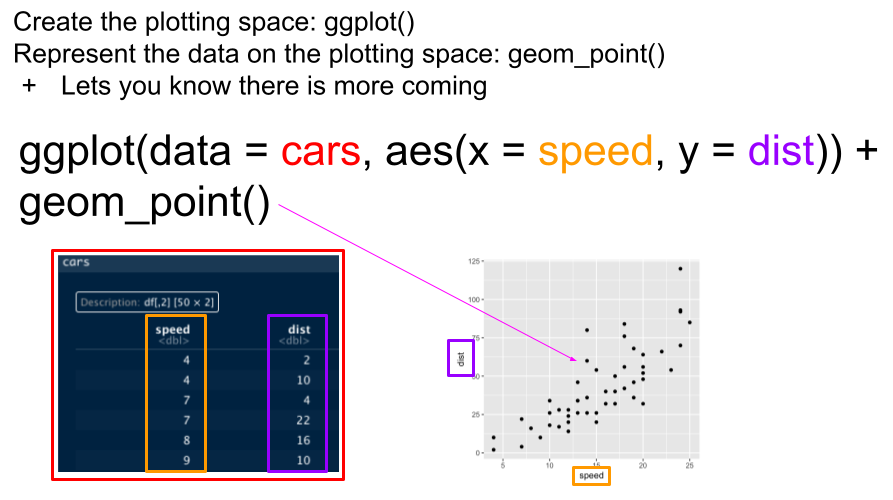
\includegraphics{images/GGplot syntax.png}
\caption{Basic ggplot syntax}
\end{figure}

\hypertarget{our-first-ggplot}{%
\section{Our first ggplot}\label{our-first-ggplot}}

Let's look at the Pine data, plotting streamflow (the cfs column) by the date (datetime column). We will show the time series as a line.

\begin{Shaded}
\begin{Highlighting}[]
\FunctionTok{ggplot}\NormalTok{(}\AttributeTok{data =}\NormalTok{ Pine, }\FunctionTok{aes}\NormalTok{(}\AttributeTok{x =}\NormalTok{ datetime, }\AttributeTok{y =}\NormalTok{ cfs))}\SpecialCharTok{+}
  \FunctionTok{geom\_line}\NormalTok{()}
\end{Highlighting}
\end{Shaded}

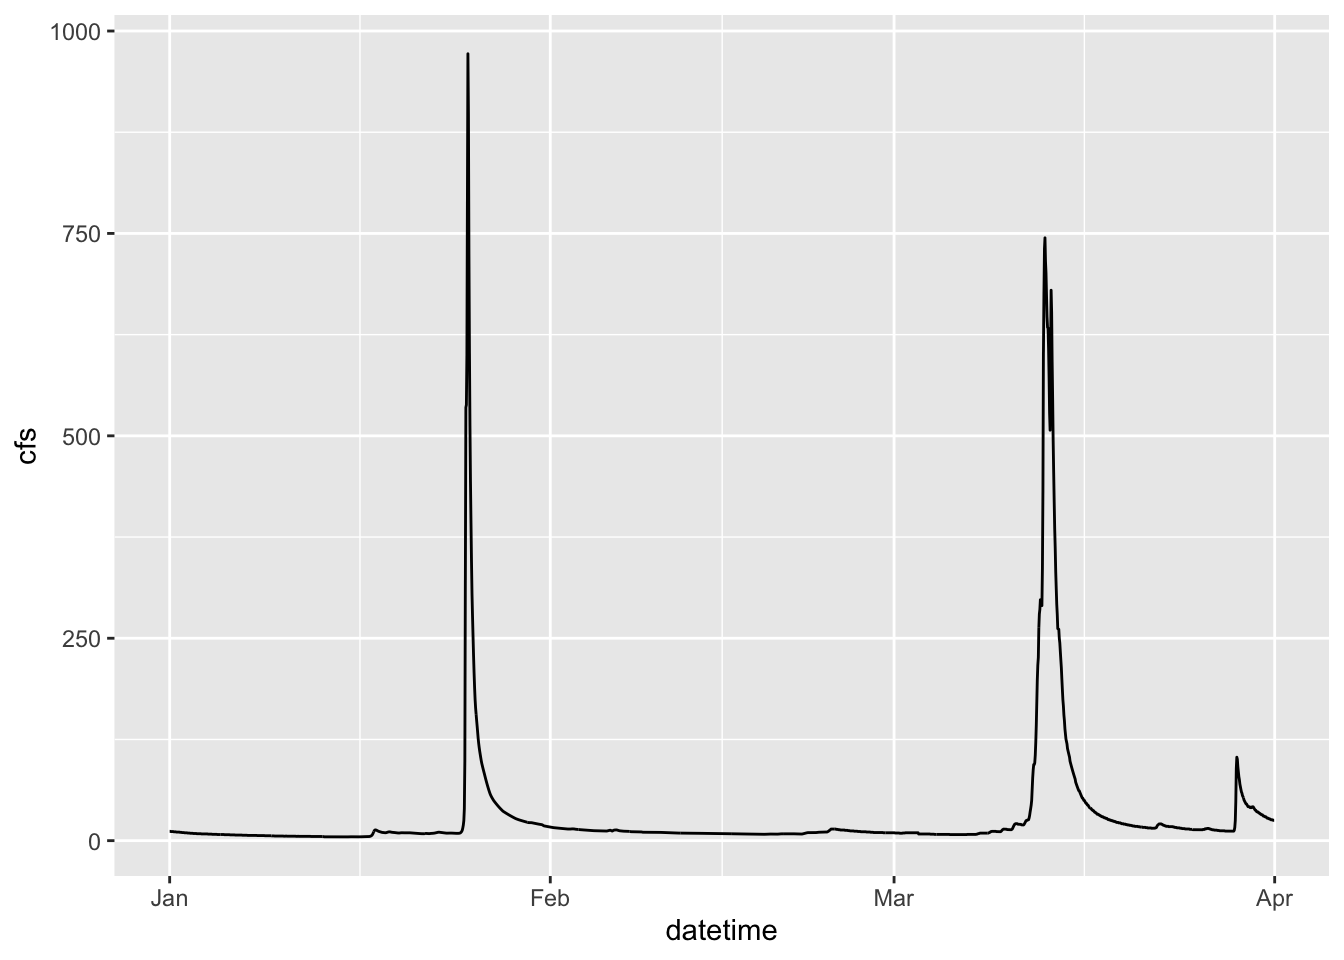
\includegraphics{Hydroinformatics_Bookdown_files/figure-latex/unnamed-chunk-5-1.pdf}

\hypertarget{change-point-type}{%
\section{Change point type}\label{change-point-type}}

Now let's make the same plot but show the data as points, using the pch parameter in geom\_point() we can change the point type to any of the following:

\begin{figure}
\centering
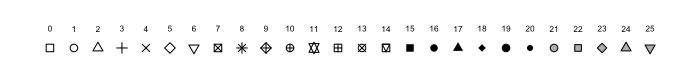
\includegraphics{images/pch.png}
\caption{pch options from R help file}
\end{figure}

\begin{Shaded}
\begin{Highlighting}[]
\FunctionTok{ggplot}\NormalTok{(}\AttributeTok{data =}\NormalTok{ Pine, }\FunctionTok{aes}\NormalTok{(}\AttributeTok{x =}\NormalTok{ datetime, }\AttributeTok{y =}\NormalTok{ cfs))}\SpecialCharTok{+}
  \FunctionTok{geom\_point}\NormalTok{(}\AttributeTok{pch =} \DecValTok{8}\NormalTok{)}
\end{Highlighting}
\end{Shaded}

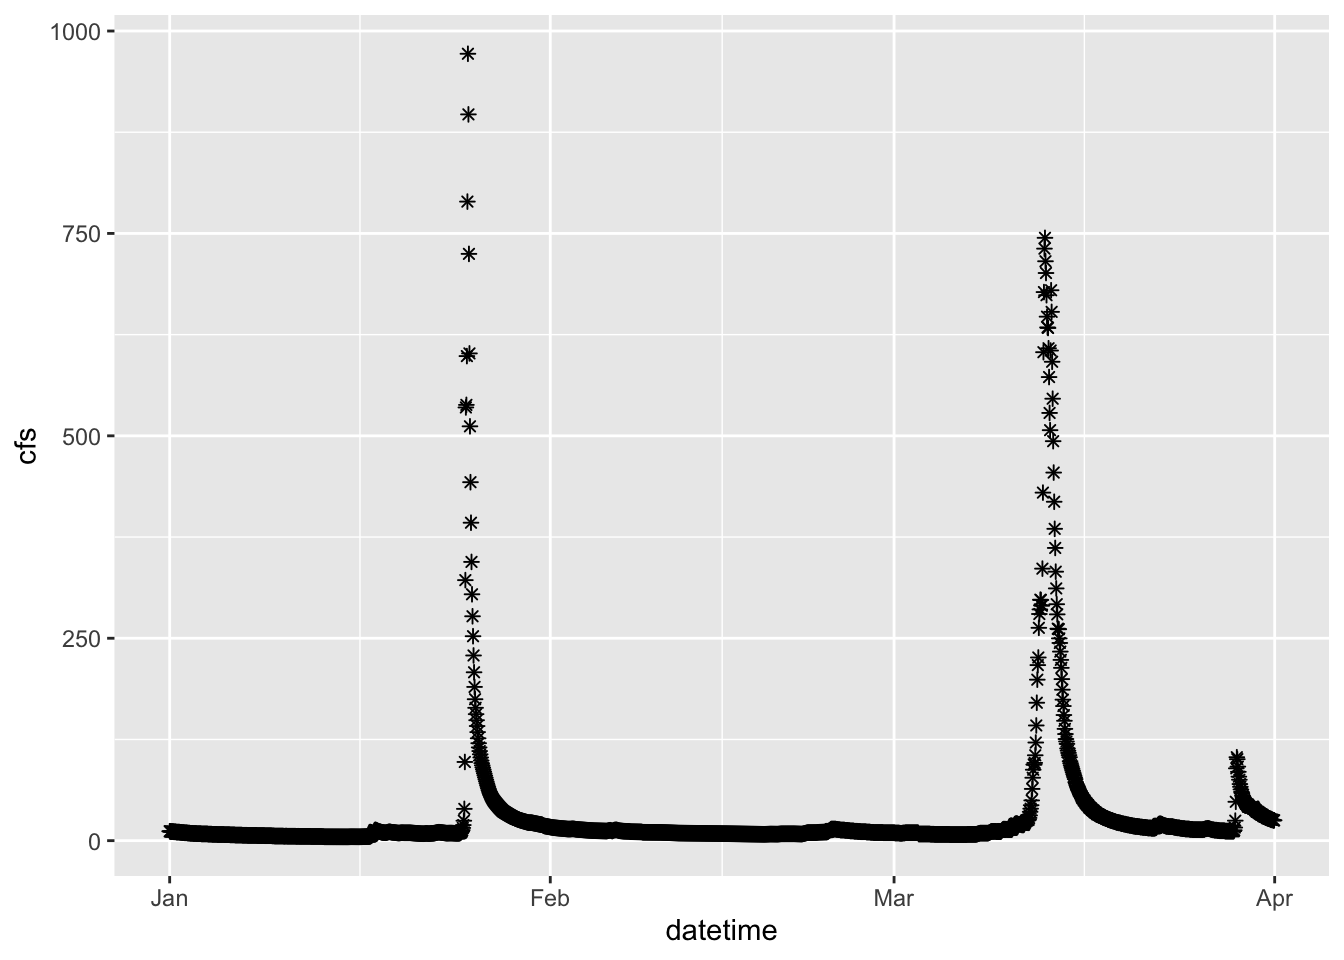
\includegraphics{Hydroinformatics_Bookdown_files/figure-latex/unnamed-chunk-6-1.pdf}

\hypertarget{set-colors}{%
\section{Set colors}\label{set-colors}}

We can also ``easily'' change the color. Easily is in quotes because this often trips people up. If you put color = ``blue'' in the aesthetic function, think about what that is telling ggplot. It says ``control the color using''blue"". That doesn't make a whole lot of sense, so neither does the output\ldots{} Try it.

What happens is that if color = ``blue'' is in the aesthetic, you are telling R that the color used in the geom represents ``blue''. This is very useful if you have multiple geoms in your plot, are coloring them differently, and are building a legend. But if you are just trying to color the points, it kind of feels like R is trolling you\ldots{} doesn't it?

Take the color = ``blue'' out of the aesthetic and you're golden.

\begin{Shaded}
\begin{Highlighting}[]
\FunctionTok{ggplot}\NormalTok{(}\AttributeTok{data =}\NormalTok{ Pine, }\FunctionTok{aes}\NormalTok{(datetime, }\AttributeTok{y =}\NormalTok{ cfs, }\AttributeTok{color =} \StringTok{"blue"}\NormalTok{))}\SpecialCharTok{+}
  \FunctionTok{geom\_point}\NormalTok{()}
\end{Highlighting}
\end{Shaded}

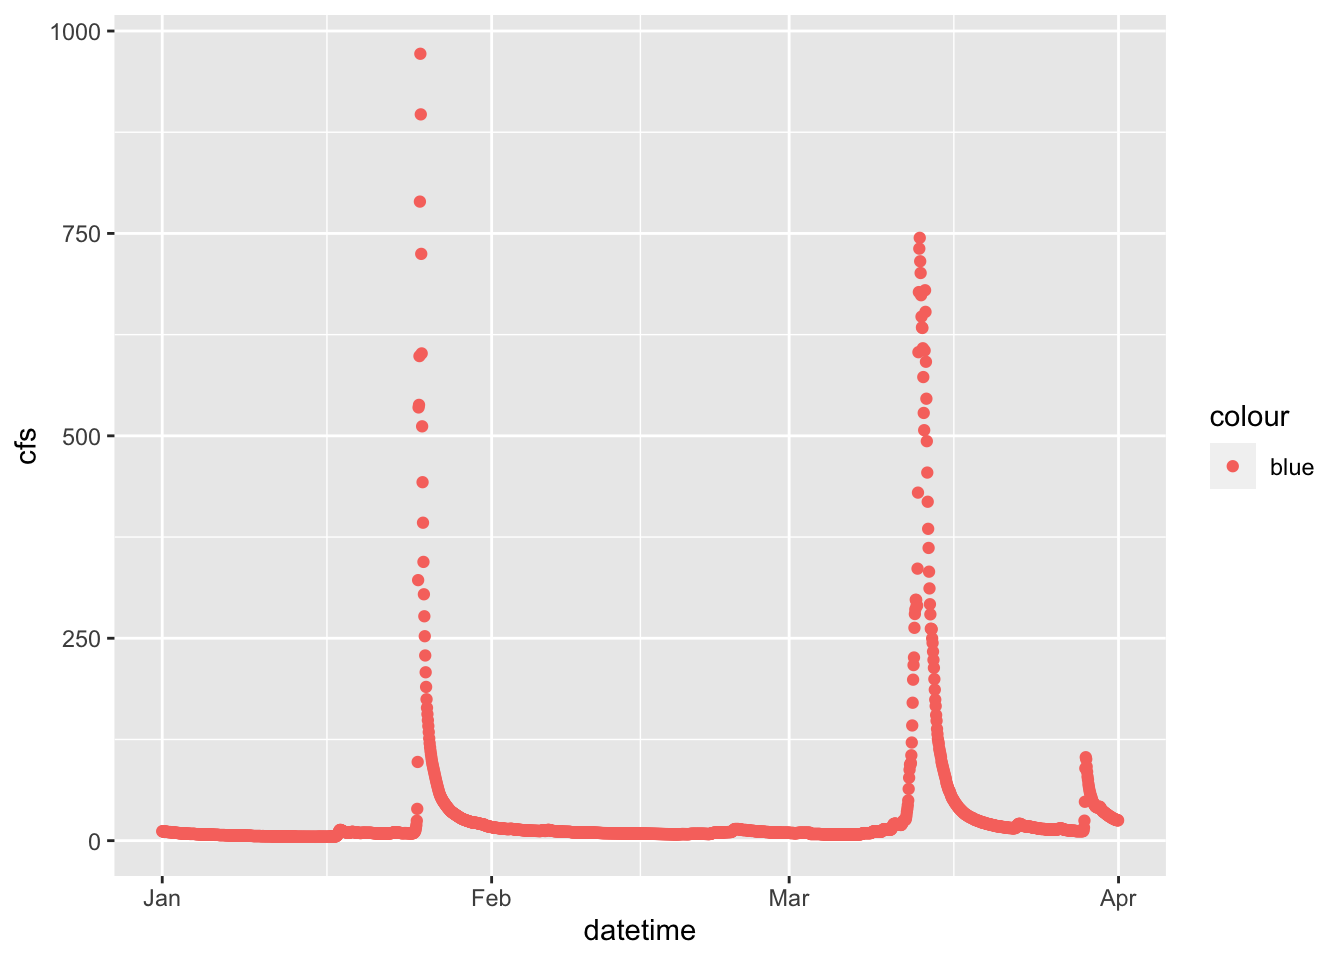
\includegraphics{Hydroinformatics_Bookdown_files/figure-latex/unnamed-chunk-7-1.pdf}

\begin{Shaded}
\begin{Highlighting}[]
\FunctionTok{ggplot}\NormalTok{(}\AttributeTok{data =}\NormalTok{ Pine, }\FunctionTok{aes}\NormalTok{(}\AttributeTok{x =}\NormalTok{ datetime, }\AttributeTok{y =}\NormalTok{ cfs))}\SpecialCharTok{+}
  \FunctionTok{geom\_point}\NormalTok{(}\AttributeTok{color =} \StringTok{"blue"}\NormalTok{)}
\end{Highlighting}
\end{Shaded}

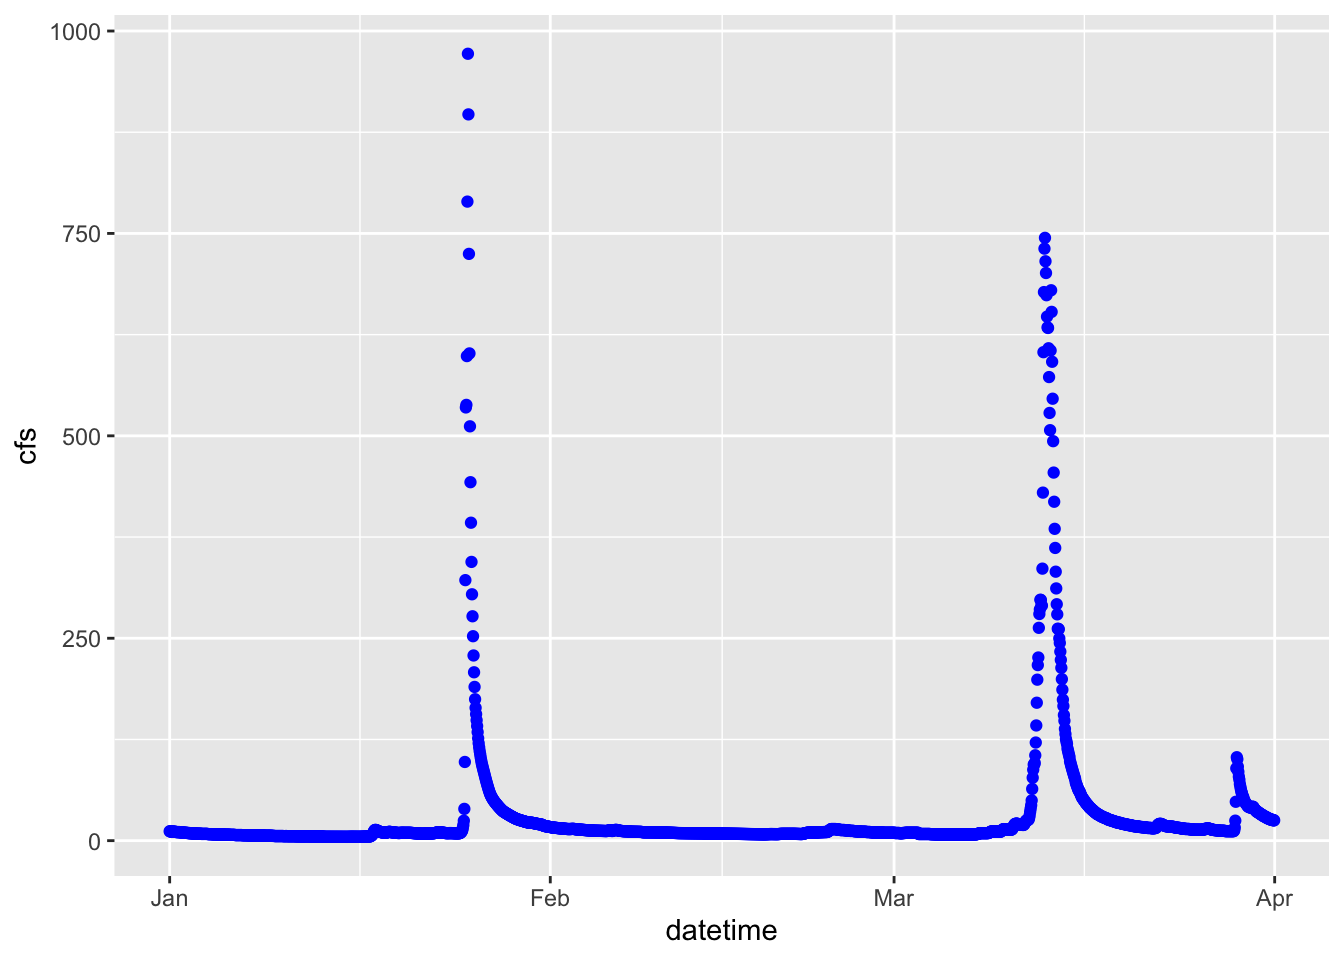
\includegraphics{Hydroinformatics_Bookdown_files/figure-latex/unnamed-chunk-7-2.pdf}

\hypertarget{controlling-color-with-a-third-variable-and-other-functions}{%
\section{Controlling color with a third variable and other functions}\label{controlling-color-with-a-third-variable-and-other-functions}}

Let's plot the data as a line again, but play with it a bit.

First: make the line blue

Second: change the theme

Third: change the axis labels

Fourth: color by discharge

\begin{Shaded}
\begin{Highlighting}[]
\FunctionTok{ggplot}\NormalTok{(}\AttributeTok{data =}\NormalTok{ Pine, }\FunctionTok{aes}\NormalTok{(}\AttributeTok{x =}\NormalTok{ datetime, }\AttributeTok{y =}\NormalTok{ cfs, }\AttributeTok{color =}\NormalTok{ cfs))}\SpecialCharTok{+}
  \FunctionTok{geom\_line}\NormalTok{()}\SpecialCharTok{+}
  \FunctionTok{ylab}\NormalTok{(}\StringTok{"Discharge (cfs)"}\NormalTok{)}\SpecialCharTok{+}
  \FunctionTok{xlab}\NormalTok{(}\FunctionTok{element\_blank}\NormalTok{())}\SpecialCharTok{+}
  \FunctionTok{theme\_classic}\NormalTok{()}
\end{Highlighting}
\end{Shaded}

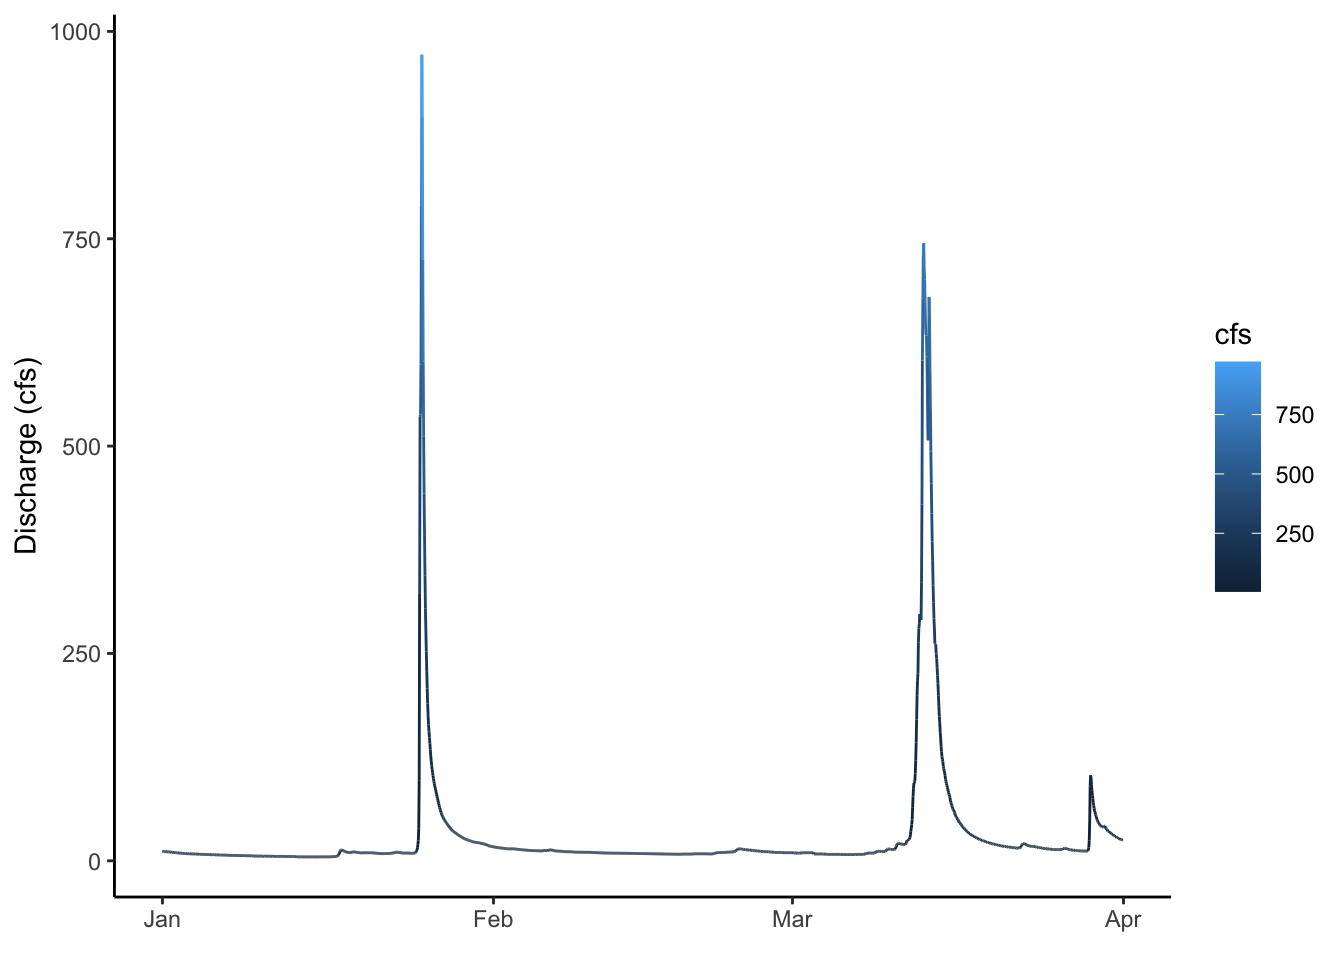
\includegraphics{Hydroinformatics_Bookdown_files/figure-latex/unnamed-chunk-8-1.pdf}

\hypertarget{plotting-multiple-groups}{%
\section{Plotting multiple groups}\label{plotting-multiple-groups}}

The SNP dataset has two different streams: Pine and NFDR

We can look at the two of those a couple of different ways

First, make two lines, colored by the stream by adding color = to your aesthetic.

\begin{Shaded}
\begin{Highlighting}[]
\FunctionTok{ggplot}\NormalTok{(}\AttributeTok{data =}\NormalTok{ SNP, }\FunctionTok{aes}\NormalTok{(}\AttributeTok{x =}\NormalTok{ datetime,}\AttributeTok{y =}\NormalTok{ cfs, }\AttributeTok{color =}\NormalTok{ StationID)) }\SpecialCharTok{+}
  \FunctionTok{geom\_line}\NormalTok{()}
\end{Highlighting}
\end{Shaded}

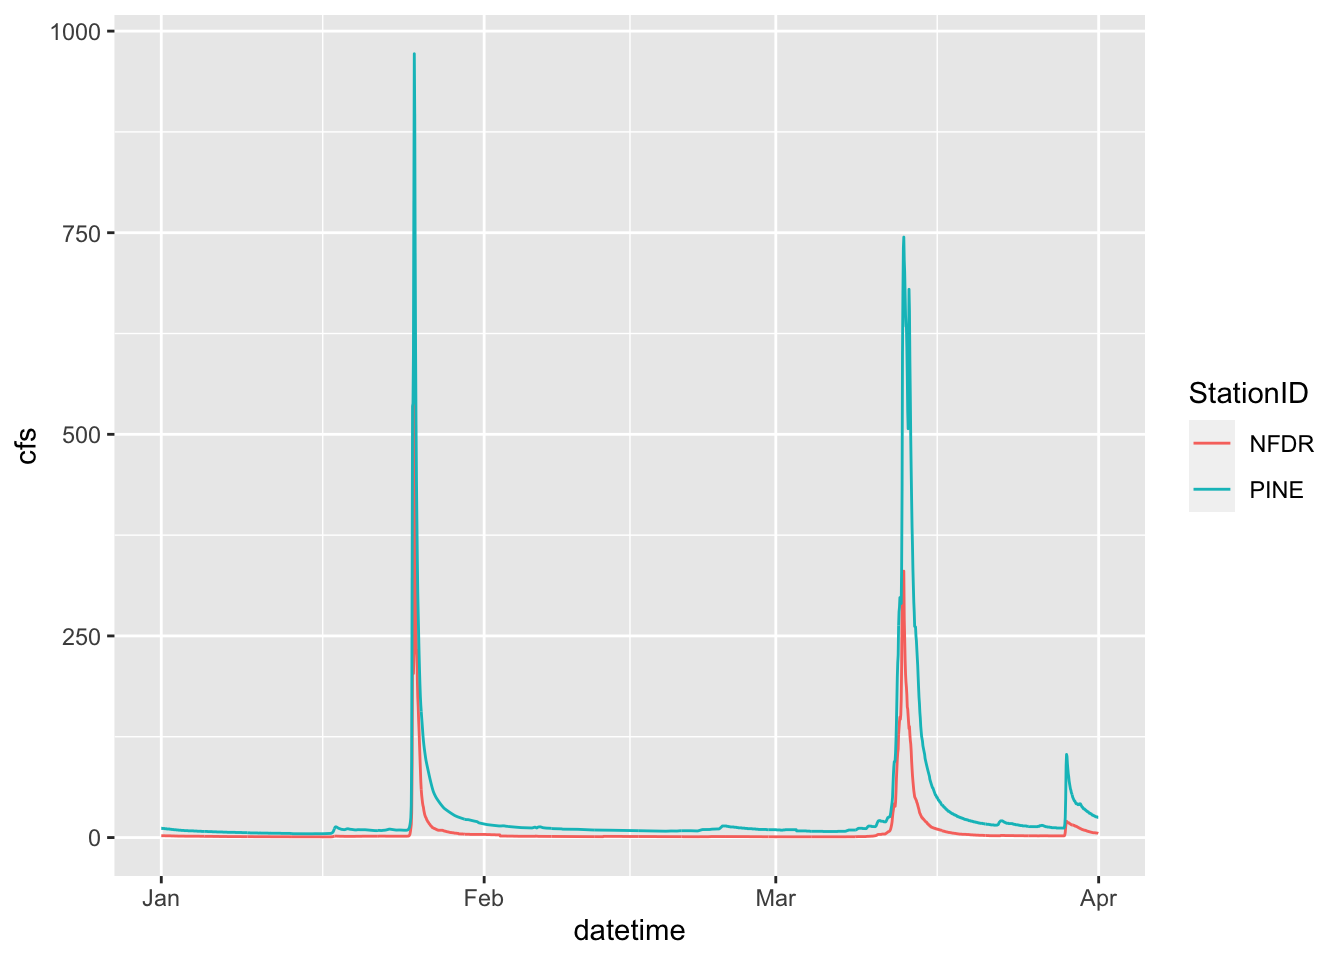
\includegraphics{Hydroinformatics_Bookdown_files/figure-latex/unnamed-chunk-9-1.pdf}

\hypertarget{facets}{%
\section{Facets}\label{facets}}

We can also use facets.

You must tell the facet\_wrap what variable to use to make the separate panels (facet =). It'll decide how to orient them or you can tell it how. We want them to be on top of each other so we are going to tell it we want 2 rows by setting nrow = 2. Note that we have to put the column used to make the facets in quotes after facets =

\begin{Shaded}
\begin{Highlighting}[]
\FunctionTok{ggplot}\NormalTok{(}\AttributeTok{data =}\NormalTok{ SNP, }\FunctionTok{aes}\NormalTok{(}\AttributeTok{x =}\NormalTok{ datetime,}\AttributeTok{y =}\NormalTok{ cfs)) }\SpecialCharTok{+}
  \FunctionTok{geom\_line}\NormalTok{() }\SpecialCharTok{+}
  \FunctionTok{facet\_wrap}\NormalTok{(}\AttributeTok{facets =} \StringTok{"StationID"}\NormalTok{, }\AttributeTok{nrow =} \DecValTok{2}\NormalTok{)}
\end{Highlighting}
\end{Shaded}

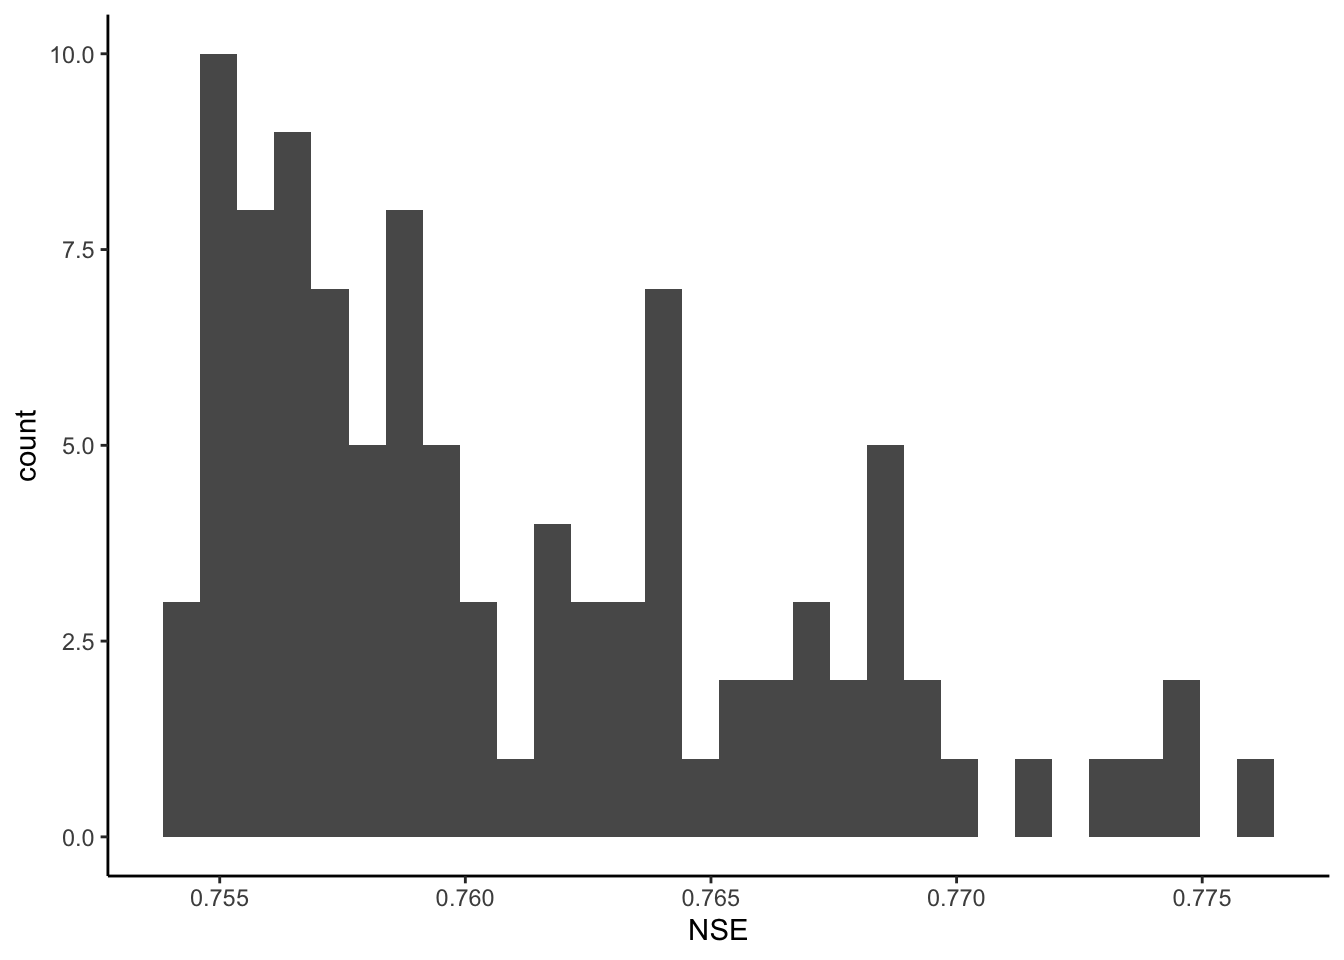
\includegraphics{Hydroinformatics_Bookdown_files/figure-latex/unnamed-chunk-10-1.pdf}

\hypertarget{two-variable-faceting}{%
\section{Two variable faceting}\label{two-variable-faceting}}

You can also use facet\_grid() to break your plots up into panels based on two variables. Below we will create a panel for each month in each watershed. Adding scales = ``free'' allows facet\_grid to change the axes. By default, all axes will be the same. This is often what we want, so we can more easily compare magnitudes, but sometimes we are looking for patterns more, so we may want to let the axes have whatever range works for the individual plots.

\begin{Shaded}
\begin{Highlighting}[]
\FunctionTok{ggplot}\NormalTok{(}\AttributeTok{data =}\NormalTok{ SNP, }\FunctionTok{aes}\NormalTok{(}\AttributeTok{x =}\NormalTok{ datetime,}\AttributeTok{y =}\NormalTok{ cfs)) }\SpecialCharTok{+}
  \FunctionTok{geom\_line}\NormalTok{() }\SpecialCharTok{+}
  \FunctionTok{facet\_grid}\NormalTok{(StationID }\SpecialCharTok{\textasciitilde{}}\NormalTok{ month, }\AttributeTok{scales =} \StringTok{"free"}\NormalTok{)}
\end{Highlighting}
\end{Shaded}

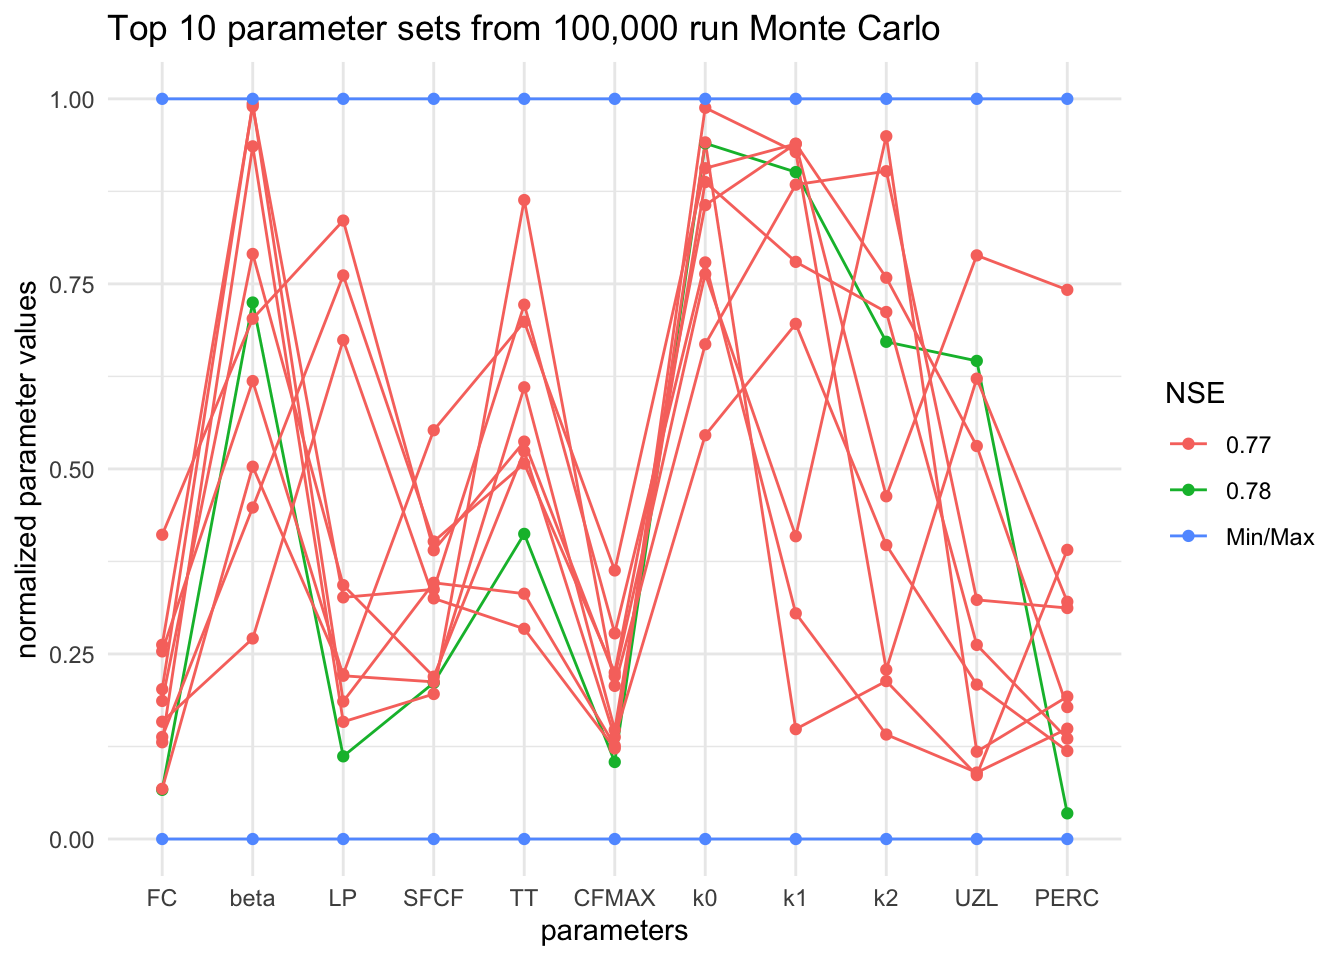
\includegraphics{Hydroinformatics_Bookdown_files/figure-latex/unnamed-chunk-11-1.pdf}

\hypertarget{boxplots}{%
\section{Boxplots}\label{boxplots}}

We can look at these data in other ways as well. A very useful way to look at the variation of two groups is to use a boxplot.

Because the data span several orders of magnitude, we will have to log the y axis to see the differences between the two streams. We do that by adding scale\_y\_log10()

\begin{Shaded}
\begin{Highlighting}[]
\FunctionTok{ggplot}\NormalTok{(}\AttributeTok{data =}\NormalTok{ SNP, }\FunctionTok{aes}\NormalTok{(}\AttributeTok{x =}\NormalTok{ StationID, }\AttributeTok{y =}\NormalTok{ cfs)) }\SpecialCharTok{+} 
  \FunctionTok{stat\_boxplot}\NormalTok{()}\SpecialCharTok{+}
  \FunctionTok{scale\_y\_log10}\NormalTok{()}
\end{Highlighting}
\end{Shaded}

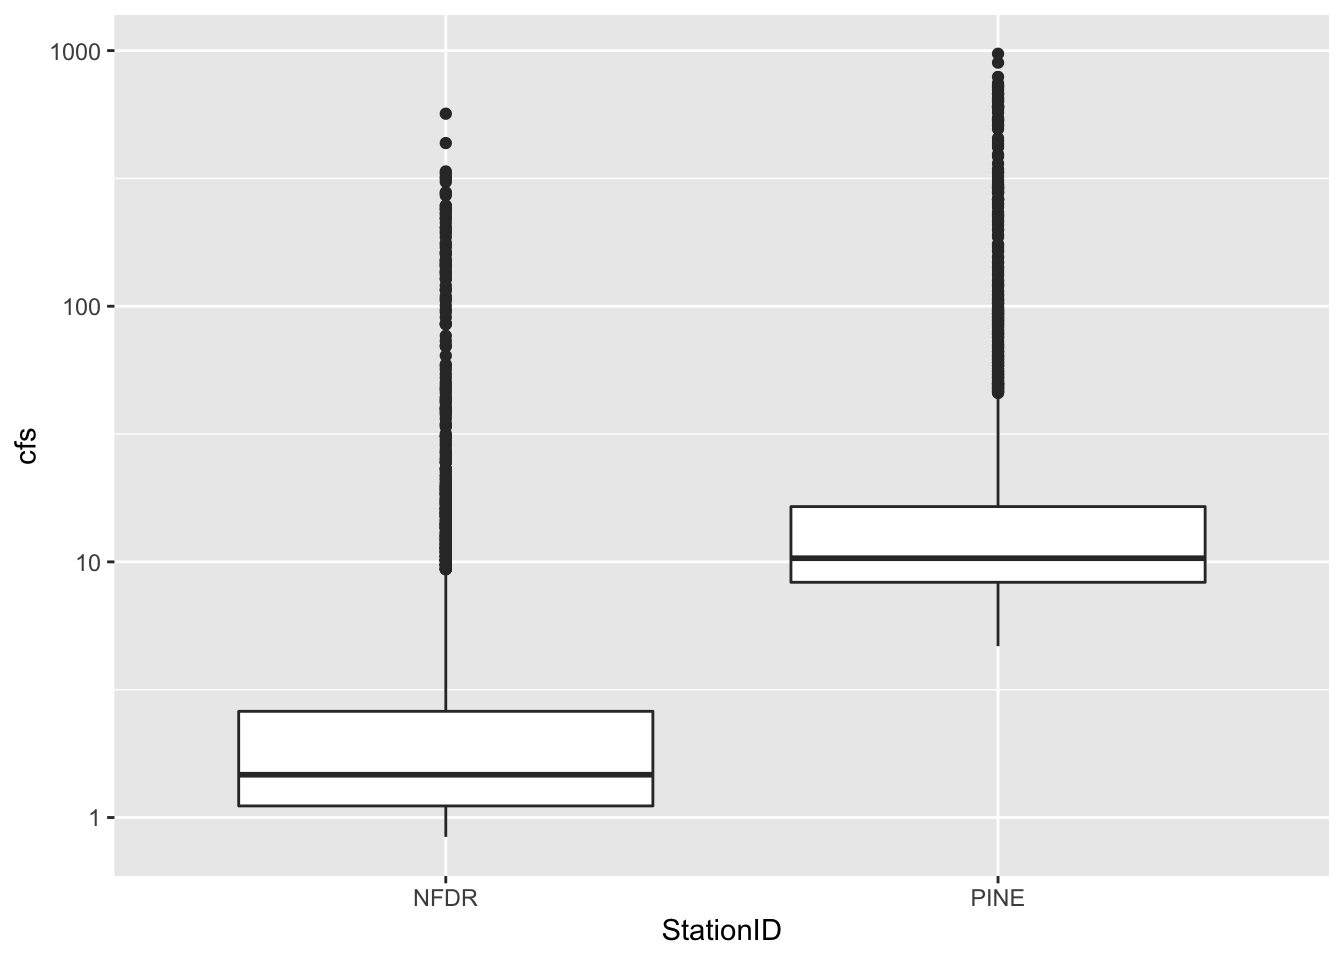
\includegraphics{Hydroinformatics_Bookdown_files/figure-latex/unnamed-chunk-12-1.pdf}

\hypertarget{more-about-color-size-etc}{%
\section{More about color, size, etc}\label{more-about-color-size-etc}}

Let's play around a bit with controlling color, point size, etc with other data.

We can control the size of points by putting size = in the aes() and color by putting color =

If you use a point type that has a background, like \#21, you can also set the background color using bg =

If points are too close together to see them all you can use a hollow point type or set the alpha lower so the points are transparent (alpha = )

\begin{Shaded}
\begin{Highlighting}[]
\FunctionTok{ggplot}\NormalTok{(RBI, }\FunctionTok{aes}\NormalTok{(RBI, DRAIN\_SQKM, }\AttributeTok{size =}\NormalTok{ T\_AVG\_SITE, }\AttributeTok{bg =}\NormalTok{ STATE))}\SpecialCharTok{+}
  \FunctionTok{geom\_point}\NormalTok{(}\AttributeTok{pch =} \DecValTok{21}\NormalTok{, }\AttributeTok{alpha =} \FloatTok{0.3}\NormalTok{)}
\end{Highlighting}
\end{Shaded}

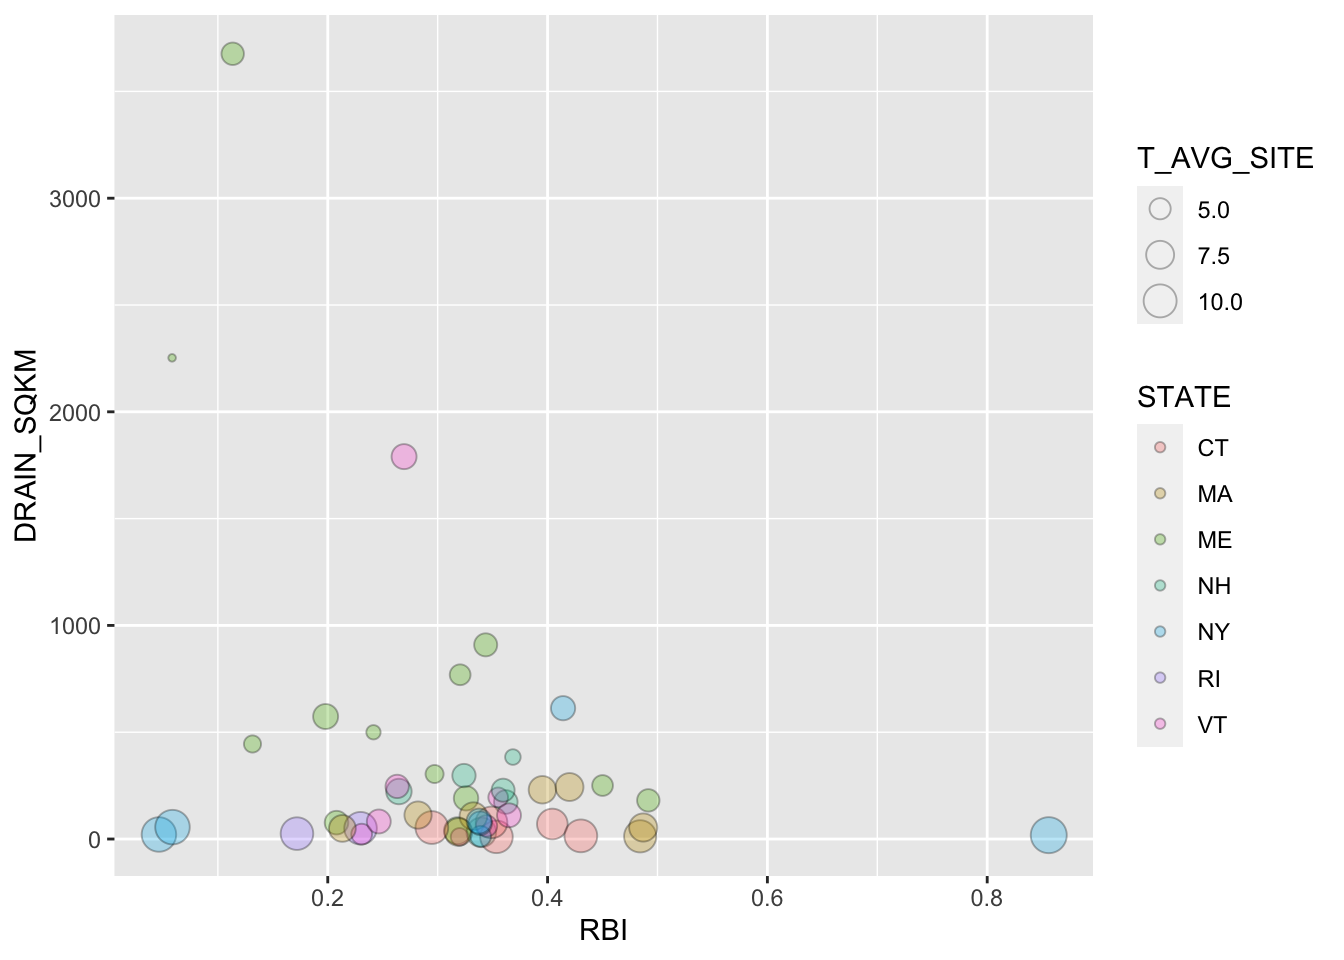
\includegraphics{Hydroinformatics_Bookdown_files/figure-latex/unnamed-chunk-13-1.pdf}

\hypertarget{multiple-geoms}{%
\section{Multiple geoms}\label{multiple-geoms}}

Finally: You can add multiple geoms to the same plot. Examples of when you might want to do this are when you are showing a line fit and want to show the points as well, or maybe showing a boxplot and want to show the data behind it. You simply add additional geom\_\ldots{} lines to add additional geoms.

\begin{Shaded}
\begin{Highlighting}[]
\FunctionTok{ggplot}\NormalTok{(RBI, }\FunctionTok{aes}\NormalTok{(RBI, DRAIN\_SQKM, }\AttributeTok{color =}\NormalTok{ AGGECOREGION))}\SpecialCharTok{+}
  \FunctionTok{stat\_smooth}\NormalTok{(}\AttributeTok{method =} \StringTok{"lm"}\NormalTok{, }\AttributeTok{linetype =} \DecValTok{2}\NormalTok{)}\SpecialCharTok{+}
  \FunctionTok{geom\_point}\NormalTok{()}
\end{Highlighting}
\end{Shaded}

\begin{verbatim}
## `geom_smooth()` using formula 'y ~ x'
\end{verbatim}

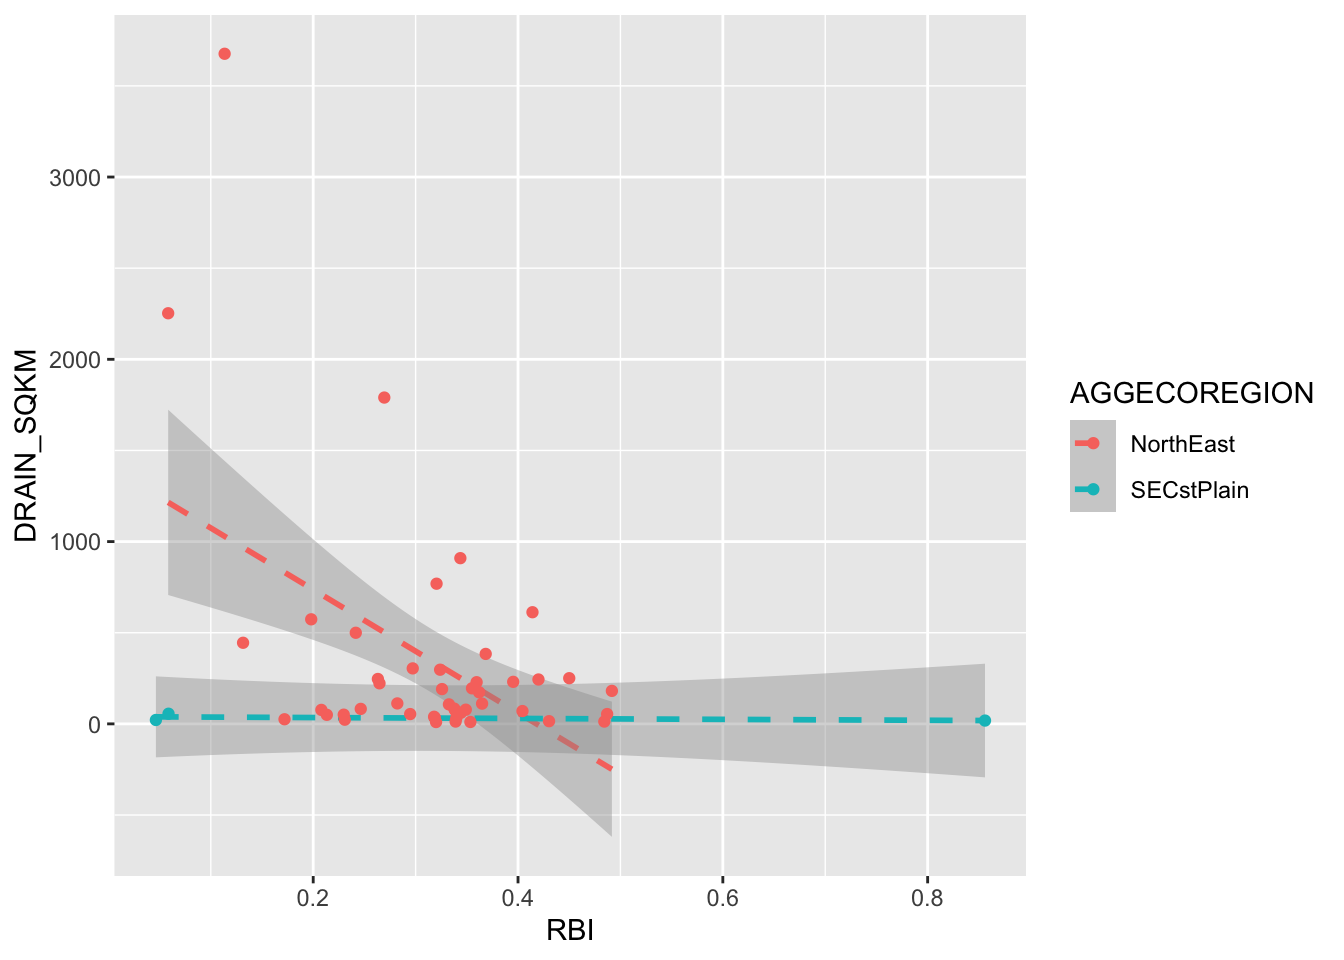
\includegraphics{Hydroinformatics_Bookdown_files/figure-latex/unnamed-chunk-14-1.pdf}

\hypertarget{Programming}{%
\chapter{R Tidyverse Programming Basics}\label{Programming}}

Get this document and a version with empty code chunks at the template repository on github: \url{https://github.com/VT-Hydroinformatics/2-Programming-Basics}

\hypertarget{introduction-1}{%
\section{Introduction}\label{introduction-1}}

We have messed around with plotting a bit and you've seen a little of what R can do. So now let's review or introduce you to some basics. Even if you have worked in R before, it is good to be remind of/practice with this stuff, so stay tuned in!

This exercise covers most of the same principles as two chapters in R for Data Science

Workflow: basics (\url{https://r4ds.had.co.nz/workflow-basics.html})

Data transformation (\url{https://r4ds.had.co.nz/transform.html})

\hypertarget{you-can-use-r-as-a-calculator}{%
\section{You can use R as a calculator}\label{you-can-use-r-as-a-calculator}}

If you just type numbers and operators in, R will spit out the results

\begin{Shaded}
\begin{Highlighting}[]
\DecValTok{1} \SpecialCharTok{+} \DecValTok{2}
\end{Highlighting}
\end{Shaded}

\begin{verbatim}
## [1] 3
\end{verbatim}

\hypertarget{you-can-create-new-objects-using--}{%
\section{You can create new objects using \textless-}\label{you-can-create-new-objects-using--}}

Yea yea, = does the same thing. But use \textless-. We will call \textless- assignment or assignment operator. When we are coding in R we use \textless- to assign values to objects and = to set values for parameters in functions. Using \textless- helps us differentiate between the two. Norms for formatting are important because they help us understand what code is doing, especially when stuff gets complex.

Oh, one more thing: Surround operators with spaces. Don't code like a gorilla.

x \textless- 1 looks better than x\textless-1 and if you disagree you are wrong. :)

You can assign single numbers or entire chunks of data using \textless-

So if you had an object called my\_data and wanted to copy it into my\_new\_data you could do:

my\_new\_data \textless- my\_data

You can then recall/print the values in an object by just typing the name by itself.

In the code chunk below, assign a 3 to the object ``y'' and then print it out.

\begin{Shaded}
\begin{Highlighting}[]
\NormalTok{y }\OtherTok{\textless{}{-}} \DecValTok{3}
\NormalTok{y}
\end{Highlighting}
\end{Shaded}

\begin{verbatim}
## [1] 3
\end{verbatim}

If you want to assign multiple values, you have to put them in the function c() c means combine. R doesn't know what to do if you just give it a bunch of values with space or commas, but if you put them as arguments in the combine function, it'll make them into a vector.

Any time you need to use several values, even passing as an argument to a function, you have to put them in c() or it won't work.

\begin{Shaded}
\begin{Highlighting}[]
\NormalTok{a }\OtherTok{\textless{}{-}} \FunctionTok{c}\NormalTok{(}\DecValTok{1}\NormalTok{,}\DecValTok{2}\NormalTok{,}\DecValTok{3}\NormalTok{,}\DecValTok{4}\NormalTok{)}
\NormalTok{a}
\end{Highlighting}
\end{Shaded}

\begin{verbatim}
## [1] 1 2 3 4
\end{verbatim}

When you are creating objects, try to give them meaningful names so you can remember what they are. You can't have spaces or operators that mean something else as part of a name. And remember, everything is case sensitive.

Assign the value 5.4 to water\_pH and then try to recall it by typing ``water\_ph''

\begin{Shaded}
\begin{Highlighting}[]
\NormalTok{water\_pH }\OtherTok{\textless{}{-}} \FloatTok{5.4}

\CommentTok{\#water\_ph}
\end{Highlighting}
\end{Shaded}

You can also set objects equal to strings, or values that have letters in them. To do this you just have to put the value in quotes, otherwise R will think it is an object name and tell you it doesn't exist.

Try: name \textless- ``JP'' and then name \textless- JP

What happens if you forget the ending parenthesis?

Try: name \textless- "JP

R can be cryptic with it's error messages or other responses, but once you get used to them, you know exactly what is wrong when they pop up.

\begin{Shaded}
\begin{Highlighting}[]
\NormalTok{name }\OtherTok{\textless{}{-}} \StringTok{"JP"}
\CommentTok{\#name \textless{}{-} JP}
\end{Highlighting}
\end{Shaded}

\hypertarget{using-functions}{%
\section{Using functions}\label{using-functions}}

\includegraphics{images/Function syntax.png}

As an example, let's try the seq() function, which creates a sequence of numbers.

\begin{Shaded}
\begin{Highlighting}[]
\FunctionTok{seq}\NormalTok{(}\AttributeTok{from =} \DecValTok{1}\NormalTok{, }\AttributeTok{to =} \DecValTok{10}\NormalTok{, }\AttributeTok{by =} \DecValTok{1}\NormalTok{)}
\end{Highlighting}
\end{Shaded}

\begin{verbatim}
##  [1]  1  2  3  4  5  6  7  8  9 10
\end{verbatim}

\begin{Shaded}
\begin{Highlighting}[]
\CommentTok{\#or}

\FunctionTok{seq}\NormalTok{(}\DecValTok{1}\NormalTok{, }\DecValTok{10}\NormalTok{, }\DecValTok{1}\NormalTok{)}
\end{Highlighting}
\end{Shaded}

\begin{verbatim}
##  [1]  1  2  3  4  5  6  7  8  9 10
\end{verbatim}

\begin{Shaded}
\begin{Highlighting}[]
\CommentTok{\#or}

\FunctionTok{seq}\NormalTok{(}\DecValTok{1}\NormalTok{, }\DecValTok{10}\NormalTok{)}
\end{Highlighting}
\end{Shaded}

\begin{verbatim}
##  [1]  1  2  3  4  5  6  7  8  9 10
\end{verbatim}

\begin{Shaded}
\begin{Highlighting}[]
\CommentTok{\#what does this do}
\FunctionTok{seq}\NormalTok{(}\DecValTok{10}\NormalTok{,}\DecValTok{1}\NormalTok{)}
\end{Highlighting}
\end{Shaded}

\begin{verbatim}
##  [1] 10  9  8  7  6  5  4  3  2  1
\end{verbatim}

\hypertarget{read-in-some-data.}{%
\section{Read in some data.}\label{read-in-some-data.}}

For the following demonstration we will use the RBI data from a sample of USGS gages we used last class. First we will load the tidyverse library, everything we have done so far is in base R.

Important: read\_csv() is the tidyverse csv reading function, the base R function is read.csv(). read.csv() will not read your data in as a tibble, which is the format used by tidyverse functions.

\begin{Shaded}
\begin{Highlighting}[]
\FunctionTok{library}\NormalTok{(tidyverse)}

\NormalTok{rbi }\OtherTok{\textless{}{-}} \FunctionTok{read\_csv}\NormalTok{(}\StringTok{"Flashy\_Dat\_Subset.csv"}\NormalTok{)}
\end{Highlighting}
\end{Shaded}

\begin{verbatim}
## 
## -- Column specification --------------------------------------------------------
## cols(
##   .default = col_double(),
##   STANAME = col_character(),
##   STATE = col_character(),
##   CLASS = col_character(),
##   AGGECOREGION = col_character()
## )
## i Use `spec()` for the full column specifications.
\end{verbatim}

\hypertarget{wait-hold-up.-what-is-a-tibble}{%
\section{Wait, hold up. What is a tibble?}\label{wait-hold-up.-what-is-a-tibble}}

Good question. It's a fancy way to store data that works well with tidyverse functions. Let's look at the rbi tibble.

\begin{Shaded}
\begin{Highlighting}[]
\FunctionTok{head}\NormalTok{(rbi)}
\end{Highlighting}
\end{Shaded}

\begin{verbatim}
## # A tibble: 6 x 26
##   site_no    RBI RBIrank STANAME  DRAIN_SQKM HUC02 LAT_GAGE LNG_GAGE STATE CLASS
##     <dbl>  <dbl>   <dbl> <chr>         <dbl> <dbl>    <dbl>    <dbl> <chr> <chr>
## 1 1013500 0.0584      35 Fish Ri~     2253.      1     47.2    -68.6 ME    Ref  
## 2 1021480 0.208      300 Old Str~       76.7     1     44.9    -67.7 ME    Ref  
## 3 1022500 0.198      286 Narragu~      574.      1     44.6    -67.9 ME    Ref  
## 4 1029200 0.132      183 Seboeis~      445.      1     46.1    -68.6 ME    Ref  
## 5 1030500 0.114      147 Mattawa~     3676.      1     45.5    -68.3 ME    Ref  
## 6 1031300 0.297      489 Piscata~      304.      1     45.3    -69.6 ME    Ref  
## # ... with 16 more variables: AGGECOREGION <chr>, PPTAVG_BASIN <dbl>,
## #   PPTAVG_SITE <dbl>, T_AVG_BASIN <dbl>, T_AVG_SITE <dbl>, T_MAX_BASIN <dbl>,
## #   T_MAXSTD_BASIN <dbl>, T_MAX_SITE <dbl>, T_MIN_BASIN <dbl>,
## #   T_MINSTD_BASIN <dbl>, T_MIN_SITE <dbl>, PET <dbl>, SNOW_PCT_PRECIP <dbl>,
## #   PRECIP_SEAS_IND <dbl>, FLOWYRS_1990_2009 <dbl>, wy00_09 <dbl>
\end{verbatim}

Now read in the same data with read.csv() which will NOT read the data as a tibble. How is it different? Output each one in the Console.

Knowing the data type for each column is super helpful for a few reasons\ldots. let's talk about them.

Types: int, dbl, fctr, char, logical

\begin{Shaded}
\begin{Highlighting}[]
\NormalTok{rbi\_NT }\OtherTok{\textless{}{-}} \FunctionTok{read.csv}\NormalTok{(}\StringTok{"Flashy\_Dat\_Subset.csv"}\NormalTok{)}

\FunctionTok{head}\NormalTok{(rbi\_NT)}
\end{Highlighting}
\end{Shaded}

\begin{verbatim}
##   site_no        RBI RBIrank                                     STANAME
## 1 1013500 0.05837454      35            Fish River near Fort Kent, Maine
## 2 1021480 0.20797008     300               Old Stream near Wesley, Maine
## 3 1022500 0.19805382     286     Narraguagus River at Cherryfield, Maine
## 4 1029200 0.13151299     183         Seboeis River near Shin Pond, Maine
## 5 1030500 0.11350485     147 Mattawamkeag River near Mattawamkeag, Maine
## 6 1031300 0.29718786     489       Piscataquis River at Blanchard, Maine
##   DRAIN_SQKM HUC02 LAT_GAGE  LNG_GAGE STATE CLASS AGGECOREGION PPTAVG_BASIN
## 1     2252.7     1 47.23739 -68.58264    ME   Ref    NorthEast        97.42
## 2       76.7     1 44.93694 -67.73611    ME   Ref    NorthEast       115.39
## 3      573.6     1 44.60797 -67.93524    ME   Ref    NorthEast       120.07
## 4      444.9     1 46.14306 -68.63361    ME   Ref    NorthEast       102.19
## 5     3676.2     1 45.50097 -68.30596    ME   Ref    NorthEast       108.19
## 6      304.4     1 45.26722 -69.58389    ME   Ref    NorthEast       119.83
##   PPTAVG_SITE T_AVG_BASIN T_AVG_SITE T_MAX_BASIN T_MAXSTD_BASIN T_MAX_SITE
## 1       93.53        3.00        3.0        9.67          0.202       10.0
## 2      117.13        5.71        5.8       11.70          0.131       11.9
## 3      129.56        5.95        6.3       11.90          0.344       12.2
## 4      103.24        3.61        4.0        9.88          0.231       10.4
## 5      113.13        4.82        5.4       10.75          0.554       11.7
## 6      120.93        3.60        4.2        9.57          0.431       11.0
##   T_MIN_BASIN T_MINSTD_BASIN T_MIN_SITE   PET SNOW_PCT_PRECIP PRECIP_SEAS_IND
## 1       -2.49          0.269       -2.7 504.7            36.9           0.102
## 2       -0.85          0.123       -0.6 554.2            39.5           0.046
## 3        0.06          0.873        1.4 553.1            38.2           0.047
## 4       -2.13          0.216       -1.5 513.0            36.4           0.070
## 5       -1.49          0.251       -1.2 540.8            37.2           0.033
## 6       -2.46          0.268       -1.7 495.8            40.2           0.030
##   FLOWYRS_1990_2009 wy00_09
## 1                20      10
## 2                11      10
## 3                20      10
## 4                11      10
## 5                20      10
## 6                13      10
\end{verbatim}

\hypertarget{data-wrangling-in-dplyr}{%
\section{Data wrangling in dplyr}\label{data-wrangling-in-dplyr}}

If you forget syntax or what the following functions do, here is an excellent cheat sheet: \url{https://rstudio.com/wp-content/uploads/2015/02/data-wrangling-cheatsheet.pdf}

We will demo five functions below:

\begin{itemize}
\tightlist
\item
  \textbf{filter()} - returns rows that meet specified conditions
\item
  \textbf{arrange()} - reorders rows
\item
  \textbf{select()} - pull out variables (columns)
\item
  \textbf{mutate()} - create new variables (columns) or reformat existing ones
\item
  \textbf{summarize()} - collapse groups of values into summary stats
\end{itemize}

With all of these, the first argument is the data and then the arguments after that specify what you want the function to do.

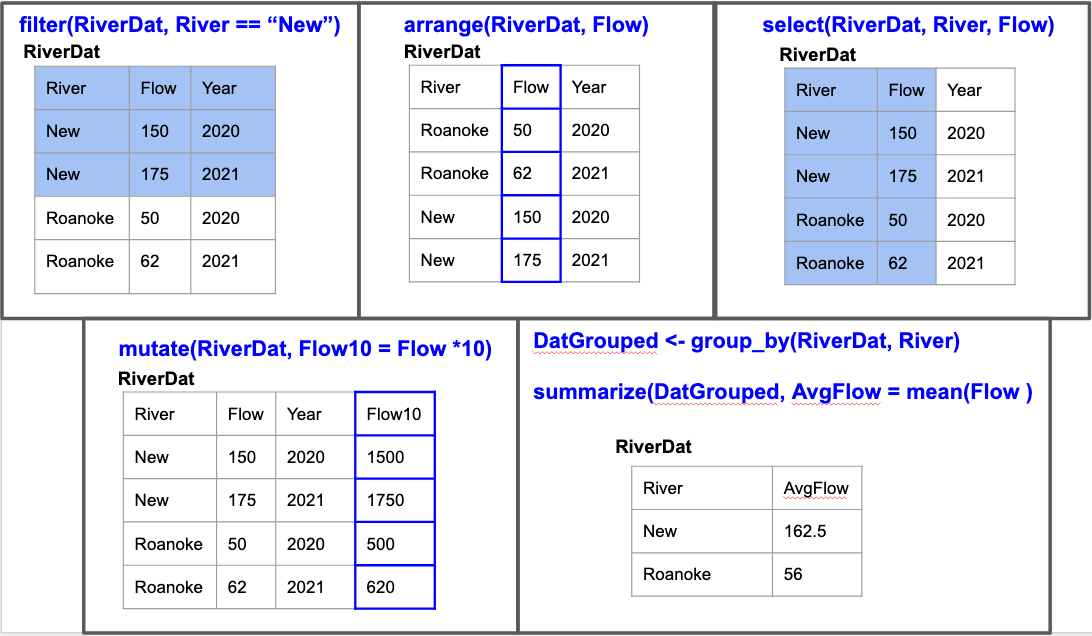
\includegraphics{images/dplyr functions.png}

\hypertarget{filter}{%
\section{Filter}\label{filter}}

Write an expression that returns data in rbi for the state of Maine (ME)

Operators:\\
== equal\\
!= not equal\\
\textgreater= , \textless= greater than or equal to, less than or equal to\\
\textgreater, \textless{} greater than or less then\\
\%in\% included in a list of values\\
\& and\\
\textbar{} or

\begin{Shaded}
\begin{Highlighting}[]
\FunctionTok{filter}\NormalTok{(rbi, STATE }\SpecialCharTok{==} \StringTok{"ME"}\NormalTok{)}
\end{Highlighting}
\end{Shaded}

\begin{verbatim}
## # A tibble: 13 x 26
##    site_no    RBI RBIrank STANAME DRAIN_SQKM HUC02 LAT_GAGE LNG_GAGE STATE CLASS
##      <dbl>  <dbl>   <dbl> <chr>        <dbl> <dbl>    <dbl>    <dbl> <chr> <chr>
##  1 1013500 0.0584      35 Fish R~     2253.      1     47.2    -68.6 ME    Ref  
##  2 1021480 0.208      300 Old St~       76.7     1     44.9    -67.7 ME    Ref  
##  3 1022500 0.198      286 Narrag~      574.      1     44.6    -67.9 ME    Ref  
##  4 1029200 0.132      183 Seboei~      445.      1     46.1    -68.6 ME    Ref  
##  5 1030500 0.114      147 Mattaw~     3676.      1     45.5    -68.3 ME    Ref  
##  6 1031300 0.297      489 Piscat~      304.      1     45.3    -69.6 ME    Ref  
##  7 1031500 0.320      545 Piscat~      769       1     45.2    -69.3 ME    Ref  
##  8 1037380 0.318      537 Ducktr~       39       1     44.3    -69.1 ME    Ref  
##  9 1044550 0.242      360 Spence~      500.      1     45.3    -70.2 ME    Ref  
## 10 1047000 0.344      608 Carrab~      909.      1     44.9    -70.0 ME    Ref  
## 11 1054200 0.492      805 Wild R~      181       1     44.4    -71.0 ME    Ref  
## 12 1055000 0.450      762 Swift ~      251.      1     44.6    -70.6 ME    Ref  
## 13 1057000 0.326      561 Little~      191.      1     44.3    -70.5 ME    Ref  
## # ... with 16 more variables: AGGECOREGION <chr>, PPTAVG_BASIN <dbl>,
## #   PPTAVG_SITE <dbl>, T_AVG_BASIN <dbl>, T_AVG_SITE <dbl>, T_MAX_BASIN <dbl>,
## #   T_MAXSTD_BASIN <dbl>, T_MAX_SITE <dbl>, T_MIN_BASIN <dbl>,
## #   T_MINSTD_BASIN <dbl>, T_MIN_SITE <dbl>, PET <dbl>, SNOW_PCT_PRECIP <dbl>,
## #   PRECIP_SEAS_IND <dbl>, FLOWYRS_1990_2009 <dbl>, wy00_09 <dbl>
\end{verbatim}

\hypertarget{multiple-conditions}{%
\subsection{Multiple conditions}\label{multiple-conditions}}

How many gages are there in Maine with an rbi greater than 0.25

\begin{Shaded}
\begin{Highlighting}[]
\FunctionTok{filter}\NormalTok{(rbi, STATE }\SpecialCharTok{==} \StringTok{"ME"} \SpecialCharTok{\&}\NormalTok{ RBI }\SpecialCharTok{\textgreater{}} \FloatTok{0.25}\NormalTok{)}
\end{Highlighting}
\end{Shaded}

\begin{verbatim}
## # A tibble: 7 x 26
##   site_no   RBI RBIrank STANAME   DRAIN_SQKM HUC02 LAT_GAGE LNG_GAGE STATE CLASS
##     <dbl> <dbl>   <dbl> <chr>          <dbl> <dbl>    <dbl>    <dbl> <chr> <chr>
## 1 1031300 0.297     489 Piscataq~       304.     1     45.3    -69.6 ME    Ref  
## 2 1031500 0.320     545 Piscataq~       769      1     45.2    -69.3 ME    Ref  
## 3 1037380 0.318     537 Ducktrap~        39      1     44.3    -69.1 ME    Ref  
## 4 1047000 0.344     608 Carrabas~       909.     1     44.9    -70.0 ME    Ref  
## 5 1054200 0.492     805 Wild Riv~       181      1     44.4    -71.0 ME    Ref  
## 6 1055000 0.450     762 Swift Ri~       251.     1     44.6    -70.6 ME    Ref  
## 7 1057000 0.326     561 Little A~       191.     1     44.3    -70.5 ME    Ref  
## # ... with 16 more variables: AGGECOREGION <chr>, PPTAVG_BASIN <dbl>,
## #   PPTAVG_SITE <dbl>, T_AVG_BASIN <dbl>, T_AVG_SITE <dbl>, T_MAX_BASIN <dbl>,
## #   T_MAXSTD_BASIN <dbl>, T_MAX_SITE <dbl>, T_MIN_BASIN <dbl>,
## #   T_MINSTD_BASIN <dbl>, T_MIN_SITE <dbl>, PET <dbl>, SNOW_PCT_PRECIP <dbl>,
## #   PRECIP_SEAS_IND <dbl>, FLOWYRS_1990_2009 <dbl>, wy00_09 <dbl>
\end{verbatim}

\hypertarget{arrange}{%
\section{Arrange}\label{arrange}}

Arrange sorts by a column in your dataset.

Sort the rbi data by the RBI column in ascending and then descending order

\begin{Shaded}
\begin{Highlighting}[]
\FunctionTok{arrange}\NormalTok{(rbi, RBI)}
\end{Highlighting}
\end{Shaded}

\begin{verbatim}
## # A tibble: 49 x 26
##    site_no    RBI RBIrank STANAME DRAIN_SQKM HUC02 LAT_GAGE LNG_GAGE STATE CLASS
##      <dbl>  <dbl>   <dbl> <chr>        <dbl> <dbl>    <dbl>    <dbl> <chr> <chr>
##  1 1305500 0.0464      18 SWAN R~       21.3     2     40.8    -73.0 NY    Non-~
##  2 1013500 0.0584      35 Fish R~     2253.      1     47.2    -68.6 ME    Ref  
##  3 1306460 0.0587      37 CONNET~       55.7     2     40.8    -73.2 NY    Non-~
##  4 1030500 0.114      147 Mattaw~     3676.      1     45.5    -68.3 ME    Ref  
##  5 1029200 0.132      183 Seboei~      445.      1     46.1    -68.6 ME    Ref  
##  6 1117468 0.172      244 BEAVER~       25.3     1     41.5    -71.6 RI    Ref  
##  7 1022500 0.198      286 Narrag~      574.      1     44.6    -67.9 ME    Ref  
##  8 1021480 0.208      300 Old St~       76.7     1     44.9    -67.7 ME    Ref  
##  9 1162500 0.213      311 PRIEST~       49.7     1     42.7    -72.1 MA    Ref  
## 10 1117370 0.230      338 QUEEN ~       50.5     1     41.5    -71.6 RI    Ref  
## # ... with 39 more rows, and 16 more variables: AGGECOREGION <chr>,
## #   PPTAVG_BASIN <dbl>, PPTAVG_SITE <dbl>, T_AVG_BASIN <dbl>, T_AVG_SITE <dbl>,
## #   T_MAX_BASIN <dbl>, T_MAXSTD_BASIN <dbl>, T_MAX_SITE <dbl>,
## #   T_MIN_BASIN <dbl>, T_MINSTD_BASIN <dbl>, T_MIN_SITE <dbl>, PET <dbl>,
## #   SNOW_PCT_PRECIP <dbl>, PRECIP_SEAS_IND <dbl>, FLOWYRS_1990_2009 <dbl>,
## #   wy00_09 <dbl>
\end{verbatim}

\begin{Shaded}
\begin{Highlighting}[]
\FunctionTok{arrange}\NormalTok{(rbi, }\FunctionTok{desc}\NormalTok{(RBI))}
\end{Highlighting}
\end{Shaded}

\begin{verbatim}
## # A tibble: 49 x 26
##    site_no   RBI RBIrank STANAME  DRAIN_SQKM HUC02 LAT_GAGE LNG_GAGE STATE CLASS
##      <dbl> <dbl>   <dbl> <chr>         <dbl> <dbl>    <dbl>    <dbl> <chr> <chr>
##  1 1311500 0.856    1017 VALLEY ~       18.1     2     40.7    -73.7 NY    Non-~
##  2 1054200 0.492     805 Wild Ri~      181       1     44.4    -71.0 ME    Ref  
##  3 1187300 0.487     800 HUBBARD~       53.9     1     42.0    -72.9 MA    Ref  
##  4 1105600 0.484     797 OLD SWA~       12.7     1     42.2    -70.9 MA    Non-~
##  5 1055000 0.450     762 Swift R~      251.      1     44.6    -70.6 ME    Ref  
##  6 1195100 0.430     744 INDIAN ~       14.8     1     41.3    -72.5 CT    Ref  
##  7 1181000 0.420     732 WEST BR~      244.      1     42.2    -72.9 MA    Ref  
##  8 1350000 0.414     721 SCHOHAR~      612.      2     42.3    -74.4 NY    Ref  
##  9 1121000 0.404     710 MOUNT H~       70.3     1     41.8    -72.2 CT    Ref  
## 10 1169000 0.395     688 NORTH R~      231.      1     42.6    -72.7 MA    Ref  
## # ... with 39 more rows, and 16 more variables: AGGECOREGION <chr>,
## #   PPTAVG_BASIN <dbl>, PPTAVG_SITE <dbl>, T_AVG_BASIN <dbl>, T_AVG_SITE <dbl>,
## #   T_MAX_BASIN <dbl>, T_MAXSTD_BASIN <dbl>, T_MAX_SITE <dbl>,
## #   T_MIN_BASIN <dbl>, T_MINSTD_BASIN <dbl>, T_MIN_SITE <dbl>, PET <dbl>,
## #   SNOW_PCT_PRECIP <dbl>, PRECIP_SEAS_IND <dbl>, FLOWYRS_1990_2009 <dbl>,
## #   wy00_09 <dbl>
\end{verbatim}

\hypertarget{select}{%
\section{Select}\label{select}}

There are too many columns! You will often want to do this when you are manipulating the structure of your data and need to trim it down to only include what you will use.

Select Site name, state, and RBI from the rbi data

Note they come back in the order you put them in in the function, not the order they were in in the original data.

You can do a lot more with select, especially when you need to select a bunch of columns but don't want to type them all out. But we don't need to cover all that today. For a taste though, if you want to select a group of columns you can specify the first and last with a colon in between (first:last) and it'll return all of them. Select the rbi columns from site\_no to DRAIN\_SQKM.

\begin{Shaded}
\begin{Highlighting}[]
\FunctionTok{select}\NormalTok{(rbi, STANAME, STATE, RBI)}
\end{Highlighting}
\end{Shaded}

\begin{verbatim}
## # A tibble: 49 x 3
##    STANAME                                      STATE    RBI
##    <chr>                                        <chr>  <dbl>
##  1 Fish River near Fort Kent, Maine             ME    0.0584
##  2 Old Stream near Wesley, Maine                ME    0.208 
##  3 Narraguagus River at Cherryfield, Maine      ME    0.198 
##  4 Seboeis River near Shin Pond, Maine          ME    0.132 
##  5 Mattawamkeag River near Mattawamkeag, Maine  ME    0.114 
##  6 Piscataquis River at Blanchard, Maine        ME    0.297 
##  7 Piscataquis River near Dover-Foxcroft, Maine ME    0.320 
##  8 Ducktrap River near Lincolnville, Maine      ME    0.318 
##  9 Spencer Stream near Grand Falls, Maine       ME    0.242 
## 10 Carrabassett River near North Anson, Maine   ME    0.344 
## # ... with 39 more rows
\end{verbatim}

\begin{Shaded}
\begin{Highlighting}[]
\FunctionTok{select}\NormalTok{(rbi, site\_no}\SpecialCharTok{:}\NormalTok{DRAIN\_SQKM)}
\end{Highlighting}
\end{Shaded}

\begin{verbatim}
## # A tibble: 49 x 5
##    site_no    RBI RBIrank STANAME                                     DRAIN_SQKM
##      <dbl>  <dbl>   <dbl> <chr>                                            <dbl>
##  1 1013500 0.0584      35 Fish River near Fort Kent, Maine                2253. 
##  2 1021480 0.208      300 Old Stream near Wesley, Maine                     76.7
##  3 1022500 0.198      286 Narraguagus River at Cherryfield, Maine          574. 
##  4 1029200 0.132      183 Seboeis River near Shin Pond, Maine              445. 
##  5 1030500 0.114      147 Mattawamkeag River near Mattawamkeag, Maine     3676. 
##  6 1031300 0.297      489 Piscataquis River at Blanchard, Maine            304. 
##  7 1031500 0.320      545 Piscataquis River near Dover-Foxcroft, Mai~      769  
##  8 1037380 0.318      537 Ducktrap River near Lincolnville, Maine           39  
##  9 1044550 0.242      360 Spencer Stream near Grand Falls, Maine           500. 
## 10 1047000 0.344      608 Carrabassett River near North Anson, Maine       909. 
## # ... with 39 more rows
\end{verbatim}

\hypertarget{mutate}{%
\section{Mutate}\label{mutate}}

Use mutate to add new columns based on additional ones. Common uses are to create a column of data in different units, or to calculate something based on two columns. You can also use it to just update a column, by naming the new column the same as the original one (but be careful because you'll lose the original one!). I commonly use this when I am changing the datatype of a column, say from a character to a factor or a string to a date.

Create a new column in rbi called T\_RANGE by subtracting T\_MIN\_SITE from T\_MAX\_SITE

\begin{Shaded}
\begin{Highlighting}[]
\FunctionTok{mutate}\NormalTok{(rbi, }\AttributeTok{T\_RANGE =}\NormalTok{ T\_MAX\_SITE }\SpecialCharTok{{-}}\NormalTok{ T\_MIN\_SITE)}
\end{Highlighting}
\end{Shaded}

\begin{verbatim}
## # A tibble: 49 x 27
##    site_no    RBI RBIrank STANAME DRAIN_SQKM HUC02 LAT_GAGE LNG_GAGE STATE CLASS
##      <dbl>  <dbl>   <dbl> <chr>        <dbl> <dbl>    <dbl>    <dbl> <chr> <chr>
##  1 1013500 0.0584      35 Fish R~     2253.      1     47.2    -68.6 ME    Ref  
##  2 1021480 0.208      300 Old St~       76.7     1     44.9    -67.7 ME    Ref  
##  3 1022500 0.198      286 Narrag~      574.      1     44.6    -67.9 ME    Ref  
##  4 1029200 0.132      183 Seboei~      445.      1     46.1    -68.6 ME    Ref  
##  5 1030500 0.114      147 Mattaw~     3676.      1     45.5    -68.3 ME    Ref  
##  6 1031300 0.297      489 Piscat~      304.      1     45.3    -69.6 ME    Ref  
##  7 1031500 0.320      545 Piscat~      769       1     45.2    -69.3 ME    Ref  
##  8 1037380 0.318      537 Ducktr~       39       1     44.3    -69.1 ME    Ref  
##  9 1044550 0.242      360 Spence~      500.      1     45.3    -70.2 ME    Ref  
## 10 1047000 0.344      608 Carrab~      909.      1     44.9    -70.0 ME    Ref  
## # ... with 39 more rows, and 17 more variables: AGGECOREGION <chr>,
## #   PPTAVG_BASIN <dbl>, PPTAVG_SITE <dbl>, T_AVG_BASIN <dbl>, T_AVG_SITE <dbl>,
## #   T_MAX_BASIN <dbl>, T_MAXSTD_BASIN <dbl>, T_MAX_SITE <dbl>,
## #   T_MIN_BASIN <dbl>, T_MINSTD_BASIN <dbl>, T_MIN_SITE <dbl>, PET <dbl>,
## #   SNOW_PCT_PRECIP <dbl>, PRECIP_SEAS_IND <dbl>, FLOWYRS_1990_2009 <dbl>,
## #   wy00_09 <dbl>, T_RANGE <dbl>
\end{verbatim}

When downloading data from the USGS through R, you have to enter the gage ID as a character, even though they are all made up of numbers. So to practice doing this, update the site\_no column to be a character datatype

\begin{Shaded}
\begin{Highlighting}[]
\FunctionTok{mutate}\NormalTok{(rbi, }\AttributeTok{site\_no =} \FunctionTok{as.character}\NormalTok{(site\_no))}
\end{Highlighting}
\end{Shaded}

\begin{verbatim}
## # A tibble: 49 x 26
##    site_no    RBI RBIrank STANAME DRAIN_SQKM HUC02 LAT_GAGE LNG_GAGE STATE CLASS
##    <chr>    <dbl>   <dbl> <chr>        <dbl> <dbl>    <dbl>    <dbl> <chr> <chr>
##  1 1013500 0.0584      35 Fish R~     2253.      1     47.2    -68.6 ME    Ref  
##  2 1021480 0.208      300 Old St~       76.7     1     44.9    -67.7 ME    Ref  
##  3 1022500 0.198      286 Narrag~      574.      1     44.6    -67.9 ME    Ref  
##  4 1029200 0.132      183 Seboei~      445.      1     46.1    -68.6 ME    Ref  
##  5 1030500 0.114      147 Mattaw~     3676.      1     45.5    -68.3 ME    Ref  
##  6 1031300 0.297      489 Piscat~      304.      1     45.3    -69.6 ME    Ref  
##  7 1031500 0.320      545 Piscat~      769       1     45.2    -69.3 ME    Ref  
##  8 1037380 0.318      537 Ducktr~       39       1     44.3    -69.1 ME    Ref  
##  9 1044550 0.242      360 Spence~      500.      1     45.3    -70.2 ME    Ref  
## 10 1047000 0.344      608 Carrab~      909.      1     44.9    -70.0 ME    Ref  
## # ... with 39 more rows, and 16 more variables: AGGECOREGION <chr>,
## #   PPTAVG_BASIN <dbl>, PPTAVG_SITE <dbl>, T_AVG_BASIN <dbl>, T_AVG_SITE <dbl>,
## #   T_MAX_BASIN <dbl>, T_MAXSTD_BASIN <dbl>, T_MAX_SITE <dbl>,
## #   T_MIN_BASIN <dbl>, T_MINSTD_BASIN <dbl>, T_MIN_SITE <dbl>, PET <dbl>,
## #   SNOW_PCT_PRECIP <dbl>, PRECIP_SEAS_IND <dbl>, FLOWYRS_1990_2009 <dbl>,
## #   wy00_09 <dbl>
\end{verbatim}

\hypertarget{summarize}{%
\section{Summarize}\label{summarize}}

Summarize will perform an operation on all of your data, or groups if you assign groups.

Use summarize to compute the mean, min, and max rbi

\begin{Shaded}
\begin{Highlighting}[]
\FunctionTok{summarize}\NormalTok{(rbi, }\AttributeTok{meanrbi =} \FunctionTok{mean}\NormalTok{(RBI), }\AttributeTok{maxrbi =} \FunctionTok{max}\NormalTok{(RBI), }\AttributeTok{minrbi =} \FunctionTok{min}\NormalTok{(RBI))}
\end{Highlighting}
\end{Shaded}

\begin{verbatim}
## # A tibble: 1 x 3
##   meanrbi maxrbi minrbi
##     <dbl>  <dbl>  <dbl>
## 1   0.316  0.856 0.0464
\end{verbatim}

Now use the group function to group by state and then summarize in the same way as above

\begin{Shaded}
\begin{Highlighting}[]
\NormalTok{rbistate }\OtherTok{\textless{}{-}} \FunctionTok{group\_by}\NormalTok{(rbi, STATE)}
\FunctionTok{summarize}\NormalTok{(rbistate, }\AttributeTok{meanrbi =} \FunctionTok{mean}\NormalTok{(RBI), }\AttributeTok{maxrbi =} \FunctionTok{max}\NormalTok{(RBI), }\AttributeTok{minrbi =} \FunctionTok{min}\NormalTok{(RBI))}
\end{Highlighting}
\end{Shaded}

\begin{verbatim}
## # A tibble: 7 x 4
##   STATE meanrbi maxrbi minrbi
##   <chr>   <dbl>  <dbl>  <dbl>
## 1 CT      0.366  0.430 0.295 
## 2 MA      0.367  0.487 0.213 
## 3 ME      0.269  0.492 0.0584
## 4 NH      0.336  0.368 0.265 
## 5 NY      0.342  0.856 0.0464
## 6 RI      0.201  0.230 0.172 
## 7 VT      0.299  0.365 0.231
\end{verbatim}

\hypertarget{multiple-operations-with-pipes}{%
\section{Multiple operations with pipes}\label{multiple-operations-with-pipes}}

The pipe operator \%\textgreater\% allows you to perform multiple operations in a sequence without saving intermediate steps. Not only is this more efficient, but structuring operations with pipes is also more intuitive than nesting functions within functions (the other way you can do multiple operations).

\hypertarget{lets-say-we-want-to-tell-r-to-make-a-pbj-sandwich-by-using-the-pbbread-jbread-and-joinslices-functions-and-the-data-ingredients.-if-we-do-this-saving-each-step-if-would-look-like-this}{%
\subsection{Let's say we want to tell R to make a PB\&J sandwich by using the pbbread(), jbread(), and joinslices() functions and the data ``ingredients''. If we do this saving each step if would look like this:}\label{lets-say-we-want-to-tell-r-to-make-a-pbj-sandwich-by-using-the-pbbread-jbread-and-joinslices-functions-and-the-data-ingredients.-if-we-do-this-saving-each-step-if-would-look-like-this}}

\begin{quote}
sando \textless- pbbread(ingredients)
\end{quote}

\begin{quote}
sando \textless- jbread(sando)
\end{quote}

\begin{quote}
sando \textless- joinslices(sando)
\end{quote}

\hypertarget{if-we-nest-the-functions-together-we-get-this}{%
\subsection{If we nest the functions together we get this}\label{if-we-nest-the-functions-together-we-get-this}}

\begin{quote}
joinslice(jbread(pbbread(ingredients)))
\end{quote}

Efficient\ldots{} but tough to read/interpret

\hypertarget{using-the-pipe-it-would-look-like-this}{%
\subsection{Using the pipe it would look like this}\label{using-the-pipe-it-would-look-like-this}}

\begin{quote}
ingredients \%\textgreater\%\\
pbbread() \%\textgreater\%\\
jbread() \%\textgreater\%\\
joinslices()
\end{quote}

Much easier to follow!

\hypertarget{when-you-use-the-pipe-it-basically-takes-whatever-came-out-of-the-first-function-and-puts-it-into-the-data-argument-for-the-next-one}{%
\subsection{When you use the pipe, it basically takes whatever came out of the first function and puts it into the data argument for the next one}\label{when-you-use-the-pipe-it-basically-takes-whatever-came-out-of-the-first-function-and-puts-it-into-the-data-argument-for-the-next-one}}

\textbf{so rbi \%\textgreater\% group\_by(STATE) is the same as group\_by(rbi, STATE)}

Take the groupby and summarize code from above and perform the operation using the pipe

\begin{Shaded}
\begin{Highlighting}[]
\NormalTok{rbi }\SpecialCharTok{\%\textgreater{}\%}
  \FunctionTok{group\_by}\NormalTok{(STATE) }\SpecialCharTok{\%\textgreater{}\%}
  \FunctionTok{summarize}\NormalTok{(}\AttributeTok{meanrbi =} \FunctionTok{mean}\NormalTok{(RBI), }\AttributeTok{maxrbi =} \FunctionTok{max}\NormalTok{(RBI), }\AttributeTok{minrbi =} \FunctionTok{min}\NormalTok{(RBI))}
\end{Highlighting}
\end{Shaded}

\begin{verbatim}
## # A tibble: 7 x 4
##   STATE meanrbi maxrbi minrbi
##   <chr>   <dbl>  <dbl>  <dbl>
## 1 CT      0.366  0.430 0.295 
## 2 MA      0.367  0.487 0.213 
## 3 ME      0.269  0.492 0.0584
## 4 NH      0.336  0.368 0.265 
## 5 NY      0.342  0.856 0.0464
## 6 RI      0.201  0.230 0.172 
## 7 VT      0.299  0.365 0.231
\end{verbatim}

\hypertarget{save-your-results-to-a-new-tibble}{%
\section{Save your results to a new tibble}\label{save-your-results-to-a-new-tibble}}

We have just been writing everything to the screen so we can see what we are doing\ldots{} In order to save anything we do with these functions to work with it later, we just have to use the assignment operator (\textless-) to store the data.

One kind of awesome thing about the assignment operator is that it works both ways\ldots{}

x \textless- 3 and 3 -\textgreater{} x do the same thing (WHAT?!)

So you can do the assignment at the beginning of the end of your dplyr workings, whatever you like best.

Use the assignment operator to save the summary table you just made.

\begin{Shaded}
\begin{Highlighting}[]
\NormalTok{stateRBIs }\OtherTok{\textless{}{-}}\NormalTok{ rbi }\SpecialCharTok{\%\textgreater{}\%}
  \FunctionTok{group\_by}\NormalTok{(STATE) }\SpecialCharTok{\%\textgreater{}\%}
  \FunctionTok{summarize}\NormalTok{(}\AttributeTok{meanrbi =} \FunctionTok{mean}\NormalTok{(RBI), }\AttributeTok{maxrbi =} \FunctionTok{max}\NormalTok{(RBI), }\AttributeTok{minrbi =} \FunctionTok{min}\NormalTok{(RBI))}

\CommentTok{\# Notice when you do this it doesn\textquotesingle{}t output the result... }
\CommentTok{\# You can see what you did by clickon in stateRBIs in your environment panel}
\CommentTok{\# or just type stateRBIs}

\NormalTok{stateRBIs}
\end{Highlighting}
\end{Shaded}

\begin{verbatim}
## # A tibble: 7 x 4
##   STATE meanrbi maxrbi minrbi
##   <chr>   <dbl>  <dbl>  <dbl>
## 1 CT      0.366  0.430 0.295 
## 2 MA      0.367  0.487 0.213 
## 3 ME      0.269  0.492 0.0584
## 4 NH      0.336  0.368 0.265 
## 5 NY      0.342  0.856 0.0464
## 6 RI      0.201  0.230 0.172 
## 7 VT      0.299  0.365 0.231
\end{verbatim}

\hypertarget{what-about-nas}{%
\section{What about NAs?}\label{what-about-nas}}

We will talk more about this when we discuss stats, but some operations will fail if there are NA's in the data. If appropriate, you can tell functions like mean() to ignore NAs. You can also use drop\_na() if you're working with a tibble. But be aware if you use that and save the result, drop\_na() gets rid of the whole row, not just the NA. Because what would you replace it with\ldots. an NA?

\begin{Shaded}
\begin{Highlighting}[]
\NormalTok{x }\OtherTok{\textless{}{-}} \FunctionTok{c}\NormalTok{(}\DecValTok{1}\NormalTok{,}\DecValTok{2}\NormalTok{,}\DecValTok{3}\NormalTok{,}\DecValTok{4}\NormalTok{,}\ConstantTok{NA}\NormalTok{)}
\FunctionTok{mean}\NormalTok{(x, }\AttributeTok{na.rm =} \ConstantTok{TRUE}\NormalTok{)}
\end{Highlighting}
\end{Shaded}

\begin{verbatim}
## [1] 2.5
\end{verbatim}

\hypertarget{what-are-some-things-you-think-ill-ask-you-to-do-for-the-activity-next-class}{%
\section{What are some things you think I'll ask you to do for the activity next class?}\label{what-are-some-things-you-think-ill-ask-you-to-do-for-the-activity-next-class}}

\hypertarget{introactivity}{%
\chapter{ACTIVITY Intro Skills}\label{introactivity}}

Get this document at the template repository on github: \url{https://github.com/VT-Hydroinformatics/3-Activity-Intro-Skills}

\hypertarget{problem-1}{%
\section{Problem 1}\label{problem-1}}

Load the tidyverse and lubridate libraries.

Read in the PINE\_NFDR\_Jan-Mar\_2010 csv using read\_csv()

Make a plot with the date on the x axis, discharge on the y axis. Show the discharge of the two watersheds as a line, coloring by watershed (StationID)

\hypertarget{problem-2}{%
\section{Problem 2}\label{problem-2}}

Make a boxplot to compare the discharge of Pine to NFDR for February 2010.

Hint: use the pipe operator and the filter() function.

Hint2: when you filter dates, you have to let R know you're giving it a date. You can do this by using the mdy() function from lubridate.

\hypertarget{problem-3}{%
\section{Problem 3}\label{problem-3}}

Read in the Flashy Dat Subset file.

For only sites in ME, NH, and VT: Plot PET (Potential Evapotranspiration) on the X axis and RBI (flashiness index) on the Y axis. Color the points based on what state they are in. Use the classic ggplot theme.

\hypertarget{problem-4}{%
\section{Problem 4}\label{problem-4}}

We want to look at the amount of snow for each site in the flashy dataset. Problem is, we are only given the average amount of total precip (PPTAVG\_BASIN) and the percentage of snow (SNOW\_PCT\_PRECIP).

Create a new column in the dataset called SNOW\_AVG\_BASIN and make it equal to the average total precip times the percentage of snow (careful with the percentage number).

Make a barplot showing the amount of snow for each site in Maine. Put station name on the x axis and snow amount on the y. You have to add something to geom\_bar() to use it for a 2 variable plot\ldots{} check out the ggplot cheatsheet or do a quick internet search.

The x axis of the resulting plot looks terrible! Can you figure out how to rotate the X axis labels so we can read them?

\hypertarget{problem-5}{%
\section{Problem 5}\label{problem-5}}

Create a new tibble that contains the min, max, and mean PET for each state. Sort the tibble by mean PET from high to low. Give your columns meaningful names within the summarize function or using rename().

Be sure your code outputs the tibble.

\hypertarget{problem-6}{%
\section{Problem 6}\label{problem-6}}

Take the tibble from problem 5. Create a new column that is the Range of the PET (max PET - min PET). Then get rid of the max PET and min PET columns so the tibble just has columns for State, mean PET, and PET range.

Be sure your code outputs the tibble.

\hypertarget{stats}{%
\chapter{Introduction to Basic Statistics}\label{stats}}

Get this document and a version with empty code chunks at the template repository on github: \url{https://github.com/VT-Hydroinformatics/4-Intro-Stats}

\begin{Shaded}
\begin{Highlighting}[]
\FunctionTok{library}\NormalTok{(tidyverse)}
\FunctionTok{library}\NormalTok{(patchwork)}
\end{Highlighting}
\end{Shaded}

\begin{verbatim}
## Warning: package 'patchwork' was built under R version 3.6.2
\end{verbatim}

\begin{Shaded}
\begin{Highlighting}[]
\FunctionTok{theme\_set}\NormalTok{(}\FunctionTok{theme\_classic}\NormalTok{())}
\end{Highlighting}
\end{Shaded}

\hypertarget{reading-for-this-section-statistical-methods-in-water-resources-chapter-1}{%
\section{Reading for this section: Statistical Methods in Water Resources: Chapter 1}\label{reading-for-this-section-statistical-methods-in-water-resources-chapter-1}}

\url{https://pubs.usgs.gov/tm/04/a03/tm4a3.pdf}

\hypertarget{questions-for-today}{%
\section{Questions for today:}\label{questions-for-today}}

\begin{itemize}
\tightlist
\item
  \emph{What is the difference between a sample and a population?}
\item
  \emph{How do we look at the distribution of data in a sample}
\item
  \emph{How do we measure aspects of a distribution}
\item
  \emph{What is a normal distribution?}
\end{itemize}

First let's generate some synthetic data and talk about how to visualize it.

\begin{Shaded}
\begin{Highlighting}[]
\CommentTok{\#generate a normal distribution}
\NormalTok{ExNorm }\OtherTok{\textless{}{-}} \FunctionTok{rnorm}\NormalTok{(}\DecValTok{1000}\NormalTok{, }\AttributeTok{mean =} \DecValTok{5}\NormalTok{) }\SpecialCharTok{\%\textgreater{}\%} 
  \FunctionTok{as\_tibble}\NormalTok{()}

\CommentTok{\#look at distributions}
\CommentTok{\#histogram}
\NormalTok{ExNorm }\SpecialCharTok{\%\textgreater{}\%}
  \FunctionTok{ggplot}\NormalTok{(}\FunctionTok{aes}\NormalTok{(value)) }\SpecialCharTok{+}
  \FunctionTok{geom\_histogram}\NormalTok{()}
\end{Highlighting}
\end{Shaded}

\begin{verbatim}
## `stat_bin()` using `bins = 30`. Pick better value with `binwidth`.
\end{verbatim}

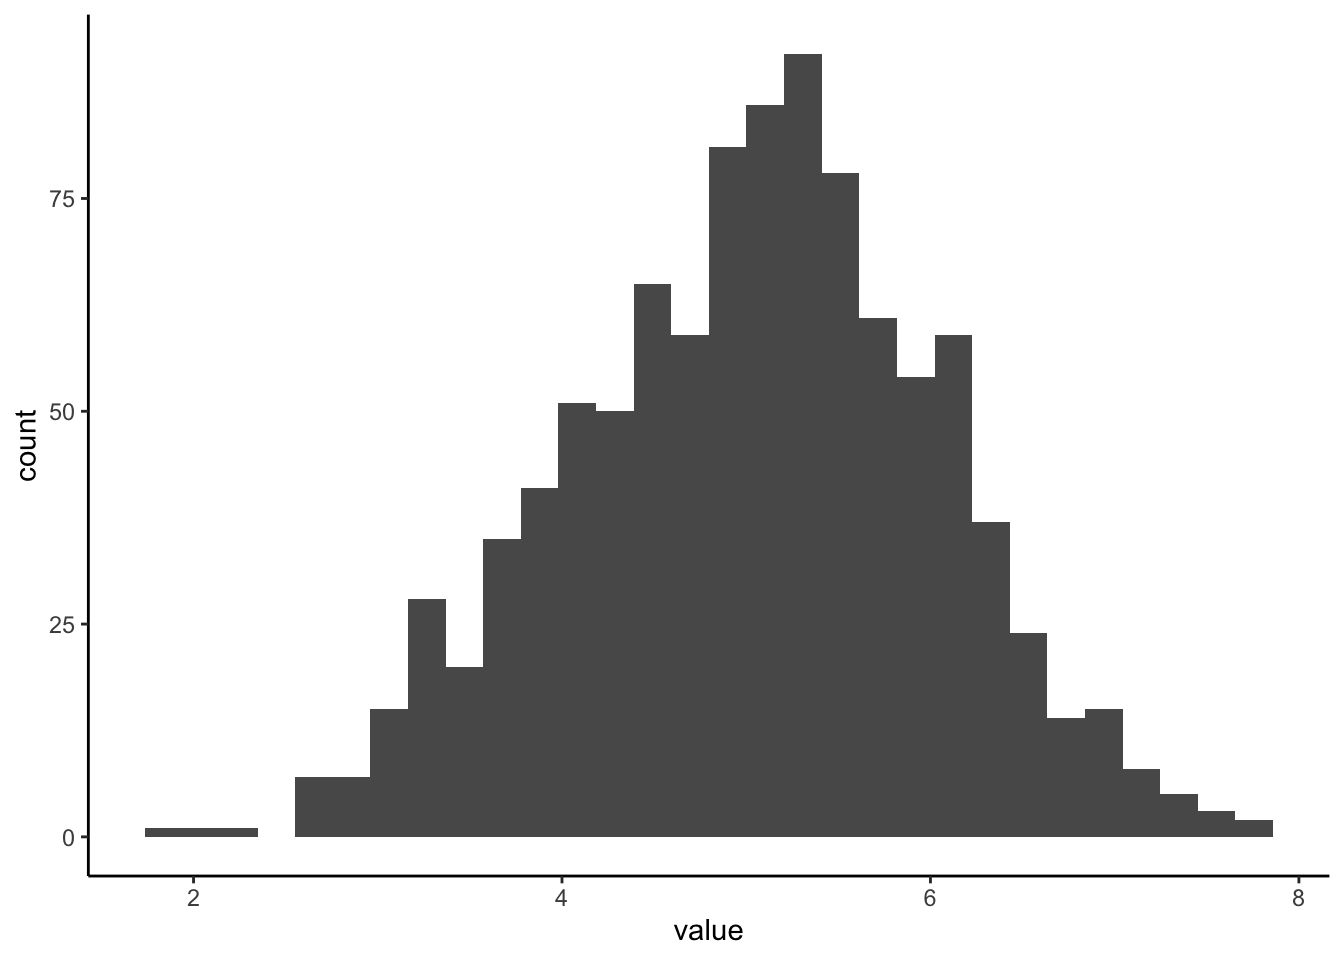
\includegraphics{Hydroinformatics_Bookdown_files/figure-latex/unnamed-chunk-42-1.pdf}

\begin{Shaded}
\begin{Highlighting}[]
\CommentTok{\#pdf}
\NormalTok{ExNorm }\SpecialCharTok{\%\textgreater{}\%}
  \FunctionTok{ggplot}\NormalTok{(}\FunctionTok{aes}\NormalTok{(value)) }\SpecialCharTok{+}
  \FunctionTok{stat\_density}\NormalTok{()}
\end{Highlighting}
\end{Shaded}

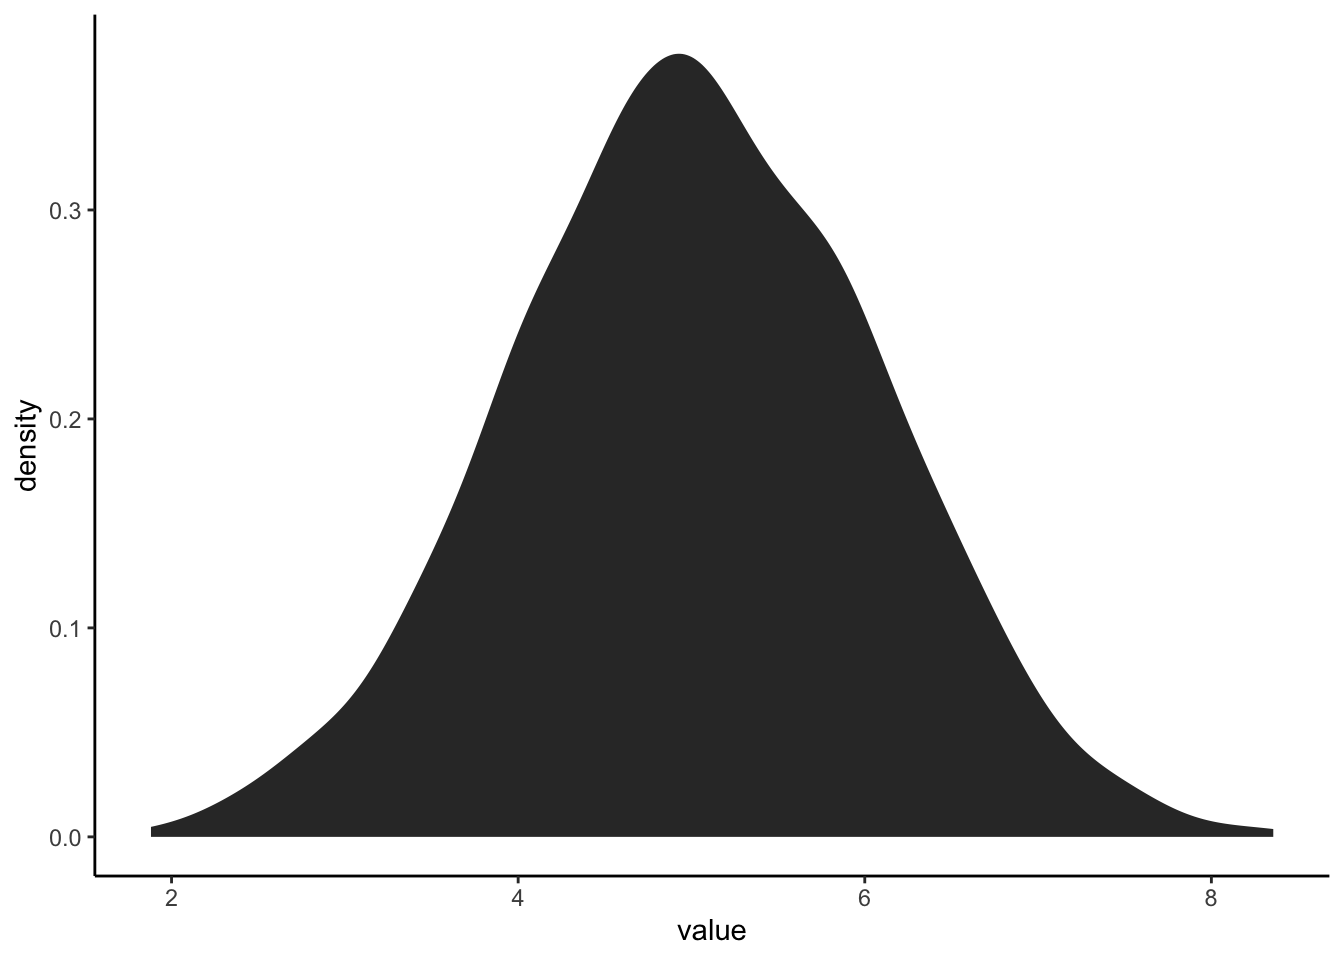
\includegraphics{Hydroinformatics_Bookdown_files/figure-latex/unnamed-chunk-42-2.pdf}

\begin{Shaded}
\begin{Highlighting}[]
\CommentTok{\#Let\textquotesingle{}s generate a plot that makes comparing these two easier}
\end{Highlighting}
\end{Shaded}

\hypertarget{stack-plots-to-compare-histogram-and-pdf}{%
\subsection{Stack plots to compare histogram and pdf}\label{stack-plots-to-compare-histogram-and-pdf}}

We will save each plot as ggplot object and then output them using the patchwork package (loaded in the setup chunk).

What is the difference between a histogram and a pdf?\\
What features of the histogram are preserved? Which are lost?

\begin{Shaded}
\begin{Highlighting}[]
\CommentTok{\#histogram}
\NormalTok{exhist }\OtherTok{\textless{}{-}}\NormalTok{ ExNorm }\SpecialCharTok{\%\textgreater{}\%}
  \FunctionTok{ggplot}\NormalTok{(}\FunctionTok{aes}\NormalTok{(value)) }\SpecialCharTok{+}
  \FunctionTok{geom\_histogram}\NormalTok{()}

\CommentTok{\#pdf}
\NormalTok{expdf }\OtherTok{\textless{}{-}}\NormalTok{ ExNorm }\SpecialCharTok{\%\textgreater{}\%}
  \FunctionTok{ggplot}\NormalTok{(}\FunctionTok{aes}\NormalTok{(value)) }\SpecialCharTok{+}
  \FunctionTok{stat\_density}\NormalTok{()}

\CommentTok{\#put the plots side by side with + or on top of each other with /}
\NormalTok{exhist}\SpecialCharTok{/}\NormalTok{expdf}
\end{Highlighting}
\end{Shaded}

\begin{verbatim}
## `stat_bin()` using `bins = 30`. Pick better value with `binwidth`.
\end{verbatim}

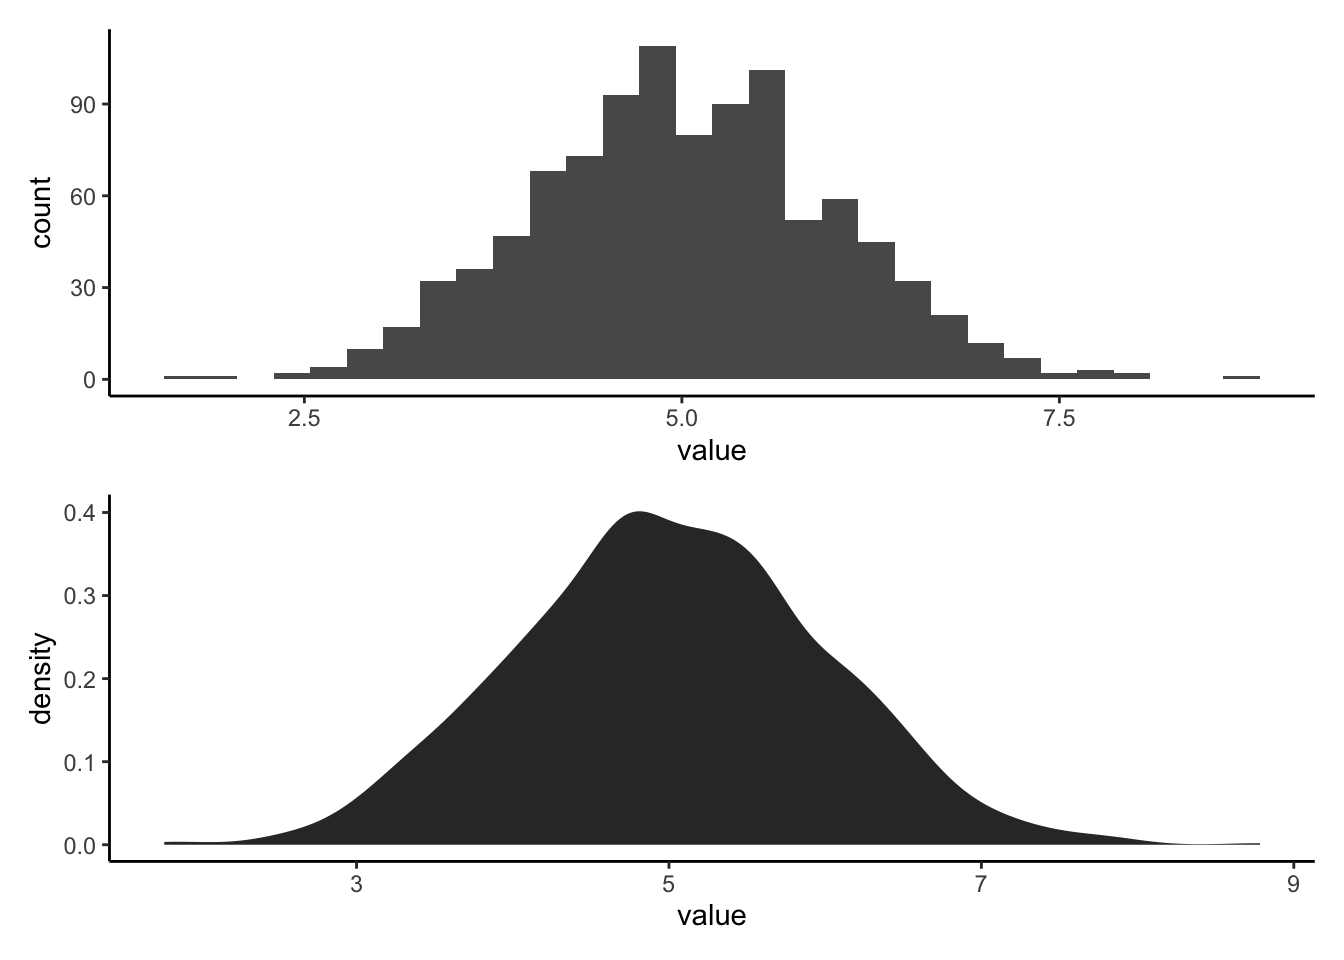
\includegraphics{Hydroinformatics_Bookdown_files/figure-latex/unnamed-chunk-43-1.pdf}

\hypertarget{what-is-the-difference-between-a-sample-and-a-population.}{%
\section{What is the difference between a sample and a population.}\label{what-is-the-difference-between-a-sample-and-a-population.}}

Simply put: a population is the thing you are trying to measure. A sample is the data you measure in an effort to measure the population. A sample is a subset of a population.

Let's write some code for an example:

We will create a POPULATION that is a large set of numbers. Think of this is as the concentration of Calcium in every bit of water in a lake. Then we will create a SAMPLE by randomly grabbing values from the POPULATION. This simulates us going around in a boat and taking grab samples in an effort to figure out the concentration of calcium in the lake.

We can then run this code a bunch of times, you'll get a different sample each time. You can also take a smaller or larger number of samples by changing ``size'' in the sample() function.

How does your sample distribution look similar or different from the population?\\
Why does the sample change every time you run it?\\
What happens as you increase or decrease the number of samples?\\
What happens if you set the number of samples to the size of the population?

\begin{Shaded}
\begin{Highlighting}[]
\NormalTok{all\_the\_water }\OtherTok{\textless{}{-}} \FunctionTok{rnorm}\NormalTok{(}\DecValTok{10000}\NormalTok{, }\AttributeTok{mean =} \DecValTok{6}\NormalTok{) }\SpecialCharTok{\%\textgreater{}\%} \FunctionTok{as\_tibble}\NormalTok{()}

\NormalTok{sample\_of\_water }\OtherTok{\textless{}{-}} \FunctionTok{sample}\NormalTok{(all\_the\_water}\SpecialCharTok{$}\NormalTok{value, }\AttributeTok{size =} \DecValTok{100}\NormalTok{, }\AttributeTok{replace =} \ConstantTok{FALSE}\NormalTok{) }\SpecialCharTok{\%\textgreater{}\%} \FunctionTok{as\_tibble}\NormalTok{()}

\NormalTok{population\_hist }\OtherTok{\textless{}{-}}\NormalTok{ all\_the\_water }\SpecialCharTok{\%\textgreater{}\%}
  \FunctionTok{ggplot}\NormalTok{(}\FunctionTok{aes}\NormalTok{(value))}\SpecialCharTok{+}
  \FunctionTok{geom\_histogram}\NormalTok{()}\SpecialCharTok{+}
  \FunctionTok{ggtitle}\NormalTok{(}\StringTok{"Population: All the water in the lake"}\NormalTok{)}

\NormalTok{sample\_hist }\OtherTok{\textless{}{-}}\NormalTok{ sample\_of\_water }\SpecialCharTok{\%\textgreater{}\%}
  \FunctionTok{ggplot}\NormalTok{(}\FunctionTok{aes}\NormalTok{(value))}\SpecialCharTok{+}
  \FunctionTok{geom\_histogram}\NormalTok{()}\SpecialCharTok{+}
  \FunctionTok{ggtitle}\NormalTok{(}\StringTok{"Your sample of the lake"}\NormalTok{)}

\NormalTok{population\_hist }\SpecialCharTok{+}\NormalTok{ sample\_hist}
\end{Highlighting}
\end{Shaded}

\begin{verbatim}
## `stat_bin()` using `bins = 30`. Pick better value with `binwidth`.
## `stat_bin()` using `bins = 30`. Pick better value with `binwidth`.
\end{verbatim}

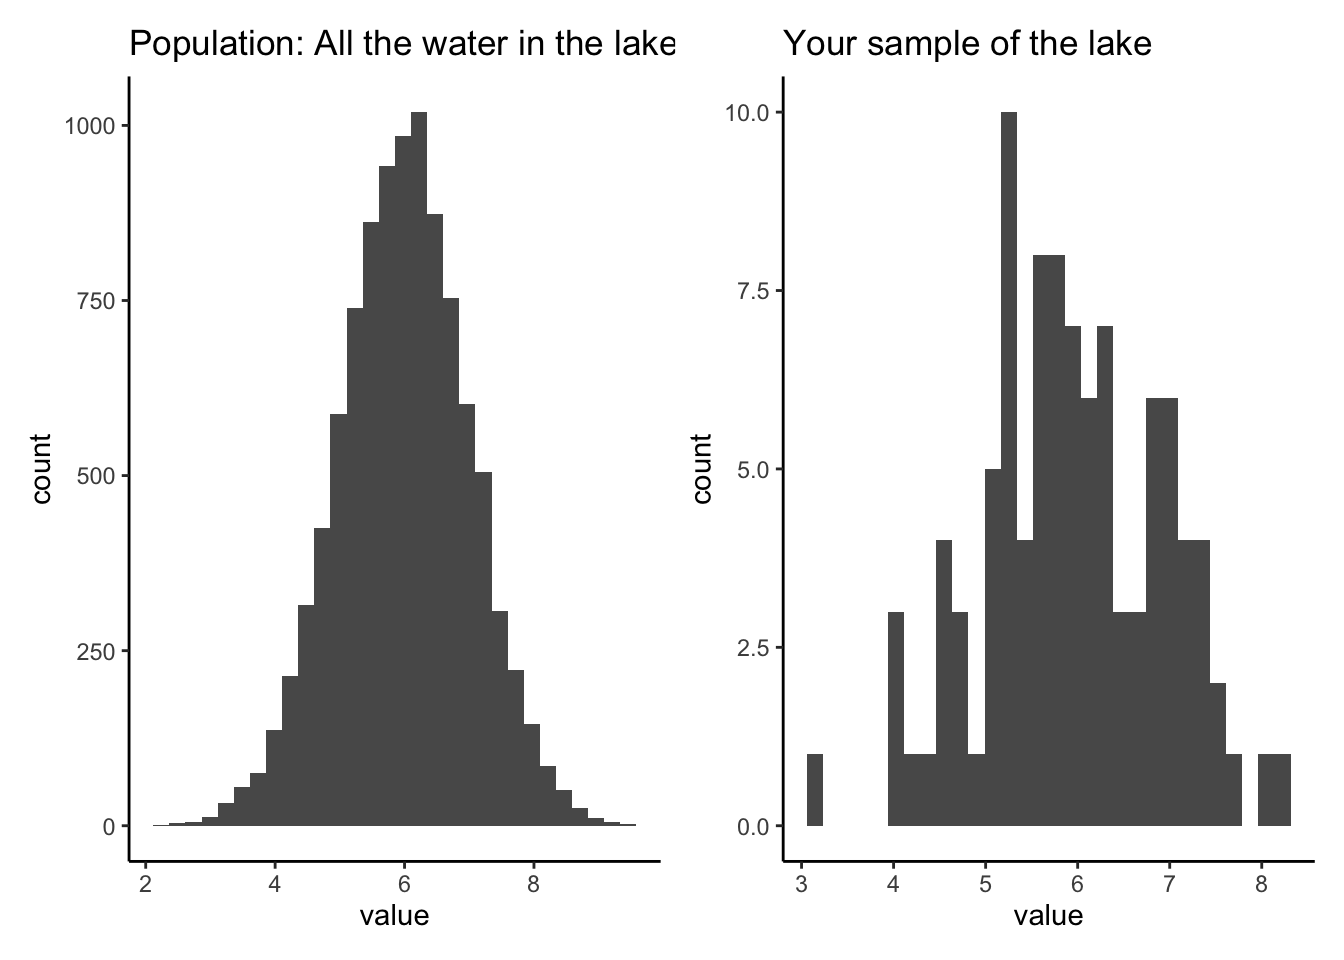
\includegraphics{Hydroinformatics_Bookdown_files/figure-latex/unnamed-chunk-44-1.pdf}

\hypertarget{measuring-our-sample-distribution-central-tendency.}{%
\section{Measuring our sample distribution: central tendency.}\label{measuring-our-sample-distribution-central-tendency.}}

When we take a sample of a population, there are a few things we will want to measure about the distribution of values: where is the middle, how variable is it, and is it skewed to one side or another?

The first of these, ``where is the middle?'' is addressed with measures of central tendency. We will discuss three possible ways to measure this. The mean, median, and weighted mean.

To explain the importance of choosing between the mean and median, we will first import some discharge data. Read in the PINE discharge data.

\begin{Shaded}
\begin{Highlighting}[]
\NormalTok{pineQ }\OtherTok{\textless{}{-}} \FunctionTok{read\_csv}\NormalTok{(}\StringTok{"PINE\_Jan{-}Mar\_2010.csv"}\NormalTok{)}
\end{Highlighting}
\end{Shaded}

\begin{verbatim}
## 
## -- Column specification --------------------------------------------------------
## cols(
##   StationID = col_character(),
##   cfs = col_double(),
##   surrogate = col_character(),
##   datetime = col_datetime(format = ""),
##   year = col_double(),
##   quarter = col_double(),
##   month = col_double(),
##   day = col_double()
## )
\end{verbatim}

To find the mean (average), you just sum up all the values in your sample and divide by the number of values.

To find the median, you put the values IN ORDER, and choose the middle value. The middle value is the one where there are the same number of values higher than that value as there are values lower than it.

Because it uses the order of the values rather than just the values themselves, the median is resistant to skewed distributions. This means it is less effected by very large or very small values compared to most values in the sample data.

Let's look at our normal distribution from earlier (ExNorm) compared to the Pine watershed discharge (pineQ)

Note that distributions like pineQ, that are positively skewed, are very common in environmental data.

\begin{Shaded}
\begin{Highlighting}[]
\CommentTok{\#Calculate mean and median for cfs in pineQ and values in ExNorm}
\NormalTok{pineMean }\OtherTok{\textless{}{-}} \FunctionTok{mean}\NormalTok{(pineQ}\SpecialCharTok{$}\NormalTok{cfs)}
\NormalTok{pineMedian }\OtherTok{\textless{}{-}} \FunctionTok{median}\NormalTok{(pineQ}\SpecialCharTok{$}\NormalTok{cfs)}

\NormalTok{xmean }\OtherTok{\textless{}{-}} \FunctionTok{mean}\NormalTok{(ExNorm}\SpecialCharTok{$}\NormalTok{value)}
\NormalTok{xmedian }\OtherTok{\textless{}{-}} \FunctionTok{median}\NormalTok{(ExNorm}\SpecialCharTok{$}\NormalTok{value)}

\CommentTok{\#plot mean and median on the ExNorm distribution}
\NormalTok{Ex }\OtherTok{\textless{}{-}}\NormalTok{ ExNorm }\SpecialCharTok{\%\textgreater{}\%} \FunctionTok{ggplot}\NormalTok{(}\FunctionTok{aes}\NormalTok{(value)) }\SpecialCharTok{+}
  \FunctionTok{geom\_histogram}\NormalTok{()}\SpecialCharTok{+}
  \FunctionTok{geom\_vline}\NormalTok{(}\AttributeTok{xintercept =}\NormalTok{ xmean, }\AttributeTok{color =} \StringTok{"red"}\NormalTok{)}\SpecialCharTok{+}
  \FunctionTok{geom\_vline}\NormalTok{(}\AttributeTok{xintercept =}\NormalTok{ xmedian, }\AttributeTok{color =} \StringTok{"blue"}\NormalTok{)}

\CommentTok{\#plot mean and median on the pineQ discharge histogram}
\NormalTok{PineP }\OtherTok{\textless{}{-}}\NormalTok{ pineQ }\SpecialCharTok{\%\textgreater{}\%} \FunctionTok{ggplot}\NormalTok{(}\FunctionTok{aes}\NormalTok{(cfs)) }\SpecialCharTok{+}
  \FunctionTok{geom\_histogram}\NormalTok{()}\SpecialCharTok{+}
  \FunctionTok{geom\_vline}\NormalTok{(}\AttributeTok{xintercept =}\NormalTok{ pineMean, }\AttributeTok{color =} \StringTok{"red"}\NormalTok{)}\SpecialCharTok{+}
  \FunctionTok{geom\_vline}\NormalTok{(}\AttributeTok{xintercept =}\NormalTok{ pineMedian, }\AttributeTok{color =} \StringTok{"blue"}\NormalTok{)}

\NormalTok{Ex }\SpecialCharTok{/}\NormalTok{ PineP  }
\end{Highlighting}
\end{Shaded}

\begin{verbatim}
## `stat_bin()` using `bins = 30`. Pick better value with `binwidth`.
## `stat_bin()` using `bins = 30`. Pick better value with `binwidth`.
\end{verbatim}

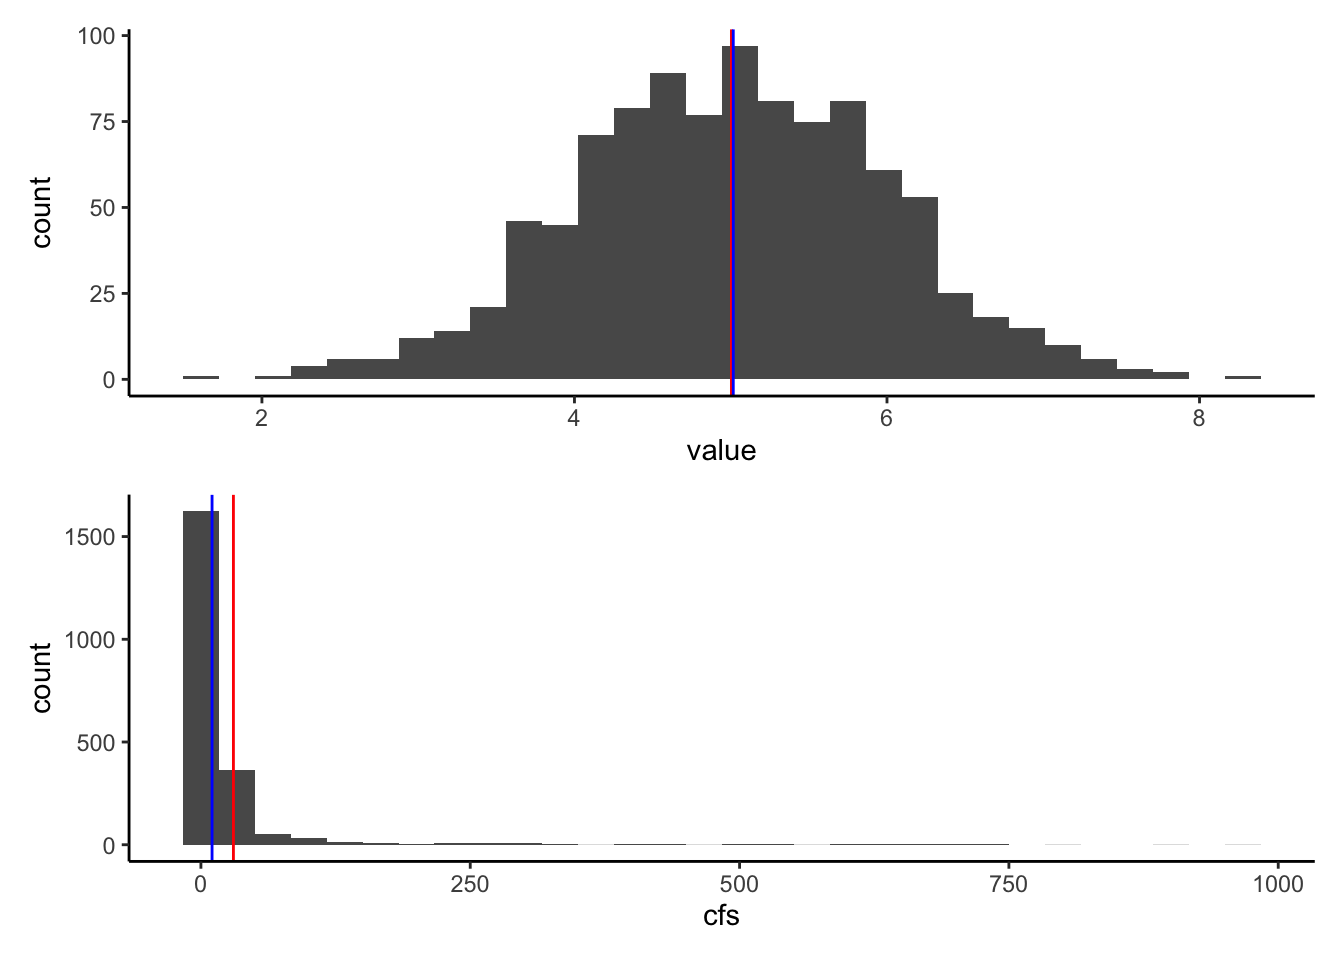
\includegraphics{Hydroinformatics_Bookdown_files/figure-latex/unnamed-chunk-46-1.pdf}

\hypertarget{so-whats-a-weighted-average}{%
\subsection{So what's a weighted average?}\label{so-whats-a-weighted-average}}

When you compute a standard mean or median, you are giving equal weight to each measurement. Adding up all the values in a sample and dividing by the number of samples is the same as multiplying each value by 1/\# of samples. For instance if you had ten samples, to calculate the mean you would add them up and divide by 10. This is the same as multiplying each value by 1/10 and then adding them up. Each value is equally weighted at 1/10.

There are certain situations in which this is not the ideal way to calculate an average. A common one in hydrology is that you have samples that are supposed to represent different portions of an area. One sample may be taken to measure a forest type that takes up 100 ha of a watershed while another sample represents a forest type that only takes up 4 ha. You may not want to simply average those values!

Another example is precipitation gages. In the image below, you see there are 5 rain gages. To get a precipitation number for the watershed, we could just average them, or we could assume they represent an area of the watershed and then weight their values by the area they represent. One method of designating the areas is by using Theissen polygons (the middle watershed). Another method of weighting is isohyetal contours, but we won't worry about that for now!

In the weighted situation, we find the average by multiplying each precipitation values by the proportion of the watershed it represents, shown by the Thiessen polygons, and then add them all together. Let's do an example.

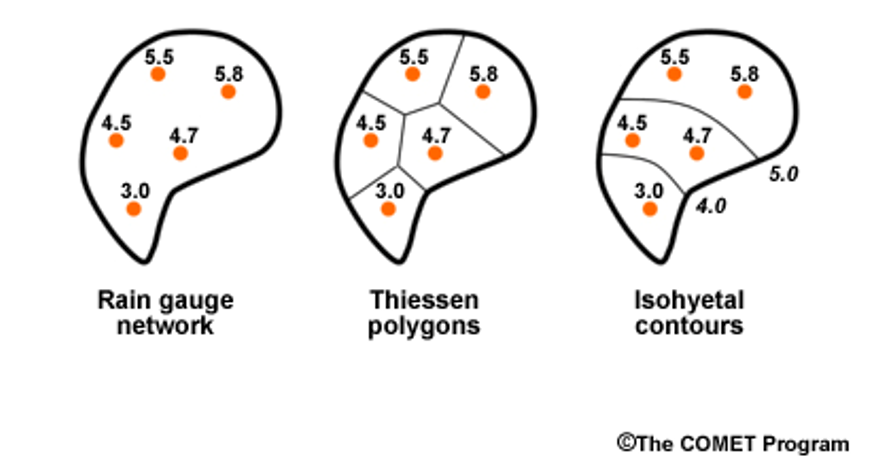
\includegraphics{images/theissen.png}source: \url{https://edx.hydrolearn.org/assets/courseware/v1/e5dc65098f1e8c5faacae0e171e28ccf/asset-v1:HydroLearn+HydroLearn401+2019_S2+type@asset+block/l2_image004.png}

The precip values for the watershed above are 4.5, 5.5, 5.8, 4.7, and 3.0

We will assume the proportions of the watershed that each gauge represents are 0.20, 0.15, 0.40, 0.15, 0.10, respectively (or 20\%, 15\%, 40\%, 15\%, 10\%)

Write some code to compute the regular mean precip from the values, and then the weighted mean.

\begin{Shaded}
\begin{Highlighting}[]
\NormalTok{precip }\OtherTok{\textless{}{-}} \FunctionTok{c}\NormalTok{(}\FloatTok{4.5}\NormalTok{, }\FloatTok{5.5}\NormalTok{, }\FloatTok{5.8}\NormalTok{, }\FloatTok{4.7}\NormalTok{, }\FloatTok{3.0}\NormalTok{)}
\NormalTok{weights }\OtherTok{\textless{}{-}} \FunctionTok{c}\NormalTok{(}\FloatTok{0.2}\NormalTok{, }\FloatTok{0.15}\NormalTok{, }\FloatTok{0.4}\NormalTok{, }\FloatTok{0.15}\NormalTok{, }\FloatTok{0.1}\NormalTok{)}

\FunctionTok{mean}\NormalTok{(precip)}
\end{Highlighting}
\end{Shaded}

\begin{verbatim}
## [1] 4.7
\end{verbatim}

\begin{Shaded}
\begin{Highlighting}[]
\FunctionTok{sum}\NormalTok{(precip }\SpecialCharTok{*}\NormalTok{ weights)}
\end{Highlighting}
\end{Shaded}

\begin{verbatim}
## [1] 5.05
\end{verbatim}

\hypertarget{measures-of-variability}{%
\section{Measures of variability}\label{measures-of-variability}}

Measures of variability allow us to measure the width of our sample data histogram or pdf. If all the values in our sample are close together, we would have small measures of variability, and a pointy pdf/histogram. If they vary more, we would have larger measures of variability and a broad pdf/histogram.

We will explore four measures of variability:

\hypertarget{variance}{%
\subsubsection{Variance:}\label{variance}}

Sum of the squared difference of each value from the mean divided by the number of samples minus 1. var()

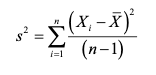
\includegraphics{images/Screen Shot 2021-01-25 at 10.29.45 AM.png}(\url{https://pubs.usgs.gov/tm/04/a03/tm4a3.pdf}) source: \url{https://pubs.usgs.gov/tm/04/a03/tm4a3.pdf}

\hypertarget{standard-deviation}{%
\subsubsection{Standard deviation:}\label{standard-deviation}}

The square root of the variance sd()

**Both variance and standard deviation are sensitive to outliers.

\hypertarget{cv-coefficient-of-variation}{%
\subsubsection{CV: Coefficient of Variation}\label{cv-coefficient-of-variation}}

CV is simply the standard deviation divided by the mean of the data. Because you divide by the mean, CV is dimensionless. This allows you to use it to compare the variation in samples with very different magnitudes.

\hypertarget{iqr-interquartile-range}{%
\subsubsection{IQR: Interquartile Range}\label{iqr-interquartile-range}}

IQR is resistant to outliers because it works like a median. It measures the range of the middle 50\% of the data in your distribution. So the IQR is the difference between the value between the 75th and 25th percentiles of your data, where the 75th percentile means 75\% of the data is BELOW that value and the 25th percentile means 25\% is below that value. Using the same vocabulary, the median is the same as the 50th percentile of the data.

If you ask R for the QUANTILES of your sample data, it will give you the values at which 0\%, 25\%, 50\%, 75\%, and 100\% of the data are below. These are the 1,2,3,4, and 5th quantiles. Therefore, the IQR is the difference between the 4th and 2nd quantile.

Okay, code time.

First, let's explore how changing the variability of a distribution changes the shape of it's distribution. Create a plot a random normal distribution using rnorm() and set sd to different numbers. Make the mean of the distribution 0, the sample size 300, and the standard deviation 1 to start. Then increase the standard deviation incrementally to 10 and see what happens. Make the limits of the x axis on the plot -30 to 30.

\begin{Shaded}
\begin{Highlighting}[]
\FunctionTok{rnorm}\NormalTok{(}\DecValTok{300}\NormalTok{, }\AttributeTok{mean =} \DecValTok{0}\NormalTok{, }\AttributeTok{sd =} \DecValTok{1}\NormalTok{) }\SpecialCharTok{\%\textgreater{}\%}\NormalTok{ as\_tibble }\SpecialCharTok{\%\textgreater{}\%}
  \FunctionTok{ggplot}\NormalTok{(}\FunctionTok{aes}\NormalTok{(value))}\SpecialCharTok{+}
  \FunctionTok{stat\_density}\NormalTok{()}\SpecialCharTok{+}
  \FunctionTok{xlim}\NormalTok{(}\FunctionTok{c}\NormalTok{(}\SpecialCharTok{{-}}\DecValTok{30}\NormalTok{,}\DecValTok{30}\NormalTok{))}
\end{Highlighting}
\end{Shaded}

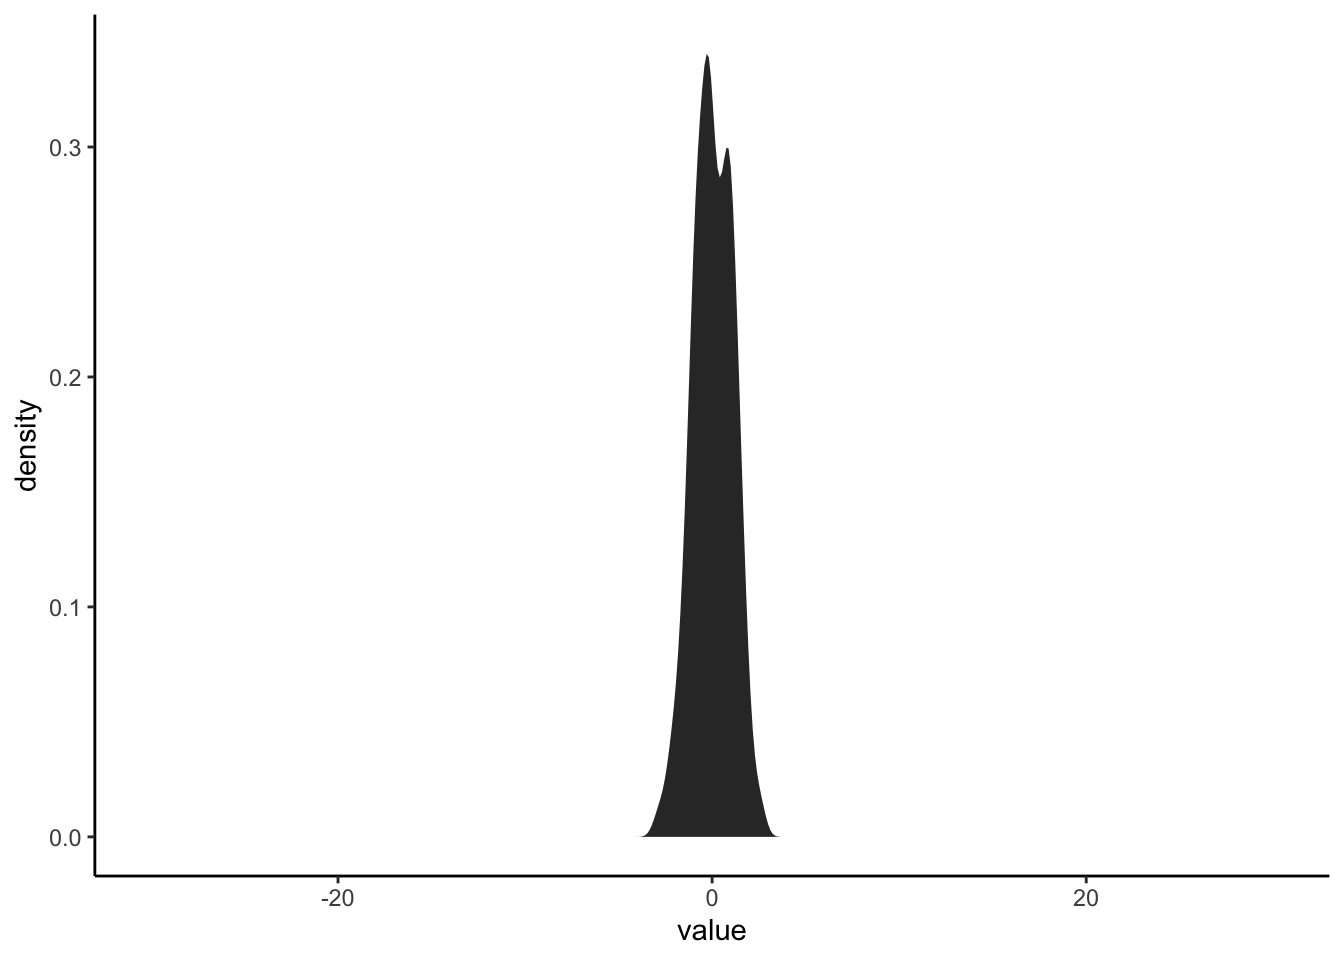
\includegraphics{Hydroinformatics_Bookdown_files/figure-latex/unnamed-chunk-48-1.pdf}

Now let's calculate the standard deviation, variance, coefficient of variation, and IQR of the Pine discharge data.

\begin{Shaded}
\begin{Highlighting}[]
\CommentTok{\#standard deviation}
\FunctionTok{sd}\NormalTok{(pineQ}\SpecialCharTok{$}\NormalTok{cfs)}
\end{Highlighting}
\end{Shaded}

\begin{verbatim}
## [1] 84.47625
\end{verbatim}

\begin{Shaded}
\begin{Highlighting}[]
\CommentTok{\#variance}
\FunctionTok{var}\NormalTok{(pineQ}\SpecialCharTok{$}\NormalTok{cfs)}
\end{Highlighting}
\end{Shaded}

\begin{verbatim}
## [1] 7136.237
\end{verbatim}

\begin{Shaded}
\begin{Highlighting}[]
\CommentTok{\#coefficient of variation}
\FunctionTok{sd}\NormalTok{(pineQ}\SpecialCharTok{$}\NormalTok{cfs)}\SpecialCharTok{/}\FunctionTok{mean}\NormalTok{(pineQ}\SpecialCharTok{$}\NormalTok{cfs)}
\end{Highlighting}
\end{Shaded}

\begin{verbatim}
## [1] 2.800221
\end{verbatim}

\begin{Shaded}
\begin{Highlighting}[]
\CommentTok{\#IQR using the IQR funciton}
\FunctionTok{IQR}\NormalTok{(pineQ}\SpecialCharTok{$}\NormalTok{cfs)}
\end{Highlighting}
\end{Shaded}

\begin{verbatim}
## [1] 8.1325
\end{verbatim}

\begin{Shaded}
\begin{Highlighting}[]
\CommentTok{\#IQR using the quantile function}
\NormalTok{quants }\OtherTok{\textless{}{-}} \FunctionTok{quantile}\NormalTok{(pineQ}\SpecialCharTok{$}\NormalTok{cfs)}
\NormalTok{quants[}\DecValTok{4}\NormalTok{] }\SpecialCharTok{{-}}\NormalTok{ quants[}\DecValTok{2}\NormalTok{]}
\end{Highlighting}
\end{Shaded}

\begin{verbatim}
##    75% 
## 8.1325
\end{verbatim}

\hypertarget{what-about-how-lopsided-the-distribution-is}{%
\subsubsection{What about how lopsided the distribution is?}\label{what-about-how-lopsided-the-distribution-is}}

There are several ways to measure this as well, but we are just going to look at one: The Quartile skew. The quartile skew is the difference between the upper quartiles (50th-75th) and the lower quartiles (25th-50th) divided by the IQR (75th-25th).

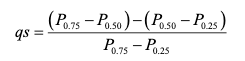
\includegraphics{images/Screen Shot 2021-01-25 at 11.27.14 AM.png} source: \url{https://pubs.usgs.gov/tm/04/a03/tm4a3.pdf}

Let's look at the quartile skew of the two distributions we've been measuring. Calculate it for the pineQ discharge data and the random normal distribution we generated.

Which one is more skewed?

\begin{Shaded}
\begin{Highlighting}[]
\NormalTok{quantsP }\OtherTok{\textless{}{-}} \FunctionTok{quantile}\NormalTok{(pineQ}\SpecialCharTok{$}\NormalTok{cfs)}

\NormalTok{((quantsP[}\DecValTok{3}\NormalTok{]}\SpecialCharTok{{-}}\NormalTok{quantsP[}\DecValTok{2}\NormalTok{]) }\SpecialCharTok{{-}}\NormalTok{ (quantsP[}\DecValTok{2}\NormalTok{] }\SpecialCharTok{{-}}\NormalTok{ quantsP[}\DecValTok{1}\NormalTok{])) }\SpecialCharTok{/}\NormalTok{ quantsP[}\DecValTok{3}\NormalTok{] }\SpecialCharTok{{-}}\NormalTok{ quantsP[}\DecValTok{1}\NormalTok{]}
\end{Highlighting}
\end{Shaded}

\begin{verbatim}
##       50% 
## -4.837233
\end{verbatim}

\begin{Shaded}
\begin{Highlighting}[]
\NormalTok{quantsX }\OtherTok{\textless{}{-}} \FunctionTok{quantile}\NormalTok{(ExNorm}\SpecialCharTok{$}\NormalTok{value)}

\NormalTok{((quantsX[}\DecValTok{3}\NormalTok{]}\SpecialCharTok{{-}}\NormalTok{quantsX[}\DecValTok{2}\NormalTok{]) }\SpecialCharTok{{-}}\NormalTok{ (quantsX[}\DecValTok{2}\NormalTok{] }\SpecialCharTok{{-}}\NormalTok{ quantsX[}\DecValTok{1}\NormalTok{])) }\SpecialCharTok{/}\NormalTok{ quantsX[}\DecValTok{3}\NormalTok{] }\SpecialCharTok{{-}}\NormalTok{ quantsX[}\DecValTok{1}\NormalTok{]}
\end{Highlighting}
\end{Shaded}

\begin{verbatim}
##       50% 
## -2.106285
\end{verbatim}

\hypertarget{what-is-a-normal-distribution-and-how-can-we-determine-if-we-have-one}{%
\section{What is a normal distribution and how can we determine if we have one?}\label{what-is-a-normal-distribution-and-how-can-we-determine-if-we-have-one}}

The distribution we generated with rnorm() is a normal distribution. The distribution of pineQ discharge is not normal. Now that we've looked at different ways to characterize distributions, we have the vocabulary to describe why.

\textbf{Normal distributions:}

\begin{itemize}
\tightlist
\item
  mean = median, half values to the right, half to the left
\item
  symmetric (not skewed)
\item
  single peak
\end{itemize}

Many statistical tests require that the distribution of the data you put into them is normally distributed. BE CAREFUL! There are also tests that use ranked data. Similar to how the median is resistant to outliers, these rank-based tests are resistant to non-normal data. Two popular ones are Kruskal-Wallis and Wilcoxon rank-sum.

But how far off can you be before you don't consider a distribution normal? Seems like a judgement call!

R to the rescue! There is a built in test for normality called shapiro.test(), which performs the Shapiro-Wilk test of normality. The hypothesis this test tests is ``The distribution is normal.'' So if this function returns a p-value less than 0.05, you reject that hypothesis and your function is NOT normal.

You can also make a quantile-quantile plot. A straight line on this plot indicates a normal distribution, a non-straight line indicates it is not normal.

\begin{Shaded}
\begin{Highlighting}[]
\FunctionTok{shapiro.test}\NormalTok{(pineQ}\SpecialCharTok{$}\NormalTok{cfs)}
\end{Highlighting}
\end{Shaded}

\begin{verbatim}
## 
##  Shapiro-Wilk normality test
## 
## data:  pineQ$cfs
## W = 0.27155, p-value < 2.2e-16
\end{verbatim}

\begin{Shaded}
\begin{Highlighting}[]
\FunctionTok{qqnorm}\NormalTok{(pineQ}\SpecialCharTok{$}\NormalTok{cfs)}
\end{Highlighting}
\end{Shaded}

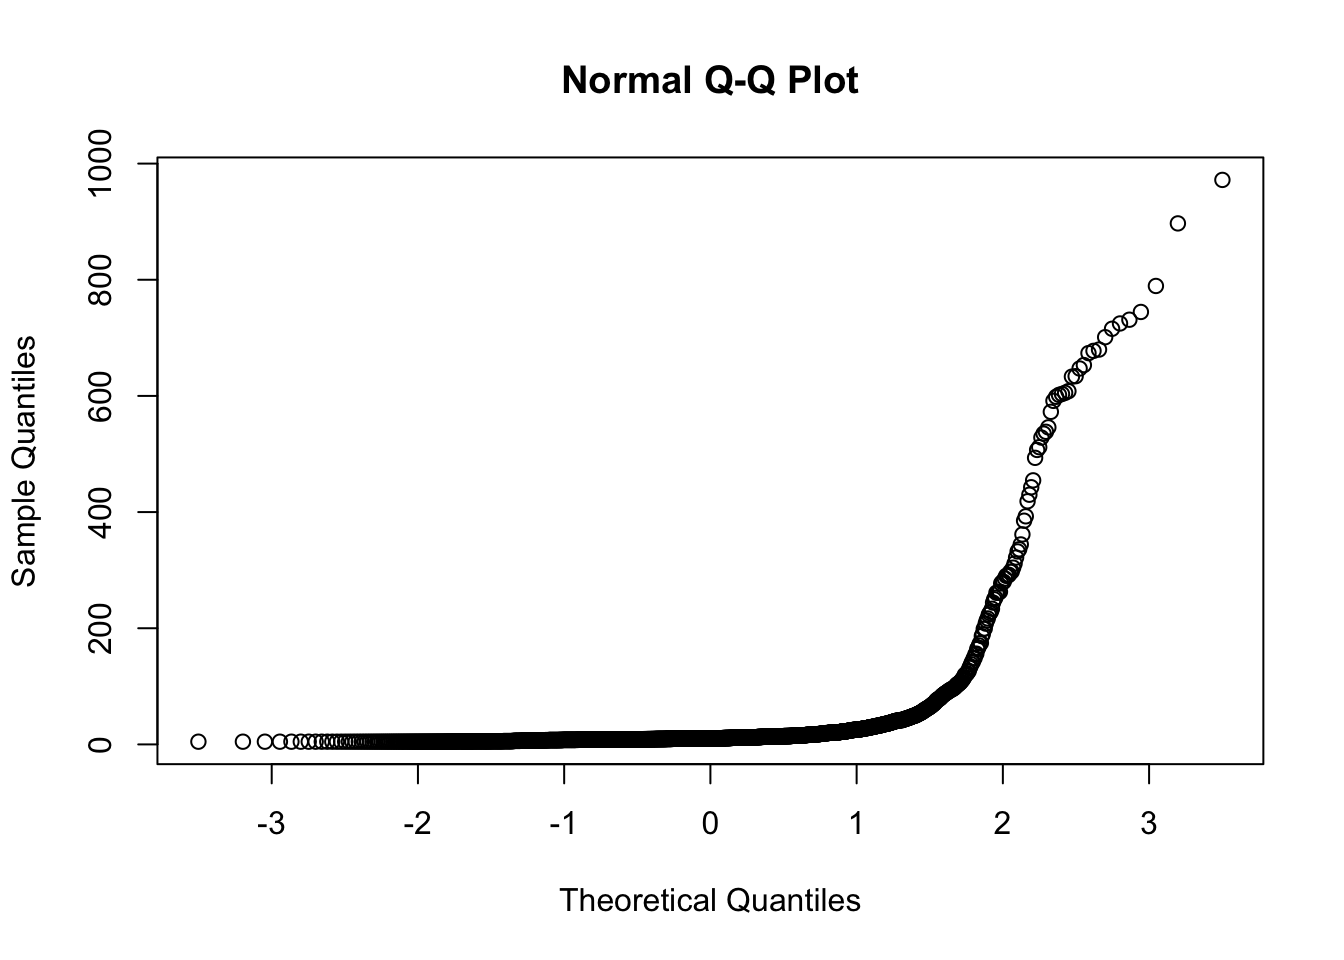
\includegraphics{Hydroinformatics_Bookdown_files/figure-latex/unnamed-chunk-51-1.pdf}

\hypertarget{statsactivity}{%
\chapter{ACTIVITY Intro Stats}\label{statsactivity}}

Get this document at the template repository on github: \url{https://github.com/VT-Hydroinformatics/5-Intro-Stats-Activity}

Address each of the questions in the code chunk below and/or by typing outside the chunk (for written answers).

\hypertarget{problem-1-1}{%
\section{Problem 1}\label{problem-1-1}}

Load the tidyverse and patchwork libraries and read in the Flashy and Pine datasets.

\hypertarget{problem-2-1}{%
\section{Problem 2}\label{problem-2-1}}

Using the flashy dataset, make a pdf of the average basin rainfall (PPTAVG\_BASIN) for the NorthEast AGGECOREGION. On that pdf, add vertical lines showing the mean, median, standard deviation, and IQR. Make each a different color and note which is which in a typed answer below this question. (or if you want an extra challenged, make a custom legend that shows this)

\hypertarget{problem-3-1}{%
\section{Problem 3}\label{problem-3-1}}

Perform a Shapiro-Wilk test for normality on the data from question 2. Using the results from that test and the plot and stats from question 2, discuss whether or not the distribution is normal.

\hypertarget{problem-4-1}{%
\section{Problem 4}\label{problem-4-1}}

Make a plot that shows the distribution of the data from the PINE watershed and the NFDR watershed (two pdfs on the same plot). Log the x axis.

\hypertarget{problem-5-1}{%
\section{Problem 5}\label{problem-5-1}}

You want to compare how variable the discharge is in each of the watersheds in question 4. Which measure of spread would you use and why? If you wanted to measure the central tendency which measure would you use and why?

\hypertarget{problem-6-1}{%
\section{Problem 6}\label{problem-6-1}}

Compute 3 measures of spread and 2 measures of central tendency for the PINE and NFDR watershed. (hint: use group\_by() and summarize()) Be sure your code outputs the result. Which watershed has higher flow? Which one has more variable flow? How do you know?

\hypertarget{getdata}{%
\chapter{Joins, Pivots, and USGS dataRetrieval}\label{getdata}}

Get this document and a version with empty code chunks at the template repository on github: \url{https://github.com/VT-Hydroinformatics/6-Get-Format-Plot-HydroData}

Readings: Introduction to the dataRetrieval package \url{https://cran.r-project.org/web/packages/dataRetrieval/vignettes/dataRetrieval.html}

Chapter 12 \& 13 of R for Data Science \url{https://r4ds.had.co.nz/tidy-data.html}

\hypertarget{goals-for-today}{%
\section{Goals for today}\label{goals-for-today}}

\begin{itemize}
\tightlist
\item
  Get familiar with the dataRetrieval package
\item
  Intro to joins
\item
  Learn about long vs.~wide data and how to change between them
\end{itemize}

Prep question: How would you get data from the USGS (non-R)?

Install the dataRetrieval package. Load it and the tidyverse.

\begin{Shaded}
\begin{Highlighting}[]
\CommentTok{\#install.packages("dataRetrieval")}
\FunctionTok{library}\NormalTok{(dataRetrieval)}
\end{Highlighting}
\end{Shaded}

\begin{verbatim}
## Warning: package 'dataRetrieval' was built under R version 3.6.2
\end{verbatim}

\begin{Shaded}
\begin{Highlighting}[]
\FunctionTok{library}\NormalTok{(tidyverse)}
\FunctionTok{library}\NormalTok{(lubridate)}
\end{Highlighting}
\end{Shaded}

\begin{verbatim}
## Warning: package 'lubridate' was built under R version 3.6.2
\end{verbatim}

\hypertarget{exploring-what-dataretrieval-can-do.}{%
\section{Exploring what dataRetrieval can do.}\label{exploring-what-dataretrieval-can-do.}}

Think about the dataRetrieval as a way to interact with same public data you can access through waterdata.usgs.gov but without having to click on buttons and search around. It makes getting data or doing analyses with USGS data much more reproducible and fast!

To explore a few of the capabilities (NOT ALL!!) we will start with the USGS gage on the New River at Radford. The gage number is 03171000.

The documentation for the package is extremely helpful: \url{https://cran.r-project.org/web/packages/dataRetrieval/vignettes/dataRetrieval.html}

I always have to look up how to do things because the package is very specialized! This is the case with most website APIs, in my experience. It's a good argument for getting good at navigating package documentation! Basically you just look through and try to piece together the recipe for what you want to do using the examples they give in the document.

First, let's get information about the site using the readNWISsite() and whatNWISdata() functions. Try each out and see what they tell you.

Remember, all the parameter codes and site names get passed to dataRetrieval functions as characters, ao they must be in quotes.

\begin{Shaded}
\begin{Highlighting}[]
\CommentTok{\#important: note the site number gets input as a character}
\NormalTok{site }\OtherTok{\textless{}{-}} \StringTok{"03171000"}

\CommentTok{\#Information about the site}
\NormalTok{siteinfo }\OtherTok{\textless{}{-}} \FunctionTok{readNWISsite}\NormalTok{(site)}

\CommentTok{\#What data is available for the site?}
\CommentTok{\#Daily values, mean values}
\NormalTok{dataAvailable }\OtherTok{\textless{}{-}} \FunctionTok{whatNWISdata}\NormalTok{(}\AttributeTok{siteNumber =}\NormalTok{ site, }\AttributeTok{service =} \StringTok{"dv"}\NormalTok{, }\AttributeTok{statCd =} \StringTok{"00003"}\NormalTok{)}

\NormalTok{dataAvailable}
\end{Highlighting}
\end{Shaded}

\begin{verbatim}
##   agency_cd  site_no               station_nm site_tp_cd dec_lat_va dec_long_va
## 2      USGS 03171000 NEW RIVER AT RADFORD, VA         ST   37.14179   -80.56922
## 3      USGS 03171000 NEW RIVER AT RADFORD, VA         ST   37.14179   -80.56922
## 4      USGS 03171000 NEW RIVER AT RADFORD, VA         ST   37.14179   -80.56922
##   coord_acy_cd dec_coord_datum_cd   alt_va alt_acy_va alt_datum_cd   huc_cd
## 2            U              NAD83  1711.99       0.13       NAVD88 05050001
## 3            U              NAD83  1711.99       0.13       NAVD88 05050001
## 4            U              NAD83  1711.99       0.13       NAVD88 05050001
##   data_type_cd parm_cd stat_cd  ts_id loc_web_ds medium_grp_cd parm_grp_cd
## 2           dv   00010   00003 241564         NA           wat        <NA>
## 3           dv   00060   00003 145684         NA           wat        <NA>
## 4           dv   00095   00003 145685         NA           wat        <NA>
##    srs_id access_cd begin_date   end_date count_nu
## 2 1645597         0 2006-12-20 2009-03-18      704
## 3 1645423         0 1907-10-01 2021-03-29    32687
## 4 1646694         0 2006-12-20 2008-09-29      534
\end{verbatim}

\hypertarget{joins}{%
\section{Joins}\label{joins}}

When we look at what whatNWISdata returns, we see it gives us parameter codes, but doesn't tell us what they mean. This is a common attribute of databases: you use a common identifier but then have the full information in a lookup file. In this case, the look-up information telling us what the parameter codes mean is in ``parameterCdFile'' which loads with the dataRetrieval package.

So, you could look at that and see what the parameters mean.

OR We could have R do it and add a column that tells us what the parameters mean. Enter JOINS!

Joins allow us to combine the data from two different data sets that have a column in common. At its most basic, a join looks for a matching row with the same key in both datasets (for example, a USGS gage number) and then combines the rows. So now you have all the data from both sets, matched on the key.

But you have to make some decisions: what if a key value exists in one set but not the other? Do you just drop that observation? Do you add an NA? Let's look at the different options.

Take for example the two data sets, FlowTable and SizeTable. The SiteName values are the key values and the MeanFlow and WSsize values are the data.

\begin{figure}
\centering
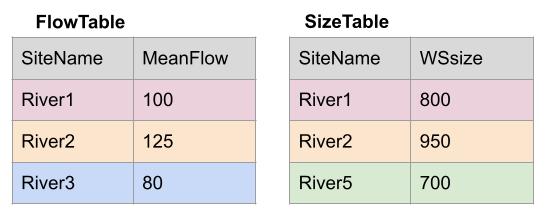
\includegraphics[width=4.16667in,height=\textheight]{images/joinsetup.png}
\caption{Join Setup}
\end{figure}

Note River1 and River2 match up, but River3 and River5 only exist in one data set or the other.

The first way to deal with this is an \textbf{INNER JOIN: inner\_join()} In an inner join, you only keep records that match. So the rows for River3 and River5 will be dropped because there is no corresponding data in the other set. See below:

\begin{figure}
\centering
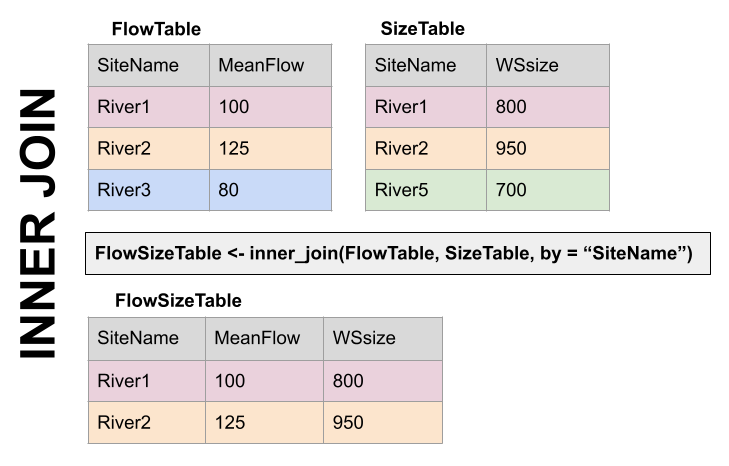
\includegraphics{images/innerjoin.png}
\caption{Inner Join}
\end{figure}

But what if you don't want to lose the values in one or the other or both?!

For instance, let's say you have a bunch of discharge data for a stream, and then chemistry grab samples. You want to join the chemistry to the discharge based on the dates and times they were taken. But when you do this, you don't want to delete all the discharge data where there is no chemistry! We need another option. Enter OUTER JOINS

\textbf{LEFT JOIN, left\_join():} Preserves all values from the LEFT data set, and pastes on the matching ones from the right. This creates NAs where there is a value on the left but not the right. (this is what you'd want to do in the discharge - chemistry example above)

\begin{figure}
\centering
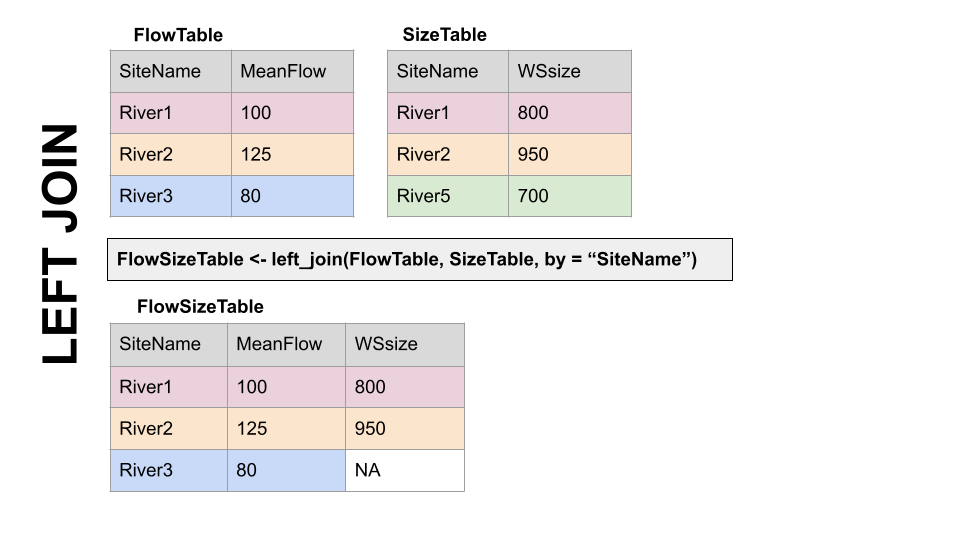
\includegraphics{images/leftjoin1.png}
\caption{Left Join}
\end{figure}

\textbf{RIGHT JOIN, right\_join():} Preserves all values from the RIGHT data set, and pastes on the matching ones from the left. This creates NAs where there is a value on the right but not the left.

\begin{figure}
\centering
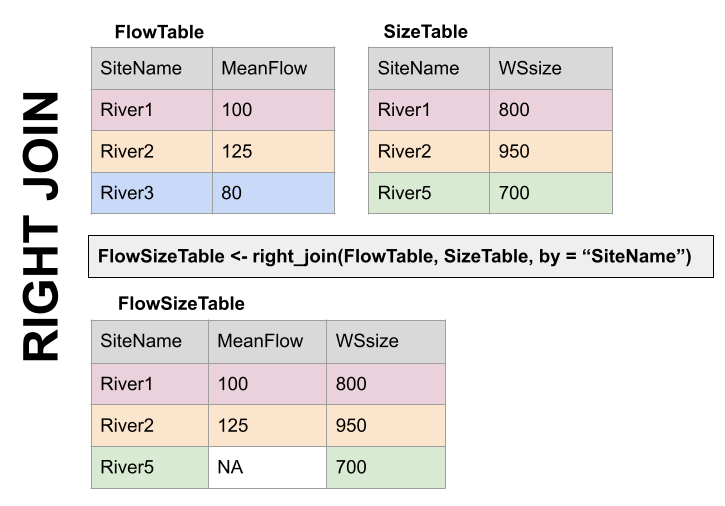
\includegraphics{images/rightjoin.png}
\caption{Right Join}
\end{figure}

\textbf{FULL JOIN, full\_join():} KEEP EVERYTHING! The hoarder of the joins. No matching record on the left? create an NA on the right! No matching value on the right? Create an NA on the left! NAs for everyone!

\begin{figure}
\centering
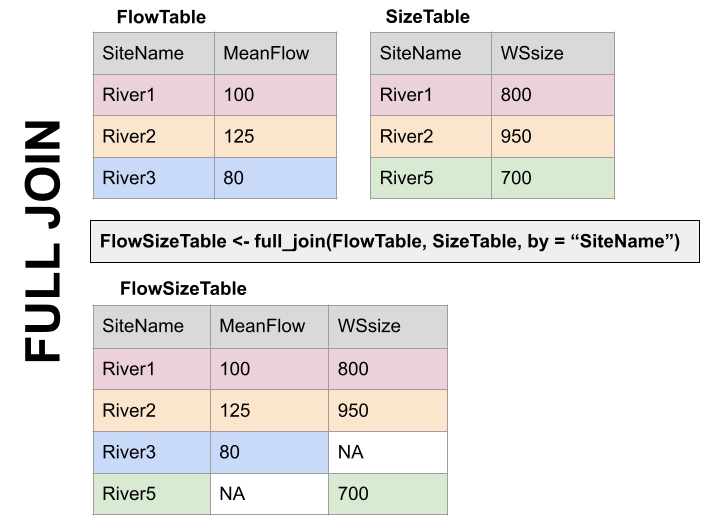
\includegraphics{images/fulljoin.png}
\caption{Full Join}
\end{figure}

When you do this in R, you use the functions identified in the descriptions with the following syntax (see example below):

\textbf{if the column is named the same in both data sets}
\textgreater{} xxx\_join(left\_tibble, right\_tibble, by = ``key\_column'')**

\textbf{if the column is named differently in both data sets}
\textgreater{} xxx\_join(left\_tibble, right\_tibble, by = c(``left\_key'' = ``right\_key'')

\begin{figure}
\centering
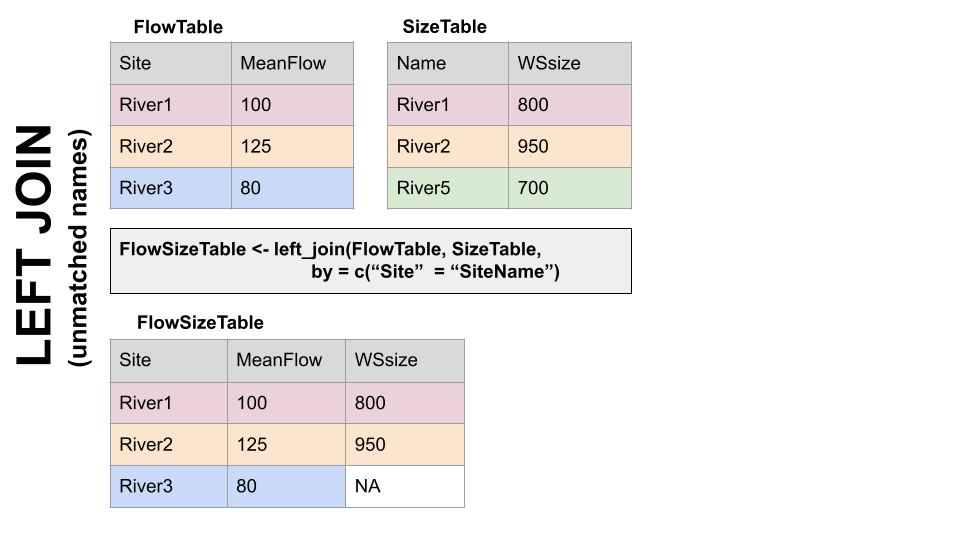
\includegraphics{images/leftjoin2.png}
\caption{Left Join Differing Col Names}
\end{figure}

Note in both of the above, when you specify which column to use as ``by'' you have to put it in quotes.

\hypertarget{join-example}{%
\section{Join example}\label{join-example}}

So in the chunk below let's get add information about the parameters in dataAvailable by joining it with the key file: parameterCdFile. The column with the parameter codes is called parm\_cd in dataAvailable and parameter\_cd in parameterCdFile

\begin{Shaded}
\begin{Highlighting}[]
\NormalTok{dataAvailable }\OtherTok{\textless{}{-}} \FunctionTok{left\_join}\NormalTok{(dataAvailable, parameterCdFile, }\AttributeTok{by =} \FunctionTok{c}\NormalTok{(}\StringTok{"parm\_cd"} \OtherTok{=} \StringTok{"parameter\_cd"}\NormalTok{))}

\NormalTok{dataAvailable}
\end{Highlighting}
\end{Shaded}

\begin{verbatim}
##   agency_cd  site_no               station_nm site_tp_cd dec_lat_va dec_long_va
## 1      USGS 03171000 NEW RIVER AT RADFORD, VA         ST   37.14179   -80.56922
## 2      USGS 03171000 NEW RIVER AT RADFORD, VA         ST   37.14179   -80.56922
## 3      USGS 03171000 NEW RIVER AT RADFORD, VA         ST   37.14179   -80.56922
##   coord_acy_cd dec_coord_datum_cd   alt_va alt_acy_va alt_datum_cd   huc_cd
## 1            U              NAD83  1711.99       0.13       NAVD88 05050001
## 2            U              NAD83  1711.99       0.13       NAVD88 05050001
## 3            U              NAD83  1711.99       0.13       NAVD88 05050001
##   data_type_cd parm_cd stat_cd  ts_id loc_web_ds medium_grp_cd parm_grp_cd
## 1           dv   00010   00003 241564         NA           wat        <NA>
## 2           dv   00060   00003 145684         NA           wat        <NA>
## 3           dv   00095   00003 145685         NA           wat        <NA>
##    srs_id access_cd begin_date   end_date count_nu parameter_group_nm
## 1 1645597         0 2006-12-20 2009-03-18      704           Physical
## 2 1645423         0 1907-10-01 2021-03-29    32687           Physical
## 3 1646694         0 2006-12-20 2008-09-29      534           Physical
##                                                                                 parameter_nm
## 1                                                        Temperature, water, degrees Celsius
## 2                                                           Discharge, cubic feet per second
## 3 Specific conductance, water, unfiltered, microsiemens per centimeter at 25 degrees Celsius
##   casrn                  srsname parameter_units
## 1  <NA>       Temperature, water           deg C
## 2  <NA> Stream flow, mean. daily           ft3/s
## 3  <NA>     Specific conductance      uS/cm @25C
\end{verbatim}

\begin{Shaded}
\begin{Highlighting}[]
\CommentTok{\#that made a lot of columns, let\textquotesingle{}s clean it up}
\NormalTok{dataAvailClean }\OtherTok{\textless{}{-}}\NormalTok{ dataAvailable }\SpecialCharTok{\%\textgreater{}\%} \FunctionTok{select}\NormalTok{(site\_no, }
\NormalTok{                                           station\_nm,}
\NormalTok{                                           parm\_cd, }
\NormalTok{                                           srsname, }
\NormalTok{                                           parameter\_units,}
\NormalTok{                                           begin\_date, }
\NormalTok{                                           end\_date)}

\NormalTok{dataAvailClean}
\end{Highlighting}
\end{Shaded}

\begin{verbatim}
##    site_no               station_nm parm_cd                  srsname
## 1 03171000 NEW RIVER AT RADFORD, VA   00010       Temperature, water
## 2 03171000 NEW RIVER AT RADFORD, VA   00060 Stream flow, mean. daily
## 3 03171000 NEW RIVER AT RADFORD, VA   00095     Specific conductance
##   parameter_units begin_date   end_date
## 1           deg C 2006-12-20 2009-03-18
## 2           ft3/s 1907-10-01 2021-03-29
## 3      uS/cm @25C 2006-12-20 2008-09-29
\end{verbatim}

\hypertarget{finding-ids-to-download-usgs-data}{%
\section{Finding IDs to download USGS data}\label{finding-ids-to-download-usgs-data}}

You can find sites via map and just enter the id like we did in the chunks above: \url{https://maps.waterdata.usgs.gov/mapper/index.html}

Below we will look at two other ways to get sites: using a bounding box of a geographic region, or search terms like State and drainage area

\begin{Shaded}
\begin{Highlighting}[]
\CommentTok{\#find sites in a bounding box}
\CommentTok{\#coords of bottom left, top right}
\NormalTok{swva }\OtherTok{\textless{}{-}} \FunctionTok{c}\NormalTok{(}\SpecialCharTok{{-}}\FloatTok{81.36}\NormalTok{, }\FloatTok{36.72}\NormalTok{, }\SpecialCharTok{{-}}\FloatTok{80.27}\NormalTok{, }\FloatTok{37.32}\NormalTok{)}

\CommentTok{\#get sites in this bounding box that have daily water temperature and discharge}
\NormalTok{swva\_sites }\OtherTok{\textless{}{-}} \FunctionTok{whatNWISsites}\NormalTok{(}\AttributeTok{bBox =}\NormalTok{ swva, }
                            \AttributeTok{parameterCd =} \FunctionTok{c}\NormalTok{(}\StringTok{"00060"}\NormalTok{, }\StringTok{"00010"}\NormalTok{), }
                            \AttributeTok{hasDataTypeCd =} \StringTok{"dv"}\NormalTok{)}

\NormalTok{swva\_sites}
\end{Highlighting}
\end{Shaded}

\begin{verbatim}
##    agency_cd  site_no                                      station_nm
## 1       USGS 03473500             M F HOLSTON RIVER AT GROSECLOSE, VA
## 2       USGS 03175140         WEST FORK COVE CREEK NEAR BLUEFIELD, VA
## 3       USGS 03177710              BLUESTONE RIVER AT FALLS MILLS, VA
## 4       USGS 03177700                BLUESTONE RIVER AT BLUEFIELD, VA
## 5       USGS 03166000                  CRIPPLE CREEK NEAR IVANHOE, VA
## 6       USGS 03164500                      NEW RIVER NEAR GRAYSON, VA
## 7       USGS 03165500                        NEW RIVER AT IVANHOE, VA
## 8       USGS 03166880  WEST SP AT NAT FISH HAT NEAR GRAHAMS FORGE, VA
## 9       USGS 03166800                GLADE CREEK AT GRAHAMS FORGE, VA
## 10      USGS 03166900 BOILING SP AT NAT FISH HAT NR GRAHAMS FORGE, VA
## 11      USGS 03167000                 REED CREEK AT GRAHAMS FORGE, VA
## 12      USGS 03175500                     WOLF CREEK NEAR NARROWS, VA
## 13      USGS 03168500                       PEAK CREEK AT PULASKI, VA
## 14      USGS 03168000                      NEW RIVER AT ALLISONIA, VA
## 15      USGS 03167500        BIG REED ISLAND CREEK NEAR ALLISONIA, VA
## 16      USGS 03172500              WALKER CREEK AT STAFFORDSVILLE, VA
## 17      USGS 03173000                        WALKER CREEK AT BANE, VA
## 18      USGS 03171500                      NEW RIVER AT EGGLESTON, VA
## 19      USGS 03171000                        NEW RIVER AT RADFORD, VA
## 20      USGS 03170000                 LITTLE RIVER AT GRAYSONTOWN, VA
## 21      USGS 03169500             LITTLE RIVER NEAR COPPER VALLEY, VA
##    site_tp_cd dec_lat_va dec_long_va colocated           queryTime
## 1          ST   36.88873   -81.34733     FALSE 2021-03-30 14:17:40
## 2          ST   37.18428   -81.32982     FALSE 2021-03-30 14:17:40
## 3          ST   37.27151   -81.30482     FALSE 2021-03-30 14:17:40
## 4          ST   37.25595   -81.28177     FALSE 2021-03-30 14:17:40
## 5          ST   36.85984   -80.98036     FALSE 2021-03-30 14:17:40
## 6          ST   36.75985   -80.95619     FALSE 2021-03-30 14:17:40
## 7          ST   36.83485   -80.95258     FALSE 2021-03-30 14:17:40
## 8          SP   36.93429   -80.90313     FALSE 2021-03-30 14:17:40
## 9          ST   36.93095   -80.90036     FALSE 2021-03-30 14:17:40
## 10         SP   36.93068   -80.89619     FALSE 2021-03-30 14:17:40
## 11         ST   36.93901   -80.88730     FALSE 2021-03-30 14:17:40
## 12         ST   37.30568   -80.84980     FALSE 2021-03-30 14:17:40
## 13         ST   37.04734   -80.77618     FALSE 2021-03-30 14:17:40
## 14         ST   36.93762   -80.74563     FALSE 2021-03-30 14:17:40
## 15         ST   36.88901   -80.72757     FALSE 2021-03-30 14:17:40
## 16         ST   37.24179   -80.71090     FALSE 2021-03-30 14:17:40
## 17         ST   37.26818   -80.70951     FALSE 2021-03-30 14:17:40
## 18         ST   37.28957   -80.61673     FALSE 2021-03-30 14:17:40
## 19         ST   37.14179   -80.56922     FALSE 2021-03-30 14:17:40
## 20         ST   37.03763   -80.55672     FALSE 2021-03-30 14:17:40
## 21         ST   36.99652   -80.52144     FALSE 2021-03-30 14:17:40
\end{verbatim}

\begin{Shaded}
\begin{Highlighting}[]
\CommentTok{\#find sites with other criteria, VA, less than 20 sqmi, other criteria can be used..}
\CommentTok{\#check out the CRAN documentation}
\NormalTok{smallVA }\OtherTok{\textless{}{-}} \FunctionTok{readNWISdata}\NormalTok{(}\AttributeTok{service =} \StringTok{"dv"}\NormalTok{,}
                           \AttributeTok{stateCd =} \StringTok{"VA"}\NormalTok{,}
                           \AttributeTok{parameterCd =} \StringTok{"00060"}\NormalTok{,}
                           \AttributeTok{drainAreaMax =} \StringTok{"20"}\NormalTok{,}
                           \AttributeTok{statCd =} \StringTok{"00003"}\NormalTok{)}
\end{Highlighting}
\end{Shaded}

\hypertarget{ok-lets-download-some-data}{%
\section{OK let's download some data!}\label{ok-lets-download-some-data}}

We are going to use readNWISdv(), which downloads daily values.

We will tell it which sites to download, which parameters to download, and then what time period to download.

siteNumber gets the sites we want to download, USGS site numbers, as a character. We will use the swva\_sites data we generated (yep, you can download multiple sites at once!)

startDate and endDate get the\ldots. start and end dates. IMPORTANT: These must be in YYY-MM-DD format, but you don't have to tell R they are dates before you give them to the function, it'll do that for you.

parameterCd get the parameters you want to download. We want water temperature and discharge, which are ``00060'' and ``00010'', respectively.

Once we have the data, the column names correspond to the keys that identify them, for example, discharge will be 00060 something something. Fortunately the dataRetrieval package also provides ``renameNWISColumns()'' which translates these into words, making them more easily understood by humans. We can pipe the results of our download to that function after we get the data to make the column names easier to understand.

\begin{Shaded}
\begin{Highlighting}[]
\NormalTok{start }\OtherTok{\textless{}{-}} \StringTok{"2006{-}10{-}01"}
\NormalTok{end }\OtherTok{\textless{}{-}} \StringTok{"2008{-}09{-}30"}
\NormalTok{params }\OtherTok{\textless{}{-}} \FunctionTok{c}\NormalTok{(}\StringTok{"00010"}\NormalTok{, }\StringTok{"00060"}\NormalTok{)}

\NormalTok{swva\_dat }\OtherTok{\textless{}{-}} \FunctionTok{readNWISdv}\NormalTok{(}\AttributeTok{siteNumber =}\NormalTok{ swva\_sites}\SpecialCharTok{$}\NormalTok{site\_no, }
                       \AttributeTok{parameterCd =}\NormalTok{ params, }
                       \AttributeTok{startDate =}\NormalTok{ start, }
                       \AttributeTok{endDate =}\NormalTok{ end) }\SpecialCharTok{\%\textgreater{}\%} 
            \FunctionTok{renameNWISColumns}\NormalTok{()}
\end{Highlighting}
\end{Shaded}

Let's plot the water temperature data as a line and control the color of the lines with the different sites.

What could be better about this plot?

\begin{Shaded}
\begin{Highlighting}[]
\NormalTok{swva\_dat }\SpecialCharTok{\%\textgreater{}\%} \FunctionTok{ggplot}\NormalTok{(}\FunctionTok{aes}\NormalTok{(}\AttributeTok{x =}\NormalTok{ Date, }\AttributeTok{y =}\NormalTok{ Wtemp, }\AttributeTok{color =}\NormalTok{ site\_no)) }\SpecialCharTok{+}
  \FunctionTok{geom\_line}\NormalTok{()}
\end{Highlighting}
\end{Shaded}

\begin{verbatim}
## Warning: Removed 2218 row(s) containing missing values (geom_path).
\end{verbatim}

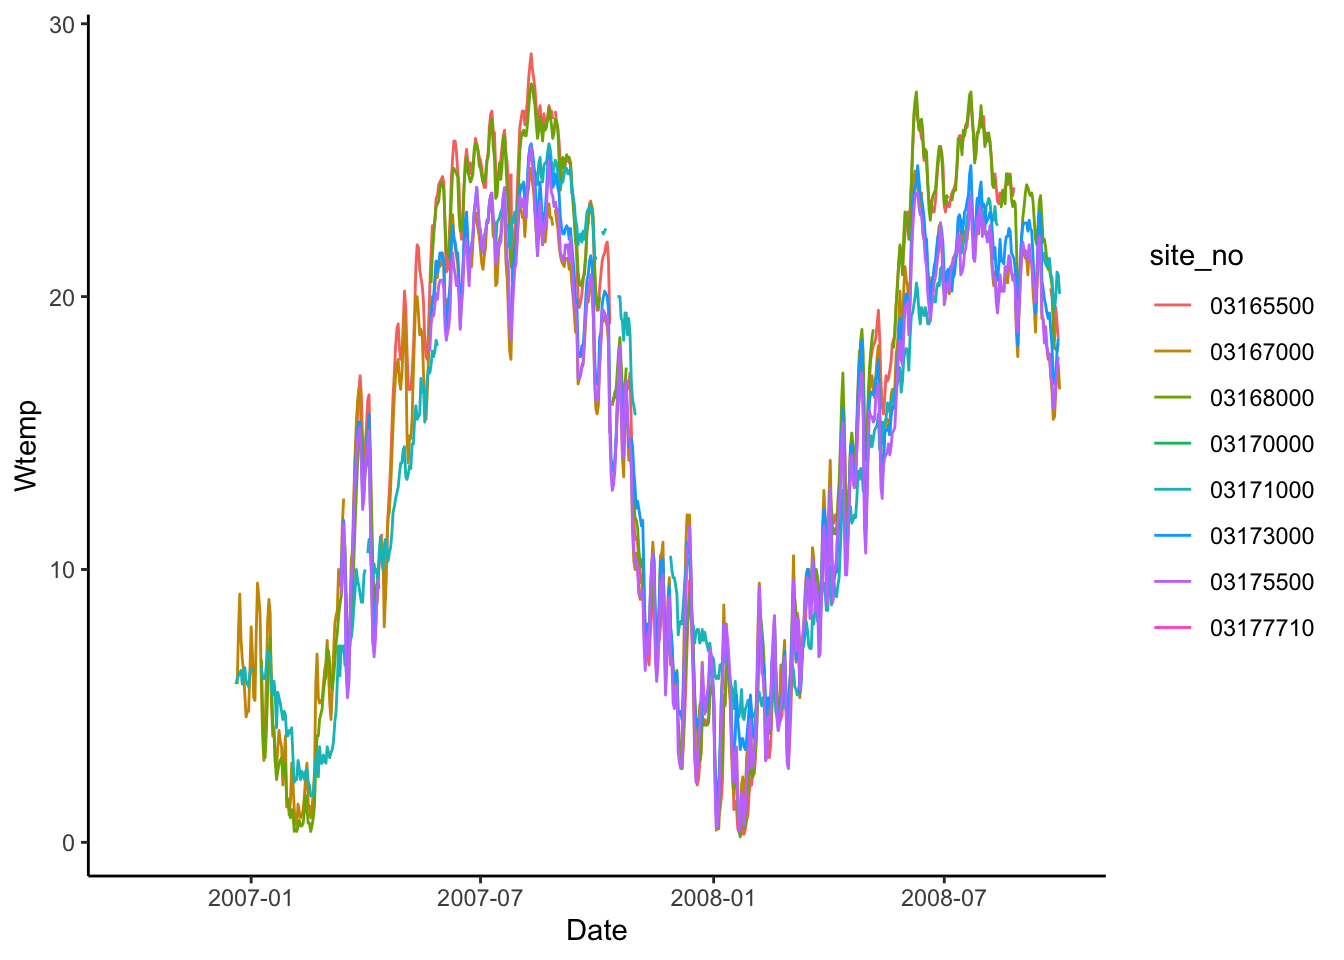
\includegraphics{Hydroinformatics_Bookdown_files/figure-latex/unnamed-chunk-62-1.pdf}

We can add site names with\ldots.More joins! Our swva\_sites data has the names of the sites in human-friendly language. The column in the downloaded data and in the swva\_sites data is called ``site\_no'' so we just give that to the ``by'' argument. Perform a left join to add the names of the sites to the data.

Then use select to remove some of the unnecessary columns.

Then make the plot and then snazz it up with labels and a non-junky theme.

\begin{Shaded}
\begin{Highlighting}[]
\NormalTok{swva\_dat\_clean }\OtherTok{\textless{}{-}} \FunctionTok{left\_join}\NormalTok{(swva\_dat, swva\_sites, }\AttributeTok{by =} \StringTok{"site\_no"}\NormalTok{) }\SpecialCharTok{\%\textgreater{}\%}
  \FunctionTok{select}\NormalTok{(station\_nm, site\_no, Date, Flow, Wtemp, dec\_lat\_va, dec\_long\_va)}

\NormalTok{swva\_dat\_clean }\SpecialCharTok{\%\textgreater{}\%} \FunctionTok{ggplot}\NormalTok{(}\FunctionTok{aes}\NormalTok{(}\AttributeTok{x =}\NormalTok{ Date, }\AttributeTok{y =}\NormalTok{ Wtemp, }\AttributeTok{color =}\NormalTok{ station\_nm)) }\SpecialCharTok{+}
  \FunctionTok{geom\_line}\NormalTok{()}\SpecialCharTok{+}
  \FunctionTok{ylab}\NormalTok{(}\StringTok{"Water temperature (deg C)"}\NormalTok{)}\SpecialCharTok{+}
  \FunctionTok{xlab}\NormalTok{(}\FunctionTok{element\_blank}\NormalTok{())}\SpecialCharTok{+}
  \FunctionTok{labs}\NormalTok{(}\AttributeTok{color =} \StringTok{"Gage Site"}\NormalTok{)}\SpecialCharTok{+}
  \FunctionTok{theme\_classic}\NormalTok{()}
\end{Highlighting}
\end{Shaded}

\begin{verbatim}
## Warning: Removed 2218 row(s) containing missing values (geom_path).
\end{verbatim}

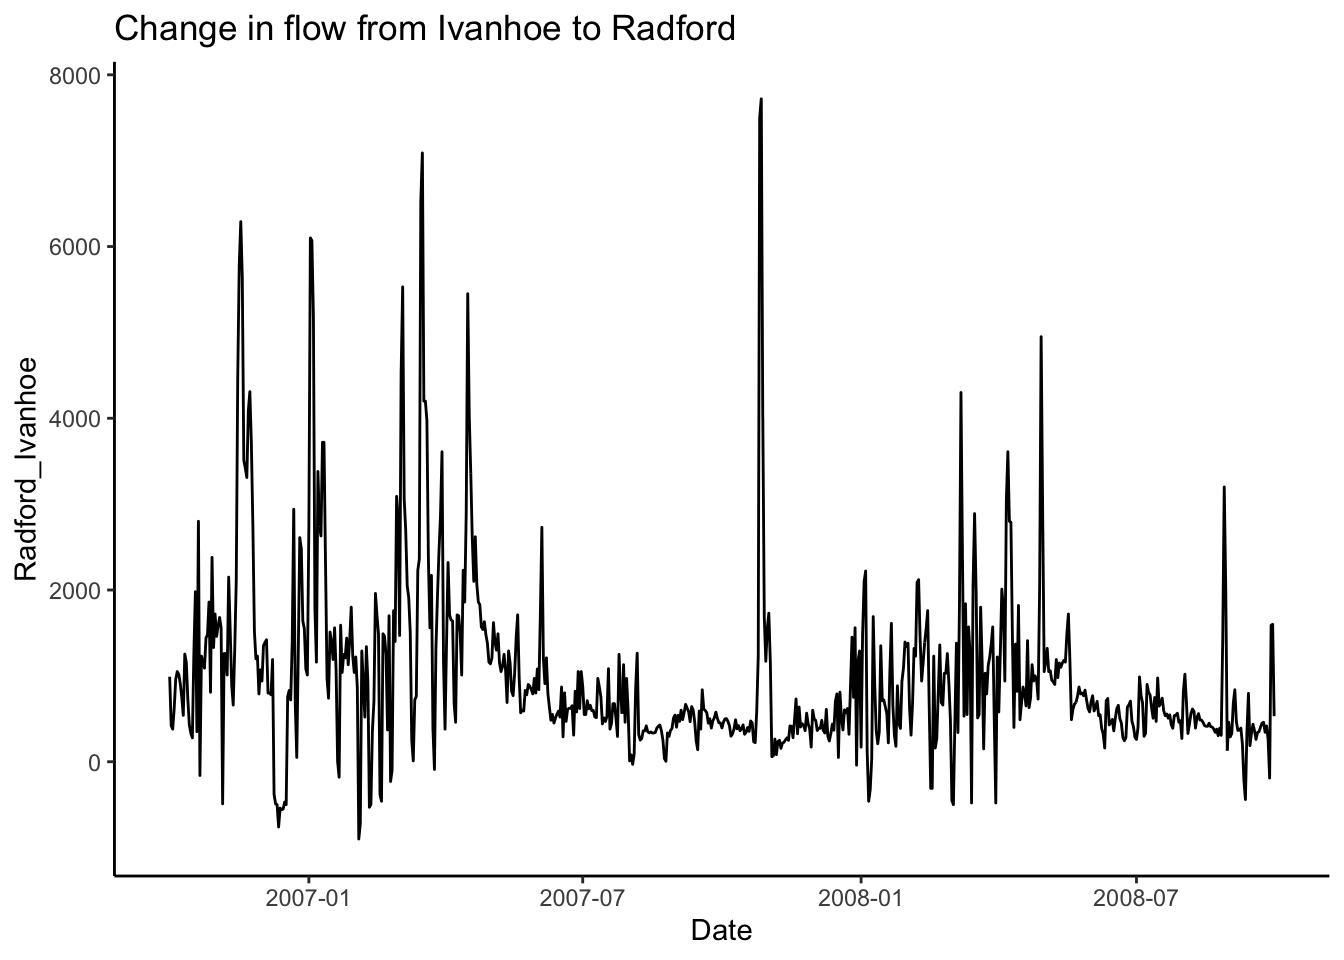
\includegraphics{Hydroinformatics_Bookdown_files/figure-latex/unnamed-chunk-63-1.pdf}

\hypertarget{pivoting-wide-and-long-data}{%
\section{Pivoting: wide and long data}\label{pivoting-wide-and-long-data}}

Okay, so with the data above: what would you do if you wanted to subtract the discharge or temperature of one gage from another on the same river: to compute rate of change between the two sites, for instance.

You could split them into two objects, then join based on date?

Or\ldots now hear me out\ldots{} you could PIVOT them.

A two-dimensional object can be either long or wide. Each has it's advantages.

\textbf{LONG}

Each observation has it's own row. In the first image below, the table on the left is long because each measure of ``cases'' has it's own row. It's year and country are identified by a second column, and the values in that column repeat a lot. (Look at country and year in the table on the left)

\textbf{WIDE}

Observations of different things have their own columns. In the second image below, notice in the right hand table there is a ``cases'' and ``population'' column rather than an identifier in a separate column like in the table on the left.

\textbf{Why?}

Long and wide data are more efficient for different things. Think about plotting a data set with 10 stream gages. If they are in a long format, you can just add color = Gage to your ggplot aes(). If they are in a wide format, meaning each gage has it's own column, you'd have to write a new geom for EACH gage, because they're all in separate columns.

Now imagine you want to do some math to create new data: let's say cases divided by population in the second image below\ldots. How would you even do that using the data on the left? With the wide data on the right it is simply mutate(casesPERpop = cases / population).

Finally, which table is easier to read in TABLE format (not a plot) in each of the two images below? Wide data is much more fitting for tables.

\begin{figure}
\centering
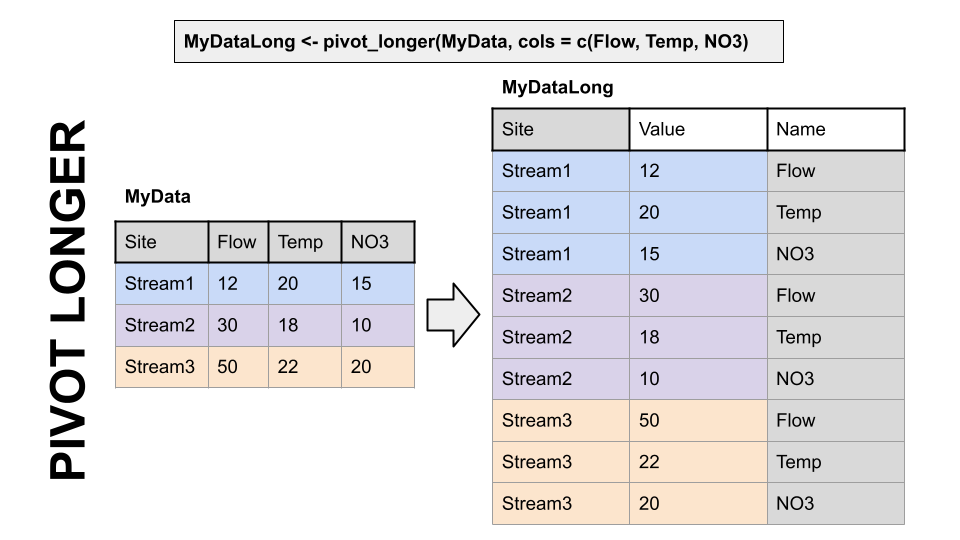
\includegraphics{images/pivot_longer.png}
\caption{Pivoting to a longer format}
\end{figure}

\begin{figure}
\centering
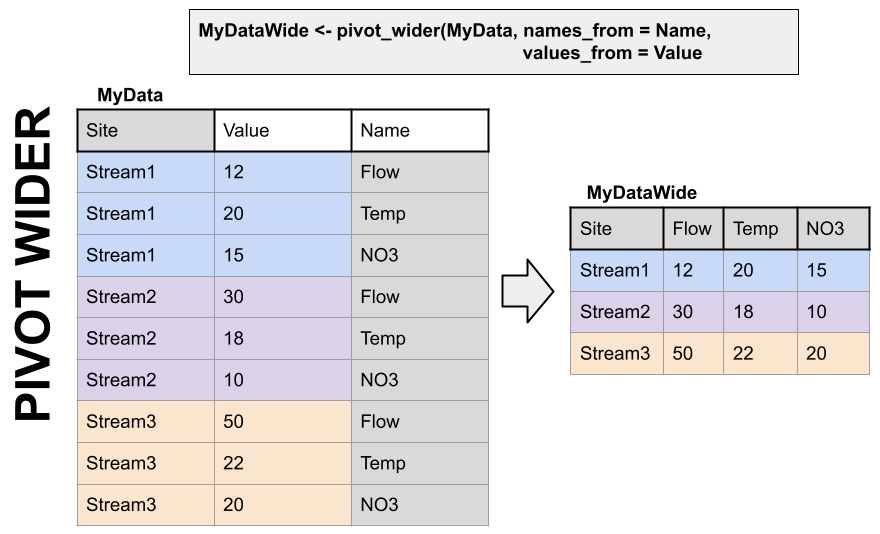
\includegraphics{images/pivot_wider.png}
\caption{Pivoting to a wider format}
\end{figure}

dplyr, part of the tidyverse, has functions to convert data between wide and long data. I have to look up the syntax every single time I use them. But they are VERY useful.

\hypertarget{pivot-examples}{%
\section{Pivot Examples}\label{pivot-examples}}

Back to our original question: I want to subtract the flow at Ivanhoe from the flow at Radford on the new river to see how much flow increases between the two sites through time.

To do this I am going to use pivot\_wider() to give Ivanhoe and Radford discharges their own column.

First, we will use select to trim the data to just what we need, then call pivot\_wider telling it which data to use for the new column names (names\_from = station\_nm) and what values we want to pivot into the data under those columns (values\_from = Flow).

Then, subtract the two and make a plot!

\begin{Shaded}
\begin{Highlighting}[]
\CommentTok{\#Pivot so we can compute diffs between one river and others}

\NormalTok{swva\_wide }\OtherTok{\textless{}{-}}\NormalTok{ swva\_dat\_clean }\SpecialCharTok{\%\textgreater{}\%} \FunctionTok{select}\NormalTok{(station\_nm, Flow, Date) }\SpecialCharTok{\%\textgreater{}\%}
  \FunctionTok{pivot\_wider}\NormalTok{(}\AttributeTok{names\_from =}\NormalTok{ station\_nm, }\AttributeTok{values\_from =}\NormalTok{ Flow)}

\NormalTok{swva\_wide }\OtherTok{\textless{}{-}}\NormalTok{ swva\_wide }\SpecialCharTok{\%\textgreater{}\%} \FunctionTok{mutate}\NormalTok{(}\AttributeTok{Radford\_Ivanhoe =} \StringTok{\textasciigrave{}}\AttributeTok{NEW RIVER AT RADFORD, VA}\StringTok{\textasciigrave{}} \SpecialCharTok{{-}} \StringTok{\textasciigrave{}}\AttributeTok{NEW RIVER AT IVANHOE, VA}\StringTok{\textasciigrave{}}\NormalTok{)}

\FunctionTok{ggplot}\NormalTok{(swva\_wide, }\FunctionTok{aes}\NormalTok{(}\AttributeTok{x =}\NormalTok{ Date, }\AttributeTok{y =}\NormalTok{ Radford\_Ivanhoe))}\SpecialCharTok{+}
  \FunctionTok{geom\_line}\NormalTok{()}\SpecialCharTok{+}
  \FunctionTok{ggtitle}\NormalTok{(}\StringTok{"Change in flow from Ivanhoe to Radford"}\NormalTok{)}\SpecialCharTok{+}
  \FunctionTok{theme\_classic}\NormalTok{()}
\end{Highlighting}
\end{Shaded}

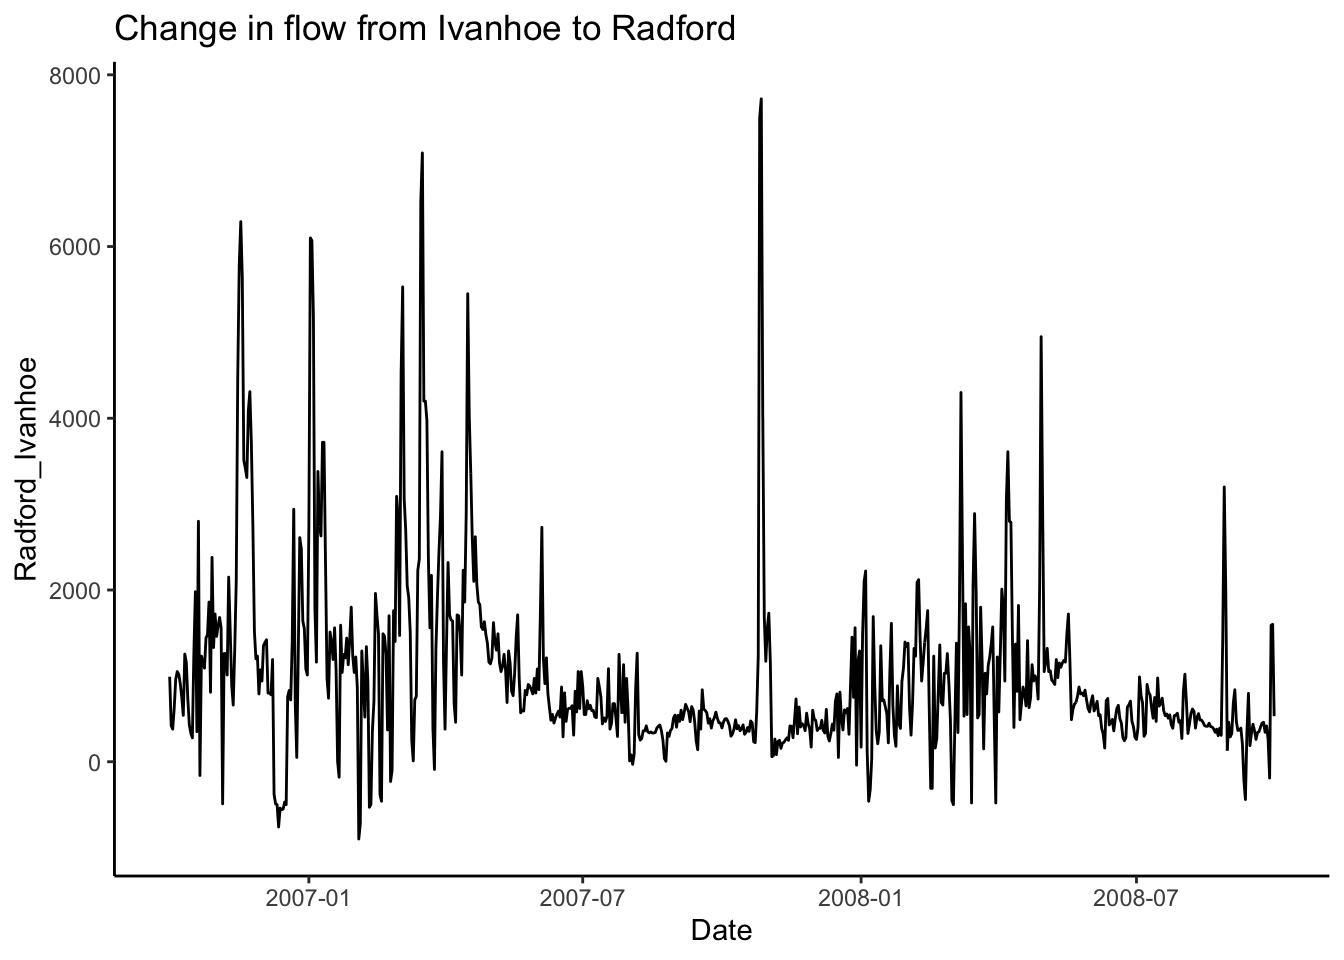
\includegraphics{Hydroinformatics_Bookdown_files/figure-latex/unnamed-chunk-64-1.pdf}

To further illustrate how to move between long and wide data and when to use them, let's grab some water quality data. This process will also review some of the other concepts from this topic.

In the chunk below we will look to see what sites have data for nitrate and chloride in our swva bounding box from above. We will them filter them to just stream sites (leave out groundwater and springs). And finally we will download the nitrate and chloride data for those sites.

\begin{Shaded}
\begin{Highlighting}[]
\CommentTok{\#Nitrate as nitrate and chloride}
\NormalTok{params }\OtherTok{\textless{}{-}} \FunctionTok{c}\NormalTok{(}\StringTok{"00940"}\NormalTok{, }\StringTok{"71851"}\NormalTok{)}

\CommentTok{\#what sites in our bounding box have cloride and nitrate}
\NormalTok{swva\_chem\_sites }\OtherTok{\textless{}{-}} \FunctionTok{whatNWISsites}\NormalTok{(}\AttributeTok{bBox =}\NormalTok{ swva, }
                            \AttributeTok{parameterCd =}\NormalTok{ params)}

\CommentTok{\#filte to just stream water}
\NormalTok{swva\_chem\_sites }\OtherTok{\textless{}{-}} \FunctionTok{filter}\NormalTok{(swva\_chem\_sites, site\_tp\_cd }\SpecialCharTok{==} \StringTok{"ST"}\NormalTok{)}

\NormalTok{wqdat }\OtherTok{\textless{}{-}} \FunctionTok{readNWISqw}\NormalTok{(}\AttributeTok{siteNumber =}\NormalTok{ swva\_chem\_sites}\SpecialCharTok{$}\NormalTok{site\_no, }
                    \AttributeTok{parameterCd =}\NormalTok{ params)}

\FunctionTok{comment}\NormalTok{(wqdat)}
\end{Highlighting}
\end{Shaded}

\begin{verbatim}
## NULL
\end{verbatim}

Now, let's clean things up a bit.

Join the parameter names from parameterCdFile and then join the site names from swva\_chem\_site. Then select just the columns we want, and finally filter the remaining data to just look at sites from the New River.

To illustrate the functionality of the data in this format, plot Chloride for each site, and then plot Chloride AND Nitrate, using the parameter name in facet\_wrap.

\begin{Shaded}
\begin{Highlighting}[]
\NormalTok{wqdat\_clean }\OtherTok{\textless{}{-}}\NormalTok{ wqdat }\SpecialCharTok{\%\textgreater{}\%} 
  \FunctionTok{left\_join}\NormalTok{(parameterCdFile, }\AttributeTok{by =} \FunctionTok{c}\NormalTok{(}\StringTok{"parm\_cd"} \OtherTok{=} \StringTok{"parameter\_cd"}\NormalTok{)) }\SpecialCharTok{\%\textgreater{}\%}
  \FunctionTok{left\_join}\NormalTok{(swva\_chem\_sites, }\AttributeTok{by =} \StringTok{"site\_no"}\NormalTok{) }\SpecialCharTok{\%\textgreater{}\%}
  \FunctionTok{select}\NormalTok{(station\_nm, sample\_dt, sample\_tm, result\_va, srsname, parameter\_units) }\SpecialCharTok{\%\textgreater{}\%}
  \FunctionTok{filter}\NormalTok{(}\FunctionTok{str\_detect}\NormalTok{(station\_nm, }\StringTok{"NEW RIVER"}\NormalTok{))}
  
\NormalTok{wqdat\_clean }\SpecialCharTok{\%\textgreater{}\%} \FunctionTok{filter}\NormalTok{(srsname }\SpecialCharTok{==} \StringTok{"Chloride"}\NormalTok{) }\SpecialCharTok{\%\textgreater{}\%}
  \FunctionTok{ggplot}\NormalTok{(}\FunctionTok{aes}\NormalTok{(}\AttributeTok{x =}\NormalTok{ sample\_dt, }\AttributeTok{y =}\NormalTok{ result\_va, }\AttributeTok{color =}\NormalTok{ station\_nm)) }\SpecialCharTok{+}
  \FunctionTok{geom\_point}\NormalTok{()}\SpecialCharTok{+}
  \FunctionTok{ylab}\NormalTok{(}\StringTok{"Chloride (mg/L)"}\NormalTok{)}\SpecialCharTok{+}
  \FunctionTok{xlab}\NormalTok{(}\FunctionTok{element\_blank}\NormalTok{())}\SpecialCharTok{+}
  \FunctionTok{labs}\NormalTok{(}\AttributeTok{color =} \StringTok{"Site"}\NormalTok{)}\SpecialCharTok{+}
  \FunctionTok{theme\_classic}\NormalTok{()}
\end{Highlighting}
\end{Shaded}

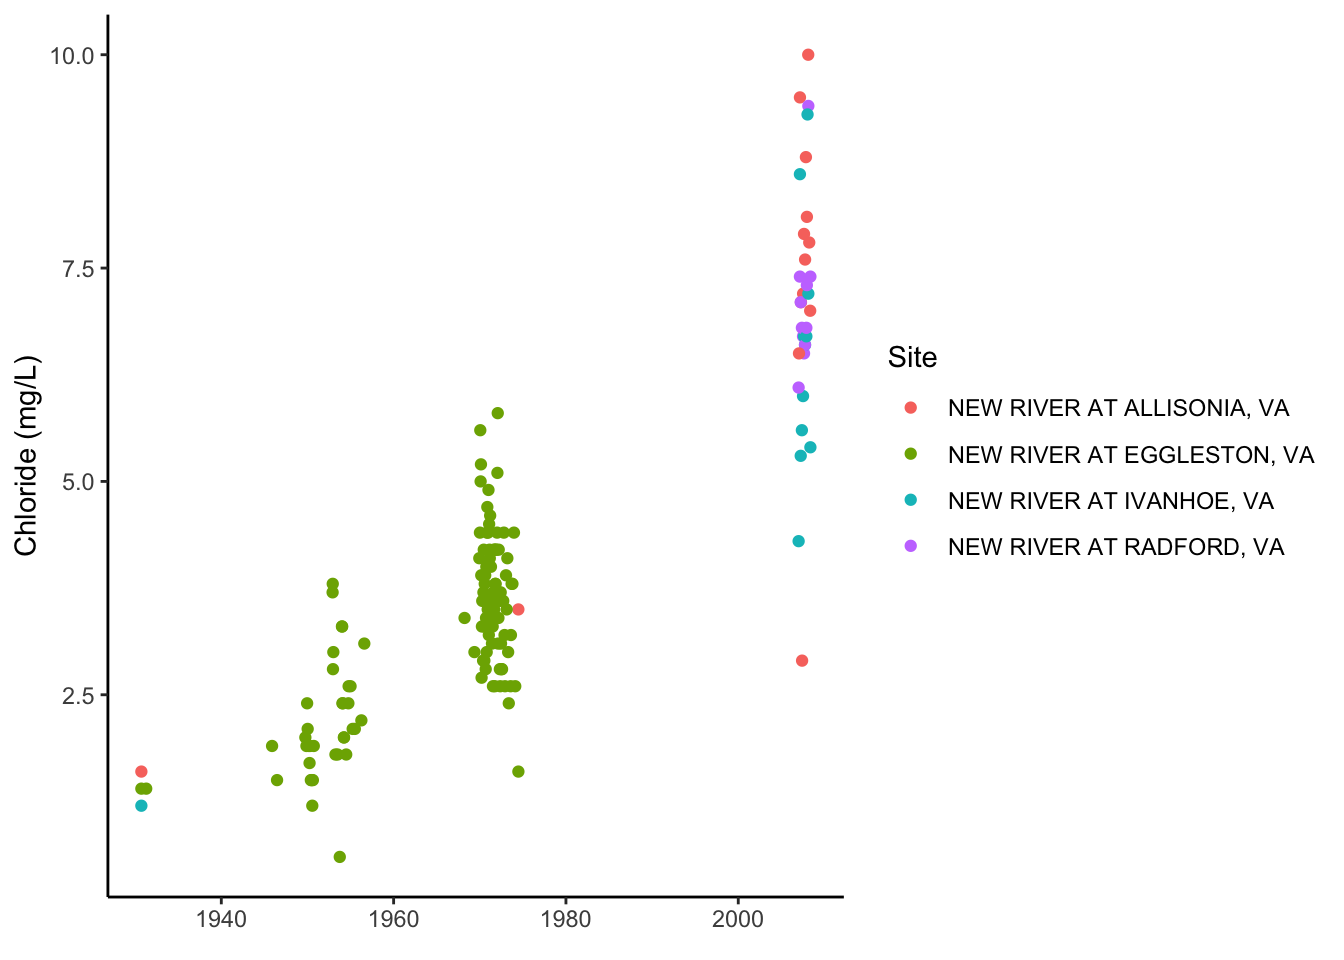
\includegraphics{Hydroinformatics_Bookdown_files/figure-latex/unnamed-chunk-66-1.pdf}

\begin{Shaded}
\begin{Highlighting}[]
\NormalTok{wqdat\_clean }\SpecialCharTok{\%\textgreater{}\%}
  \FunctionTok{ggplot}\NormalTok{(}\FunctionTok{aes}\NormalTok{(}\AttributeTok{x =}\NormalTok{ sample\_dt, }\AttributeTok{y =}\NormalTok{ result\_va, }\AttributeTok{color =}\NormalTok{ station\_nm)) }\SpecialCharTok{+}
  \FunctionTok{geom\_point}\NormalTok{()}\SpecialCharTok{+}
  \FunctionTok{facet\_wrap}\NormalTok{(}\AttributeTok{facets =} \StringTok{"srsname"}\NormalTok{, }\AttributeTok{nrow =} \DecValTok{2}\NormalTok{)}\SpecialCharTok{+}
  \FunctionTok{ylab}\NormalTok{(}\StringTok{"Concentration (mg/L)"}\NormalTok{)}\SpecialCharTok{+}
  \FunctionTok{xlab}\NormalTok{(}\FunctionTok{element\_blank}\NormalTok{())}\SpecialCharTok{+}
  \FunctionTok{labs}\NormalTok{(}\AttributeTok{color =} \StringTok{"Site"}\NormalTok{)}\SpecialCharTok{+}
  \FunctionTok{theme\_classic}\NormalTok{()}
\end{Highlighting}
\end{Shaded}

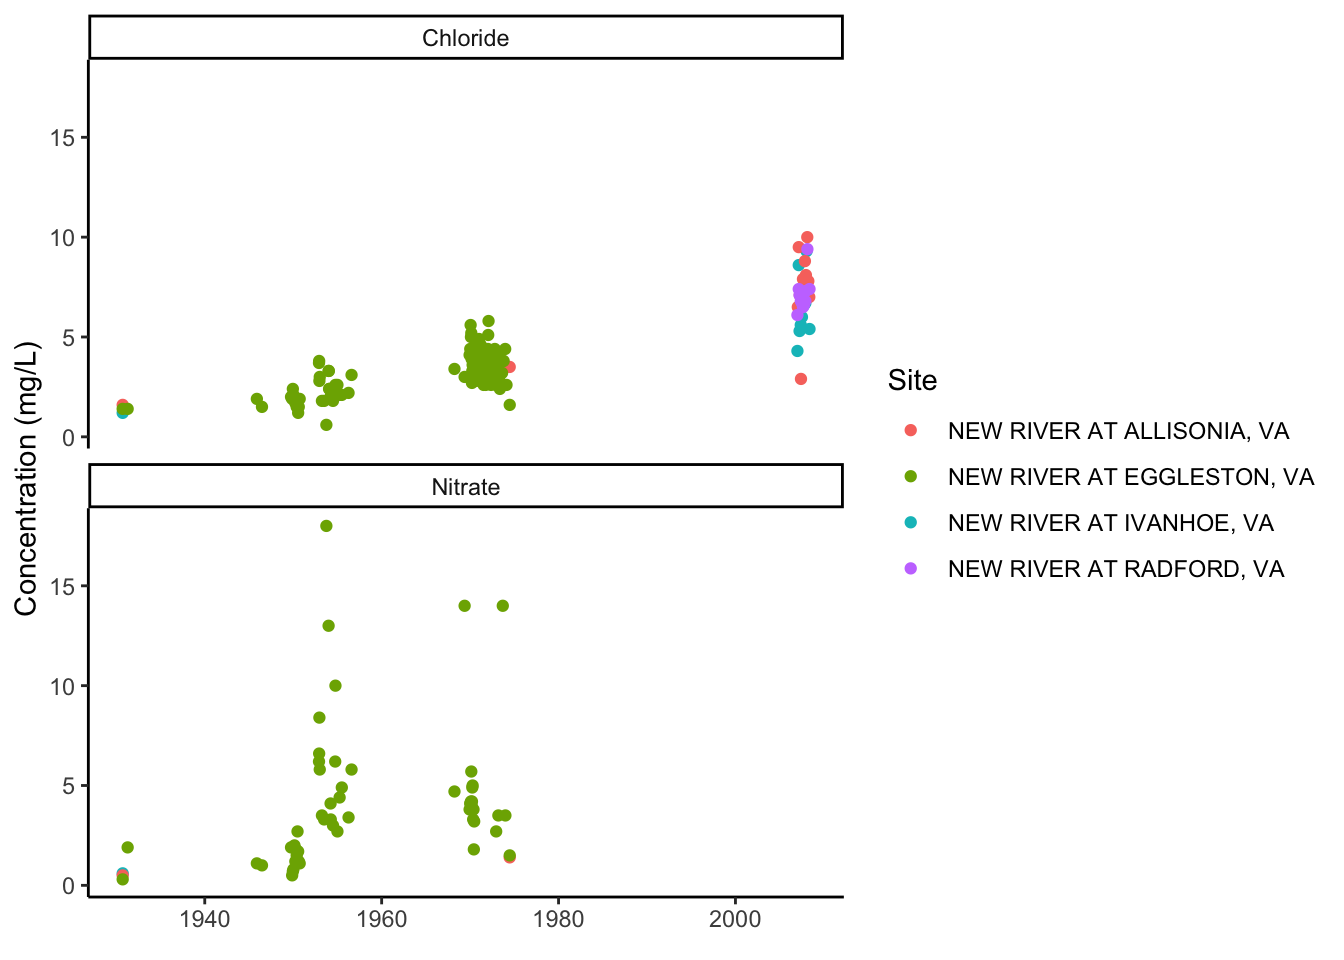
\includegraphics{Hydroinformatics_Bookdown_files/figure-latex/unnamed-chunk-66-2.pdf}

Now let's say we want to calculate something with chloride and nitrate. We need to make the data wide so we have a nitrate column and a chloride column. Do that below. What goes into values\_from? what goes into names\_from?

Next, plot Chloride + Nitrate. Could you do this with the data in the previous format?

Finally, use pivot\_longer to transform the data back into a long format. Often you'll get data in a wide format and need to convert it to long, and we haven't tried that yet. The only argument you'll need to pass to pivot\_longer() in this case is to tell it what columns to turn into the new DATA column (using the cols = ) parameter.

\begin{Shaded}
\begin{Highlighting}[]
\CommentTok{\#make wqdat\_clean wide}

\NormalTok{wqdat\_wide }\OtherTok{\textless{}{-}}\NormalTok{ wqdat\_clean }\SpecialCharTok{\%\textgreater{}\%} \FunctionTok{select}\NormalTok{(}\SpecialCharTok{{-}}\NormalTok{parameter\_units) }\SpecialCharTok{\%\textgreater{}\%}
  \FunctionTok{pivot\_wider}\NormalTok{(}\AttributeTok{values\_from =}\NormalTok{ result\_va, }\AttributeTok{names\_from =}\NormalTok{ srsname)}

\FunctionTok{ggplot}\NormalTok{(wqdat\_wide, }\FunctionTok{aes}\NormalTok{(}\AttributeTok{x =}\NormalTok{ sample\_dt, }\AttributeTok{y =}\NormalTok{ Chloride }\SpecialCharTok{+}\NormalTok{ Nitrate)) }\SpecialCharTok{+}
  \FunctionTok{geom\_point}\NormalTok{()}
\end{Highlighting}
\end{Shaded}

\begin{verbatim}
## Warning: Removed 106 rows containing missing values (geom_point).
\end{verbatim}

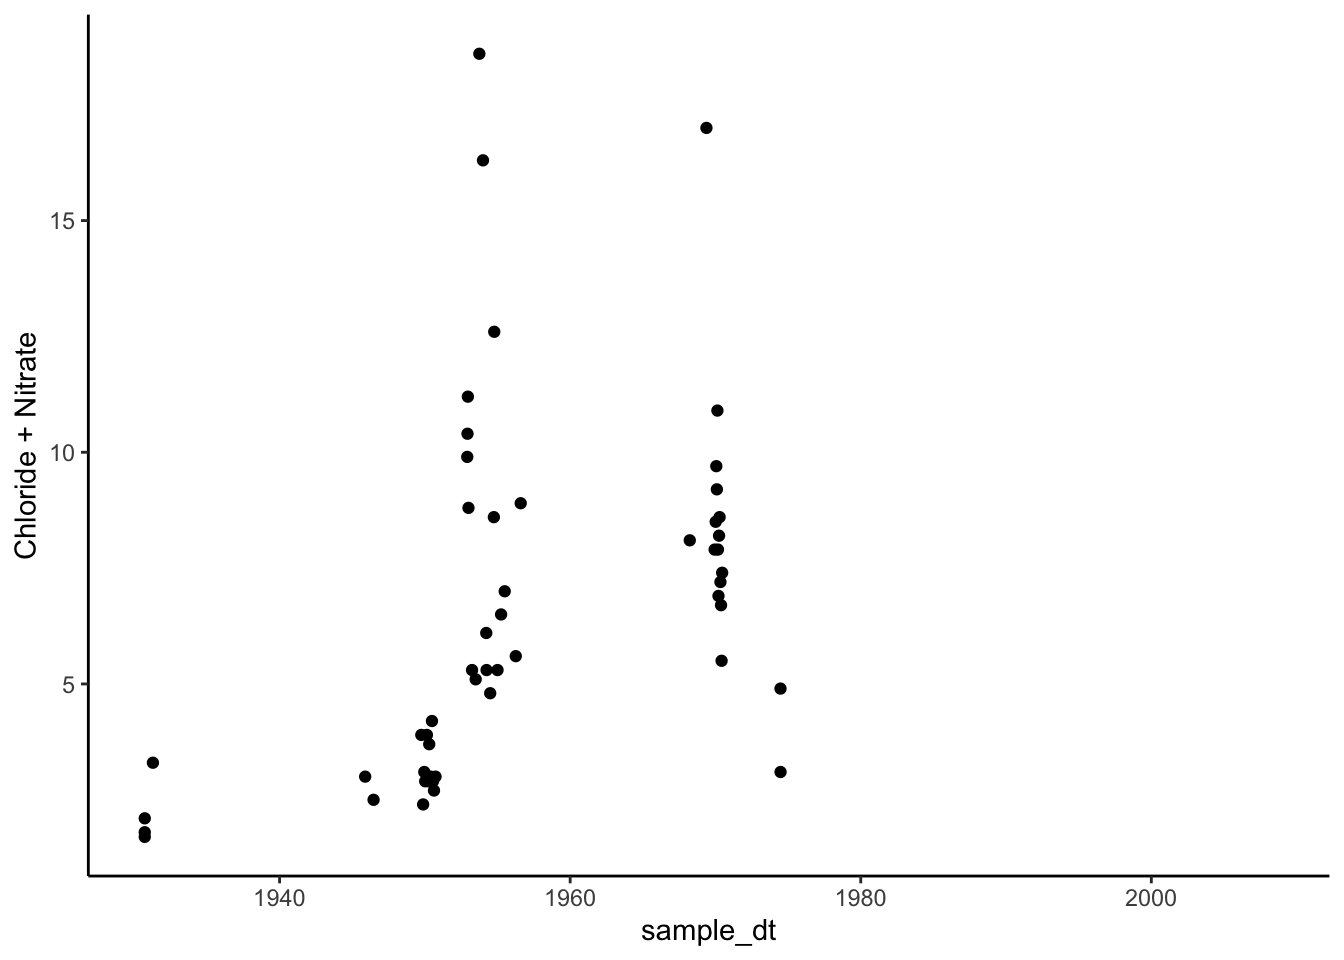
\includegraphics{Hydroinformatics_Bookdown_files/figure-latex/unnamed-chunk-67-1.pdf}

\begin{Shaded}
\begin{Highlighting}[]
\NormalTok{wqlonger }\OtherTok{\textless{}{-}}\NormalTok{ wqdat\_wide }\SpecialCharTok{\%\textgreater{}\%}
  \FunctionTok{pivot\_longer}\NormalTok{(}\AttributeTok{cols =} \FunctionTok{c}\NormalTok{(}\StringTok{"Chloride"}\NormalTok{, }\StringTok{"Nitrate"}\NormalTok{))}
\end{Highlighting}
\end{Shaded}

\hypertarget{joinpivotDR}{%
\chapter{ACTIVITY Joins Pivots dataRetrieval}\label{joinpivotDR}}

Get this document at the template repository on github: \url{https://github.com/VT-Hydroinformatics/7-Activity-Joins-Pivots_dataRetrieval}

\hypertarget{load-the-tidyverse-dataretrieval-and-patchwork-packages.}{%
\section{Load the tidyverse, dataRetrieval, and patchwork packages.}\label{load-the-tidyverse-dataretrieval-and-patchwork-packages.}}

\begin{Shaded}
\begin{Highlighting}[]
\FunctionTok{library}\NormalTok{(tidyverse)}
\FunctionTok{library}\NormalTok{(dataRetrieval)}
\FunctionTok{library}\NormalTok{(patchwork)}
\end{Highlighting}
\end{Shaded}

\hypertarget{problem-1-2}{%
\section{Problem 1}\label{problem-1-2}}

Using readNWISqw(), read all the chloride (00940) data for the New River at Radford (03171000). Use the head() function to print the beginning of the output from readNWISqw.

\hypertarget{problem-2-2}{%
\section{Problem 2}\label{problem-2-2}}

Using the readNWISdv (daily values) function, download discharge (00060), temperature (00003), and specific conductivity (00095) for the New River at Radford from 2007 to 2009 (regular year). Use renameNWIScolumns() to rename the output of the download. Use head() to show the beginning of the results of your download.

\hypertarget{problem-3-2}{%
\section{Problem 3}\label{problem-3-2}}

Do a left join on newphys and newriver to add the chloride data to the daily discharge, temp, and conductivity data. hint: you will join on the date. Preview your data below the chunk using head().

\hypertarget{problem-4-2}{%
\section{Problem 4}\label{problem-4-2}}

Create a line plot of Date (x) and Flow (y). Create a scatter plot of Date (x) and chloride concentration (y). Put the graphs on top of each other using the patchwork library.

\hypertarget{problem-5-2}{%
\section{Problem 5}\label{problem-5-2}}

Create a scatter plot of Specific Conductivity (y) and Chloride (x). Challenge: what could you do to get rid of the warning this plot generates about NAs.

\hypertarget{problem-6-2}{%
\section{Problem 6}\label{problem-6-2}}

Read in the GG chem subset data and plot Mg\_E1 (x) vs Ca\_E1 (y) as points.

\hypertarget{problem-7}{%
\section{Problem 7}\label{problem-7}}

We want to look at concentrations of each element in the \#6 dataset along the stream (Distance), which is difficult in the current format. Pivot the data into a long format, the data from Ca, Mg, and Na \_E1 columns should be pivoted. Make line plots of each element where y is the concentration and x is distance. Use facet\_wrap() to create a separate plot for each element and use the ``scales'' argument of facet\_wrap to allow each plot to have different y limits.

\hypertarget{Summative1}{%
\chapter{ACTIVITY Summative 1}\label{Summative1}}

Get this document at the template repository on github: \url{https://github.com/VT-Hydroinformatics/8-Test_1}

\hypertarget{instructions}{%
\subsection{Instructions}\label{instructions}}

Please read carefully!\\

Write your code in the provided code chunks and answer any questions by typing outside the chunk.

Comment your code to let me know what you are trying to do, in case something doesn't work.

Turn in a knitted rmd (html or pdf). If you can't get your document to knit when you go to turn it in, just comment out the lines of code that are causing the knit to fail, knit the document, and submit.

\hypertarget{problem-1-3}{%
\section{Problem 1}\label{problem-1-3}}

Load the tidyverse, lubridate, and dataRetrieval packages.

\hypertarget{problem-2-3}{%
\section{Problem 2}\label{problem-2-3}}

Read in the McDonald Hollow dataset in the project folder.

What are the data types of the first three columns?

How long is the data (number of rows)?

What is the name of the last column?

\hypertarget{problem-3-3}{%
\section{Problem 3}\label{problem-3-3}}

Plot the stage of the stream (Stage\_m\_pt) on the y axis as a line and the date on the x. These stage data are in meters, convert them to centimeters for the plot.

For all plots in this test, label axes properly and use a theme other than the default.

\hypertarget{problem-4-3}{%
\section{Problem 4}\label{problem-4-3}}

We want to look at the big event that happens from November 11, 2020 to November 27, 2020. Filter the dataset down to this time frame and save it separately. Make a plot with the same setup as in \#3 with these newly saved data.

\hypertarget{problem-5-3}{%
\section{Problem 5}\label{problem-5-3}}

For this storm, we are curious about how conductivity changes with the stream level. To do this, make a scatter plot that shows Stage on the x axis and specific conductivity (SpC\_mScm) on the y. (units: mScm) Color the points on the plot using the datetime column. Use the plot to describe how specific conductivity changes with stream stage throughout the storm. (not functionally, just how the values change)

\hypertarget{problem-6-3}{%
\section{Problem 6}\label{problem-6-3}}

Continuing to look at the storm, as an exploratory data analysis, we want to create a plot that shows all the parameters measured. To do this, pivot the STORM EVENT data so there is a column that has the values for all the parameters measured as individual rows, along with another column that identifies the type of measurement. Then use facet\_wrap with the ``name'' column (or whatever you call it) as the facet. Be sure to set the parameters of facet\_wrap such that the y axes are all allowed to be different ranges.

EX:\\
Date Value Name\\
10/1/20 12 Stage\\
10/1/20 6 Temp\\
\ldots.

\hypertarget{problem-7-1}{%
\section{Problem 7}\label{problem-7-1}}

We want to create a table that clearly shows the differences in water temperature for the three months at the two locations (flow and pool) in the FULL data set (not the storm subset). To do this: Create a new column in the full dataset called ``month'' and set it equal to the month of the datetime column using the month() function. Then group your dataset by month and summarize temperature at each location by mean. Save these results to a new object and output it so it appears below your chunk when you knit. Be sure the object has descriptive column names.

You can do this all in one statement using pipes.

\hypertarget{problem-8}{%
\section{Problem 8}\label{problem-8}}

Plot the distribution of the flow temperature and show as vertical lines on the plot the mean, median, and IQR. Be careful about how you show IQR. Look at the definition and then think about how you would put it on the plot. Describe in the text above the chunk what color is what statistic in the plot. Using the shape of the distribution and the measures you plotted, explain why you think the distribution is normal or not. What statistical test could you perform to see if it is normal?

\hypertarget{problem-9}{%
\section{Problem 9}\label{problem-9}}

In this question we will get and format data for three USGS gages.

Gages: 03177710, 03173000, 03177480\\
Discharge in cubic feet per second (cfs) code: 00060

\begin{enumerate}
\def\labelenumi{\alph{enumi}.}
\item
  Read and save the gage information for the three gages using readNWISsite().
\item
  Use the readNWISdv() function to read and save the daily discharge values for the following three gages for the 2020 water year (10-01-2019 to 9-30-2020). And then use the renameNWIScolumns() function to make the names human-friendly.
\item
  Join the gage site information from (a) to the data from (b) so you can reference the gages by their names.
\end{enumerate}

\hypertarget{problem-10}{%
\section{Problem 10}\label{problem-10}}

Using the data from \#9, Plot flow on the y axis and date on the x axis, showing the data as a line, and coloring by gage name.

\hypertarget{fdcs}{%
\chapter{Flow Duration Curves}\label{fdcs}}

Get this document and a version with empty code chunks at the template repository on github: \url{https://github.com/VT-Hydroinformatics/9-Flow-Duration-Curves}

Alright team. So far we have learned to wrangle data, make plots, and look at data distributions. Now it is time to put all that knowledge to use.

We are on our way to doing analyses of extreme discharge events: low flow statistics and floods. But in order to do that, we need to understand a common way to look at data distributions in hydrology: the flow duration curve. As you'll see below, this is basically just a different way of looking at a pdf, and it can take some getting used to. But it is also a very useful tool!

As always let's load the packages we will use: tidyverse, dataRetrieval, lubridate, and patchwork. Patchwork will help us make a multi-panel graph in the last part of the exercise.

We will also use theme\_set() in this chunk so we don't have to change the ggplot theme every time we make a plot.

\begin{Shaded}
\begin{Highlighting}[]
\FunctionTok{library}\NormalTok{(tidyverse)}
\FunctionTok{library}\NormalTok{(dataRetrieval)}
\FunctionTok{library}\NormalTok{(lubridate)}
\FunctionTok{library}\NormalTok{(patchwork)}

\CommentTok{\#set plot theme for the document so we }
\CommentTok{\#don\textquotesingle{}t have to do it in every plot}
\FunctionTok{theme\_set}\NormalTok{(}\FunctionTok{theme\_classic}\NormalTok{())}
\end{Highlighting}
\end{Shaded}

\hypertarget{get-data}{%
\section{Get data}\label{get-data}}

To start, let's grab the USGS discharge data for the gage in Linville NC from 1960 to 2020.

We will download the data using USGS dataRetrieval and look at a line plot.

\begin{Shaded}
\begin{Highlighting}[]
\NormalTok{siteno }\OtherTok{\textless{}{-}} \StringTok{"02138500"} \CommentTok{\#Linville NC}
\NormalTok{startDate }\OtherTok{\textless{}{-}} \StringTok{"1960{-}01{-}01"}
\NormalTok{endDate }\OtherTok{\textless{}{-}} \StringTok{"2020{-}01{-}01"}
\NormalTok{parameter }\OtherTok{\textless{}{-}} \StringTok{"00060"}

\NormalTok{Qdat }\OtherTok{\textless{}{-}} \FunctionTok{readNWISdv}\NormalTok{(siteno, parameter, startDate, endDate) }\SpecialCharTok{\%\textgreater{}\%} 
  \FunctionTok{renameNWISColumns}\NormalTok{()}

\CommentTok{\#Look at the data}
\NormalTok{Qdat }\SpecialCharTok{\%\textgreater{}\%} \FunctionTok{ggplot}\NormalTok{(}\FunctionTok{aes}\NormalTok{(}\AttributeTok{x =}\NormalTok{ Date, }\AttributeTok{y =}\NormalTok{ Flow))}\SpecialCharTok{+}
  \FunctionTok{geom\_line}\NormalTok{()}
\end{Highlighting}
\end{Shaded}

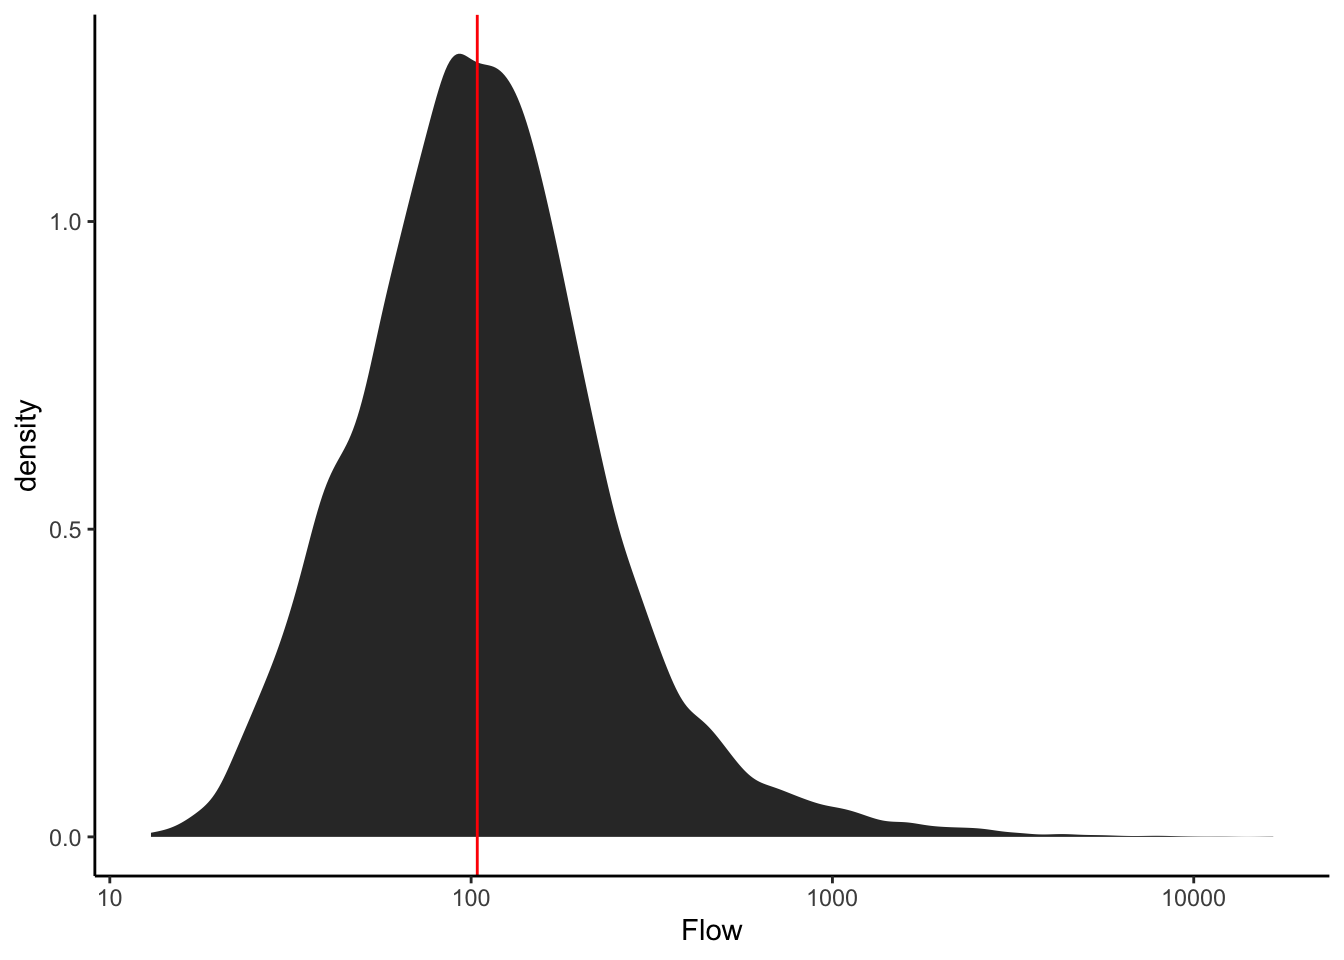
\includegraphics{Hydroinformatics_Bookdown_files/figure-latex/unnamed-chunk-87-1.pdf}

\hypertarget{review-describe-the-distribution}{%
\section{Review: describe the distribution}\label{review-describe-the-distribution}}

Make a plot to view the distribution of the discharge data.

\begin{itemize}
\tightlist
\item
  What is the median flow value?
\item
  What does this tell us about flow at that river?
\item
  How often is the river at or below that value?
\item
  Could you pick that number off the plot?
\item
  What about the flow the river is at or above only 5\% of the time?
\end{itemize}

\begin{Shaded}
\begin{Highlighting}[]
\NormalTok{Qdat }\SpecialCharTok{\%\textgreater{}\%} \FunctionTok{ggplot}\NormalTok{(}\FunctionTok{aes}\NormalTok{(Flow))}\SpecialCharTok{+}
  \FunctionTok{stat\_density}\NormalTok{()}\SpecialCharTok{+}
  \FunctionTok{scale\_x\_log10}\NormalTok{()}\SpecialCharTok{+}
  \FunctionTok{geom\_vline}\NormalTok{(}\AttributeTok{xintercept =} \FunctionTok{median}\NormalTok{(Qdat}\SpecialCharTok{$}\NormalTok{Flow), }\AttributeTok{color =} \StringTok{"red"}\NormalTok{)}
\end{Highlighting}
\end{Shaded}

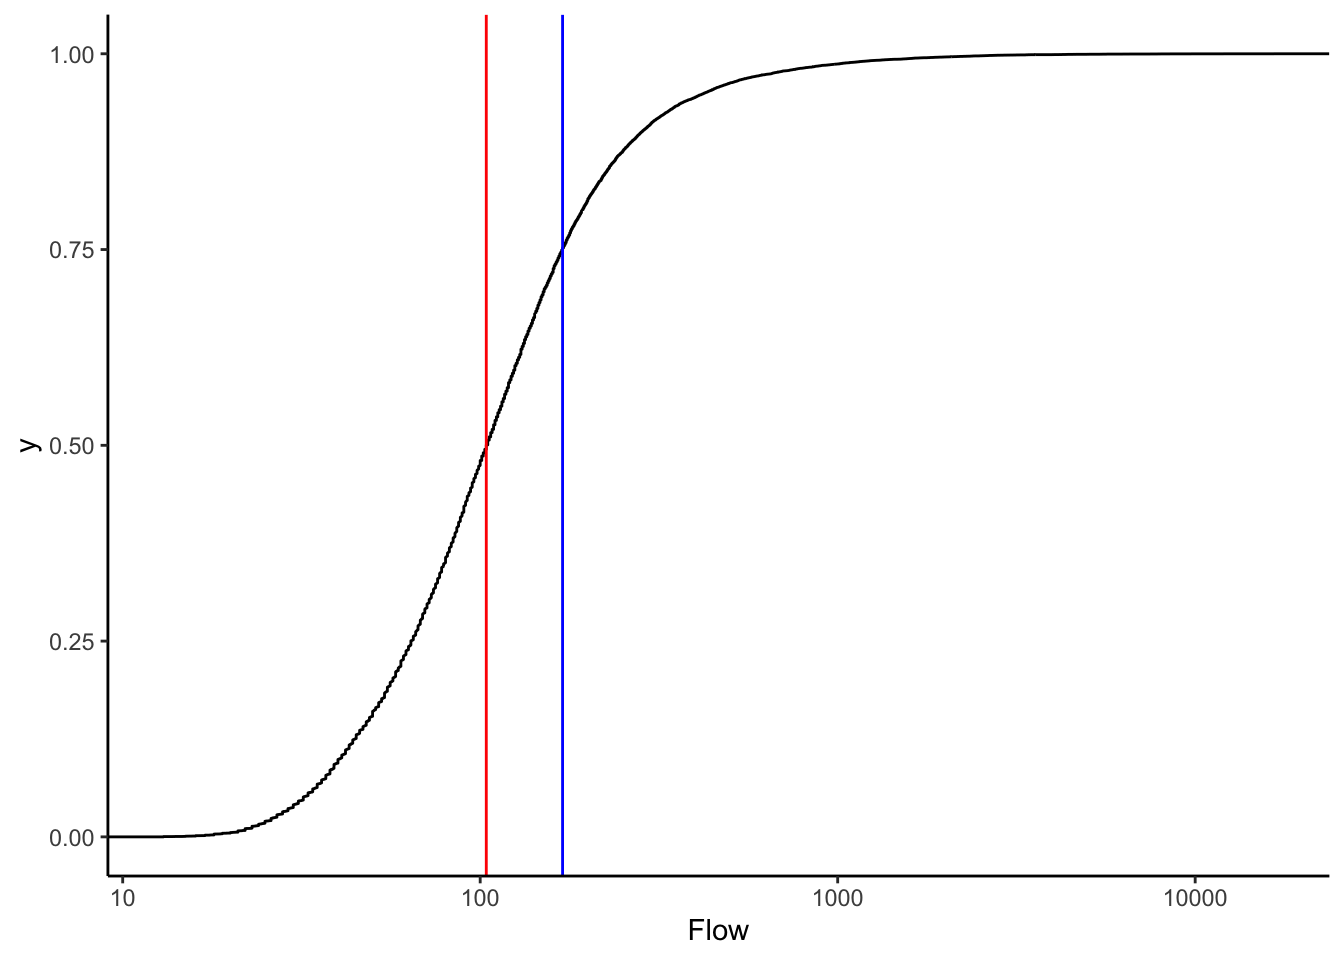
\includegraphics{Hydroinformatics_Bookdown_files/figure-latex/unnamed-chunk-88-1.pdf}

\hypertarget{ecdfs}{%
\section{ECDFs}\label{ecdfs}}

Let's look at an Empirical Cumulative Density Function (ECDF) of the data.

Look at this carefully, what does it show? How is it different from the pdf of the data?

Plot the median again. Without the line on the plot, how would you tell where the median is?

Given your answer to the question above, can you determine the flow the river is at or above only 25\% of the time? Think carefully about what the y axis of the ECDF means.

\begin{Shaded}
\begin{Highlighting}[]
\NormalTok{Qdat }\SpecialCharTok{\%\textgreater{}\%} \FunctionTok{ggplot}\NormalTok{(}\FunctionTok{aes}\NormalTok{(Flow))}\SpecialCharTok{+}
  \FunctionTok{stat\_ecdf}\NormalTok{()}\SpecialCharTok{+}
  \FunctionTok{scale\_x\_log10}\NormalTok{()}\SpecialCharTok{+}
  \FunctionTok{geom\_vline}\NormalTok{(}\AttributeTok{xintercept =} \FunctionTok{median}\NormalTok{(Qdat}\SpecialCharTok{$}\NormalTok{Flow), }\AttributeTok{color =} \StringTok{"red"}\NormalTok{)}\SpecialCharTok{+}
  \FunctionTok{geom\_vline}\NormalTok{(}\AttributeTok{xintercept =} \FunctionTok{quantile}\NormalTok{(Qdat}\SpecialCharTok{$}\NormalTok{Flow)[}\DecValTok{4}\NormalTok{], }\AttributeTok{color =} \StringTok{"blue"}\NormalTok{)}
\end{Highlighting}
\end{Shaded}

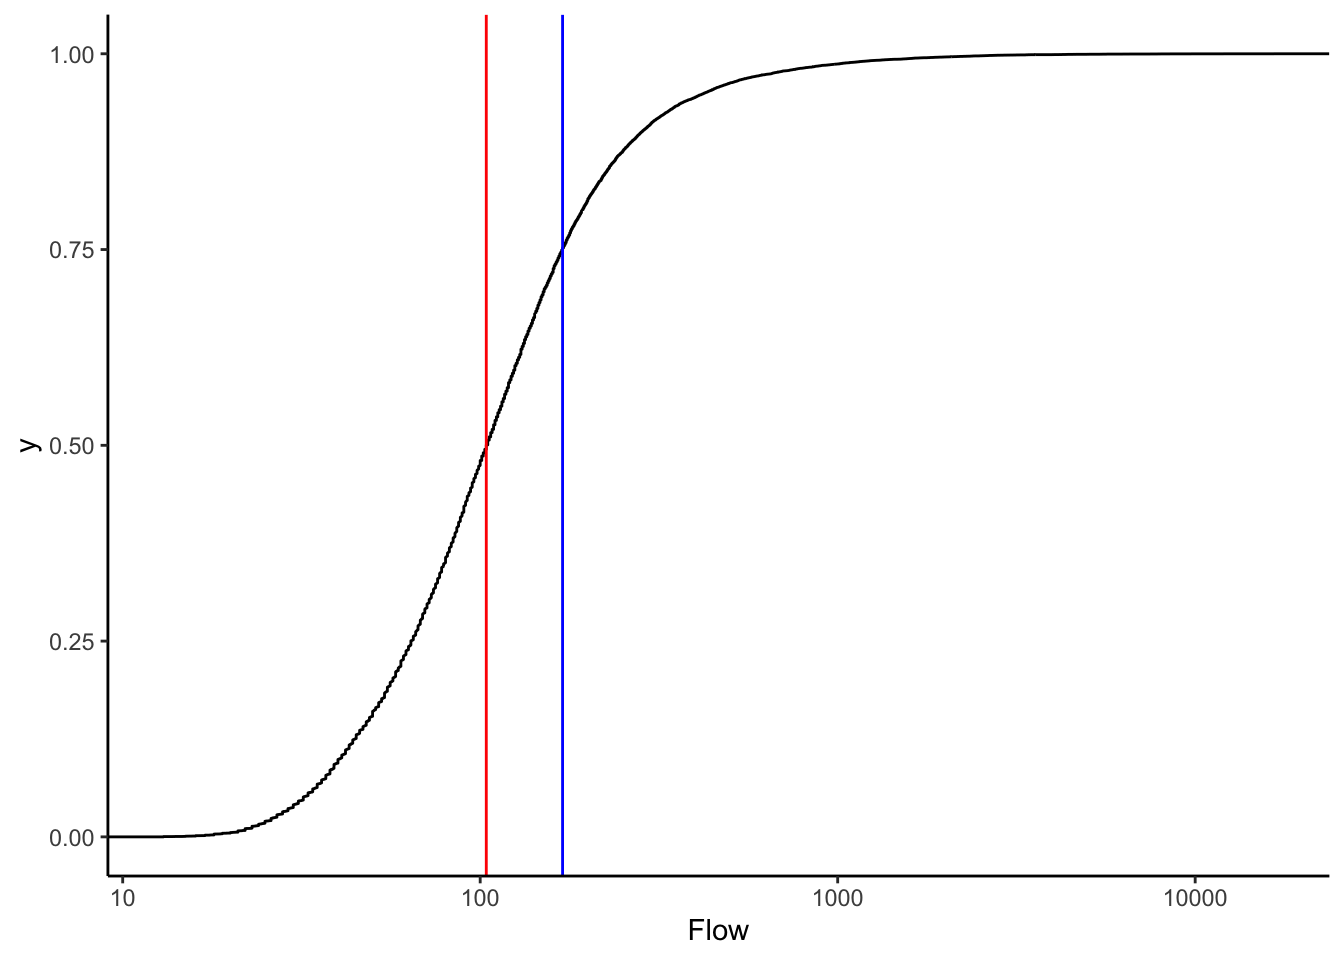
\includegraphics{Hydroinformatics_Bookdown_files/figure-latex/unnamed-chunk-89-1.pdf}

\hypertarget{calculate-flow-exceedence-probabilities}{%
\section{Calculate flow exceedence probabilities}\label{calculate-flow-exceedence-probabilities}}

In hydrology, it is common to look at a similar representation of flow distributions, but with flow on the Y axis and ``\% time flow is equaled or exceeded'' on the X axis. There are a number of ways we could make this plot: for example we could transform the axes of the plot above or we could use the function that results from the ECDF function in R to calculate exceedence probabilities at flow throughout our range of flows. But for our purposes, we are just going to calculate it manually.

We are going to calculate our own exceedence probabilities because knowing how to do this will hopefully help us understand what a flow duration curve is AND we will need to do similar things in our high and low flow analyses.

The formula for exceedence probability (P) is below. What do we need to calculate this?

Exceedence probability (P), Probability a flow is equaled or exceeded

\(P = 100 * [M / (n + 1)]\)

M = Ranked position of the flow
n = total number of observations in data record

Here's a description of what we will do:

\begin{quote}
Pass our Qdat data to mutate and create a new column that is equal to the ranks of the discharge column.
\end{quote}

\begin{quote}
Then pass that result to mutate again and create another column equal exceedence probability (P) * 100, which will give us \%.
\end{quote}

\begin{Shaded}
\begin{Highlighting}[]
\CommentTok{\#Flow is negative in rank() to make }
\CommentTok{\#high flows ranked low (\#1)}
\NormalTok{Qdat }\OtherTok{\textless{}{-}}\NormalTok{ Qdat }\SpecialCharTok{\%\textgreater{}\%}
  \FunctionTok{mutate}\NormalTok{(}\AttributeTok{rank =} \FunctionTok{rank}\NormalTok{(}\SpecialCharTok{{-}}\NormalTok{Flow)) }\SpecialCharTok{\%\textgreater{}\%}
  \FunctionTok{mutate}\NormalTok{(}\AttributeTok{P =} \DecValTok{100} \SpecialCharTok{*}\NormalTok{ (rank }\SpecialCharTok{/}\NormalTok{ (}\FunctionTok{length}\NormalTok{(Flow) }\SpecialCharTok{+} \DecValTok{1}\NormalTok{)))}
\end{Highlighting}
\end{Shaded}

\hypertarget{plot-a-flow-duration-curve-using-the-probabilities}{%
\section{Plot a Flow Duration Curve using the probabilities}\label{plot-a-flow-duration-curve-using-the-probabilities}}

Now construct the following plot: A line with P on the x axis and flow on the y axis. Name the x axis ``\% Time flow equaled or exceeded'' and log the y axis.

That's a flow duration curve!

Questions about the flow duration curve:

\begin{itemize}
\tightlist
\item
  How often is a flow of 100 cfs exceeded at this gage?
\item
  Is flow more variable for flows exceeded 0-25\% or of the time or 75-100\% * of the time?
\item
  How can you tell?
\item
  These data are daily observations. Given that, what is a more accurate name for the x axis?
\item
  What would the X axis be called if we were using maximum yearly data?
\end{itemize}

\begin{Shaded}
\begin{Highlighting}[]
\NormalTok{Qdat }\SpecialCharTok{\%\textgreater{}\%} \FunctionTok{ggplot}\NormalTok{(}\FunctionTok{aes}\NormalTok{(}\AttributeTok{x =}\NormalTok{ P, }\AttributeTok{y =}\NormalTok{ Flow))}\SpecialCharTok{+}
  \FunctionTok{geom\_line}\NormalTok{()}\SpecialCharTok{+}
  \FunctionTok{scale\_y\_log10}\NormalTok{()}\SpecialCharTok{+}
  \FunctionTok{xlab}\NormalTok{(}\StringTok{"\% Time flow equalled or exceeded"}\NormalTok{)}\SpecialCharTok{+}
  \FunctionTok{ylab}\NormalTok{(}\StringTok{"Q (cfs)"}\NormalTok{)}
\end{Highlighting}
\end{Shaded}

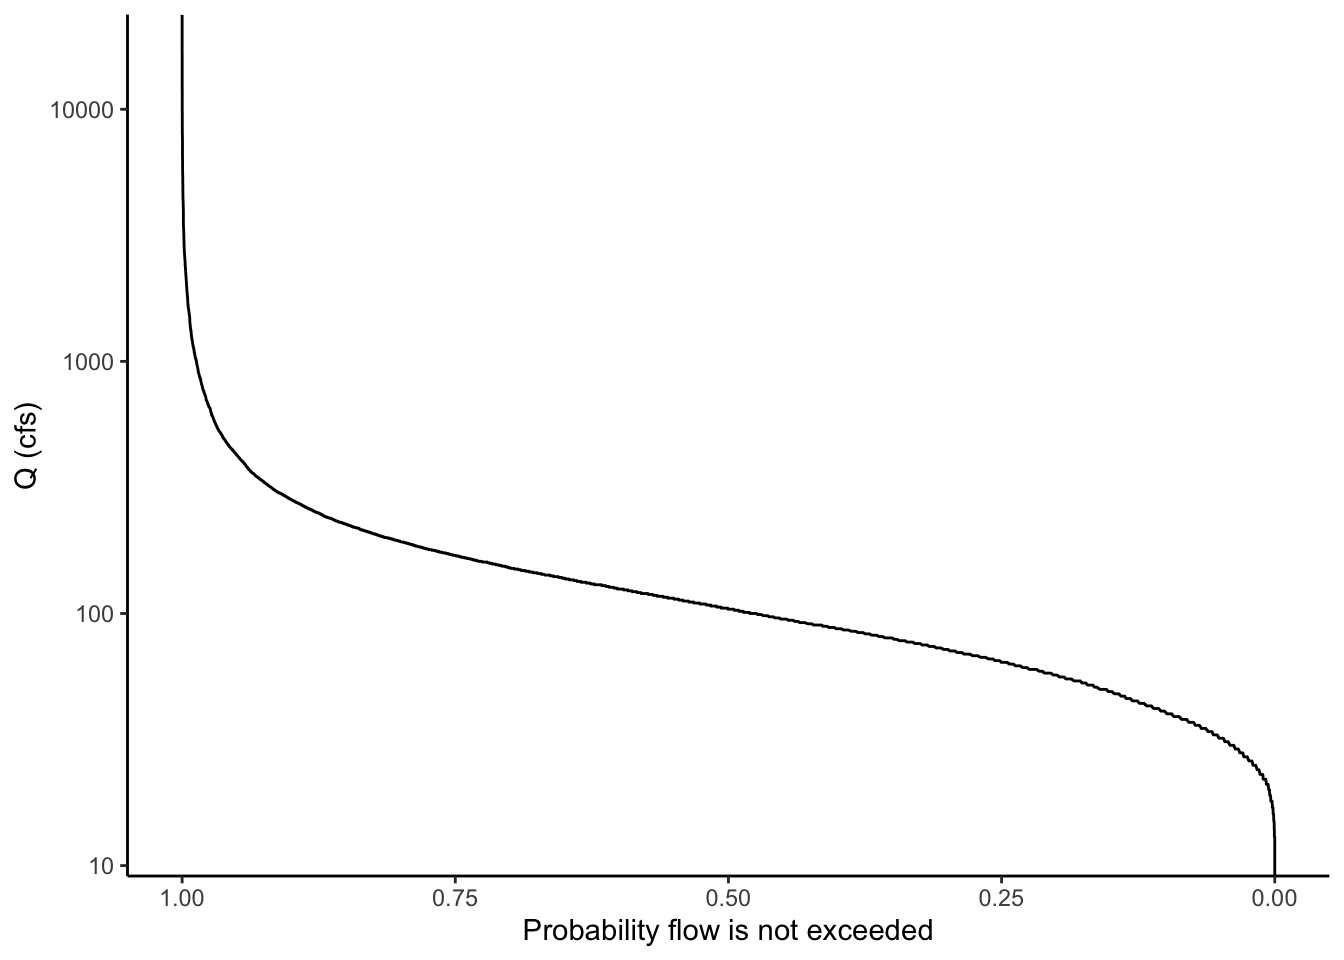
\includegraphics{Hydroinformatics_Bookdown_files/figure-latex/unnamed-chunk-91-1.pdf}

\hypertarget{make-an-almost-fdc-with-stat_ecdf}{%
\section{Make an almost FDC with stat\_ecdf}\label{make-an-almost-fdc-with-stat_ecdf}}

Below is an example of making a very similar plot with the stat\_ecdf() geometry in ggplot. Notice how similar the result is to the one we calculated manually.

To make the plot similar, we will reverse the y axis of the ecdf plot with scale\_y\_reverse and flip the axes (change the x to y and the y to x) with coord\_flip()

\begin{Shaded}
\begin{Highlighting}[]
\NormalTok{Qdat }\SpecialCharTok{\%\textgreater{}\%} \FunctionTok{ggplot}\NormalTok{(}\FunctionTok{aes}\NormalTok{(Flow))}\SpecialCharTok{+}
  \FunctionTok{stat\_ecdf}\NormalTok{()}\SpecialCharTok{+}
  \FunctionTok{scale\_x\_log10}\NormalTok{()}\SpecialCharTok{+}
  \FunctionTok{scale\_y\_reverse}\NormalTok{()}\SpecialCharTok{+}
  \FunctionTok{coord\_flip}\NormalTok{()}\SpecialCharTok{+}
  \FunctionTok{xlab}\NormalTok{(}\StringTok{"Q (cfs)"}\NormalTok{)}\SpecialCharTok{+}
  \FunctionTok{ylab}\NormalTok{(}\StringTok{"Probability flow is not exceeded"}\NormalTok{)}
\end{Highlighting}
\end{Shaded}

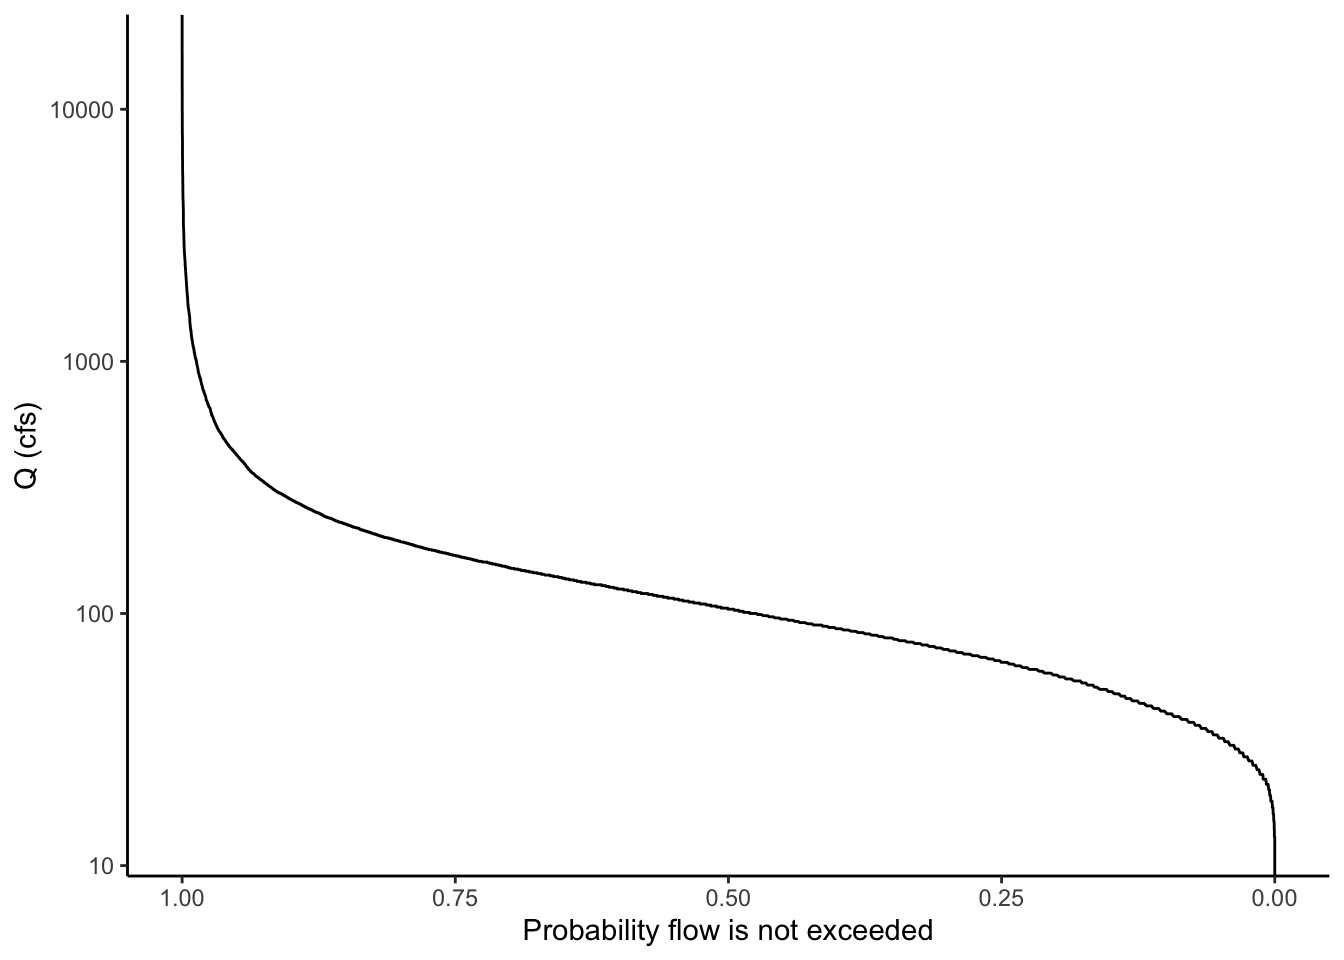
\includegraphics{Hydroinformatics_Bookdown_files/figure-latex/unnamed-chunk-92-1.pdf}

\hypertarget{example-use-of-an-fdc}{%
\section{Example use of an FDC}\label{example-use-of-an-fdc}}

Let's explore one potential use of flow duration curves: examining the differences between two sets of flow data.

From the line plot of the discharge, it looked like the flow regime may have shifted a bit in the data between the early years and newer data. Let's use flow duration curves to examine potential differences. We can come up with groups and then use group\_by to run the analysis by groups instead of the whole dataset.

We are introducing a new function here called case\_when(). This allows you to assign values to a new column based on values in another column. In our case, we are going to name different time periods in our data.

We will then group the data by these periods and calculate exceedence probabilities for each. The procedure works the same, except we add a group\_by statement to group by our time period column before we create the rank and P columns. Then, when we plot, we can just tell ggplot to create different colored lines based on the time period names and it will plot a separate flow duration curve for each. Tidyverse FOR THE WIN!

Describe the differences in flow regime you see between the three periods of 1960-1980, 1980-2000, and 2000-2020.

\begin{Shaded}
\begin{Highlighting}[]
\NormalTok{Qdat }\OtherTok{\textless{}{-}}\NormalTok{ Qdat }\SpecialCharTok{\%\textgreater{}\%}
  \FunctionTok{mutate}\NormalTok{(}\AttributeTok{year =} \FunctionTok{year}\NormalTok{(Date)) }\SpecialCharTok{\%\textgreater{}\%}
  \FunctionTok{mutate}\NormalTok{(}\AttributeTok{period =} \FunctionTok{case\_when}\NormalTok{( year }\SpecialCharTok{\textless{}=} \DecValTok{1980} \SpecialCharTok{\textasciitilde{}} \StringTok{"1960{-}1980"}\NormalTok{,}
\NormalTok{                             year }\SpecialCharTok{\textgreater{}} \DecValTok{1980} \SpecialCharTok{\&}\NormalTok{ year }\SpecialCharTok{\textless{}=} \DecValTok{2000} \SpecialCharTok{\textasciitilde{}} \StringTok{"1980{-}2000"}\NormalTok{,}
\NormalTok{                             year }\SpecialCharTok{\textgreater{}} \DecValTok{2000} \SpecialCharTok{\textasciitilde{}} \StringTok{"2000{-}2020"}\NormalTok{))}

\NormalTok{Qdat }\OtherTok{\textless{}{-}}\NormalTok{ Qdat }\SpecialCharTok{\%\textgreater{}\%}
  \FunctionTok{group\_by}\NormalTok{(period) }\SpecialCharTok{\%\textgreater{}\%}
  \FunctionTok{mutate}\NormalTok{(}\AttributeTok{rank =} \FunctionTok{rank}\NormalTok{(}\SpecialCharTok{{-}}\NormalTok{Flow)) }\SpecialCharTok{\%\textgreater{}\%} 
  \FunctionTok{mutate}\NormalTok{(}\AttributeTok{P =} \DecValTok{100} \SpecialCharTok{*}\NormalTok{ (rank }\SpecialCharTok{/}\NormalTok{ (}\FunctionTok{length}\NormalTok{(Flow) }\SpecialCharTok{+} \DecValTok{1}\NormalTok{)))}

\NormalTok{Qdat }\SpecialCharTok{\%\textgreater{}\%} \FunctionTok{ggplot}\NormalTok{(}\FunctionTok{aes}\NormalTok{(}\AttributeTok{x =}\NormalTok{ P, }\AttributeTok{y =}\NormalTok{ Flow, }\AttributeTok{color =}\NormalTok{ period))}\SpecialCharTok{+}
  \FunctionTok{geom\_line}\NormalTok{()}\SpecialCharTok{+}
  \FunctionTok{scale\_y\_log10}\NormalTok{()}\SpecialCharTok{+}
  \FunctionTok{xlab}\NormalTok{(}\StringTok{"\% Time flow equalled or exceeded"}\NormalTok{)}\SpecialCharTok{+}
  \FunctionTok{ylab}\NormalTok{(}\StringTok{"Q (cfs)"}\NormalTok{)}
\end{Highlighting}
\end{Shaded}

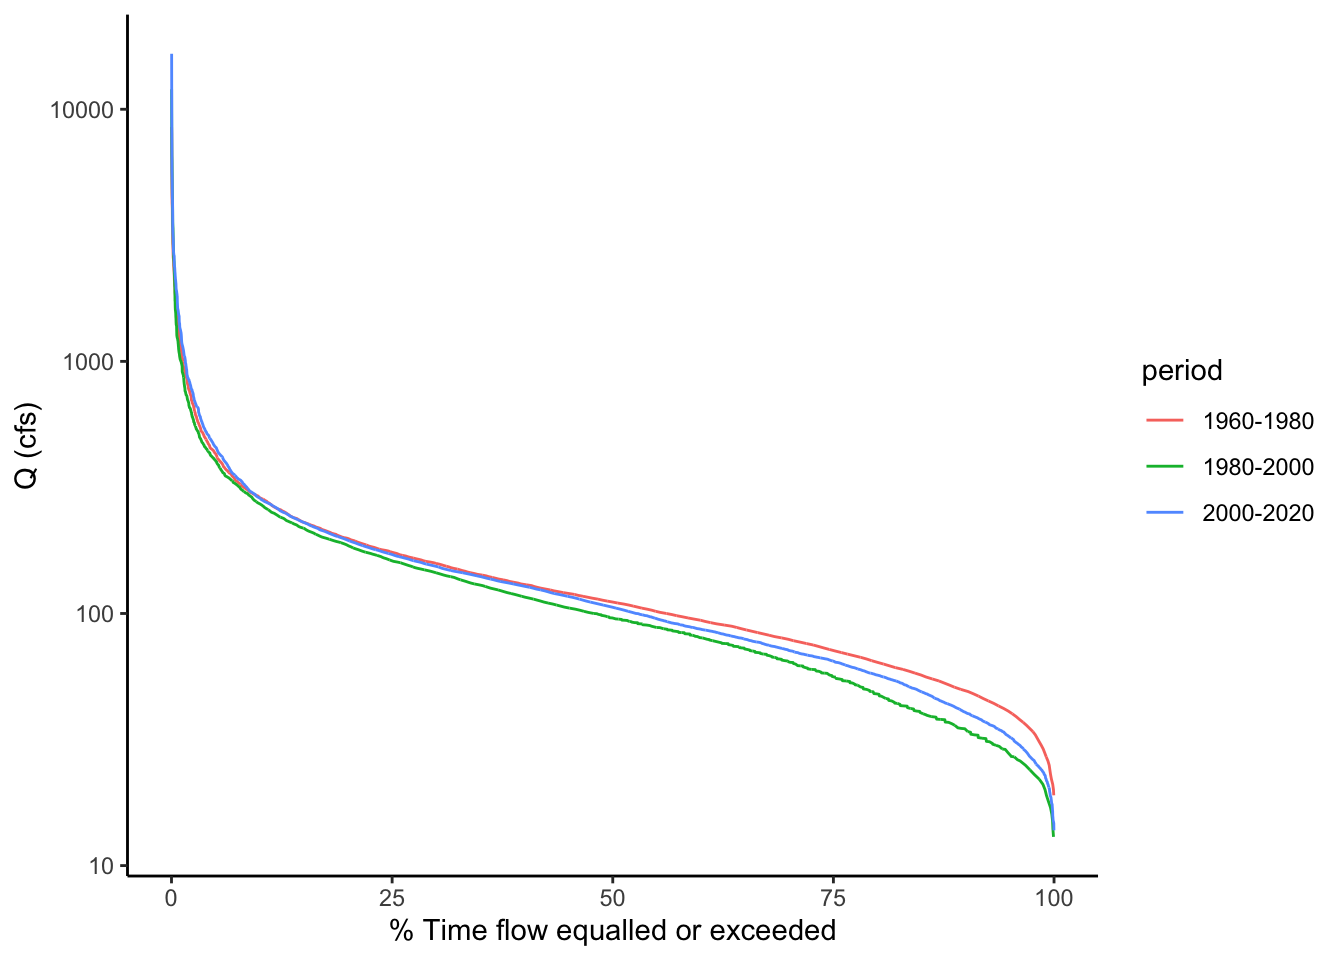
\includegraphics{Hydroinformatics_Bookdown_files/figure-latex/unnamed-chunk-93-1.pdf}

\hypertarget{compare-to-a-boxplot-of-the-same-data}{%
\section{Compare to a boxplot of the same data}\label{compare-to-a-boxplot-of-the-same-data}}

We are really just looking at the data distribution here. Remember another good way to compare distributions is a boxplot. Let's create a boxplot showing flows from these time periods. (we will also mess with the dimensions of the plot so the boxes aren't so wide using fig.width and fig.height in the ``` header above the code chunk)

What are the advantages/disadvantages of the flow duration curves vs.~boxplots?

\begin{Shaded}
\begin{Highlighting}[]
\NormalTok{Qdat }\SpecialCharTok{\%\textgreater{}\%} \FunctionTok{ggplot}\NormalTok{(}\FunctionTok{aes}\NormalTok{(}\AttributeTok{x =}\NormalTok{ period, }\AttributeTok{y =}\NormalTok{ Flow)) }\SpecialCharTok{+}
  \FunctionTok{geom\_boxplot}\NormalTok{()}\SpecialCharTok{+}
  \FunctionTok{scale\_y\_log10}\NormalTok{()}
\end{Highlighting}
\end{Shaded}

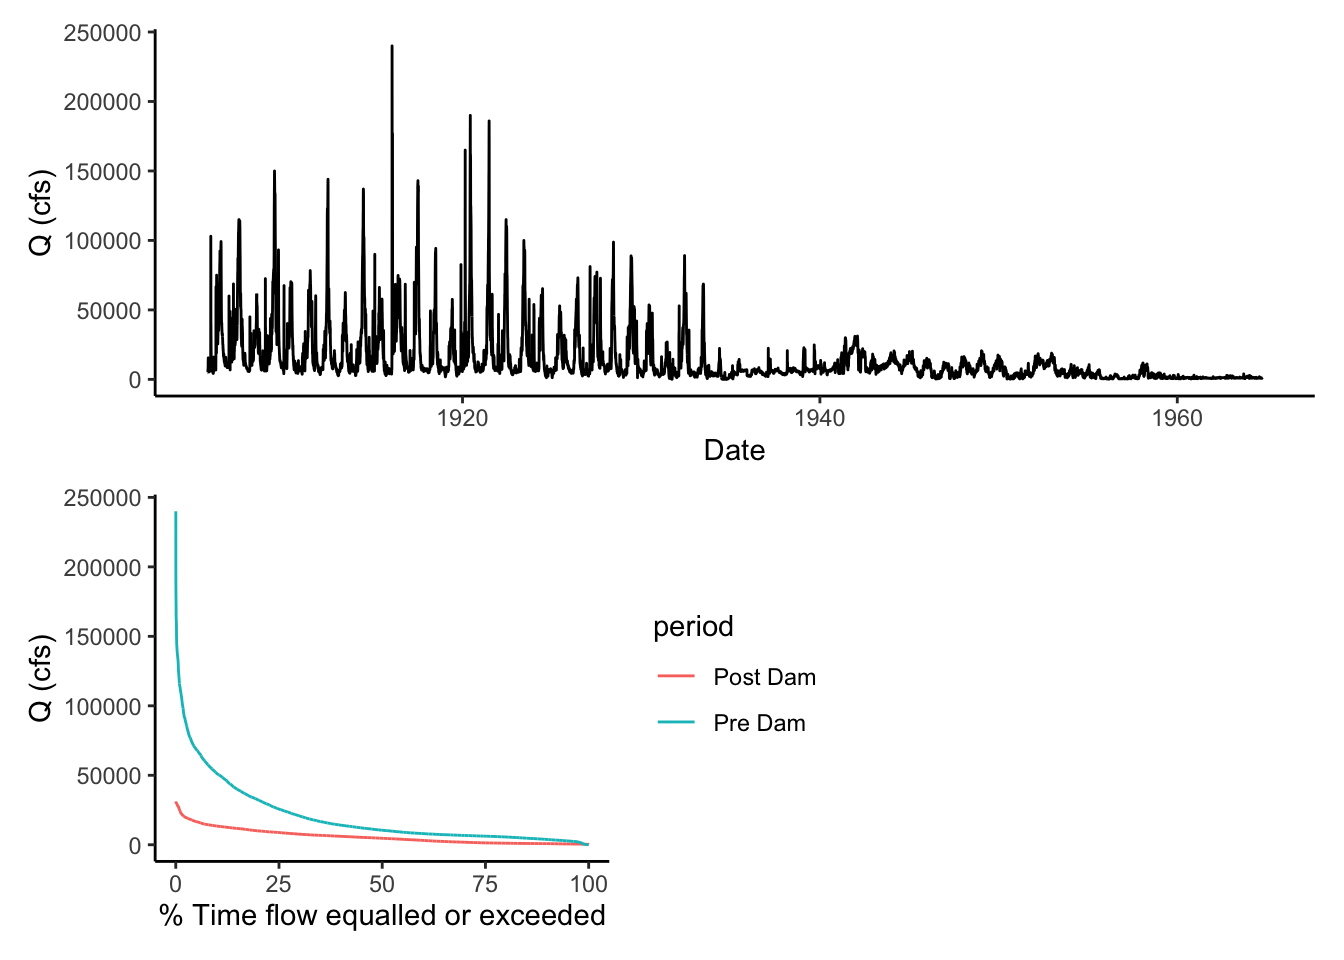
\includegraphics{Hydroinformatics_Bookdown_files/figure-latex/unnamed-chunk-94-1.pdf}

\hypertarget{challenge-examining-flow-regime-change-at-the-grand-canyon}{%
\section{Challenge: Examining flow regime change at the Grand Canyon}\label{challenge-examining-flow-regime-change-at-the-grand-canyon}}

The USGS Gage ``Colorado River at Yuma, AZ'' is below the Hoover dam. The Hoover Dam closed in 1936, changing the flow of the Colorado River below. Load average daily discharge data from 10-01-1905 to 10-01-1965 from the Yuma gage. Use a line plot of discharge and flow duration curves to examine the differences in discharge for the periods: 1905 - 1936, 1937 - 1965.

How does the FDC show the differences you observed in the line plot?

\begin{Shaded}
\begin{Highlighting}[]
\NormalTok{siteid }\OtherTok{\textless{}{-}} \StringTok{"09521000"}
\NormalTok{startDate }\OtherTok{\textless{}{-}} \StringTok{"1905{-}10{-}01"}
\NormalTok{endDate }\OtherTok{\textless{}{-}} \StringTok{"1965{-}10{-}01"}
\NormalTok{parameter }\OtherTok{\textless{}{-}} \StringTok{"00060"}

\NormalTok{WS }\OtherTok{\textless{}{-}} \FunctionTok{readNWISdv}\NormalTok{(siteid, parameter, startDate, endDate) }\SpecialCharTok{\%\textgreater{}\%} 
  \FunctionTok{renameNWISColumns}\NormalTok{() }\SpecialCharTok{\%\textgreater{}\%}
  \FunctionTok{mutate}\NormalTok{(}\AttributeTok{year =} \FunctionTok{year}\NormalTok{(Date)) }\SpecialCharTok{\%\textgreater{}\%}
  \FunctionTok{mutate}\NormalTok{(}\AttributeTok{period =} \FunctionTok{case\_when}\NormalTok{( year }\SpecialCharTok{\textless{}=} \DecValTok{1936} \SpecialCharTok{\textasciitilde{}} \StringTok{"Pre Dam"}\NormalTok{,}
\NormalTok{                             year }\SpecialCharTok{\textgreater{}} \DecValTok{1936}  \SpecialCharTok{\textasciitilde{}} \StringTok{"Post Dam"}\NormalTok{)) }\SpecialCharTok{\%\textgreater{}\%}
  \FunctionTok{group\_by}\NormalTok{(period) }\SpecialCharTok{\%\textgreater{}\%}
  \FunctionTok{mutate}\NormalTok{(}\AttributeTok{rank =} \FunctionTok{rank}\NormalTok{(}\SpecialCharTok{{-}}\NormalTok{Flow)) }\SpecialCharTok{\%\textgreater{}\%} 
  \FunctionTok{mutate}\NormalTok{(}\AttributeTok{P =} \DecValTok{100} \SpecialCharTok{*}\NormalTok{ (rank }\SpecialCharTok{/}\NormalTok{ (}\FunctionTok{length}\NormalTok{(Flow) }\SpecialCharTok{+} \DecValTok{1}\NormalTok{)))}

\NormalTok{flow }\OtherTok{\textless{}{-}} \FunctionTok{ggplot}\NormalTok{(WS, }\FunctionTok{aes}\NormalTok{(Date, Flow))}\SpecialCharTok{+}\CommentTok{\#, color = period))+}
  \FunctionTok{geom\_line}\NormalTok{()}\SpecialCharTok{+}
  \FunctionTok{ylab}\NormalTok{(}\StringTok{"Q (cfs)"}\NormalTok{)}

\NormalTok{fdc }\OtherTok{\textless{}{-}}\NormalTok{ WS }\SpecialCharTok{\%\textgreater{}\%} \FunctionTok{ggplot}\NormalTok{(}\FunctionTok{aes}\NormalTok{(}\AttributeTok{x =}\NormalTok{ P, }\AttributeTok{y =}\NormalTok{ Flow, }\AttributeTok{color =}\NormalTok{ period))}\SpecialCharTok{+}
  \FunctionTok{geom\_line}\NormalTok{()}\SpecialCharTok{+}
  \CommentTok{\#scale\_y\_log10()+}
  \FunctionTok{xlab}\NormalTok{(}\StringTok{"\% Time flow equalled or exceeded"}\NormalTok{)}\SpecialCharTok{+}
  \FunctionTok{ylab}\NormalTok{(}\StringTok{"Q (cfs)"}\NormalTok{)}

\NormalTok{flow }\SpecialCharTok{/}\NormalTok{ (fdc }\SpecialCharTok{+} \FunctionTok{plot\_spacer}\NormalTok{())}
\end{Highlighting}
\end{Shaded}

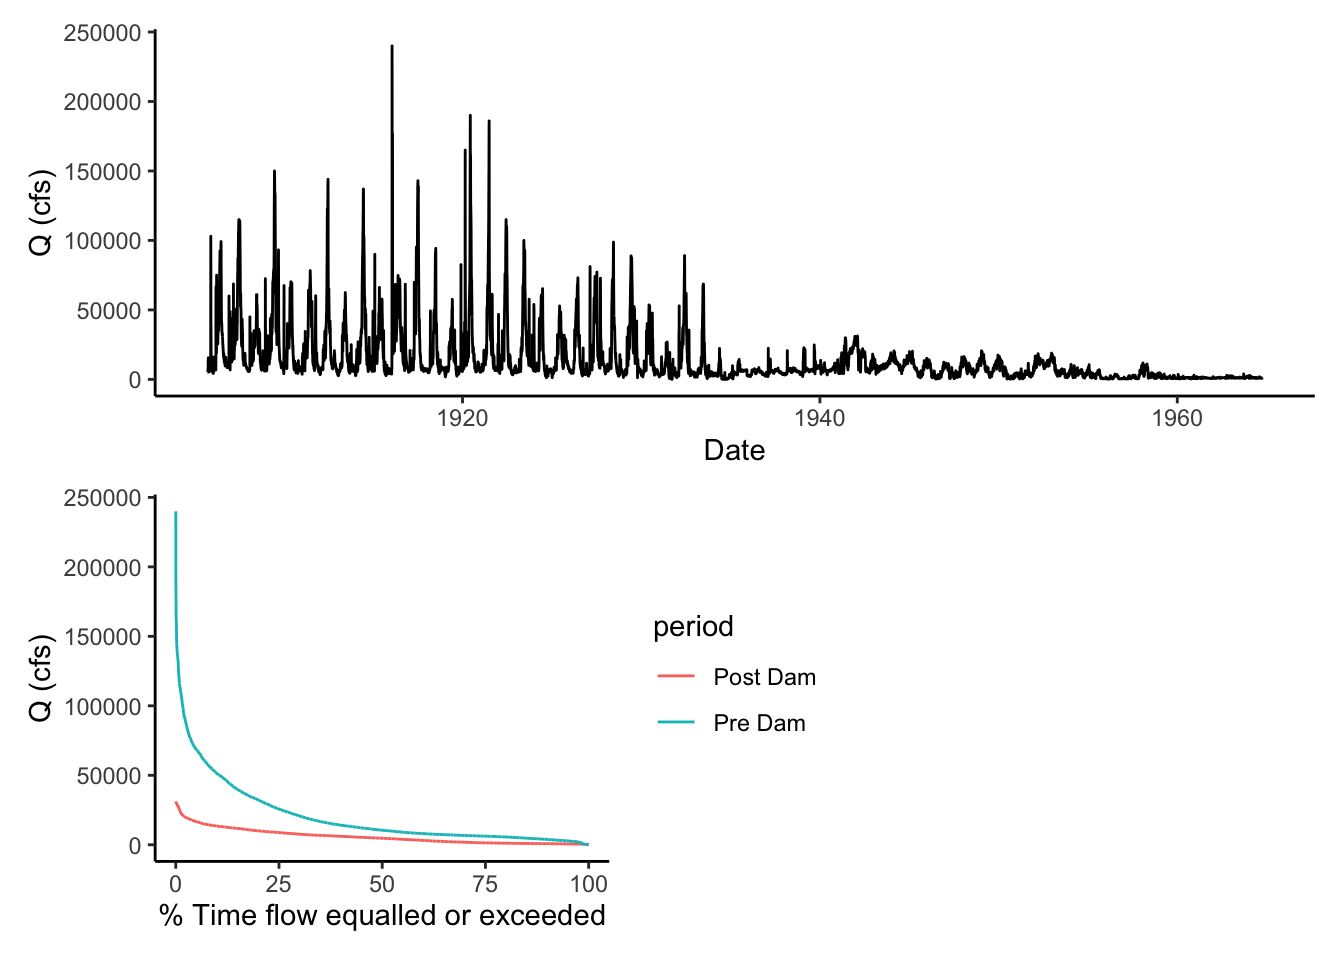
\includegraphics{Hydroinformatics_Bookdown_files/figure-latex/unnamed-chunk-95-1.pdf}
That's it! Next we will apply some of these principles to look at low-flow statistics.

\hypertarget{lfas}{%
\chapter{Low Flow Analysis}\label{lfas}}

Get this document and a version with empty code chunks at the template repository on github: \url{https://github.com/VT-Hydroinformatics/10-Low-Flow-Analysis}

\textbf{Pre-activity reading:}

\url{https://www.epa.gov/ceam/definition-and-characteristics-low-flows\#1Q10}

\textbf{Analysis based on:}

\url{https://github.com/DEQdsobota/Oregon7Q10/blob/master/R/Oregon7Q10.R}

\url{https://nepis.epa.gov/Exe/ZyPDF.cgi?Dockey=P100BK6P.txt}

\emph{Load packages for analysis. zoo will allow us to easily perform rolling means, and moments will allow easy calculation of skewness.}

\begin{Shaded}
\begin{Highlighting}[]
\FunctionTok{library}\NormalTok{(zoo)}
\FunctionTok{library}\NormalTok{(tidyverse)}
\FunctionTok{library}\NormalTok{(dataRetrieval)}
\FunctionTok{library}\NormalTok{(lubridate)}
\FunctionTok{library}\NormalTok{(moments)}

\FunctionTok{theme\_set}\NormalTok{(}\FunctionTok{theme\_classic}\NormalTok{())}
\end{Highlighting}
\end{Shaded}

\hypertarget{what-are-low-flow-statistics}{%
\section{What are low flow statistics?}\label{what-are-low-flow-statistics}}

Low flow design flows can be specified based on hydrological or biological data. Biological methods look more at water quality standards relevant to biota. The hydrologic method just looks at the statistical distribution of low flows over a period of time.

\begin{itemize}
\tightlist
\item
  Just from this simple definition, can you think of a management situation where it would make sense to use the biological method? the hydrologic method? What are the advantages to each?
\end{itemize}

We will focus on hydrologic methods. What a surprise! You will most frequently see low flow stats in the format of xQy. So for example 7Q10 or 1Q10 are common design flows. Let's look at the EPA definition of these and then break them down.

``The 1Q10 and 7Q10 are both hydrologically based design flows. The 1Q10 is the lowest 1-day average flow that occurs (on average) once every 10 years. The 7Q10 is the lowest 7-day average flow that occurs (on average) once every 10 years.'' -EPA \url{https://www.epa.gov/ceam/definition-and-characteristics-low-flows\#1Q10}

So the first number, \textbf{the 7 in 7Q10} is how many days we will average flow over to calculate the statistic. Why does does this matte? Why not always use a 1 day flow record?

Then the second number is the return-interval of the flow, or the probability that a flow of that magnitude or lower will occur any given year. \textbf{The 10 in 7Q10} means there is a 10 percent chance that the associated 7-day average flow or below will occur in any given year. Another way of saying this is that a flow of that magnitude or below occurs on average once every 10 years. \textbf{However} expressing it this way can be dangerous, especially with the opposite type of extreme flows: Floods. Why do you think it could be dangerous to say a flow of this magnitude or below will happen on average once every 10 years?

\textbf{So, to calculate a 7Q10} we need:
* 7-day mean-daily flows
* The minumum value per year of those 7-day mean-daily flows
* The return intervals of those flows minimum yearly flows

\textbf{Because a 7Q10 flow means}
* There is a 10\% chance (return interval = 10) that a river will have a average weekly flow of that level or below in a given year.

\hypertarget{get-data-1}{%
\section{Get data}\label{get-data-1}}

Let's get started on an example. We will calculate the 7Q10 low flow statistic for the Linville NC usgs gage (02138500) using daily discharge data from 1922-1984. (parameter = 00060)

\begin{Shaded}
\begin{Highlighting}[]
\NormalTok{siteno }\OtherTok{\textless{}{-}} \StringTok{"02138500"}
\NormalTok{startDate }\OtherTok{\textless{}{-}} \StringTok{"1922{-}01{-}01"}
\NormalTok{endDate }\OtherTok{\textless{}{-}} \StringTok{"1984{-}01{-}01"}
\NormalTok{parameter }\OtherTok{\textless{}{-}} \StringTok{"00060"}

\NormalTok{Qdat }\OtherTok{\textless{}{-}} \FunctionTok{readNWISdv}\NormalTok{(siteno, parameter, startDate, endDate) }\SpecialCharTok{\%\textgreater{}\%} 
  \FunctionTok{renameNWISColumns}\NormalTok{()}
\end{Highlighting}
\end{Shaded}

\hypertarget{create-the-x-days-average-flow-record}{%
\section{Create the X days average flow record}\label{create-the-x-days-average-flow-record}}

Remember the 7 in 7Q10 means we are looking at the 7-day average flow. We just have daily values from the USGS gage, so we need to create this data record.

To do this we will calculate a rolling average, also called a moving-window average. This just means you grab the first 7 days, average them, then move the window of the days you are averaging forward a day, and average again\ldots{} all the way through the record.

For your rolling mean you can have the window look forward, backward, or forward and backward. For example, a forward window takes the average of X number of records and places the value at the beginning. Backward places that value at the end, and both would put it in the middle. In the function we will use to do this, forward is a left align, backward is right align, and both is centered.

\textbf{For example}

\begin{quote}
data window = 1, 2, 3, 4, 5 (lots of values before and after this)
\end{quote}

\begin{quote}
mean = 3
\end{quote}

\begin{quote}
forward window/left align: 3, NA, NA, NA, NA
\end{quote}

\begin{quote}
backward window/right align: NA, NA, NA, NA, 3
\end{quote}

\begin{quote}
both/center align: NA, NA, 3, NA, NA
\end{quote}

We could certainly set up some code to calculate this, but there is a nice and fast function in the zoo package for calculating rolling means.

As we write the code to do this analysis, we are going to keep in mind that we may want to calculate a different type of low flow, like a 1Q10, so we are going to store the x and y of the xQy low flow statistic as objects rather than including them several places in the code. That way we can just change them in one place and run the analysis to compute a different statistic.

\begin{Shaded}
\begin{Highlighting}[]
\CommentTok{\#set x and y for xQy design flow}
\NormalTok{Xday }\OtherTok{\textless{}{-}} \DecValTok{7}
\NormalTok{YrecInt }\OtherTok{\textless{}{-}} \DecValTok{10}

\CommentTok{\#X day rolling mean, don\textquotesingle{}t fill the ends of the timeseries,}
\CommentTok{\#don\textquotesingle{}t ignore NAs, use a backward{-}looking window (right align)}
\NormalTok{Qdat }\OtherTok{\textless{}{-}}\NormalTok{ Qdat }\SpecialCharTok{\%\textgreater{}\%} \FunctionTok{mutate}\NormalTok{(}\AttributeTok{xdaymean =} \FunctionTok{rollmean}\NormalTok{(Flow, }
\NormalTok{                                            Xday, }
                                            \AttributeTok{fill =} \ConstantTok{NA}\NormalTok{, }
                                            \AttributeTok{na.rm =}\NormalTok{ F, }
                                            \AttributeTok{align =} \StringTok{"right"}\NormalTok{))}
\end{Highlighting}
\end{Shaded}

\hypertarget{look-at-what-a-rolling-mean-does.}{%
\section{Look at what a rolling mean does.}\label{look-at-what-a-rolling-mean-does.}}

We just added a new column with the rolling mean, so let's plot it and see what it did to the discharge record.

Let's look at June-August 1960. You can't see too well what is going on in the full record.

\begin{Shaded}
\begin{Highlighting}[]
\NormalTok{Qdat }\SpecialCharTok{\%\textgreater{}\%} 
  \FunctionTok{filter}\NormalTok{(Date }\SpecialCharTok{\textgreater{}} \FunctionTok{mdy}\NormalTok{(}\StringTok{"06{-}01{-}1960"}\NormalTok{) }\SpecialCharTok{\&}\NormalTok{ Date }\SpecialCharTok{\textless{}} \FunctionTok{mdy}\NormalTok{(}\StringTok{"08{-}01{-}1960"}\NormalTok{)) }\SpecialCharTok{\%\textgreater{}\%}
  \FunctionTok{ggplot}\NormalTok{(}\FunctionTok{aes}\NormalTok{(Date, Flow, }\AttributeTok{color =} \StringTok{"daily"}\NormalTok{))}\SpecialCharTok{+}
    \FunctionTok{geom\_line}\NormalTok{()}\SpecialCharTok{+}
    \FunctionTok{geom\_line}\NormalTok{(}\FunctionTok{aes}\NormalTok{(}\AttributeTok{x =}\NormalTok{ Date, }\AttributeTok{y =}\NormalTok{ xdaymean, }\AttributeTok{color =} \StringTok{"rolling mean"}\NormalTok{))}
\end{Highlighting}
\end{Shaded}

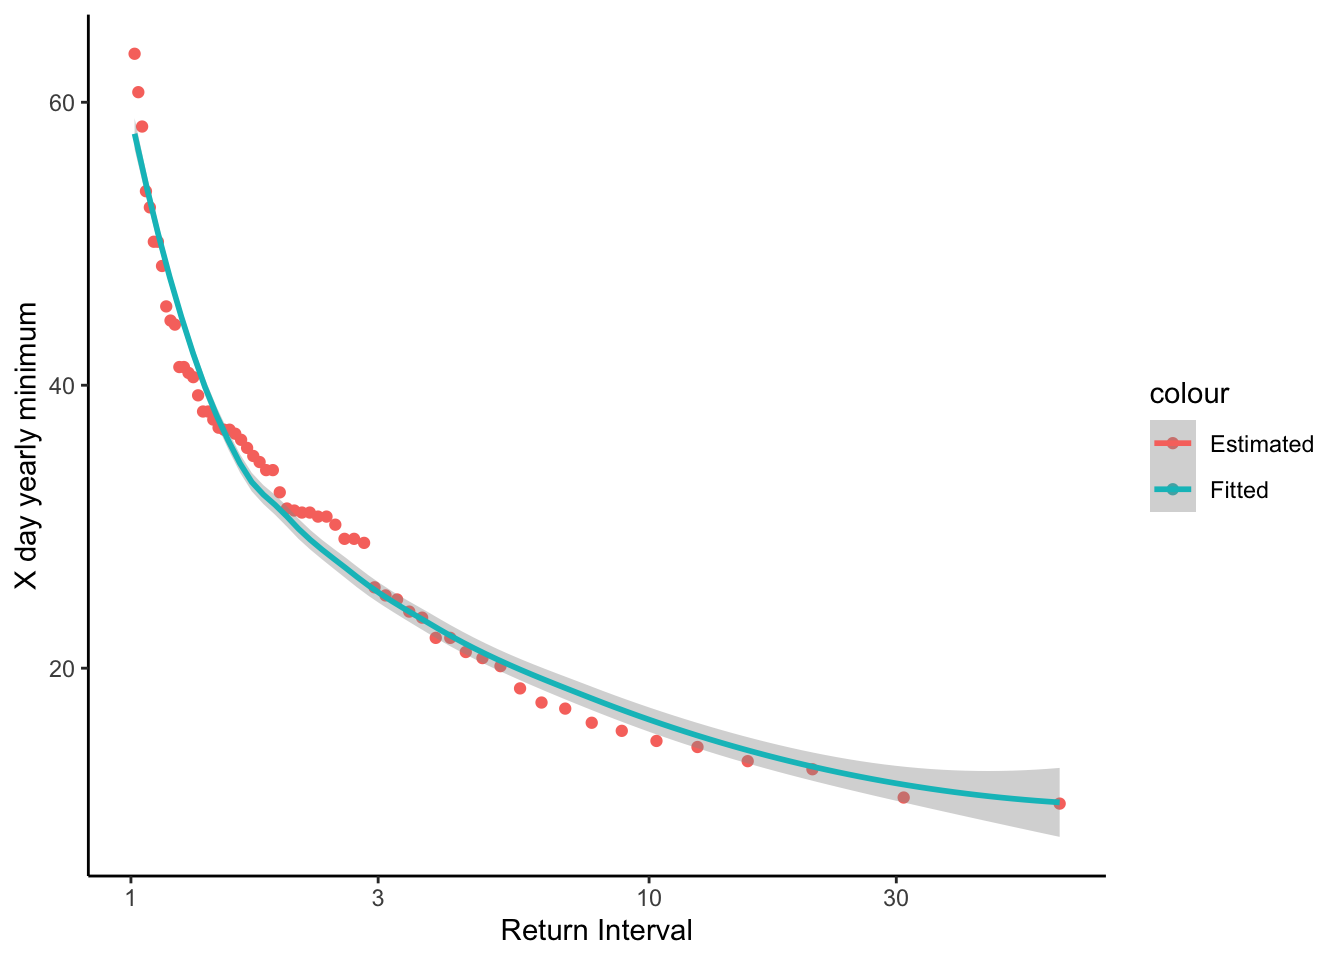
\includegraphics{Hydroinformatics_Bookdown_files/figure-latex/unnamed-chunk-99-1.pdf}

\hypertarget{calculate-yearly-minimums}{%
\section{Calculate yearly minimums}\label{calculate-yearly-minimums}}

Okay, we have our X-day rolling mean. Now we need to calculate the probability that a given magnitude flow or below will happen in a given year. Because we are concerned with \emph{a given year} we need the lowest flow per year.

We will calculate minimum flow per year by creating a \emph{Year} column, grouping by that column, and using the summarize function to calculate the minimum flow per year. The code we are going to write will also drop any years that are missing too much data by dropping years missing 10\% or more days.

\begin{Shaded}
\begin{Highlighting}[]
\CommentTok{\#missing less than 10\% of each year and 10\% or fewer NAs}
\NormalTok{QyearlyMins }\OtherTok{\textless{}{-}}\NormalTok{ Qdat }\SpecialCharTok{\%\textgreater{}\%} \FunctionTok{mutate}\NormalTok{(}\AttributeTok{year =} \FunctionTok{year}\NormalTok{(Date)) }\SpecialCharTok{\%\textgreater{}\%}
                        \FunctionTok{group\_by}\NormalTok{(year) }\SpecialCharTok{\%\textgreater{}\%}
                        \FunctionTok{summarize}\NormalTok{(}\AttributeTok{minQ =} \FunctionTok{min}\NormalTok{(xdaymean, }\AttributeTok{na.rm =}\NormalTok{ T), }
                                  \AttributeTok{lenDat =} \FunctionTok{length}\NormalTok{(Flow),}
                                  \AttributeTok{lenNAs =} \FunctionTok{sum}\NormalTok{(}\FunctionTok{is.na}\NormalTok{(xdaymean))) }\SpecialCharTok{\%\textgreater{}\%}
                        \FunctionTok{filter}\NormalTok{(lenDat }\SpecialCharTok{\textgreater{}} \DecValTok{328} \SpecialCharTok{\&}\NormalTok{ lenNAs }\SpecialCharTok{/}\NormalTok{ lenDat }\SpecialCharTok{\textless{}} \FloatTok{0.1}\NormalTok{) }
\end{Highlighting}
\end{Shaded}

\hypertarget{calculate-return-interval}{%
\section{Calculate return interval}\label{calculate-return-interval}}

Now that we have an object that contains our yearly minimum flows, we can calculate the return interval as

\(Return Interval = (n + 1) / rank\)

Where n is the number of records in the data (number of years) and rank is the rank of each year's low flow (lowest flow = rank 1 and so on). We can calculate the rank with the rank() function in base R. In the rank function we will specify that in the case of a tie, the first value gets the lower rank using ties.method = ``first''.

We can then transform that to an exceedence probability as

\(Exceedence Probability = 1 / Return Interval\)

Once we calculate the return interval and exceedence probability we will plot the return interval against the minimum discharge.

\begin{Shaded}
\begin{Highlighting}[]
\CommentTok{\# add rank column and return interval column}
\NormalTok{QyearlyMins }\OtherTok{\textless{}{-}}\NormalTok{ QyearlyMins }\SpecialCharTok{\%\textgreater{}\%} 
                \FunctionTok{mutate}\NormalTok{(}\AttributeTok{rank =} \FunctionTok{rank}\NormalTok{(minQ, }\AttributeTok{ties.method =} \StringTok{"first"}\NormalTok{)) }\SpecialCharTok{\%\textgreater{}\%}
                \FunctionTok{mutate}\NormalTok{(}\AttributeTok{ReturnInterval =}\NormalTok{ (}\FunctionTok{length}\NormalTok{(rank) }\SpecialCharTok{+} \DecValTok{1}\NormalTok{)}\SpecialCharTok{/}\NormalTok{rank) }\SpecialCharTok{\%\textgreater{}\%}
                \FunctionTok{mutate}\NormalTok{(}\AttributeTok{ExceedProb =} \DecValTok{1} \SpecialCharTok{/}\NormalTok{ ReturnInterval)}
      
\FunctionTok{ggplot}\NormalTok{(QyearlyMins, }\FunctionTok{aes}\NormalTok{(}\AttributeTok{x =}\NormalTok{ ReturnInterval, }\AttributeTok{y =}\NormalTok{ minQ))}\SpecialCharTok{+}
  \FunctionTok{geom\_point}\NormalTok{()}
\end{Highlighting}
\end{Shaded}

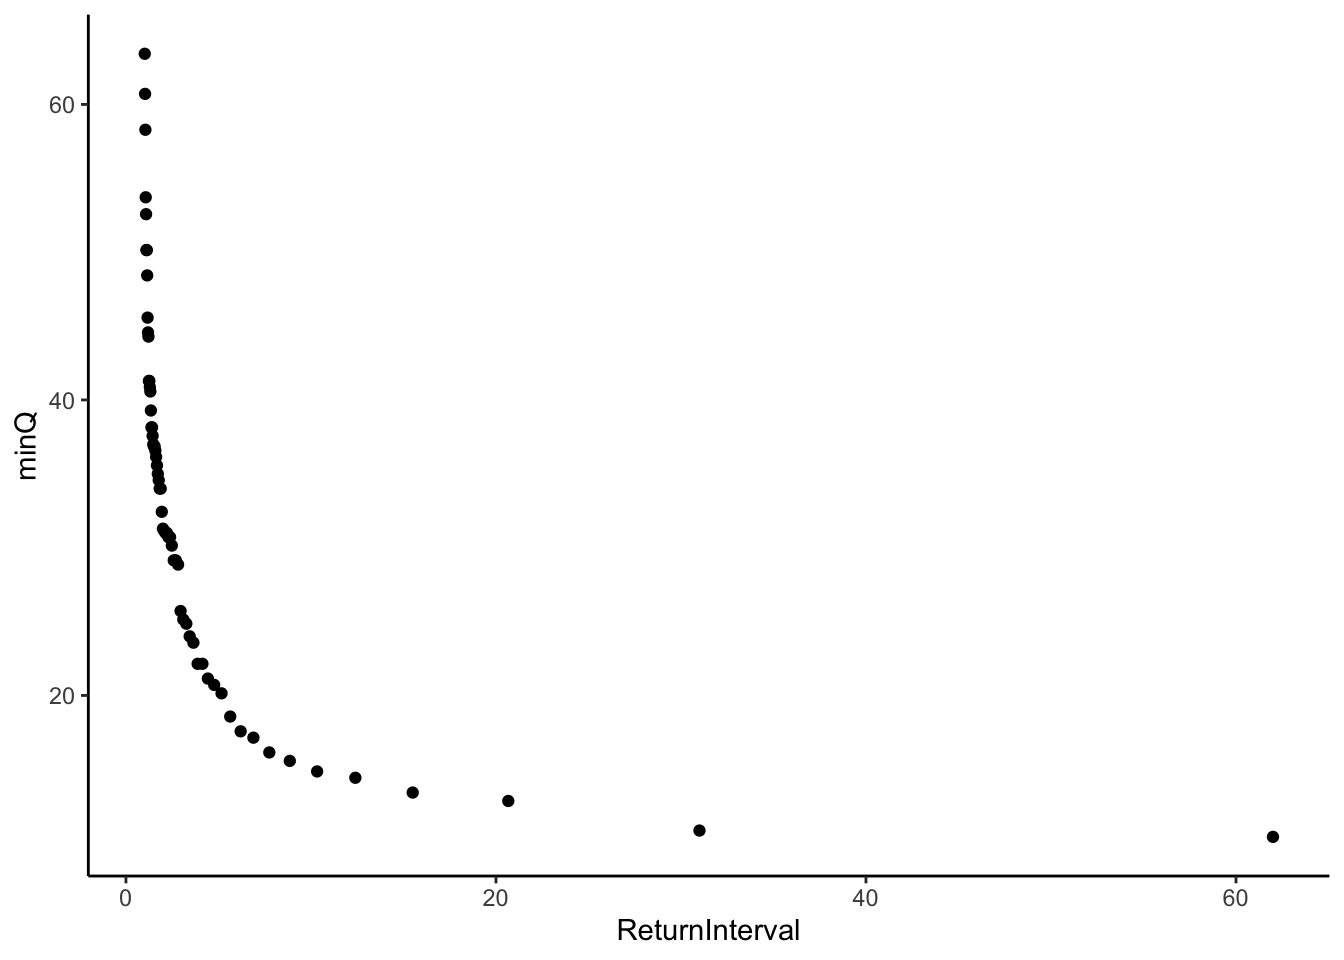
\includegraphics{Hydroinformatics_Bookdown_files/figure-latex/unnamed-chunk-101-1.pdf}

\textbf{Challenge question} How is this similar to a flow duration curve? Could you make a ``flow duration curve'' from these data? What would it tell you?

\begin{Shaded}
\begin{Highlighting}[]
\FunctionTok{ggplot}\NormalTok{(QyearlyMins, }\FunctionTok{aes}\NormalTok{(}\AttributeTok{x =}\NormalTok{ ExceedProb, }\AttributeTok{y =}\NormalTok{ minQ))}\SpecialCharTok{+}
  \FunctionTok{geom\_point}\NormalTok{()}
\end{Highlighting}
\end{Shaded}

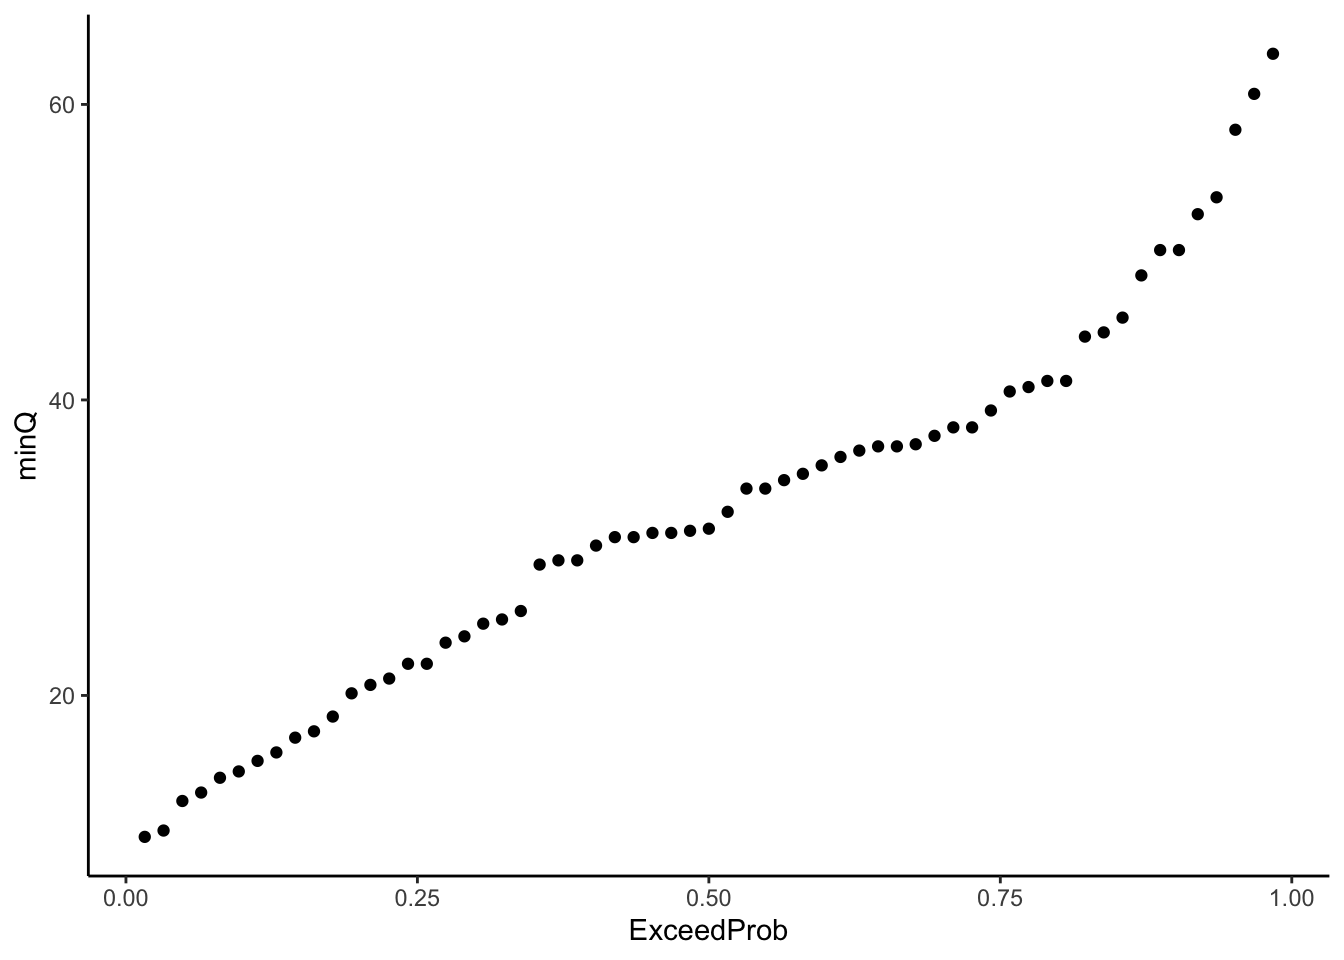
\includegraphics{Hydroinformatics_Bookdown_files/figure-latex/unnamed-chunk-102-1.pdf}

\hypertarget{fit-to-pearson-type-iii-distribution}{%
\section{Fit to Pearson Type III distribution}\label{fit-to-pearson-type-iii-distribution}}

Source for these calculations:
\url{https://water.usgs.gov/osw/bulletin17b/dl_flow.pdf}

We now have everything we need to calculate what the 10-year return interval flow is (the 0.1 probability flow). To do this, we have to fit a distribution to our data and then use that fitted distribution to predict the value of the 10-year return interval flow.

This may sound a little complex, but let's think about it this way:

\begin{itemize}
\tightlist
\item
  You have some data, let's say: heights of students at Virginia Tech
\item
  You did some tests on it and know it is a normal distribution
\item
  If you measure the mean and standard deviation of that distribution, you could create a ``fitted'' representation of your distrubtion by generating a normal distribution with the same mean and standard deviation with the rnorm() function.
\item
  Now you could plot that fitted, synthetic distribution as an ECDF and read the plot to determine, say, 10\% of students (0.1 probability) are at or above what height?
\end{itemize}

Assume the average height from your data was 65 inches and the standard deviation was 6 inches (this is 100\% made up), let's look at it.

\begin{Shaded}
\begin{Highlighting}[]
\NormalTok{fitteddistribution }\OtherTok{\textless{}{-}} \FunctionTok{rnorm}\NormalTok{(}\DecValTok{1000}\NormalTok{, }\AttributeTok{mean =} \DecValTok{65}\NormalTok{, }\AttributeTok{sd =} \DecValTok{6}\NormalTok{) }\SpecialCharTok{\%\textgreater{}\%}
  \FunctionTok{as\_tibble}\NormalTok{()}

\FunctionTok{ggplot}\NormalTok{(fitteddistribution, }\FunctionTok{aes}\NormalTok{(}\AttributeTok{x =}\NormalTok{ value))}\SpecialCharTok{+}
  \FunctionTok{stat\_ecdf}\NormalTok{()}\SpecialCharTok{+}
  \FunctionTok{xlab}\NormalTok{(}\StringTok{"height (in)"}\NormalTok{)}\SpecialCharTok{+}
  \FunctionTok{ylab}\NormalTok{(}\StringTok{"probability"}\NormalTok{)}
\end{Highlighting}
\end{Shaded}

\includegraphics{Hydroinformatics_Bookdown_files/figure-latex/unnamed-chunk-103-1.pdf}

To get our 10 year return period (0.1 exceedence probability) we are going to do the same thing, except we know the distribution of the data isn't normal, so we have to use a different distribution.

There are a bunch of ``extreme value'' distributions used in these type of analyses. When we talk about floods we will use the Gumbel distribution, for example. For this type of analysis, it is common to use the Pearson Type III distribution.

When we used the normal distribution example, we let R produce the distribution that fit our data. In this case we will use an equation that describes the Person Type III distribution. To predict flow at a given recurrence interval we will need the mean of the logged discharges (Xbar), the frequency factor (K), the standard deviation of the log discharges (S), skewness (g), and the standard normal variate (z). We will first compute this for all of the values in our dataset to see how the fitted values fit our calculated values.

\textbf{Pearson Type III: Frequency Factor method}

\(Flow = 10^(Xbar + KS)\)

where:

Xbar = mean of the log discharge you are investigating

K = frequency factor

S = standard deviation of log discharges

\textbf{Frequency Factor}

\(K = (2 / g) * ((1 +( g * z)) / 6 - ((g ^ 2) / 36)) ^ 3 - 1)\)

\textbf{Skewness}

g = skewness() from moments package

\textbf{Standard normal variate}

\(z = 4.91 * ((1 / y) ^ {0.14} - (1 - (1 / y)) ^ {0.14})\)

y = recurrence interval

\begin{Shaded}
\begin{Highlighting}[]
\CommentTok{\#Measures of the distribution}
\NormalTok{Xbar }\OtherTok{\textless{}{-}} \FunctionTok{mean}\NormalTok{(}\FunctionTok{log10}\NormalTok{(QyearlyMins}\SpecialCharTok{$}\NormalTok{minQ))}
\NormalTok{S    }\OtherTok{\textless{}{-}} \FunctionTok{sd}\NormalTok{(}\FunctionTok{log10}\NormalTok{(QyearlyMins}\SpecialCharTok{$}\NormalTok{minQ))}
\NormalTok{g    }\OtherTok{\textless{}{-}} \FunctionTok{skewness}\NormalTok{(}\FunctionTok{log10}\NormalTok{(QyearlyMins}\SpecialCharTok{$}\NormalTok{minQ))}
 
\CommentTok{\#calculate z, K, to plot the fitted Pearson Type III}
\NormalTok{QyearlyMins }\OtherTok{\textless{}{-}}\NormalTok{ QyearlyMins }\SpecialCharTok{\%\textgreater{}\%} 
  \FunctionTok{mutate}\NormalTok{(}\AttributeTok{z =} \FloatTok{4.91} \SpecialCharTok{*}\NormalTok{ ((}\DecValTok{1} \SpecialCharTok{/}\NormalTok{ ReturnInterval) }\SpecialCharTok{\^{}} \FloatTok{0.14} \SpecialCharTok{{-}}\NormalTok{ (}\DecValTok{1} \SpecialCharTok{{-}} \DecValTok{1} \SpecialCharTok{/}\NormalTok{ ReturnInterval) }\SpecialCharTok{\^{}} \FloatTok{0.14}\NormalTok{)) }\SpecialCharTok{\%\textgreater{}\%}
  \FunctionTok{mutate}\NormalTok{(}\AttributeTok{K =}\NormalTok{ (}\DecValTok{2} \SpecialCharTok{/}\NormalTok{ g) }\SpecialCharTok{*}\NormalTok{ (((}\DecValTok{1} \SpecialCharTok{+}\NormalTok{ (g }\SpecialCharTok{*}\NormalTok{ z) }\SpecialCharTok{/} \DecValTok{6} \SpecialCharTok{{-}}\NormalTok{ (g }\SpecialCharTok{\^{}} \DecValTok{2}\NormalTok{) }\SpecialCharTok{/} \DecValTok{36}\NormalTok{) }\SpecialCharTok{\^{}} \DecValTok{3}\NormalTok{) }\SpecialCharTok{{-}} \DecValTok{1}\NormalTok{) ) }\SpecialCharTok{\%\textgreater{}\%}
  \FunctionTok{mutate}\NormalTok{(}\AttributeTok{Qfit =} \DecValTok{10}\SpecialCharTok{\^{}}\NormalTok{(Xbar }\SpecialCharTok{+}\NormalTok{ (K }\SpecialCharTok{*}\NormalTok{ S)))}
\end{Highlighting}
\end{Shaded}

Let's look our results and see how they fit. Plot the return interval on the x axis and flow on the y. Plot minQ, the minimum Q data, and Qfit, the data from the the model fit.

\begin{Shaded}
\begin{Highlighting}[]
\NormalTok{QyearlyMins }\SpecialCharTok{\%\textgreater{}\%} 
  \FunctionTok{ggplot}\NormalTok{(}\FunctionTok{aes}\NormalTok{(}\AttributeTok{x =}\NormalTok{ ReturnInterval, }\AttributeTok{y =}\NormalTok{ minQ, }\AttributeTok{color =} \StringTok{"Estimated"}\NormalTok{))}\SpecialCharTok{+}
  \FunctionTok{geom\_point}\NormalTok{()}\SpecialCharTok{+}
  \FunctionTok{geom\_line}\NormalTok{(}\FunctionTok{aes}\NormalTok{(}\AttributeTok{x =}\NormalTok{ ReturnInterval, }\AttributeTok{y =}\NormalTok{ Qfit, }\AttributeTok{color =} \StringTok{"Fitted"}\NormalTok{))}\SpecialCharTok{+}
  \FunctionTok{theme\_classic}\NormalTok{()}\SpecialCharTok{+}
  \FunctionTok{scale\_x\_log10}\NormalTok{()}\SpecialCharTok{+}
  \FunctionTok{ylab}\NormalTok{(}\StringTok{"X day yearly minimum"}\NormalTok{)}\SpecialCharTok{+}
  \FunctionTok{xlab}\NormalTok{(}\StringTok{"Return Interval"}\NormalTok{)}
\end{Highlighting}
\end{Shaded}

\includegraphics{Hydroinformatics_Bookdown_files/figure-latex/unnamed-chunk-105-1.pdf}

Above we calculated z, K and the flow for each return interval in our data record to see how the distribution fit our data. We can see it fits quite well.

We can use the same calculations as we used on the entire record to calculate a specific return period of interest. In our case, the 10 year return period for the 7Q10.

We will set y equal to YrecInt, which we set above. This way we can just change it at the top of the code to run whatever xQy metric we want.

\begin{Shaded}
\begin{Highlighting}[]
\CommentTok{\#xQy ei: 7Q10}
\NormalTok{y }\OtherTok{=}\NormalTok{ YrecInt}

\CommentTok{\#Find these values based on established relationships}
\NormalTok{z    }\OtherTok{\textless{}{-}} \FloatTok{4.91} \SpecialCharTok{*}\NormalTok{ ((}\DecValTok{1} \SpecialCharTok{/}\NormalTok{ y) }\SpecialCharTok{\^{}} \FloatTok{0.14} \SpecialCharTok{{-}}\NormalTok{ (}\DecValTok{1} \SpecialCharTok{{-}} \DecValTok{1} \SpecialCharTok{/}\NormalTok{ y) }\SpecialCharTok{\^{}} \FloatTok{0.14}\NormalTok{)}
\NormalTok{K    }\OtherTok{\textless{}{-}}\NormalTok{ (}\DecValTok{2} \SpecialCharTok{/}\NormalTok{ g) }\SpecialCharTok{*}\NormalTok{ (((}\DecValTok{1} \SpecialCharTok{+}\NormalTok{ (g }\SpecialCharTok{*}\NormalTok{ z) }\SpecialCharTok{/} \DecValTok{6} \SpecialCharTok{{-}}\NormalTok{ (g }\SpecialCharTok{\^{}} \DecValTok{2}\NormalTok{) }\SpecialCharTok{/} \DecValTok{36}\NormalTok{) }\SpecialCharTok{\^{}} \DecValTok{3}\NormalTok{) }\SpecialCharTok{{-}} \DecValTok{1}\NormalTok{) }

\NormalTok{PearsonxQy }\OtherTok{\textless{}{-}} \DecValTok{10}\SpecialCharTok{\^{}}\NormalTok{(Xbar }\SpecialCharTok{+}\NormalTok{ K }\SpecialCharTok{*}\NormalTok{ S)}
\end{Highlighting}
\end{Shaded}

So, our 7Q10 flow in cfs for this gage is\ldots.

\begin{Shaded}
\begin{Highlighting}[]
\CommentTok{\#Low flow stat (7Q10 in exercise)}
\NormalTok{PearsonxQy}
\end{Highlighting}
\end{Shaded}

\begin{verbatim}
## [1] 16.70488
\end{verbatim}

\hypertarget{distribution-free-method}{%
\section{Distribution-free method}\label{distribution-free-method}}

We won't go over this in the same detail, but the xQy flow can also be calculated using a formula that does not assume a specific distribution. The expression, and code to perform it, is below.

\textbf{The expression for xQy is:}

\(xQy = (1-e) X(m1) + eX(m2)\)

where:
{[} {]} indicates the value is truncated

\(X(m)\) = the m-th lowest annual low flow of record

\(m1 = [(n+1)/y]\)

\(m2 = [(n+l)/y] + 1\)

\([z]\) = the largest integer less than or equal to z

\(e = (n+l)/y - [(n+l)/y]\)

This method is only appropriate when the desired return period is less than n/5 years

\begin{Shaded}
\begin{Highlighting}[]
\NormalTok{x }\OtherTok{\textless{}{-}}\NormalTok{ Xday}
\NormalTok{y }\OtherTok{\textless{}{-}}\NormalTok{ YrecInt}
\NormalTok{n }\OtherTok{\textless{}{-}} \FunctionTok{length}\NormalTok{(QyearlyMins}\SpecialCharTok{$}\NormalTok{minQ)}

\NormalTok{m1 }\OtherTok{\textless{}{-}} \FunctionTok{trunc}\NormalTok{((n }\SpecialCharTok{+} \DecValTok{1}\NormalTok{)}\SpecialCharTok{/}\NormalTok{y)}
\NormalTok{m2 }\OtherTok{\textless{}{-}} \FunctionTok{trunc}\NormalTok{(((n }\SpecialCharTok{+} \DecValTok{1}\NormalTok{)}\SpecialCharTok{/}\NormalTok{y) }\SpecialCharTok{+} \DecValTok{1}\NormalTok{)}

\NormalTok{e }\OtherTok{\textless{}{-}}\NormalTok{ ((n }\SpecialCharTok{+} \DecValTok{1}\NormalTok{)}\SpecialCharTok{/}\NormalTok{y) }\SpecialCharTok{{-}}\NormalTok{ m1}

\NormalTok{Xm1 }\OtherTok{\textless{}{-}}\NormalTok{ QyearlyMins}\SpecialCharTok{$}\NormalTok{minQ[QyearlyMins}\SpecialCharTok{$}\NormalTok{rank }\SpecialCharTok{==}\NormalTok{ m1]}
\NormalTok{Xm2 }\OtherTok{\textless{}{-}}\NormalTok{ QyearlyMins}\SpecialCharTok{$}\NormalTok{minQ[QyearlyMins}\SpecialCharTok{$}\NormalTok{rank }\SpecialCharTok{==}\NormalTok{ m2]}

\NormalTok{DFxQy }\OtherTok{\textless{}{-}}\NormalTok{ (}\DecValTok{1}\SpecialCharTok{{-}}\NormalTok{e) }\SpecialCharTok{*}\NormalTok{ Xm1 }\SpecialCharTok{+}\NormalTok{ e }\SpecialCharTok{*}\NormalTok{ Xm2}

\NormalTok{DFxQy}
\end{Highlighting}
\end{Shaded}

\begin{verbatim}
## [1] 15
\end{verbatim}

\hypertarget{floods}{%
\chapter{Flood Frequency Analysis and Creating Functions}\label{floods}}

\hypertarget{template-repository}{%
\section{Template Repository}\label{template-repository}}

The following activity is available as a template github repository at the following link: \url{https://github.com/VT-Hydroinformatics/11-Flood-Frequency-and-Functions}

\hypertarget{introduction-2}{%
\section{Introduction}\label{introduction-2}}

This methods for this chapter are adapted from the following activity:
\url{https://serc.carleton.edu/hydromodules/steps/166250.html}

After working with Flow Duration Curves (FDCs) and performing a low flow analysis, we now understand all the concepts necessary to perform a flood frequency analysis. In this chapter we will perform a flood frequency analysis using a Gumbel extreme value distribution and then write our own function that will return the return interval of magnitude flow we want! At the end of the chapter you will be challenged to write a function that performs a flood frequency analysis for any USGS gage.

First we will load the tidyverse and dataRetrieval packages and the set the theme for our plots.

\begin{Shaded}
\begin{Highlighting}[]
\FunctionTok{library}\NormalTok{(tidyverse)}
\FunctionTok{library}\NormalTok{(dataRetrieval)}

\FunctionTok{theme\_set}\NormalTok{(}\FunctionTok{theme\_classic}\NormalTok{())}
\end{Highlighting}
\end{Shaded}

\hypertarget{download-and-plot-peak-flow-data}{%
\section{Download and plot peak flow data}\label{download-and-plot-peak-flow-data}}

Next, download the yearly peakflow data from USGS dataRetrieval using the readNWISpeak() function. We don't have to create our own yearly values like we did in the low flow analysis. This function just returns the highest flow for each year.

Download the data for the New River at Radford starting in 1945.

Then make a plot of the peak flow for each year.

\begin{Shaded}
\begin{Highlighting}[]
\NormalTok{radford }\OtherTok{\textless{}{-}} \StringTok{"03171000"}

\NormalTok{peakflows }\OtherTok{\textless{}{-}} \FunctionTok{readNWISpeak}\NormalTok{(radford, }\AttributeTok{startDate =} \StringTok{"1945{-}01{-}01"}\NormalTok{)}

\FunctionTok{ggplot}\NormalTok{(peakflows, }\FunctionTok{aes}\NormalTok{(peak\_dt, peak\_va))}\SpecialCharTok{+}
  \FunctionTok{geom\_point}\NormalTok{()}
\end{Highlighting}
\end{Shaded}

\includegraphics{Hydroinformatics_Bookdown_files/figure-latex/unnamed-chunk-110-1.pdf}

\hypertarget{compute-ranks-for-peak-flows}{%
\section{Compute ranks for peak flows}\label{compute-ranks-for-peak-flows}}

As with the couple previous chapters, the next step is to create a column that contains the ranks of each flow in the record. Create a column that has the rank of each flow, with the highest flow ranked \#1. Use select() to trim your dataset to just the peak data, peak values, and ranks columns.

Make the plot from the last code chunk again but color the points by rank to check that this worked.
Also, look at the data through the environment tab in rstudio or using head() to double check.

\begin{Shaded}
\begin{Highlighting}[]
\CommentTok{\#create rank column (minus flips the ranking)}
\CommentTok{\#then clean it up, pull out only peak value, date, rank}
\NormalTok{peakflows }\OtherTok{\textless{}{-}}\NormalTok{ peakflows }\SpecialCharTok{\%\textgreater{}\%} \FunctionTok{mutate}\NormalTok{(}\AttributeTok{ranks =} \FunctionTok{rank}\NormalTok{(}\SpecialCharTok{{-}}\NormalTok{peak\_va)) }\SpecialCharTok{\%\textgreater{}\%}
              \FunctionTok{select}\NormalTok{(peak\_dt, peak\_va, ranks)}

\CommentTok{\#look at it}
\FunctionTok{ggplot}\NormalTok{(peakflows, }\FunctionTok{aes}\NormalTok{(peak\_dt, peak\_va, }\AttributeTok{color =}\NormalTok{ ranks))}\SpecialCharTok{+}
  \FunctionTok{geom\_point}\NormalTok{()}
\end{Highlighting}
\end{Shaded}

\includegraphics{Hydroinformatics_Bookdown_files/figure-latex/unnamed-chunk-111-1.pdf}

\begin{Shaded}
\begin{Highlighting}[]
\FunctionTok{head}\NormalTok{(peakflows)}
\end{Highlighting}
\end{Shaded}

\begin{verbatim}
##      peak_dt peak_va ranks
## 1 1945-09-18   62700  14.0
## 2 1946-01-08   44400  34.0
## 3 1947-01-20   34500  48.5
## 4 1948-02-14   34500  48.5
## 5 1949-08-29   40800  38.0
## 6 1949-11-02   15200  73.0
\end{verbatim}

\hypertarget{calculate-exceedance-probability-and-return-period}{%
\section{Calculate exceedance probability and return period}\label{calculate-exceedance-probability-and-return-period}}

Now we need to calculate the exceedance probability and return interval for each value in our data. For flood frequency analysis, it is common to use the Gringorten plotting position formula:

\begin{figure}
\centering
\includegraphics{images/plottingposition.png}
\caption{Plotting Position Formula}
\end{figure}

qi = Exceedance probability

N = Number of observations in your record

i = Rank of specific observation, i = 1 is the largest, i = N is the smallest.

a = constant for estimation = 0.44

\begin{center}\rule{0.5\linewidth}{0.5pt}\end{center}

\(Non-exceedence probability = pi = 1 - qi\)

\begin{center}\rule{0.5\linewidth}{0.5pt}\end{center}

Return period

\(Tp = 1/(1-p)\)

In the chunk below, create a column in your dataset and calculate each: exceedance probability, non-exceedane probabily, and return period.

Then make a plot with peak flow on the Y axis and Return Period on the X.

\begin{Shaded}
\begin{Highlighting}[]
\NormalTok{N }\OtherTok{\textless{}{-}} \FunctionTok{length}\NormalTok{(peakflows}\SpecialCharTok{$}\NormalTok{peak\_dt)}
\NormalTok{a }\OtherTok{\textless{}{-}} \FloatTok{0.44}

\CommentTok{\#calculate exceedence/non{-}exceedence with gringorten and return period}
\NormalTok{peakflows }\OtherTok{\textless{}{-}}\NormalTok{ peakflows }\SpecialCharTok{\%\textgreater{}\%} \FunctionTok{mutate}\NormalTok{(}\AttributeTok{qi =}\NormalTok{ (ranks }\SpecialCharTok{{-}}\NormalTok{ a) }\SpecialCharTok{/}\NormalTok{ (N }\SpecialCharTok{+} \DecValTok{1} \SpecialCharTok{{-}}\NormalTok{ (}\DecValTok{2}\SpecialCharTok{*}\NormalTok{a))) }\SpecialCharTok{\%\textgreater{}\%}
                           \FunctionTok{mutate}\NormalTok{(}\AttributeTok{pi =} \DecValTok{1} \SpecialCharTok{{-}}\NormalTok{ qi) }\SpecialCharTok{\%\textgreater{}\%}
                           \FunctionTok{mutate}\NormalTok{(}\AttributeTok{TpEst =} \DecValTok{1} \SpecialCharTok{/}\NormalTok{ (}\DecValTok{1}\SpecialCharTok{{-}}\NormalTok{pi))}

\CommentTok{\#Plot peak flows on y and est return period on the x}
\NormalTok{peakflows }\SpecialCharTok{\%\textgreater{}\%} \FunctionTok{ggplot}\NormalTok{(}\FunctionTok{aes}\NormalTok{(}\AttributeTok{x =}\NormalTok{ TpEst, }\AttributeTok{y =}\NormalTok{ peak\_va)) }\SpecialCharTok{+}
  \FunctionTok{geom\_point}\NormalTok{()}
\end{Highlighting}
\end{Shaded}

\includegraphics{Hydroinformatics_Bookdown_files/figure-latex/unnamed-chunk-112-1.pdf}

\hypertarget{calculate-gumbel-distribution-parameters}{%
\section{Calculate Gumbel distribution parameters}\label{calculate-gumbel-distribution-parameters}}

Now we need to fit these data to a distribution in order to make a relationship we can use to predict the discharge of specific return intervals.

There are many distributions that can be used in this situation, but a common one for flood frequency analyses is the Gumbel extreme value distribution:

\begin{figure}
\centering
\includegraphics{images/gumbel.png}
\caption{Gumbel Distribution}
\end{figure}

x is observed discharge data, u and alpha are parameters that shape the distribution.

We can calculate u and alpha in order to create a distribution that best fits our data with the following equations. Notice \textbf{x bar} is mean and \textbf{sx2} is variance. We will need to find \textbf{sx}, which is the square root of the variance, also known as the standard deviation.

\begin{figure}
\centering
\includegraphics[width=2.58333in,height=\textheight]{images/gumbelparams.png}
\caption{Gumbel parameters}
\end{figure}

In the chunk below, calculate u and alpha by first calculating xbar (mean) and sx (standard deviation) and then using them in the above equations for u and x.

\begin{Shaded}
\begin{Highlighting}[]
\NormalTok{xbar }\OtherTok{\textless{}{-}} \FunctionTok{mean}\NormalTok{(peakflows}\SpecialCharTok{$}\NormalTok{peak\_va)}

\NormalTok{sx }\OtherTok{\textless{}{-}} \FunctionTok{sd}\NormalTok{(peakflows}\SpecialCharTok{$}\NormalTok{peak\_va)}

\NormalTok{alpha }\OtherTok{\textless{}{-}}\NormalTok{ (}\FunctionTok{sqrt}\NormalTok{(}\DecValTok{6}\NormalTok{)}\SpecialCharTok{*}\NormalTok{sx) }\SpecialCharTok{/}\NormalTok{ pi}

\NormalTok{u }\OtherTok{\textless{}{-}}\NormalTok{ xbar }\SpecialCharTok{{-}}\NormalTok{ (}\FloatTok{0.5772} \SpecialCharTok{*}\NormalTok{ alpha)}
\end{Highlighting}
\end{Shaded}

\hypertarget{calculate-return-interval-for-peak-flows-according-to-gumbel-distribution}{%
\section{Calculate return interval for peak flows according to Gumbel distribution}\label{calculate-return-interval-for-peak-flows-according-to-gumbel-distribution}}

Now that we have the parameters that best represent our data as a Gumbel Distribution, we can use the formula to create the theoretical values for the return interval according to that distribution.

\begin{figure}
\centering
\includegraphics{images/gumbel.png}
\caption{Gumbel Distribution}
\end{figure}

In the chunk below:

First calculate p theoretical with the equation above.

Then calculate Tp theoretical (the return period) as T was calculated above Tp = 1 / (1-p)

Finally create a plot of return period on the x axis and peak values on the y. Include return periods calculated from your data and those calculated from the Gumbel distribution on your plot as points of different colors.

\begin{Shaded}
\begin{Highlighting}[]
\NormalTok{peakflows }\OtherTok{\textless{}{-}}\NormalTok{ peakflows }\SpecialCharTok{\%\textgreater{}\%} \FunctionTok{mutate}\NormalTok{(}\AttributeTok{pTheoretical =} 
                                    \FunctionTok{exp}\NormalTok{(}\SpecialCharTok{{-}}\FunctionTok{exp}\NormalTok{(}\SpecialCharTok{{-}}\NormalTok{((peak\_va }\SpecialCharTok{{-}}\NormalTok{ u) }\SpecialCharTok{/}\NormalTok{ alpha)))) }\SpecialCharTok{\%\textgreater{}\%}
                           \FunctionTok{mutate}\NormalTok{(}\AttributeTok{TpTheoretical =}\NormalTok{ (}\DecValTok{1} \SpecialCharTok{/}\NormalTok{ (}\DecValTok{1}\SpecialCharTok{{-}}\NormalTok{pTheoretical)))}


\NormalTok{peakflows }\SpecialCharTok{\%\textgreater{}\%} \FunctionTok{ggplot}\NormalTok{(}\FunctionTok{aes}\NormalTok{(}\AttributeTok{x =}\NormalTok{ TpEst, }\AttributeTok{y =}\NormalTok{ peak\_va, }\AttributeTok{color =} \StringTok{"Estimated"}\NormalTok{)) }\SpecialCharTok{+}
  \FunctionTok{geom\_point}\NormalTok{()}\SpecialCharTok{+}
  \FunctionTok{geom\_point}\NormalTok{(}\FunctionTok{aes}\NormalTok{(}\AttributeTok{x =}\NormalTok{ TpTheoretical, }\AttributeTok{y =}\NormalTok{ peak\_va, }\AttributeTok{color =} \StringTok{"Theoretical"}\NormalTok{))}\SpecialCharTok{+}
  \FunctionTok{ylab}\NormalTok{(}\StringTok{"Annual Peak Flows"}\NormalTok{)}\SpecialCharTok{+}
  \FunctionTok{xlab}\NormalTok{(}\StringTok{"Return Period"}\NormalTok{)}\SpecialCharTok{+}
  \FunctionTok{theme\_classic}\NormalTok{() }
\end{Highlighting}
\end{Shaded}

\includegraphics{Hydroinformatics_Bookdown_files/figure-latex/unnamed-chunk-114-1.pdf}

\hypertarget{plot-gumbel-distribution-fit-with-peak-flow-data}{%
\section{Plot Gumbel distribution fit with peak flow data}\label{plot-gumbel-distribution-fit-with-peak-flow-data}}

Let's look at these data a slightly different way to make it easier to see what is going on and how we can pull of flows for different return periods.

Make the same plot as abote but show the theoretical values (from the distribution) as a line, with the estimated values as points, and log the x axis with limits set to 1 - 100.

With this plot you could look up the return period for any flood or the discharge level for any return period.

\begin{Shaded}
\begin{Highlighting}[]
\NormalTok{peakflows }\SpecialCharTok{\%\textgreater{}\%} \FunctionTok{ggplot}\NormalTok{(}\FunctionTok{aes}\NormalTok{(}\AttributeTok{x =}\NormalTok{ TpEst, }\AttributeTok{y =}\NormalTok{ peak\_va, }\AttributeTok{color =} \StringTok{"Estimated"}\NormalTok{)) }\SpecialCharTok{+}
  \FunctionTok{geom\_point}\NormalTok{()}\SpecialCharTok{+}
  \FunctionTok{geom\_line}\NormalTok{(}\FunctionTok{aes}\NormalTok{(}\AttributeTok{x =}\NormalTok{ TpTheoretical, }\AttributeTok{y =}\NormalTok{ peak\_va, }\AttributeTok{color =} \StringTok{"Theoretical"}\NormalTok{))}\SpecialCharTok{+}
  \FunctionTok{ylab}\NormalTok{(}\StringTok{"Annual Peak Flows"}\NormalTok{)}\SpecialCharTok{+}
  \FunctionTok{xlab}\NormalTok{(}\StringTok{"Return Period"}\NormalTok{)}\SpecialCharTok{+}
  \FunctionTok{scale\_x\_log10}\NormalTok{(}\AttributeTok{limits =} \FunctionTok{c}\NormalTok{(}\DecValTok{1}\NormalTok{,}\DecValTok{100}\NormalTok{))}\SpecialCharTok{+}
  \FunctionTok{theme\_classic}\NormalTok{()}
\end{Highlighting}
\end{Shaded}

\begin{verbatim}
## Warning: Removed 1 rows containing missing values (geom_point).
\end{verbatim}

\includegraphics{Hydroinformatics_Bookdown_files/figure-latex/unnamed-chunk-115-1.pdf}

\hypertarget{calculate-magnitude-of-1-in-100-chance-flood}{%
\section{Calculate magnitude of 1 in 100 chance flood}\label{calculate-magnitude-of-1-in-100-chance-flood}}

This plot is showing a representation of the fitted distribution by calculating the return period for each point in our dataset. But we can also use it to calculated the specific flow that corresponds to any return period by using the established relationship.

In the chunk below, calculate the magnitude of a 1 in 100 chance, or 100 year flood using the following two formulas where p = exceedance probability and Tp = return period. These are just the equations used to calculate return period rearranged to calculate peak flow.

\(p = Tp / (Tp - 1)\)

\(peakflow = u - (alpha * log(log(p)))\)

According to this analysis, what is the 1 in 100 chance flood at this location? Do you see any issues with reporting this as the 1 in 100 chance flood? What are they?

\begin{Shaded}
\begin{Highlighting}[]
\NormalTok{Tp }\OtherTok{=} \DecValTok{100}

\NormalTok{p }\OtherTok{=}\NormalTok{ Tp }\SpecialCharTok{/}\NormalTok{ (Tp }\SpecialCharTok{{-}} \DecValTok{1}\NormalTok{)}

\NormalTok{peak\_va }\OtherTok{=}\NormalTok{ u }\SpecialCharTok{{-}}\NormalTok{ (alpha }\SpecialCharTok{*} \FunctionTok{log}\NormalTok{(}\FunctionTok{log}\NormalTok{(p)))}
\end{Highlighting}
\end{Shaded}

\hypertarget{how-to-create-your-own-functions}{%
\section{How to create your own functions}\label{how-to-create-your-own-functions}}

This is a good opportunity to illustrate the usefulness of writing your own functions. When you install packages in R, you get a bunch of functions you can use. But you can also create these on your own to simplify your analyses!

You do this with the following syntax

\begin{quote}
MyNewFunction \textless- function(param1, param2)\{
\end{quote}

\begin{quote}
code
\end{quote}

\begin{quote}
\}
\end{quote}

Whatever the last line of the ``code'' portion of the function spits out, gets returned from the function. So if you said X \textless- mynewfunction(param1, parm2) X would now have in it whatever your function returned. See a simple example below: a function that adds 1 to any number we pass to it.

\begin{Shaded}
\begin{Highlighting}[]
\NormalTok{add1 }\OtherTok{\textless{}{-}} \ControlFlowTok{function}\NormalTok{(number)\{}
\NormalTok{          number }\SpecialCharTok{+} \DecValTok{1}
\NormalTok{          \}}

\FunctionTok{add1}\NormalTok{(}\DecValTok{4}\NormalTok{)}
\end{Highlighting}
\end{Shaded}

\begin{verbatim}
## [1] 5
\end{verbatim}

\hypertarget{create-a-return-period-function}{%
\section{Create a return period function}\label{create-a-return-period-function}}

Let's create a function that returns the return period for a flood of any magnitude for the gage we are investigating. Creating functions is a great way to streamline your workflow. You can write a function that performs an operation you need to perform a bunch of times, then just use the function rather than re-writing/copying the code.

Our function will be called ``ReturnPeriod'' and we will pass it the flow we want the return period for, and the u and alpha of the distribution.

We will test the function by having it calculate the return period for the 100 year flood we calculated earlier (120027). If it works, it should spit out 100.

\begin{Shaded}
\begin{Highlighting}[]
\NormalTok{ReturnPeriod }\OtherTok{\textless{}{-}} \ControlFlowTok{function}\NormalTok{(flow, u, alpha)\{}
  
\NormalTok{  pTheoretical }\OtherTok{=} \FunctionTok{exp}\NormalTok{(}\SpecialCharTok{{-}}\FunctionTok{exp}\NormalTok{(}\SpecialCharTok{{-}}\NormalTok{((flow }\SpecialCharTok{{-}}\NormalTok{ u) }\SpecialCharTok{/}\NormalTok{ alpha)))}
\NormalTok{  TpTheoretical }\OtherTok{=}\NormalTok{ (}\DecValTok{1} \SpecialCharTok{/}\NormalTok{ (}\DecValTok{1} \SpecialCharTok{{-}}\NormalTok{ pTheoretical))}
  
\NormalTok{  TpTheoretical}
\NormalTok{\}}

\FunctionTok{ReturnPeriod}\NormalTok{(}\DecValTok{120027}\NormalTok{, u, alpha)}
\end{Highlighting}
\end{Shaded}

\begin{verbatim}
## [1] 99.99898
\end{verbatim}

\hypertarget{challenge-create-a-function-to-compute-the-1-in-100-chance-flood-for-any-usgs-gage}{%
\section{Challenge: Create a function to compute the 1 in 100 chance flood for any USGS gage}\label{challenge-create-a-function-to-compute-the-1-in-100-chance-flood-for-any-usgs-gage}}

Create a function that returns the magnitude of the 100 year flood when given a USGS gage id, startdate, and enddate for the period you want to investigate.

\hypertarget{rgeospatial}{%
\chapter{Geospatial data in R - Vector}\label{rgeospatial}}

The following activity is available as a template github repository at the following link: \url{https://github.com/VT-Hydroinformatics/12-Intro_Geospatial_Vector}

For more: \url{https://datacarpentry.org/r-raster-vector-geospatial/}

Much of this is adapted from: \url{https://geocompr.robinlovelace.net/index.html} Chapter 8

Load necessary packages and data (spData and spDataLarge are data packages)

\begin{Shaded}
\begin{Highlighting}[]
\CommentTok{\#install.packages(\textquotesingle{}spDataLarge\textquotesingle{}, repos=\textquotesingle{}https://nowosad.github.io/drat/\textquotesingle{},}
\CommentTok{\#type=\textquotesingle{}source\textquotesingle{})}

\FunctionTok{library}\NormalTok{(tidyverse)}
\FunctionTok{library}\NormalTok{(sf)}
\FunctionTok{library}\NormalTok{(raster)}
\FunctionTok{library}\NormalTok{(dplyr)}
\FunctionTok{library}\NormalTok{(spData)}
\FunctionTok{library}\NormalTok{(spDataLarge)}
\FunctionTok{library}\NormalTok{(tmap)    }\CommentTok{\# for static and interactive maps}
\FunctionTok{library}\NormalTok{(leaflet) }\CommentTok{\# for interactive maps}

\FunctionTok{theme\_set}\NormalTok{(}\FunctionTok{theme\_classic}\NormalTok{())}
\end{Highlighting}
\end{Shaded}

\hypertarget{goals}{%
\section{Goals}\label{goals}}

Our goals for this chapter are just to see some of the ways we can wrangle and plot vector spatial data using R. This is by no means the only way and is not an exhaustive demonstration of the packages loaded, but it'll get us started.

First, we need to define raster and vector spatial data.

Check out the images below for two examples of the same data represented as raster data or vector data.

Vector: Points, lines, polygons, boundaries are crisp regardless of scale Raster: Grid of same sized cells, vales in cells, cell size = resolution (smaller cells, higher resolution)

\begin{figure}
\centering
\includegraphics{images/raster vector1.png}
\caption{Raster vs.~Vector 1}
\end{figure}

\begin{figure}
\centering
\includegraphics{images/raster vector2.png}
\caption{Raster vs.~Vector 2}
\end{figure}

\textbf{Questions from these two images:}

\emph{What are the advantages/disadvantages of raster/vector for each?} Which is best to show on a map for each?~ *For elevation, which would be better for calculating slope?~

So, today we are sticking to vector data, but then we will be deal primarily with raster elevation data.

\hypertarget{intro-to-tmap}{%
\section{Intro to tmap}\label{intro-to-tmap}}

We are going to mape maps mostly with tmap. But there are several other options.

Let's look at how tmap works. It uses the same syntax as ggplot: the grammar of graphics.

First we want to set tmap to static map mode. This is what we would want if we were making maps for a manuscript or a paper. You can also make interactive maps with tmap, which we will show later.

Then we will have a look at the us\_states data from the data package we loaded above.

\emph{What extra information does the data have beyond a regular R object?} Play around with it, can you reference columns in the table the same way you would with a regular object?

\begin{Shaded}
\begin{Highlighting}[]
\CommentTok{\#mape sure tmap is in static map mode}
\FunctionTok{tmap\_mode}\NormalTok{(}\StringTok{"plot"}\NormalTok{)}
\end{Highlighting}
\end{Shaded}

\begin{verbatim}
## tmap mode set to plotting
\end{verbatim}

\begin{Shaded}
\begin{Highlighting}[]
\CommentTok{\#look at the us\_states shapefile data}
\FunctionTok{head}\NormalTok{(us\_states)}
\end{Highlighting}
\end{Shaded}

\begin{verbatim}
## Simple feature collection with 6 features and 6 fields
## Geometry type: MULTIPOLYGON
## Dimension:     XY
## Bounding box:  xmin: -114.8136 ymin: 24.55868 xmax: -71.78699 ymax: 42.04964
## CRS:           EPSG:4269
##   GEOID        NAME   REGION             AREA total_pop_10 total_pop_15
## 1    01     Alabama    South 133709.27 [km^2]      4712651      4830620
## 2    04     Arizona     West 295281.25 [km^2]      6246816      6641928
## 3    08    Colorado     West 269573.06 [km^2]      4887061      5278906
## 4    09 Connecticut Norteast  12976.59 [km^2]      3545837      3593222
## 5    12     Florida    South 151052.01 [km^2]     18511620     19645772
## 6    13     Georgia    South 152725.21 [km^2]      9468815     10006693
##                         geometry
## 1 MULTIPOLYGON (((-88.20006 3...
## 2 MULTIPOLYGON (((-114.7196 3...
## 3 MULTIPOLYGON (((-109.0501 4...
## 4 MULTIPOLYGON (((-73.48731 4...
## 5 MULTIPOLYGON (((-81.81169 2...
## 6 MULTIPOLYGON (((-85.60516 3...
\end{verbatim}

Let's make a map showing the us\_states data. Each state has coordinates to draw it in the dataset, and tmap knows how to deal with that. It uses the same format as ggplot, but instead of ggplot() you will use tm\_shape(). Then the geoms are prefixed tm\_, so we will use tm\_fill to show a map of the US with states filled in with a color.

\begin{Shaded}
\begin{Highlighting}[]
\CommentTok{\# Pass the us\_states data to tmap and fill the polygons (states)}
\FunctionTok{tm\_shape}\NormalTok{(us\_states) }\SpecialCharTok{+}
  \FunctionTok{tm\_fill}\NormalTok{() }
\end{Highlighting}
\end{Shaded}

\includegraphics{Hydroinformatics_Bookdown_files/figure-latex/unnamed-chunk-122-1.pdf}

If we use tm\_borders instead, it will just outline the states.

\begin{Shaded}
\begin{Highlighting}[]
\CommentTok{\# Add border layer to shape}
\FunctionTok{tm\_shape}\NormalTok{(us\_states) }\SpecialCharTok{+}
  \FunctionTok{tm\_borders}\NormalTok{() }
\end{Highlighting}
\end{Shaded}

\includegraphics{Hydroinformatics_Bookdown_files/figure-latex/unnamed-chunk-123-1.pdf}

Or, like with ggplot, we can add multiple geoms. Let's do fill AND outline.

\begin{Shaded}
\begin{Highlighting}[]
\CommentTok{\# Add fill and border layers to shape}
\FunctionTok{tm\_shape}\NormalTok{(us\_states) }\SpecialCharTok{+}
  \FunctionTok{tm\_fill}\NormalTok{() }\SpecialCharTok{+}
  \FunctionTok{tm\_borders}\NormalTok{()}
\end{Highlighting}
\end{Shaded}

\includegraphics{Hydroinformatics_Bookdown_files/figure-latex/unnamed-chunk-124-1.pdf}

We can save these objects to view or edit later just like a ggplot object. We will save the above map as \emph{usa}.

Then we can use several built in geometries in tmap to add a compass, scale, and title. Note the syntax for specifying the position of the objects. You could do this all in one statement too if you wanted.

\begin{Shaded}
\begin{Highlighting}[]
\CommentTok{\#Save basic map object as "usa"}
\NormalTok{usa }\OtherTok{\textless{}{-}} \FunctionTok{tm\_shape}\NormalTok{(us\_states) }\SpecialCharTok{+}
  \FunctionTok{tm\_fill}\NormalTok{() }\SpecialCharTok{+}
  \FunctionTok{tm\_borders}\NormalTok{()}

\NormalTok{usa }\SpecialCharTok{+} 
  \FunctionTok{tm\_compass}\NormalTok{(}\AttributeTok{type =} \StringTok{"8star"}\NormalTok{, }\AttributeTok{position =} \FunctionTok{c}\NormalTok{(}\StringTok{"right"}\NormalTok{, }\StringTok{"bottom"}\NormalTok{)) }\SpecialCharTok{+}
  \FunctionTok{tm\_scale\_bar}\NormalTok{(}\AttributeTok{position =} \FunctionTok{c}\NormalTok{(}\StringTok{"left"}\NormalTok{, }\StringTok{"bottom"}\NormalTok{))}\SpecialCharTok{+}
  \FunctionTok{tm\_layout}\NormalTok{(}\AttributeTok{title =} \StringTok{"United States"}\NormalTok{, }\AttributeTok{title.position =} \FunctionTok{c}\NormalTok{(}\StringTok{"right"}\NormalTok{, }\StringTok{"TOP"}\NormalTok{))}
\end{Highlighting}
\end{Shaded}

\includegraphics{Hydroinformatics_Bookdown_files/figure-latex/unnamed-chunk-125-1.pdf}

Below is an example of how to edit the ``symbology'' of the map. In other words, we want to color each of the polygons depending on a variable. Here we make the states more blue if they have a higher population.

The syntax below is basically (pseudo code):

\begin{quote}
Represent us\_states as shapes +\\
color the shapes based on total\_pop\_10, use 10 colors, use the Blues palette\\
add a legend in the bottom right, add some space for the title, define the title, position the title\\
add a compass at the bottom left\\
add a scale bar at the bottom left\\
\end{quote}

\begin{Shaded}
\begin{Highlighting}[]
\FunctionTok{tm\_shape}\NormalTok{(us\_states) }\SpecialCharTok{+} 
  \FunctionTok{tm\_polygons}\NormalTok{(}\AttributeTok{col =} \StringTok{"total\_pop\_10"}\NormalTok{, }\AttributeTok{n =} \DecValTok{10}\NormalTok{, }\AttributeTok{palette =} \StringTok{"Blues"}\NormalTok{)}\SpecialCharTok{+}
  \FunctionTok{tm\_layout}\NormalTok{(}\AttributeTok{legend.position =} \FunctionTok{c}\NormalTok{(}\StringTok{"right"}\NormalTok{, }\StringTok{"bottom"}\NormalTok{), }
            \AttributeTok{inner.margins =} \FloatTok{0.1}\NormalTok{,}
            \AttributeTok{title =} \StringTok{"United States Population in 2010"}\NormalTok{, }
            \AttributeTok{title.position =} \FunctionTok{c}\NormalTok{(}\StringTok{"center"}\NormalTok{, }\StringTok{"TOP"}\NormalTok{))}\SpecialCharTok{+}
  \FunctionTok{tm\_compass}\NormalTok{(}\AttributeTok{type =} \StringTok{"8star"}\NormalTok{, }\AttributeTok{position =} \FunctionTok{c}\NormalTok{(}\StringTok{"left"}\NormalTok{, }\StringTok{"bottom"}\NormalTok{)) }\SpecialCharTok{+}
  \FunctionTok{tm\_scale\_bar}\NormalTok{(}\AttributeTok{position =} \FunctionTok{c}\NormalTok{(}\StringTok{"left"}\NormalTok{, }\StringTok{"bottom"}\NormalTok{))}
\end{Highlighting}
\end{Shaded}

\begin{verbatim}
## Scale bar set for latitude km and will be different at the top and bottom of the map.
\end{verbatim}

\includegraphics{Hydroinformatics_Bookdown_files/figure-latex/unnamed-chunk-126-1.pdf}

\hypertarget{data-wrangling-with-tidyverse-principles}{%
\section{Data wrangling with tidyverse principles}\label{data-wrangling-with-tidyverse-principles}}

You can use the same techniques as with other data to change or filter the spatial data. Below we filter to show just Virginia and then just to show the southern region. Note when we looked at us\_states above there is a column called NAME for the state names and REGION for the region name.

\begin{Shaded}
\begin{Highlighting}[]
\NormalTok{us\_states }\SpecialCharTok{\%\textgreater{}\%} \FunctionTok{filter}\NormalTok{(NAME }\SpecialCharTok{==} \StringTok{"Virginia"}\NormalTok{) }\SpecialCharTok{\%\textgreater{}\%}
  \FunctionTok{tm\_shape}\NormalTok{() }\SpecialCharTok{+}
  \FunctionTok{tm\_fill}\NormalTok{() }\SpecialCharTok{+}
  \FunctionTok{tm\_borders}\NormalTok{() }
\end{Highlighting}
\end{Shaded}

\includegraphics{Hydroinformatics_Bookdown_files/figure-latex/unnamed-chunk-127-1.pdf}

Here we filter to the southern region and also add text labels with tm\_text.

\begin{Shaded}
\begin{Highlighting}[]
\NormalTok{us\_states }\SpecialCharTok{\%\textgreater{}\%} \FunctionTok{filter}\NormalTok{(REGION }\SpecialCharTok{==} \StringTok{"South"}\NormalTok{) }\SpecialCharTok{\%\textgreater{}\%}
  \FunctionTok{tm\_shape}\NormalTok{() }\SpecialCharTok{+}
  \FunctionTok{tm\_fill}\NormalTok{() }\SpecialCharTok{+}
  \FunctionTok{tm\_borders}\NormalTok{() }\SpecialCharTok{+}
  \FunctionTok{tm\_text}\NormalTok{(}\StringTok{"NAME"}\NormalTok{, }\AttributeTok{size =} \FloatTok{0.7}\NormalTok{)}
\end{Highlighting}
\end{Shaded}

\includegraphics{Hydroinformatics_Bookdown_files/figure-latex/unnamed-chunk-128-1.pdf}

In addition to filtering, we can use the data in the geospatial table to calculate additional parameters, just like with a normal object. Below we calculate growth by subtracting the 2010 population from the 2015 population, and percent growth but dividing 2015-2010 by population in 2010 and multiplying by 100.

\begin{Shaded}
\begin{Highlighting}[]
\NormalTok{us\_states }\OtherTok{\textless{}{-}}\NormalTok{ us\_states }\SpecialCharTok{\%\textgreater{}\%} 
  \FunctionTok{mutate}\NormalTok{(}\AttributeTok{growth =}\NormalTok{ total\_pop\_15 }\SpecialCharTok{{-}}\NormalTok{ total\_pop\_10) }\SpecialCharTok{\%\textgreater{}\%}
  \FunctionTok{mutate}\NormalTok{(}\AttributeTok{growthPer =}\NormalTok{ ((total\_pop\_15}\SpecialCharTok{{-}}\NormalTok{total\_pop\_10)}\SpecialCharTok{/}\NormalTok{total\_pop\_10) }\SpecialCharTok{*} \DecValTok{100}\NormalTok{)}

\FunctionTok{head}\NormalTok{(us\_states)}
\end{Highlighting}
\end{Shaded}

\begin{verbatim}
## Simple feature collection with 6 features and 8 fields
## Geometry type: MULTIPOLYGON
## Dimension:     XY
## Bounding box:  xmin: -114.8136 ymin: 24.55868 xmax: -71.78699 ymax: 42.04964
## CRS:           EPSG:4269
##   GEOID        NAME   REGION             AREA total_pop_10 total_pop_15
## 1    01     Alabama    South 133709.27 [km^2]      4712651      4830620
## 2    04     Arizona     West 295281.25 [km^2]      6246816      6641928
## 3    08    Colorado     West 269573.06 [km^2]      4887061      5278906
## 4    09 Connecticut Norteast  12976.59 [km^2]      3545837      3593222
## 5    12     Florida    South 151052.01 [km^2]     18511620     19645772
## 6    13     Georgia    South 152725.21 [km^2]      9468815     10006693
##                         geometry  growth growthPer
## 1 MULTIPOLYGON (((-88.20006 3...  117969  2.503241
## 2 MULTIPOLYGON (((-114.7196 3...  395112  6.325014
## 3 MULTIPOLYGON (((-109.0501 4...  391845  8.018009
## 4 MULTIPOLYGON (((-73.48731 4...   47385  1.336356
## 5 MULTIPOLYGON (((-81.81169 2... 1134152  6.126703
## 6 MULTIPOLYGON (((-85.60516 3...  537878  5.680521
\end{verbatim}

Now we can plot our newly calculated data by controlling color with that new column name.

\begin{Shaded}
\begin{Highlighting}[]
\FunctionTok{tm\_shape}\NormalTok{(us\_states) }\SpecialCharTok{+} 
  \FunctionTok{tm\_polygons}\NormalTok{(}\AttributeTok{col =} \StringTok{"growthPer"}\NormalTok{, }\AttributeTok{n =} \DecValTok{7}\NormalTok{, }
              \AttributeTok{palette =} \StringTok{"Blues"}\NormalTok{, }\AttributeTok{title =} \StringTok{"\% of 2010 Pop"}\NormalTok{)}\SpecialCharTok{+} \CommentTok{\#do growth and growth per}
  \FunctionTok{tm\_layout}\NormalTok{(}\AttributeTok{legend.position =} \FunctionTok{c}\NormalTok{(}\StringTok{"right"}\NormalTok{, }\StringTok{"bottom"}\NormalTok{), }
            \AttributeTok{inner.margins =} \FloatTok{0.1}\NormalTok{,}
            \AttributeTok{title =} \StringTok{"United States Population Growth 2010{-}2015"}\NormalTok{, }
            \AttributeTok{title.position =} \FunctionTok{c}\NormalTok{(}\StringTok{"center"}\NormalTok{, }\StringTok{"TOP"}\NormalTok{))}\SpecialCharTok{+}
  \FunctionTok{tm\_compass}\NormalTok{(}\AttributeTok{type =} \StringTok{"8star"}\NormalTok{, }\AttributeTok{position =} \FunctionTok{c}\NormalTok{(}\StringTok{"left"}\NormalTok{, }\StringTok{"bottom"}\NormalTok{)) }\SpecialCharTok{+}
  \FunctionTok{tm\_scale\_bar}\NormalTok{(}\AttributeTok{position =} \FunctionTok{c}\NormalTok{(}\StringTok{"left"}\NormalTok{, }\StringTok{"bottom"}\NormalTok{))}
\end{Highlighting}
\end{Shaded}

\begin{verbatim}
## Scale bar set for latitude km and will be different at the top and bottom of the map.
\end{verbatim}

\includegraphics{Hydroinformatics_Bookdown_files/figure-latex/unnamed-chunk-130-1.pdf}

\hypertarget{add-non-spatial-data-to-spatial-data-with-a-join}{%
\section{Add non-spatial data to spatial data with a join}\label{add-non-spatial-data-to-spatial-data-with-a-join}}

We have been using us\_states. There is another dataset called us\_states\_df that has even more data, but it is just a regular tibble, not a geospatial file.

We need to attach data from us\_states\_df to the us\_states geospatial file based on state name. How in the world will we do that?

A JOIN!!

In us\_states the state names are in a column called \emph{NAME} and in us\_states\_df they are in a column called \emph{state}. So when we do the join, we need to tell R that these columns are the same and we want to use them to match the values. We will do a left join to accomplish this.

To review joins, check out chapter \ref{getdata}

\begin{Shaded}
\begin{Highlighting}[]
\CommentTok{\#this says: join us\_states and us\_states\_df by using the NAME and state columns}
\NormalTok{st\_income }\OtherTok{\textless{}{-}} \FunctionTok{left\_join}\NormalTok{(us\_states, us\_states\_df, }\AttributeTok{by =} \FunctionTok{c}\NormalTok{(}\StringTok{"NAME"} \OtherTok{=} \StringTok{"state"}\NormalTok{))}

\FunctionTok{head}\NormalTok{(st\_income)}
\end{Highlighting}
\end{Shaded}

\begin{verbatim}
## Simple feature collection with 6 features and 12 fields
## Geometry type: MULTIPOLYGON
## Dimension:     XY
## Bounding box:  xmin: -114.8136 ymin: 24.55868 xmax: -71.78699 ymax: 42.04964
## CRS:           EPSG:4269
##   GEOID        NAME   REGION             AREA total_pop_10 total_pop_15  growth
## 1    01     Alabama    South 133709.27 [km^2]      4712651      4830620  117969
## 2    04     Arizona     West 295281.25 [km^2]      6246816      6641928  395112
## 3    08    Colorado     West 269573.06 [km^2]      4887061      5278906  391845
## 4    09 Connecticut Norteast  12976.59 [km^2]      3545837      3593222   47385
## 5    12     Florida    South 151052.01 [km^2]     18511620     19645772 1134152
## 6    13     Georgia    South 152725.21 [km^2]      9468815     10006693  537878
##   growthPer median_income_10 median_income_15 poverty_level_10 poverty_level_15
## 1  2.503241            21746            22890           786544           887260
## 2  6.325014            26412            26156           933113          1180690
## 3  8.018009            29365            30752           584184           653969
## 4  1.336356            32258            33226           314306           366351
## 5  6.126703            24812            24654          2502365          3180109
## 6  5.680521            25596            25588          1445752          1788947
##                         geometry
## 1 MULTIPOLYGON (((-88.20006 3...
## 2 MULTIPOLYGON (((-114.7196 3...
## 3 MULTIPOLYGON (((-109.0501 4...
## 4 MULTIPOLYGON (((-73.48731 4...
## 5 MULTIPOLYGON (((-81.81169 2...
## 6 MULTIPOLYGON (((-85.60516 3...
\end{verbatim}

And now we can plot this formerly non-spatial data on our map.

\begin{Shaded}
\begin{Highlighting}[]
\CommentTok{\#now the us\_states\_df columns are available for us to use when mapping}
\FunctionTok{tm\_shape}\NormalTok{(st\_income) }\SpecialCharTok{+} 
  \FunctionTok{tm\_polygons}\NormalTok{(}\AttributeTok{col =} \StringTok{"median\_income\_10"}\NormalTok{, }\AttributeTok{n =} \DecValTok{7}\NormalTok{)}\SpecialCharTok{+} 
  \FunctionTok{tm\_compass}\NormalTok{(}\AttributeTok{type =} \StringTok{"8star"}\NormalTok{, }\AttributeTok{position =} \FunctionTok{c}\NormalTok{(}\StringTok{"right"}\NormalTok{, }\StringTok{"bottom"}\NormalTok{)) }\SpecialCharTok{+}
  \FunctionTok{tm\_scale\_bar}\NormalTok{(}\AttributeTok{position =} \FunctionTok{c}\NormalTok{(}\StringTok{"right"}\NormalTok{, }\StringTok{"bottom"}\NormalTok{))}
\end{Highlighting}
\end{Shaded}

\includegraphics{Hydroinformatics_Bookdown_files/figure-latex/unnamed-chunk-132-1.pdf}

\hypertarget{plot-maps-side-by-side}{%
\section{Plot maps side by side}\label{plot-maps-side-by-side}}

Just like we can use facets in ggplot, we can use facets to show multiple maps. Below we show median income in 2010 and 2015 next to each other using tm\_facets.

\begin{Shaded}
\begin{Highlighting}[]
\NormalTok{facets }\OtherTok{=} \FunctionTok{c}\NormalTok{(}\StringTok{"median\_income\_10"}\NormalTok{, }\StringTok{"median\_income\_15"}\NormalTok{)}

\FunctionTok{tm\_shape}\NormalTok{(st\_income) }\SpecialCharTok{+} 
  \FunctionTok{tm\_polygons}\NormalTok{(facets) }\SpecialCharTok{+} 
  \FunctionTok{tm\_facets}\NormalTok{(}\AttributeTok{ncol =} \DecValTok{1}\NormalTok{, }\AttributeTok{sync =} \ConstantTok{TRUE}\NormalTok{)}
\end{Highlighting}
\end{Shaded}

\includegraphics{Hydroinformatics_Bookdown_files/figure-latex/unnamed-chunk-133-1.pdf}

\hypertarget{built-in-styles-like-themes-in-ggplot}{%
\section{Built in styles, like themes in ggplot}\label{built-in-styles-like-themes-in-ggplot}}

We can use these styles with tm\_style. Try ``classic'', ``coblat'', or ``col\_blind'' below.

\begin{Shaded}
\begin{Highlighting}[]
\FunctionTok{tm\_shape}\NormalTok{(us\_states)}\SpecialCharTok{+}
  \FunctionTok{tm\_polygons}\NormalTok{(}\AttributeTok{col =} \StringTok{"growthPer"}\NormalTok{, }\AttributeTok{n =} \DecValTok{7}\NormalTok{, }
              \AttributeTok{palette =} \StringTok{"Blues"}\NormalTok{, }\AttributeTok{title =} \StringTok{"\% of 2010 Pop"}\NormalTok{)}\SpecialCharTok{+} \CommentTok{\#do growth and growth per}
  \FunctionTok{tm\_style}\NormalTok{(}\StringTok{"classic"}\NormalTok{) }\CommentTok{\#try cobalt, bw, col\_blind}
\end{Highlighting}
\end{Shaded}

\includegraphics{Hydroinformatics_Bookdown_files/figure-latex/unnamed-chunk-134-1.pdf}

\hypertarget{interactive-maps}{%
\section{Interactive Maps}\label{interactive-maps}}

\hypertarget{tmap}{%
\subsection{tmap}\label{tmap}}

You can also generate maps that you can interact with, as opposed to static maps, that we have been using before. If you are generating a map for an app or webpage, this may be a good choice. But for a pdf report, the static maps are more appropriate.

In tmap all you have to do is run tmap\_mode(``view'') and it will create an interactive map with the exact same syntax! To switch back to a static map, run tmap\_mode(``plot'')

Also in this chunk we see how to add a basemap to a tmap object.

\begin{Shaded}
\begin{Highlighting}[]
\FunctionTok{tmap\_mode}\NormalTok{(}\StringTok{"view"}\NormalTok{)}
\end{Highlighting}
\end{Shaded}

\begin{verbatim}
## tmap mode set to interactive viewing
\end{verbatim}

\begin{Shaded}
\begin{Highlighting}[]
\NormalTok{popgrowth }\OtherTok{\textless{}{-}} \FunctionTok{tm\_shape}\NormalTok{(us\_states) }\SpecialCharTok{+} 
  \FunctionTok{tm\_polygons}\NormalTok{(}\AttributeTok{col =} \StringTok{"growthPer"}\NormalTok{, }\AttributeTok{n =} \DecValTok{7}\NormalTok{, }
              \AttributeTok{palette =} \StringTok{"Blues"}\NormalTok{, }\AttributeTok{title =} \StringTok{"\% of 2010 Pop"}\NormalTok{,}
              \AttributeTok{alpha =} \FloatTok{0.7}\NormalTok{)}\SpecialCharTok{+} \CommentTok{\#mess with alpha}
  \FunctionTok{tm\_layout}\NormalTok{(}\AttributeTok{legend.position =} \FunctionTok{c}\NormalTok{(}\StringTok{"right"}\NormalTok{, }\StringTok{"bottom"}\NormalTok{), }
            \AttributeTok{inner.margins =} \FloatTok{0.1}\NormalTok{,}
            \AttributeTok{title =} \StringTok{"United States Population Growth 2010{-}2015"}\NormalTok{, }
            \AttributeTok{title.position =} \FunctionTok{c}\NormalTok{(}\StringTok{"center"}\NormalTok{, }\StringTok{"TOP"}\NormalTok{))}\SpecialCharTok{+}
  \FunctionTok{tm\_compass}\NormalTok{(}\AttributeTok{type =} \StringTok{"8star"}\NormalTok{, }\AttributeTok{position =} \FunctionTok{c}\NormalTok{(}\StringTok{"left"}\NormalTok{, }\StringTok{"bottom"}\NormalTok{)) }\SpecialCharTok{+}
  \FunctionTok{tm\_scale\_bar}\NormalTok{(}\AttributeTok{position =} \FunctionTok{c}\NormalTok{(}\StringTok{"left"}\NormalTok{, }\StringTok{"bottom"}\NormalTok{))}

\NormalTok{popgrowth }\SpecialCharTok{+} \FunctionTok{tm\_basemap}\NormalTok{(}\AttributeTok{server =} \StringTok{"OpenTopoMap"}\NormalTok{)}
\end{Highlighting}
\end{Shaded}

\begin{verbatim}
## Compass not supported in view mode.
\end{verbatim}

\begin{verbatim}
## legend.postion is used for plot mode. Use view.legend.position in tm_view to set the legend position in view mode.
\end{verbatim}

\begin{verbatim}
## PhantomJS not found. You can install it with webshot::install_phantomjs(). If it is installed, please make sure the phantomjs executable can be found via the PATH variable.
\end{verbatim}

\hypertarget{leaflet}{%
\subsection{Leaflet}\label{leaflet}}

Leaflet is another way to make interactive maps. It's syntax is very different, as you can see below. But depending on what functionality you need, it could be a better choice.

\begin{Shaded}
\begin{Highlighting}[]
\FunctionTok{leaflet}\NormalTok{(us\_states) }\SpecialCharTok{\%\textgreater{}\%} 
  \FunctionTok{addTiles}\NormalTok{() }\SpecialCharTok{\%\textgreater{}\%}
  \FunctionTok{addPolygons}\NormalTok{(}\AttributeTok{color =} \StringTok{"\#444444"}\NormalTok{, }\AttributeTok{weight =} \DecValTok{1}\NormalTok{, }\AttributeTok{smoothFactor =} \FloatTok{0.5}\NormalTok{,}
    \AttributeTok{opacity =} \FloatTok{1.0}\NormalTok{, }\AttributeTok{fillOpacity =} \FloatTok{0.5}\NormalTok{,}
    \AttributeTok{fillColor =} \SpecialCharTok{\textasciitilde{}}\FunctionTok{colorQuantile}\NormalTok{(}\StringTok{"YlOrRd"}\NormalTok{, total\_pop\_10)(total\_pop\_10))}
\end{Highlighting}
\end{Shaded}

\begin{verbatim}
## Warning: sf layer has inconsistent datum (+proj=longlat +ellps=GRS80 +towgs84=0,0,0,0,0,0,0 +no_defs ).
## Need '+proj=longlat +datum=WGS84'
\end{verbatim}

\hypertarget{summative2}{%
\chapter{Summative Assessment 2}\label{summative2}}

\hypertarget{info-for-assessment}{%
\section{Info for assessment}\label{info-for-assessment}}

To complete this assessment, go to the repository linked below and either copy it to your github account or download the repository, just as you do for other assignments and activities in class.

Github repo: \url{https://github.com/VT-Hydroinformatics/14-Summative2}

\hypertarget{rgeoraster}{%
\chapter{Geospatial R Raster - Hydro Analyses}\label{rgeoraster}}

\hypertarget{introduction-3}{%
\section{Introduction}\label{introduction-3}}

The following activity is available as a template github repository at the following link: \url{https://github.com/VT-Hydroinformatics/13-Geospatial-Raster-Hydro.git}

For more: \url{https://geocompr.robinlovelace.net/spatial-class.html\#raster-data}

To read in detail about any of the WhiteboxTools used in this activity, check out the user manual: \url{https://jblindsay.github.io/wbt_book/intro.html}

In this activity we are going to explore how to work with raster data in R while computing several hydrologically-relevant landscape metrics using the R package whitebox tools. Whitebox is very powerful and has an extensive set of tools, but it is not on CRAN. You must install it with the commented-out line at the top of the next code chunk.

Install/Load necessary packages and data:

\begin{Shaded}
\begin{Highlighting}[]
\CommentTok{\#install.packages("whitebox", repos="http://R{-}Forge.R{-}project.org")}

\FunctionTok{library}\NormalTok{(tidyverse)}
\FunctionTok{library}\NormalTok{(raster)}
\FunctionTok{library}\NormalTok{(sf)}
\FunctionTok{library}\NormalTok{(whitebox)}
\FunctionTok{library}\NormalTok{(tmap)}

\NormalTok{whitebox}\SpecialCharTok{::}\FunctionTok{wbt\_init}\NormalTok{()}

\FunctionTok{theme\_set}\NormalTok{(}\FunctionTok{theme\_classic}\NormalTok{())}
\end{Highlighting}
\end{Shaded}

\hypertarget{read-in-dem}{%
\section{Read in DEM}\label{read-in-dem}}

First, we will set tmap to either map or view depending on how we want to see our maps. I'll often set to map unless I specifically need to view the maps interactively because if they are all set to view it makes scrolling through the document kind of a pain: every time you hit a map the scroll zooms in or out on the map rather than scrolling the document.

For this activity we are going to use a 5-meter DEM of a portion of a Brush Mountain outside Blacksburg, VA.

\emph{What does DEM stand for? What does it show?\\
}What does it mean that the DEM is ``5-meter''?

We will use raster() to load the DEM. We let R know that coordinate system is WGS84 by setting the crs argument equal to `+init=EPSG:4326', where 4326 is the EPSG number for WGS84.

Next, an artifact of outputting the DEM for this analysis is that there are a bunch of errant cells around the border that don't belong in the DEM. If we make a map with them, it really throws off the scale. So we are going to set any elevation values below 1500 ft to NA. Note how this is done as if the dem was just a normal vector. COOL!

\begin{Shaded}
\begin{Highlighting}[]
\FunctionTok{tmap\_mode}\NormalTok{(}\StringTok{"view"}\NormalTok{)}
\end{Highlighting}
\end{Shaded}

\begin{verbatim}
## tmap mode set to interactive viewing
\end{verbatim}

\begin{Shaded}
\begin{Highlighting}[]
\NormalTok{dem }\OtherTok{\textless{}{-}} \FunctionTok{raster}\NormalTok{(}\StringTok{"McDonaldHollowDEM/brushDEMsm\_5m.tif"}\NormalTok{, }\AttributeTok{crs =} \StringTok{\textquotesingle{}+init=EPSG:4326\textquotesingle{}}\NormalTok{)}

\FunctionTok{writeRaster}\NormalTok{(dem, }\StringTok{"McDonaldHollowDEM/brushDEMsm\_5m\_crs.tif"}\NormalTok{, }\AttributeTok{overwrite =} \ConstantTok{TRUE}\NormalTok{) }

\NormalTok{dem[dem }\SpecialCharTok{\textless{}} \DecValTok{1500}\NormalTok{] }\OtherTok{\textless{}{-}} \ConstantTok{NA}
\end{Highlighting}
\end{Shaded}

\hypertarget{plot-dem}{%
\section{Plot DEM}\label{plot-dem}}

Now let's plot the DEM. We will use the same syntax as we did in the previous lecture about vector data. Give tm\_shape the raster, then visualize it with tm\_raster. We will tell tmap that the scale on the raster is continuous, which color palette to use, whether or not to show the legend, and then add a scale bar.

\begin{Shaded}
\begin{Highlighting}[]
\FunctionTok{tm\_shape}\NormalTok{(dem)}\SpecialCharTok{+}
  \FunctionTok{tm\_raster}\NormalTok{(}\AttributeTok{style =} \StringTok{"cont"}\NormalTok{, }\AttributeTok{palette =} \StringTok{"PuOr"}\NormalTok{, }\AttributeTok{legend.show =} \ConstantTok{TRUE}\NormalTok{)}\SpecialCharTok{+}
  \FunctionTok{tm\_scale\_bar}\NormalTok{()}
\end{Highlighting}
\end{Shaded}

\hypertarget{generate-a-hillshade}{%
\section{Generate a hillshade}\label{generate-a-hillshade}}

Since the DEM is just elevation values, it is tough to see much about the landscape. We can see the stream network and general featuers, but not much more. BUT those features are there! We just need other ways to illuminate them. One common way to visualize these kind of data is a hillshade. This basically ``lights'' the landscape with a synthetic sun, casting shadows and illuminating other features. You can control the angle of the sun and from what direction it is shining to control the look of the image. We will position the sun in the south-south east so it illuminates the south side of Brush Mountain well.

We will use the whitebox tools function wbt\_hillshade() to produce a hillshade.

\hypertarget{how-whitebox-tools-functions-work}{%
\subsection{How whitebox tools functions work}\label{how-whitebox-tools-functions-work}}

The whitebox tools functions work can be a little tricky to work with at first. You might want to pass R objects to them and get R objects back, but that's not how they are set up.

Basically for your input, you well the wbt function the name of the file that has the input data.\\
For output, you tell it what to name the output.

The wbt function then outputs the calculated data to your working directory, or whatever directory you give it in the output argument.

This means if you want to do something with the output of the wbt function, you have to read it in separately.

In the chunk below we will read in the brush mountain 5m DEM and output a hillshade with wbt\_hillshad().

We will then read the output hillshade in with raster() and make a map with tmap. We will use the ``Greys'' palette in revers by adding a negative sign in front of it. This is just to make the hillshade look nice.

Notice how much more you can see in the landscape!

\begin{Shaded}
\begin{Highlighting}[]
\FunctionTok{wbt\_hillshade}\NormalTok{(}\AttributeTok{dem =} \StringTok{"McDonaldHollowDEM/brushDEMsm\_5m\_crs.tif"}\NormalTok{,}
              \AttributeTok{output =} \StringTok{"McDonaldHollowDEM/brush\_hillshade.tif"}\NormalTok{,}
              \AttributeTok{azimuth =} \DecValTok{115}\NormalTok{)}
\end{Highlighting}
\end{Shaded}

\begin{verbatim}
## [1] "hillshade - Elapsed Time (excluding I/O): 0.9s"
\end{verbatim}

\begin{Shaded}
\begin{Highlighting}[]
\NormalTok{hillshade }\OtherTok{\textless{}{-}} \FunctionTok{raster}\NormalTok{(}\StringTok{"McDonaldHollowDEM/brush\_hillshade.tif"}\NormalTok{)}

\FunctionTok{tm\_shape}\NormalTok{(hillshade)}\SpecialCharTok{+}
  \FunctionTok{tm\_raster}\NormalTok{(}\AttributeTok{style =} \StringTok{"cont"}\NormalTok{, }\AttributeTok{palette =} \StringTok{"{-}Greys"}\NormalTok{, }\AttributeTok{legend.show =} \ConstantTok{FALSE}\NormalTok{)}\SpecialCharTok{+}
  \FunctionTok{tm\_scale\_bar}\NormalTok{()}
\end{Highlighting}
\end{Shaded}

\hypertarget{prepare-dem-for-hydrology-analyses}{%
\section{Prepare DEM for Hydrology Analyses}\label{prepare-dem-for-hydrology-analyses}}

Alright, we are cooking now.

But we have to cool our jets for a second. If we are going to do hydrologic analyses, we have to prep our DEM a bit.

Our hydrologic tools often work on the premise of following water down the hillslope based on the elevation of the cells in the DEM. If, along a flowpath, there is no cell lower than a location, the algorithm we are using will stop there. This is called a sink, pit, or depression. See the figure below.

\begin{figure}
\centering
\includegraphics{images/sink.png}
\caption{Sink}
\end{figure}

We can deal with these features two ways. The first is to ``fill'' them. Which means the dead end cells will have their elevations raised until the pit is filled and water can flow downhill. See below.

\begin{figure}
\centering
\includegraphics{images/filled.png}
\caption{Filled}
\end{figure}

The second way we can deal with these features is to ``breach'' them. This means the side of the feature that is blocking flow will be lowered to allow water to flow downhill. See below.

\begin{figure}
\centering
\includegraphics{images/breached.png}
\caption{Breached}
\end{figure}

We are going to do both to prep our DEM. We will first fill pits that are only one DEM cell large using the wbt\_fill\_single\_cell\_pits() function. Then, for larger pits/depressions we will use wbt\_breach\_depressions\_least\_cost(), which will lower the elevation of the cells damming the depressions.

To use this function we will also give it a maximum distance to search for a place to breach the depression (dist) and tell with whether to fill any depressions leftover after it does its thing (fill).

Be careful to give the breach depressions function the result of the single cell fill function, not the original DEM!

\begin{Shaded}
\begin{Highlighting}[]
\FunctionTok{wbt\_fill\_single\_cell\_pits}\NormalTok{(}
                    \AttributeTok{dem =} \StringTok{"McDonaldHollowDEM/brushDEMsm\_5m\_crs.tif"}\NormalTok{,}
                    \AttributeTok{output =} \StringTok{"McDonaldHollowDEM/bmstationdem\_filled.tif"}\NormalTok{)}
\end{Highlighting}
\end{Shaded}

\begin{verbatim}
## [1] "fill_single_cell_pits - Elapsed Time (excluding I/O): 0.4s"
\end{verbatim}

\begin{Shaded}
\begin{Highlighting}[]
\FunctionTok{wbt\_breach\_depressions\_least\_cost}\NormalTok{(}
                     \AttributeTok{dem =} \StringTok{"McDonaldHollowDEM/bmstationdem\_filled.tif"}\NormalTok{,}
                     \AttributeTok{output =} \StringTok{"McDonaldHollowDEM/bmstationdem\_filled\_breached.tif"}\NormalTok{,}
                     \AttributeTok{dist =} \DecValTok{5}\NormalTok{,}
                     \AttributeTok{fill =} \ConstantTok{TRUE}\NormalTok{)}
\end{Highlighting}
\end{Shaded}

\begin{verbatim}
## [1] "breach_depressions_least_cost - Elapsed Time (excluding I/O): 0.64s"
\end{verbatim}

\hypertarget{visualize-filled-sinks-and-breached-depressions}{%
\section{Visualize filled sinks and breached depressions}\label{visualize-filled-sinks-and-breached-depressions}}

Now let's look at what this did. This is a great example of how easily you can use multiple rasters together.

If we want to see how the fill and breach operations changed the DEM, we can just subtract the filled and breached DEM from the original. Then, in areas where nothing changed, the values will be zero, areas that were filled will be positive, and areas that were decreased in elevation to ``breach'' a depression will be negative.

To more easily see where stuff happened, we will set all the cells that equal zero to NA. Then we will plot them on the hillshade.

Where where changes made?

What do you think these pit/depression features represent in real life?

\begin{Shaded}
\begin{Highlighting}[]
\NormalTok{filled\_breached }\OtherTok{\textless{}{-}} \FunctionTok{raster}\NormalTok{(}\StringTok{"McDonaldHollowDEM/bmstationdem\_filled\_breached.tif"}\NormalTok{)}

\DocumentationTok{\#\# What did this do?}
\NormalTok{difference }\OtherTok{\textless{}{-}}\NormalTok{ dem }\SpecialCharTok{{-}}\NormalTok{ filled\_breached}

\NormalTok{difference[difference }\SpecialCharTok{==} \DecValTok{0}\NormalTok{] }\OtherTok{\textless{}{-}} \ConstantTok{NA}

\FunctionTok{tm\_shape}\NormalTok{(hillshade)}\SpecialCharTok{+}
  \FunctionTok{tm\_raster}\NormalTok{(}\AttributeTok{style =} \StringTok{"cont"}\NormalTok{,}\AttributeTok{palette =} \StringTok{"{-}Greys"}\NormalTok{, }\AttributeTok{legend.show =} \ConstantTok{FALSE}\NormalTok{)}\SpecialCharTok{+}
  \FunctionTok{tm\_scale\_bar}\NormalTok{()}\SpecialCharTok{+}
\FunctionTok{tm\_shape}\NormalTok{(difference)}\SpecialCharTok{+}
  \FunctionTok{tm\_raster}\NormalTok{(}\AttributeTok{style =} \StringTok{"cont"}\NormalTok{,}\AttributeTok{legend.show =} \ConstantTok{TRUE}\NormalTok{)}\SpecialCharTok{+}
  \FunctionTok{tm\_scale\_bar}\NormalTok{()}
\end{Highlighting}
\end{Shaded}

\begin{verbatim}
## Variable(s) "NA" contains positive and negative values, so midpoint is set to 0. Set midpoint = NA to show the full spectrum of the color palette.
\end{verbatim}

\hypertarget{d8-flow-accumulation}{%
\section{D8 Flow Accumulation}\label{d8-flow-accumulation}}

The first hydrological analysis we will perform is the D8 flow accumulation algorithm. In whitebox this is wbt\_d8\_flow\_accumulation(). We give the function the DEM, and for each cell, it determines the direction water fill flow from that cell. To do this it looks at the elevation of the surrounding cells relative to the current cell. In the D8 algorithm, the flow direction can be one of 8 directions, show in the figure below. All flow from the current cell is moved to the cell to which the flow direction points.

Using another function, we can just output the flow direction for each cell. This will be important when we delineate a watershed, but for visualization and many analysis purposes, we just want to look at the flow accumulation.

This tool outputs a raster that tells us how many cells drain to each cell. In other words, for a given cell in the raster, its value corresponds to the number of cells that drain to it. As a result, this highlights streams quite well.

\begin{figure}
\centering
\includegraphics{images/D8 flow direction.png}
\caption{D8 Flow Direction}
\end{figure}

The wbt\_d8\_flow\_accumulation() function takes an input of a DEM or a flow direction (pointer) file. We will pass it out filled, breached DEM. The default output is the number of cells draining to each cell, but you can also choose specific contributing area or contributing area.

We will visualize our output buy plotting the log of the D8 flow accumulation grid over the hillshae with an opacity of 0.5 using the alpha parameter in tm\_raster. Mapping with the hillshade helps us see the flow accumulation in the context of the landscape. Ploting the log values helps us see differences in flow accumulation, because the high values are so much higher than the low values in a flow accumulation grid.

Where are the highest values?
Where are the lowest values?

\begin{Shaded}
\begin{Highlighting}[]
\FunctionTok{wbt\_d8\_flow\_accumulation}\NormalTok{(}\AttributeTok{input =} \StringTok{"McDonaldHollowDEM/bmstationdem\_filled\_breached.tif"}\NormalTok{,}
                         \AttributeTok{output =} \StringTok{"McDonaldHollowDEM/D8FA.tif"}\NormalTok{)}
\end{Highlighting}
\end{Shaded}

\begin{verbatim}
## [1] "d8_flow_accumulation - Elapsed Time (excluding I/O): 0.21s"
\end{verbatim}

\begin{Shaded}
\begin{Highlighting}[]
\NormalTok{d8 }\OtherTok{\textless{}{-}} \FunctionTok{raster}\NormalTok{(}\StringTok{"McDonaldHollowDEM/D8FA.tif"}\NormalTok{)}

\FunctionTok{tm\_shape}\NormalTok{(hillshade)}\SpecialCharTok{+}
  \FunctionTok{tm\_raster}\NormalTok{(}\AttributeTok{style =} \StringTok{"cont"}\NormalTok{,}\AttributeTok{palette =} \StringTok{"{-}Greys"}\NormalTok{, }\AttributeTok{legend.show =} \ConstantTok{FALSE}\NormalTok{)}\SpecialCharTok{+}
\FunctionTok{tm\_shape}\NormalTok{(}\FunctionTok{log}\NormalTok{(d8))}\SpecialCharTok{+}
  \FunctionTok{tm\_raster}\NormalTok{(}\AttributeTok{style =} \StringTok{"cont"}\NormalTok{, }\AttributeTok{palette =} \StringTok{"PuOr"}\NormalTok{, }\AttributeTok{legend.show =} \ConstantTok{TRUE}\NormalTok{, }\AttributeTok{alpha =}\NormalTok{ .}\DecValTok{5}\NormalTok{)}\SpecialCharTok{+}
  \FunctionTok{tm\_scale\_bar}\NormalTok{()}
\end{Highlighting}
\end{Shaded}

\hypertarget{d-infinity-flow-accumulation}{%
\section{D infinity flow accumulation}\label{d-infinity-flow-accumulation}}

Another method of calculating flow accumulation is the D infinity algorithm. This operates similarly to the D8 algorithm but with some important differences.

With D infinity, the flow direction for each cell can be any angle. Endless possibilities!

If the angle does not point squarely at one of the neighboring cells, the flow from the focus cell can be SPLIT between neighboring cells. We will see the resulting difference this makes when we look at the output.

\begin{figure}
\centering
\includegraphics{images/dinf-flow direction.png}
\caption{D inf Flow Direction}
\end{figure}

The function for d infinity is wbt\_d\_inf\_flow\_accumulation() and like the D8 function it will take a flow direction (pointer) file or a DEM. We will give it out filled and breached DEM.

As with the D8 data, we will plot the logged accumulation values over a hillshade with 50\% opacity.

How does this look different from the D8 results?

Which do you think represents reality better? Why?

\begin{Shaded}
\begin{Highlighting}[]
\FunctionTok{wbt\_d\_inf\_flow\_accumulation}\NormalTok{(}\StringTok{"McDonaldHollowDEM/bmstationdem\_filled\_breached.tif"}\NormalTok{,}
                         \StringTok{"McDonaldHollowDEM/DinfFA.tif"}\NormalTok{)}
\end{Highlighting}
\end{Shaded}

\begin{verbatim}
## [1] "d_inf_flow_accumulation - Elapsed Time (excluding I/O): 0.31s"
\end{verbatim}

\begin{Shaded}
\begin{Highlighting}[]
\NormalTok{dinf }\OtherTok{\textless{}{-}} \FunctionTok{raster}\NormalTok{(}\StringTok{"McDonaldHollowDEM/DinfFA.tif"}\NormalTok{)}

\FunctionTok{tm\_shape}\NormalTok{(hillshade)}\SpecialCharTok{+}
  \FunctionTok{tm\_raster}\NormalTok{(}\AttributeTok{style =} \StringTok{"cont"}\NormalTok{,}\AttributeTok{palette =} \StringTok{"{-}Greys"}\NormalTok{, }\AttributeTok{legend.show =} \ConstantTok{FALSE}\NormalTok{)}\SpecialCharTok{+}
\FunctionTok{tm\_shape}\NormalTok{(}\FunctionTok{log}\NormalTok{(dinf))}\SpecialCharTok{+}
  \FunctionTok{tm\_raster}\NormalTok{(}\AttributeTok{style =} \StringTok{"cont"}\NormalTok{, }\AttributeTok{palette =} \StringTok{"PuOr"}\NormalTok{, }\AttributeTok{legend.show =} \ConstantTok{TRUE}\NormalTok{, }\AttributeTok{alpha =} \FloatTok{0.5}\NormalTok{)}\SpecialCharTok{+}
  \FunctionTok{tm\_scale\_bar}\NormalTok{()}
\end{Highlighting}
\end{Shaded}

\begin{verbatim}
## Variable(s) "NA" contains positive and negative values, so midpoint is set to 0. Set midpoint = NA to show the full spectrum of the color palette.
\end{verbatim}

\hypertarget{topographic-wetness-index}{%
\section{Topographic Wetness Index}\label{topographic-wetness-index}}

The topographic wetness index (TWI) combines flow accumulation with the slope of each cell to calculate a index that basically corresponds to how likely an area is to be wet. If we think about a landscape, an area with a lot of contributing area and a flat slope is more likely than an area with a lot of contributing area and a steep slope to be wet. That's what TWI measures.

The formula for TWI is

\(TWI = Ln(As / tan(Slope))\)

Where As is the specific contributing area and Slope is the slope at the cell.

This is the first function we will use that doesn't just take a DEM as input. The wbt\_wetness\_index() function takes a raster of specific contributing area and another of slope. We will need to create each of these first and then pass them to the function (since we didn't calculate specific contributing area when we used the flow accumulation algorithms above)

We will then plot TWI with the same approach we used for the flow accumulation data.

We get some funkiness around the edges of the DEM, so we will also filter the twi output so the visualization looks better.

\begin{Shaded}
\begin{Highlighting}[]
\FunctionTok{wbt\_d\_inf\_flow\_accumulation}\NormalTok{(}\AttributeTok{input =} \StringTok{"McDonaldHollowDEM/bmstationdem\_filled\_breached.tif"}\NormalTok{,}
                            \AttributeTok{output =} \StringTok{"McDonaldHollowDEM/DinfFAsca.tif"}\NormalTok{,}
                            \AttributeTok{out\_type =} \StringTok{"Specific Contributing Area"}\NormalTok{)}
\end{Highlighting}
\end{Shaded}

\begin{verbatim}
## [1] "d_inf_flow_accumulation - Elapsed Time (excluding I/O): 0.37s"
\end{verbatim}

\begin{Shaded}
\begin{Highlighting}[]
\FunctionTok{wbt\_slope}\NormalTok{(}\AttributeTok{dem =} \StringTok{"McDonaldHollowDEM/bmstationdem\_filled\_breached.tif"}\NormalTok{,}
          \AttributeTok{output =} \StringTok{"McDonaldHollowDEM/demslope.tif"}\NormalTok{,}
          \AttributeTok{units =} \StringTok{"degrees"}\NormalTok{)}
\end{Highlighting}
\end{Shaded}

\begin{verbatim}
## [1] "slope - Elapsed Time (excluding I/O): 0.5s"
\end{verbatim}

\begin{Shaded}
\begin{Highlighting}[]
\FunctionTok{wbt\_wetness\_index}\NormalTok{(}\AttributeTok{sca =} \StringTok{"McDonaldHollowDEM/DinfFAsca.tif"}\NormalTok{,}
                  \AttributeTok{slope =} \StringTok{"McDonaldHollowDEM/demslope.tif"}\NormalTok{,}
                  \AttributeTok{output =} \StringTok{"McDonaldHollowDEM/TWI.tif"}\NormalTok{)}
\end{Highlighting}
\end{Shaded}

\begin{verbatim}
## [1] "wetness_index - Elapsed Time (excluding I/O): 0.4s"
\end{verbatim}

\begin{Shaded}
\begin{Highlighting}[]
\NormalTok{twi }\OtherTok{\textless{}{-}} \FunctionTok{raster}\NormalTok{(}\StringTok{"McDonaldHollowDEM/TWI.tif"}\NormalTok{)}

\NormalTok{twi[twi }\SpecialCharTok{\textgreater{}} \DecValTok{0}\NormalTok{] }\OtherTok{\textless{}{-}} \ConstantTok{NA}

\FunctionTok{tm\_shape}\NormalTok{(hillshade)}\SpecialCharTok{+}
  \FunctionTok{tm\_raster}\NormalTok{(}\AttributeTok{style =} \StringTok{"cont"}\NormalTok{,}\AttributeTok{palette =} \StringTok{"{-}Greys"}\NormalTok{, }\AttributeTok{legend.show =} \ConstantTok{FALSE}\NormalTok{)}\SpecialCharTok{+}
\FunctionTok{tm\_shape}\NormalTok{(twi)}\SpecialCharTok{+}
  \FunctionTok{tm\_raster}\NormalTok{(}\AttributeTok{style =} \StringTok{"cont"}\NormalTok{, }\AttributeTok{palette =} \StringTok{"PuOr"}\NormalTok{, }\AttributeTok{legend.show =} \ConstantTok{TRUE}\NormalTok{, }\AttributeTok{alpha =} \FloatTok{0.5}\NormalTok{)}\SpecialCharTok{+}
  \FunctionTok{tm\_scale\_bar}\NormalTok{()}
\end{Highlighting}
\end{Shaded}

\hypertarget{downslope-twi}{%
\section{Downslope TWI}\label{downslope-twi}}

Another index of topographic wetness is the downslope index. This index considers the same things as TWI, but looks a specified distance downslope to use as the slope at the cell. Essentially, this index captures the fact that you should expect a 50 meter long bench on a hillslope to be wetter than a 1 meter long bench, because the 1 meter one would drain a lot faster.

Similar to TWI we get some edge issues so we will filter the result to make the visualization look better.

\begin{Shaded}
\begin{Highlighting}[]
\FunctionTok{wbt\_downslope\_index}\NormalTok{(}\AttributeTok{dem =} \StringTok{"McDonaldHollowDEM/bmstationdem\_filled\_breached.tif"}\NormalTok{,}
                    \AttributeTok{output =} \StringTok{"McDonaldHollowDEM/TWId.tif"}\NormalTok{)}
\end{Highlighting}
\end{Shaded}

\begin{verbatim}
## [1] "downslope_index - Elapsed Time (excluding I/O): 0.7s"
\end{verbatim}

\begin{Shaded}
\begin{Highlighting}[]
\NormalTok{twid }\OtherTok{\textless{}{-}} \FunctionTok{raster}\NormalTok{(}\StringTok{"McDonaldHollowDEM/TWId.tif"}\NormalTok{)}
\NormalTok{twid[twid }\SpecialCharTok{\textgreater{}} \DecValTok{4000000} \SpecialCharTok{|}\NormalTok{ twid }\SpecialCharTok{\textless{}=} \DecValTok{0}\NormalTok{] }\OtherTok{\textless{}{-}} \ConstantTok{NA}

\FunctionTok{tm\_shape}\NormalTok{(hillshade)}\SpecialCharTok{+}
  \FunctionTok{tm\_raster}\NormalTok{(}\AttributeTok{style =} \StringTok{"cont"}\NormalTok{,}\AttributeTok{palette =} \StringTok{"{-}Greys"}\NormalTok{, }\AttributeTok{legend.show =} \ConstantTok{FALSE}\NormalTok{)}\SpecialCharTok{+}
\FunctionTok{tm\_shape}\NormalTok{(}\FunctionTok{log}\NormalTok{(twid))}\SpecialCharTok{+}
  \FunctionTok{tm\_raster}\NormalTok{(}\AttributeTok{style =} \StringTok{"cont"}\NormalTok{, }\AttributeTok{palette =} \StringTok{"PuOr"}\NormalTok{, }\AttributeTok{legend.show =} \ConstantTok{TRUE}\NormalTok{, }\AttributeTok{alpha =} \FloatTok{0.5}\NormalTok{)}\SpecialCharTok{+}
  \FunctionTok{tm\_scale\_bar}\NormalTok{()}
\end{Highlighting}
\end{Shaded}

\hypertarget{map-stream-network}{%
\section{Map Stream Network}\label{map-stream-network}}

One neat and often very useful thing we can do with the flow accumulation grids we calculated, is map the stream network in a watershed. If we look at either flow accumulation grid we can see the highest values are in the streams. Therefore if we determine the flow accumulation value at the highest place on the streamnetwork with consistent flow, we can set all cells with a flow accumulation lower than that to NO and we will only have cells that are in the stream.

Often, we actually want out stream network to be represented as lines, so we then have to convert that raster to a vector format.

Whitebox Tools has two handy functions to let us do this: wbt\_extract\_streams() makes a raster of the stream network by using a threshold flow accumulation you give it. It takes a D8 flow accumulation grid as input.

Then wbt\_raster\_streams\_to\_vector() will take the outut from wbt\_extract\_streams() and a D8 pointer file and output a shapefile of your stream network.

Below we extrac the streams, generate a D8 pointer file, and then convert the raster streams to vector. We will then plot the streams on the hillshade.

\begin{Shaded}
\begin{Highlighting}[]
\FunctionTok{wbt\_extract\_streams}\NormalTok{(}\AttributeTok{flow\_accum =} \StringTok{"McDonaldHollowDEM/D8FA.tif"}\NormalTok{,}
                    \AttributeTok{output =} \StringTok{"McDonaldHollowDEM/raster\_streams.tif"}\NormalTok{,}
                    \AttributeTok{threshold =} \DecValTok{6000}\NormalTok{)}
\end{Highlighting}
\end{Shaded}

\begin{verbatim}
## [1] "extract_streams - Elapsed Time (excluding I/O): 0.4s"
\end{verbatim}

\begin{Shaded}
\begin{Highlighting}[]
\FunctionTok{wbt\_d8\_pointer}\NormalTok{(}\AttributeTok{dem =} \StringTok{"McDonaldHollowDEM/bmstationdem\_filled\_breached.tif"}\NormalTok{,}
               \AttributeTok{output =} \StringTok{"McDonaldHollowDEM/D8pointer.tif"}\NormalTok{)}
\end{Highlighting}
\end{Shaded}

\begin{verbatim}
## [1] "d8_pointer - Elapsed Time (excluding I/O): 0.4s"
\end{verbatim}

\begin{Shaded}
\begin{Highlighting}[]
\FunctionTok{wbt\_raster\_streams\_to\_vector}\NormalTok{(}\AttributeTok{streams =} \StringTok{"McDonaldHollowDEM/raster\_streams.tif"}\NormalTok{,}
                             \AttributeTok{d8\_pntr =} \StringTok{"McDonaldHollowDEM/D8pointer.tif"}\NormalTok{,}
                             \AttributeTok{output =} \StringTok{"McDonaldHollowDEM/streams.shp"}\NormalTok{)}
\end{Highlighting}
\end{Shaded}

\begin{verbatim}
## [1] "raster_streams_to_vector - Elapsed Time (excluding I/O): 0.3s"
\end{verbatim}

\begin{Shaded}
\begin{Highlighting}[]
\NormalTok{streams }\OtherTok{\textless{}{-}} \FunctionTok{st\_read}\NormalTok{(}\StringTok{"McDonaldHollowDEM/streams.shp"}\NormalTok{)}
\end{Highlighting}
\end{Shaded}

\begin{verbatim}
## Reading layer `streams' from data source `/Volumes/GoogleDrive/My Drive/CLASSES/Hydroinformatics/Hydroinformatics_Bookdown/McDonaldHollowDEM/streams.shp' using driver `ESRI Shapefile'
## Simple feature collection with 36 features and 2 fields
## Geometry type: LINESTRING
## Dimension:     XY
## Bounding box:  xmin: -80.49733 ymin: 37.23597 xmax: -80.46388 ymax: 37.25634
## CRS:           NA
\end{verbatim}

\begin{Shaded}
\begin{Highlighting}[]
\FunctionTok{tm\_shape}\NormalTok{(hillshade)}\SpecialCharTok{+}
  \FunctionTok{tm\_raster}\NormalTok{(}\AttributeTok{style =} \StringTok{"cont"}\NormalTok{,}\AttributeTok{palette =} \StringTok{"{-}Greys"}\NormalTok{, }\AttributeTok{legend.show =} \ConstantTok{FALSE}\NormalTok{)}\SpecialCharTok{+}
\FunctionTok{tm\_shape}\NormalTok{(streams)}\SpecialCharTok{+}
  \FunctionTok{tm\_lines}\NormalTok{(}\AttributeTok{col =} \StringTok{"blue"}\NormalTok{)}\SpecialCharTok{+}
  \FunctionTok{tm\_scale\_bar}\NormalTok{()}
\end{Highlighting}
\end{Shaded}

\begin{verbatim}
## Warning: Currect projection of shape streams unknown. Long-lat (WGS84) is
## assumed.
\end{verbatim}

\hypertarget{extract-raster-values-to-point-locations}{%
\section{Extract raster values to point locations}\label{extract-raster-values-to-point-locations}}

Now let's say you have some sample or monitoring sites in this study area. You may want to know what the values of the rasters we just made are for your sites. Below we will read in the coordinates of a few sites and extract data from a single raster and then multiple at once.

\hypertarget{import-and-plot-points}{%
\subsection{Import and plot points}\label{import-and-plot-points}}

First, we will read in a csv of point locations.

Then we have to convert it to a spatial datatype. We will use SpatialPoints() to do this. We need to give it our points, and then cell it what projection our data is in. We are using geographic coordinates (longlat) and the WGS84 datum (most gps' use this).

Then we will plot the points just to make sure they show up where we expect.

\begin{Shaded}
\begin{Highlighting}[]
\NormalTok{points }\OtherTok{\textless{}{-}} \FunctionTok{read\_csv}\NormalTok{(}\StringTok{"McDonaldHollowDEM/points.csv"}\NormalTok{)}
\end{Highlighting}
\end{Shaded}

\begin{verbatim}
## 
## -- Column specification --------------------------------------------------------
## cols(
##   lon = col_double(),
##   lat = col_double()
## )
\end{verbatim}

\begin{Shaded}
\begin{Highlighting}[]
\NormalTok{pointsSP }\OtherTok{\textless{}{-}} \FunctionTok{SpatialPoints}\NormalTok{(points, }\AttributeTok{proj4string =} \FunctionTok{CRS}\NormalTok{(}\StringTok{"+proj=longlat +datum=WGS84"}\NormalTok{))}

\FunctionTok{tmap\_mode}\NormalTok{(}\StringTok{"plot"}\NormalTok{)}
\end{Highlighting}
\end{Shaded}

\begin{verbatim}
## tmap mode set to plotting
\end{verbatim}

\begin{Shaded}
\begin{Highlighting}[]
\FunctionTok{tm\_shape}\NormalTok{(}\FunctionTok{log}\NormalTok{(twid))}\SpecialCharTok{+}
  \FunctionTok{tm\_raster}\NormalTok{(}\AttributeTok{style =} \StringTok{"cont"}\NormalTok{, }\AttributeTok{palette =} \StringTok{"PuOr"}\NormalTok{, }\AttributeTok{legend.show =} \ConstantTok{TRUE}\NormalTok{)}\SpecialCharTok{+}
  \FunctionTok{tm\_scale\_bar}\NormalTok{()}\SpecialCharTok{+}
\FunctionTok{tm\_shape}\NormalTok{(pointsSP)}\SpecialCharTok{+}
  \FunctionTok{tm\_dots}\NormalTok{(}\AttributeTok{col =} \StringTok{"red"}\NormalTok{)}
\end{Highlighting}
\end{Shaded}

\includegraphics{Hydroinformatics_Bookdown_files/figure-latex/unnamed-chunk-148-1.pdf}
\#\#\# Extract values from a single raster

We can extract values from any raster using the extract() function in the raster package. We give this funciton the raster we want to pull data from (x) and the points where we want data (y). Then we specify how we want it to grab data from the raster. ``Simple'' just grabs the value at the locaitons specified. If we specify ``bilinear'' it will return an interpolated value based on the four nearest raster cells.

This function just spits out a vector of values disconnected from our points, so next we will add the column to our existing points object. NOT the geospatial one, just the datafram/tibble.

\begin{Shaded}
\begin{Highlighting}[]
\NormalTok{twidvals }\OtherTok{\textless{}{-}}  \FunctionTok{extract}\NormalTok{(}\AttributeTok{x =}\NormalTok{ twid, }\CommentTok{\#raster }
                 \AttributeTok{y =}\NormalTok{ pointsSP, }\CommentTok{\#points}
                 \AttributeTok{method =} \StringTok{"simple"}\NormalTok{)}
\NormalTok{points}\SpecialCharTok{$}\NormalTok{twid }\OtherTok{\textless{}{-}}\NormalTok{ twidvals}

\NormalTok{points}
\end{Highlighting}
\end{Shaded}

\begin{verbatim}
## # A tibble: 3 x 3
##     lon   lat    twid
##   <dbl> <dbl>   <dbl>
## 1 -80.5  37.2  89693.
## 2 -80.5  37.2 152567.
## 3 -80.5  37.2  54294.
\end{verbatim}

\hypertarget{extract-values-from-multiple-rasters-at-once}{%
\subsection{Extract values from multiple rasters at once}\label{extract-values-from-multiple-rasters-at-once}}

Maybe you want a bunch of topographic information for all your sample sites. You could repeat the process above for each one, or we can stack the rasters of interest and then pull out values for each using the same method as below. WHOA!

So: we give stack() each raster we want data from, using the rasters we read in earlier in the activity

Then: use the same exact syntax as when we extracted values from a single raster, but give the extract funciton the stacked raster.

We can then use cbind() to slap the extracted data onto our existing dataframe (gain, NOT the spatial one, just the original regular one)

\begin{Shaded}
\begin{Highlighting}[]
\NormalTok{slope }\OtherTok{\textless{}{-}} \FunctionTok{raster}\NormalTok{(}\StringTok{"McDonaldHollowDEM/demslope.tif"}\NormalTok{)}

\NormalTok{raster\_stack }\OtherTok{\textless{}{-}} \FunctionTok{stack}\NormalTok{(twi, twid, slope, dem)}

\NormalTok{raster\_values }\OtherTok{\textless{}{-}}\FunctionTok{extract}\NormalTok{(}\AttributeTok{x =}\NormalTok{ raster\_stack, }\CommentTok{\#raster }
                 \AttributeTok{y =}\NormalTok{ pointsSP, }\CommentTok{\#points}
                 \AttributeTok{method =} \StringTok{"simple"}\NormalTok{)}

\NormalTok{points }\OtherTok{\textless{}{-}} \FunctionTok{cbind}\NormalTok{(points, raster\_values)}

\NormalTok{points}
\end{Highlighting}
\end{Shaded}

\begin{verbatim}
##         lon      lat      twid       TWI      TWId demslope brushDEMsm_5m
## 1 -80.48355 37.24087  89693.31 -8.238137  89693.31 37.42480      2130.564
## 2 -80.48705 37.24570 152567.28 -8.058237 152567.28 54.68245      2301.624
## 3 -80.48477 37.24697  54293.62 -6.847938  54293.62 30.11527      2430.992
\end{verbatim}

\hypertarget{view-raster-data-as-a-pdf-or-histogram}{%
\section{View raster data as a PDF or histogram}\label{view-raster-data-as-a-pdf-or-histogram}}

Often if can be useful to look at a summary of different topographic characteristics in an area or watershed outside of a map. One way we can do this is to look at a histogram or pdf of the values in our map by converting the raster values to a dataframe and plotting with ggplot.

We will use as.data.frame to convert our slope raster to a data frame and then plot the result in ggplot with stat\_density.

It would be very difficult to accurately describe the differences in slope between two areas by looking at a map of the values, but this way we can do it quite effectively.

\begin{Shaded}
\begin{Highlighting}[]
\NormalTok{slopedf }\OtherTok{\textless{}{-}} \FunctionTok{as.data.frame}\NormalTok{(slope)}

\FunctionTok{ggplot}\NormalTok{(slopedf, }\FunctionTok{aes}\NormalTok{(demslope)) }\SpecialCharTok{+}
  \FunctionTok{stat\_density}\NormalTok{()}
\end{Highlighting}
\end{Shaded}

\begin{verbatim}
## Warning: Removed 2629 rows containing non-finite values (stat_density).
\end{verbatim}

\includegraphics{Hydroinformatics_Bookdown_files/figure-latex/unnamed-chunk-151-1.pdf}

\hypertarget{subsetting-a-raster-for-visualization}{%
\section{Subsetting a raster for visualization}\label{subsetting-a-raster-for-visualization}}

Similar to how we set junky values to NA earlier in this activity, we can also use this as a visualization tool. We will create a new raster with areas with a slope of less than 60 percent set to NA. When we plot this, it will just show slope where slope is greater than 60.

At it's heart this is a reclassification. You could use the same strategy to classify slopes into bins. For example, make slopes from 0 - 60 percent equal to 1, for low slope, and then \textgreater{} 60 equal to 2 for high slope\ldots{} or any number of bins. This can be really useful for finding locations that satisfy a several criteria. Think: where might we find the right habitat for a certain tree species, or bird, or sasquatches?

\begin{Shaded}
\begin{Highlighting}[]
\NormalTok{slope2 }\OtherTok{\textless{}{-}}\NormalTok{ slope}
\NormalTok{slope2[slope2 }\SpecialCharTok{\textless{}} \DecValTok{60}\NormalTok{] }\OtherTok{\textless{}{-}} \ConstantTok{NA}

\FunctionTok{tm\_shape}\NormalTok{(slope2)}\SpecialCharTok{+}
  \FunctionTok{tm\_raster}\NormalTok{(}\AttributeTok{style =} \StringTok{"cont"}\NormalTok{, }\AttributeTok{palette =} \StringTok{"PuOr"}\NormalTok{, }\AttributeTok{legend.show =} \ConstantTok{TRUE}\NormalTok{)}\SpecialCharTok{+}
  \FunctionTok{tm\_scale\_bar}\NormalTok{()}
\end{Highlighting}
\end{Shaded}

\includegraphics{Hydroinformatics_Bookdown_files/figure-latex/unnamed-chunk-152-1.pdf}

\hypertarget{raster-math}{%
\section{Raster Math}\label{raster-math}}

Super quick: you can also do math with your rasters!

If you've made model that predicts the likelihood of the location or something, you can just plug your rasters in like a normal equation and it'll do the math and you can map it! SO. COOL.

Here's a super simple example to just illustate that you can do this: we will just divide slope by the elevation (dem)

\begin{Shaded}
\begin{Highlighting}[]
\NormalTok{demXslope }\OtherTok{\textless{}{-}}\NormalTok{ slope }\SpecialCharTok{/}\NormalTok{ dem}

\FunctionTok{tm\_shape}\NormalTok{(demXslope)}\SpecialCharTok{+}
  \FunctionTok{tm\_raster}\NormalTok{(}\AttributeTok{style =} \StringTok{"cont"}\NormalTok{, }\AttributeTok{palette =} \StringTok{"PuOr"}\NormalTok{, }\AttributeTok{legend.show =} \ConstantTok{TRUE}\NormalTok{)}\SpecialCharTok{+}
  \FunctionTok{tm\_scale\_bar}\NormalTok{()}
\end{Highlighting}
\end{Shaded}

\includegraphics{Hydroinformatics_Bookdown_files/figure-latex/unnamed-chunk-153-1.pdf}

\hypertarget{extra-plot-topo-characteristics-against-one-another}{%
\section{Extra: plot topo characteristics against one another}\label{extra-plot-topo-characteristics-against-one-another}}

Here we convert slope and elevation each to a dataframe, join them, and them plot a 2 dimensional density plot.

\begin{Shaded}
\begin{Highlighting}[]
\NormalTok{slopedf }\OtherTok{\textless{}{-}} \FunctionTok{as.data.frame}\NormalTok{(slope)}
\NormalTok{elevdf }\OtherTok{\textless{}{-}} \FunctionTok{as.data.frame}\NormalTok{(dem)}

\NormalTok{slopeelev }\OtherTok{\textless{}{-}} \FunctionTok{cbind}\NormalTok{(slopedf, elevdf)}

\FunctionTok{ggplot}\NormalTok{(slopeelev, }\FunctionTok{aes}\NormalTok{(}\AttributeTok{x =}\NormalTok{ demslope, }\AttributeTok{y =}\NormalTok{ brushDEMsm\_5m))}\SpecialCharTok{+}
  \FunctionTok{geom\_density\_2d\_filled}\NormalTok{()}\SpecialCharTok{+}
  \FunctionTok{ylab}\NormalTok{(}\StringTok{"Elevation (ft)"}\NormalTok{)}\SpecialCharTok{+}
  \FunctionTok{xlab}\NormalTok{(}\StringTok{"Slope (\%)"}\NormalTok{)}
\end{Highlighting}
\end{Shaded}

\begin{verbatim}
## Warning: Removed 19214 rows containing non-finite values
## (stat_density2d_filled).
\end{verbatim}

\includegraphics{Hydroinformatics_Bookdown_files/figure-latex/unnamed-chunk-154-1.pdf}

\hypertarget{rgeowatersheds}{%
\chapter{Geospatial R Raster - Watershed Delineation}\label{rgeowatersheds}}

\hypertarget{introduction-4}{%
\section{Introduction}\label{introduction-4}}

The following activity is available as a template github repository at the following link: \url{https://github.com/VT-Hydroinformatics/15-Watershed-Delineation.git}

\textbf{For more: \url{https://geocompr.robinlovelace.net/spatial-class.html\#raster-data}}

\textbf{To read in detail about any of the WhiteboxTools used in this activity, check out the user manual: \url{https://jblindsay.github.io/wbt_book/intro.html}}

\textbf{This activity is adapted from/inspired by: \url{https://matthewrvross.com/active.html} and other code from Nate Jones.}

\emph{Goals for this activity:}

\emph{Use R to delineate the watershed for several pour points on a DEM\\
}Extract topographic information from those watersheds

Check out the list of packages for this exercise. If you have trouble getting rayshader or rgl going, don't fret too much, these are for the 3d watershed visualization at the end that is basically just something fun to check out.

\begin{Shaded}
\begin{Highlighting}[]
\CommentTok{\#install.packages("whitebox", repos="http://R{-}Forge.R{-}project.org")}

\FunctionTok{library}\NormalTok{(tidyverse)}
\FunctionTok{library}\NormalTok{(raster)}
\FunctionTok{library}\NormalTok{(sf)}
\FunctionTok{library}\NormalTok{(whitebox)}
\FunctionTok{library}\NormalTok{(tmap)}
\FunctionTok{library}\NormalTok{(stars)}
\FunctionTok{library}\NormalTok{(rayshader)}
\FunctionTok{library}\NormalTok{(rgl)}

\NormalTok{whitebox}\SpecialCharTok{::}\FunctionTok{wbt\_init}\NormalTok{()}

\NormalTok{knitr}\SpecialCharTok{::}\NormalTok{knit\_hooks}\SpecialCharTok{$}\FunctionTok{set}\NormalTok{(}\AttributeTok{webgl =}\NormalTok{ hook\_webgl)}

\FunctionTok{theme\_set}\NormalTok{(}\FunctionTok{theme\_classic}\NormalTok{())}
\end{Highlighting}
\end{Shaded}

\hypertarget{the-watershed-delineation-toolprocess}{%
\section{The watershed delineation tool/process}\label{the-watershed-delineation-toolprocess}}

With watershed delineation, it is helpful to take a step back and think about how the whole process works before we dive in. The way things are presented below is pretty linear, but there is no way you would arrive at it by just trying to fire up the watershed delineation function in whitebox. It took some planning to figure out this process! So let's work through it\ldots{}

We will use the wbt\_watershed() function to delineate our watersheds. This function looks upslope from a given point or points (the pour point(s)) and figures out what area drains to that point. To run this function you need a \emph{D8 pointer grid} and \emph{a pour point, or pour points}. Sounds simple. But we have to do a few things to generate those two inputs.

\emph{Generating the D8 pointer grid:} this is a grid where each cell specifies what direction water will flow out of that cell. So if our DEM has any pits or depressions without outlets in it, there will be flow dead-ends. This will result in an incorrect watershed delineation. (This was covered in the last chapter) So we have to prepare our DEM to get rid of pits/depressions.

We will do this in two stages. First we will \emph{fill single cell pits} and then \emph{breach larger depressions}. It is important to remember that for this to work you have to fill the single cell depressions, then pass the \emph{resulting DEM} from that process to the breach depression function. Once you have done this, you can run the D8 pointer function to generate your pointer grid.

\emph{Making pour points:} The key here is that your pour points MUST\ldots. \emph{MUST} be on ones of the cells in the ``stream'', according to your DEM. If it is even one cell over from the high flow accumulation cells that denote the stream on your DEM, you will just get a weird, small sliver of a watershed.

The first step is to get the coordinates of your pour point(s). You could grab them from google earth, use a GPS in the field, or maybe you have coordinates for a known location/structure that defines your ``outlet''. This could be a flume, weir, gaging station, etc. \emph{AHEM} EVEN IF your coordinates came from the super fanciest GPS-iest post-processed differential nanometer accuracy wonder GPS, you STILL need to use the process described below to be sure they are on your flow network. Your points might be in the right place, but that doesn't mean that's where the stream is according to your DEM!

You can read your points in as a csv or just define them in your code if there aren't many (that's what we will do) and then turn them into a spatial object using SpatialPoints(), and then export them as a shapefiel. If you are reading in a shapefile with your points, you don't need to convert/export them.

With our points in hand, we then need to make sure they are on our stream network. To do that we will use Jensen snap pour points function in wbt. This tool takes your points, searches within a defined area for the stream network, then moves the points to the stream network. This function needs your \emph{pour points} and a \emph{raster stream file}. So\ldots. we need to make the raster stream file! We do this using the extract streams wbt function. This function takes a D8 flow accumulation grid, so we need to create that first. Then we can run the stream network function and the snap pour points function.

\emph{A note on units:} be sure you know what the distance units are in your data. In our case everything is in decimal degrees, so we need to specify how far the pour point function will search in degrees. If we were using UTM data, that number would be in meters, and if we were in state plane (in VA) that number would be in feet. You can 100\% crash R and send wbt into a death spiral if you mix your units up and send the snap pour points function off searching for the biggest stream within 10,000 miles.

\emph{SO! Our process will look like this:}\\
\emph{Read in DEM\\
}Fill single cell sinks then breach breach larger sinks\\
\emph{Create D8 flow accumulation and D8 pointer grids\\
}Read in pour points\\
\emph{Create stream raster\\
}Snap pour points to stream raster\\
*Run watershed function\\

\textbf{There will be some extra steps in there just to aid in visualization, but if you were just writing code to perform the analysis, the above is the ticket}

\hypertarget{read-in-dem-1}{%
\section{Read in DEM}\label{read-in-dem-1}}

The first several steps are review from the previous activity.

First we will read in the raster, set its CRS (not always needed), set values below 1500 to NA since they are artefacts around the edges, and plot the DEM to be sure everything went ok.

\begin{Shaded}
\begin{Highlighting}[]
\FunctionTok{tmap\_mode}\NormalTok{(}\StringTok{"view"}\NormalTok{)}
\end{Highlighting}
\end{Shaded}

\begin{verbatim}
## tmap mode set to interactive viewing
\end{verbatim}

\begin{Shaded}
\begin{Highlighting}[]
\NormalTok{dem }\OtherTok{\textless{}{-}} \FunctionTok{raster}\NormalTok{(}\StringTok{"McDonaldHollowDEM/brushDEMsm\_5m.tif"}\NormalTok{, }\AttributeTok{crs =} \StringTok{\textquotesingle{}+init=EPSG:4326\textquotesingle{}}\NormalTok{)}

\FunctionTok{writeRaster}\NormalTok{(dem, }\StringTok{"McDonaldHollowDEM/brushDEMsm\_5m\_crs.tif"}\NormalTok{, }\AttributeTok{overwrite =} \ConstantTok{TRUE}\NormalTok{)}

\NormalTok{dem[dem }\SpecialCharTok{\textless{}} \DecValTok{1500}\NormalTok{] }\OtherTok{\textless{}{-}} \ConstantTok{NA}

\FunctionTok{tm\_shape}\NormalTok{(dem)}\SpecialCharTok{+}
  \FunctionTok{tm\_raster}\NormalTok{(}\AttributeTok{style =} \StringTok{"cont"}\NormalTok{, }\AttributeTok{palette =} \StringTok{"PuOr"}\NormalTok{, }\AttributeTok{legend.show =} \ConstantTok{TRUE}\NormalTok{)}\SpecialCharTok{+}
  \FunctionTok{tm\_scale\_bar}\NormalTok{()}
\end{Highlighting}
\end{Shaded}

\hypertarget{generate-a-hillshade-1}{%
\section{Generate a hillshade}\label{generate-a-hillshade-1}}

Next, we will generate a hillshade to aid in visualization and then plot it to be sure it turned out ok.

\begin{Shaded}
\begin{Highlighting}[]
\FunctionTok{wbt\_hillshade}\NormalTok{(}\AttributeTok{dem =} \StringTok{"McDonaldHollowDEM/brushDEMsm\_5m\_crs.tif"}\NormalTok{,}
              \AttributeTok{output =} \StringTok{"McDonaldHollowDEM/brush\_hillshade.tif"}\NormalTok{,}
              \AttributeTok{azimuth =} \DecValTok{115}\NormalTok{)}
\end{Highlighting}
\end{Shaded}

\begin{verbatim}
## [1] "hillshade - Elapsed Time (excluding I/O): 0.9s"
\end{verbatim}

\begin{Shaded}
\begin{Highlighting}[]
\NormalTok{hillshade }\OtherTok{\textless{}{-}} \FunctionTok{raster}\NormalTok{(}\StringTok{"McDonaldHollowDEM/brush\_hillshade.tif"}\NormalTok{)}

\FunctionTok{tm\_shape}\NormalTok{(hillshade)}\SpecialCharTok{+}
  \FunctionTok{tm\_raster}\NormalTok{(}\AttributeTok{style =} \StringTok{"cont"}\NormalTok{,}\AttributeTok{palette =} \StringTok{"{-}Greys"}\NormalTok{, }\AttributeTok{legend.show =} \ConstantTok{FALSE}\NormalTok{)}\SpecialCharTok{+}
  \FunctionTok{tm\_scale\_bar}\NormalTok{()}
\end{Highlighting}
\end{Shaded}

\hypertarget{prepare-dem-for-hydrology-analyses-1}{%
\section{Prepare DEM for Hydrology Analyses}\label{prepare-dem-for-hydrology-analyses-1}}

This step is review from last time as well, but it is important to point out that it is crucial for this analysis. Basically we are looking upslope for all DEM cells that drain to a specific spot, so if there are any dead-ends, we will not get an accurate watershed.

In order to be sure all of our terrain drains downlope, fill single cell pits and then breach any other depressions using the wbt\_breach\_depressions\_least\_cost() function from wbt.

There is a much more in-depth discussion of why we are doing this in the previous chapter.

From now on in the analysis \emph{be careful} to use the filled and breached DEM.

\begin{Shaded}
\begin{Highlighting}[]
\FunctionTok{wbt\_fill\_single\_cell\_pits}\NormalTok{(}
                    \AttributeTok{dem =} \StringTok{"McDonaldHollowDEM/brushDEMsm\_5m\_crs.tif"}\NormalTok{,}
                    \AttributeTok{output =} \StringTok{"McDonaldHollowDEM/bmstationdem\_filled.tif"}\NormalTok{)}
\end{Highlighting}
\end{Shaded}

\begin{verbatim}
## [1] "fill_single_cell_pits - Elapsed Time (excluding I/O): 0.5s"
\end{verbatim}

\begin{Shaded}
\begin{Highlighting}[]
\FunctionTok{wbt\_breach\_depressions\_least\_cost}\NormalTok{(}
                     \AttributeTok{dem =} \StringTok{"McDonaldHollowDEM/bmstationdem\_filled.tif"}\NormalTok{,}
                     \AttributeTok{output =} \StringTok{"McDonaldHollowDEM/bmstationdem\_filled\_breached.tif"}\NormalTok{,}
                     \AttributeTok{dist =} \DecValTok{5}\NormalTok{,}
                     \AttributeTok{fill =} \ConstantTok{TRUE}\NormalTok{)}
\end{Highlighting}
\end{Shaded}

\begin{verbatim}
## [1] "breach_depressions_least_cost - Elapsed Time (excluding I/O): 0.52s"
\end{verbatim}

\hypertarget{create-flow-accumulation-and-pointer-grids}{%
\section{Create flow accumulation and pointer grids}\label{create-flow-accumulation-and-pointer-grids}}

The watershed delineation process requires a D8 flow accumulation grid and a D8 pointer file. There were both discussed last chapter. The flow accumulation grid is a raster where each cell is the area that drains to that cell, and the pointer file is a raster where each cell has a value that specifies which direction water would flow downhill away from that cell.

Below, create these two rasters using the \emph{filled and breached} DEM.

\begin{Shaded}
\begin{Highlighting}[]
\FunctionTok{wbt\_d8\_flow\_accumulation}\NormalTok{(}\AttributeTok{input =} \StringTok{"McDonaldHollowDEM/bmstationdem\_filled\_breached.tif"}\NormalTok{,}
                         \AttributeTok{output =} \StringTok{"McDonaldHollowDEM/D8FA.tif"}\NormalTok{)}
\end{Highlighting}
\end{Shaded}

\begin{verbatim}
## [1] "d8_flow_accumulation - Elapsed Time (excluding I/O): 0.25s"
\end{verbatim}

\begin{Shaded}
\begin{Highlighting}[]
\FunctionTok{wbt\_d8\_pointer}\NormalTok{(}\AttributeTok{dem =} \StringTok{"McDonaldHollowDEM/bmstationdem\_filled\_breached.tif"}\NormalTok{,}
               \AttributeTok{output =} \StringTok{"McDonaldHollowDEM/D8pointer.tif"}\NormalTok{)}
\end{Highlighting}
\end{Shaded}

\begin{verbatim}
## [1] "d8_pointer - Elapsed Time (excluding I/O): 0.5s"
\end{verbatim}

\hypertarget{setting-pour-points}{%
\section{Setting pour points}\label{setting-pour-points}}

The last thing we need is our pour points. These are the point locations for which we will delineate our watersheds. It is \emph{crucial} that these points are on the stream network in each watershed. If the points are even one cell off to the side, you will not get a valid watershed. Instead you will end up with a tiny sliver that shows the area that drains to that one spot on the landscape.

Even with highly accurate GPS locations, we still need to check to be sure our pour points are on the stream network, because the DEM might not line up perfectly with the points.

Fortunately, there is a wbt function that will make sure our points are on the stream network. wbt.jenson\_snap\_pour\_points() looks over a defined distance from the points you pass it for closest stream and then moves the points to those locations. So to use this function we also neet to create a stream network.

We will follow the following process to get our pour points set up:

\begin{quote}
Create dataframe with pour points\\
Convert data frame to shapefile\\
Write the shapefile to our data directory\\
Move points with snap pour points function
\end{quote}

Perform the first two operations above in this chunk, the pour points are given. I just grabbed them from google earth.

\begin{Shaded}
\begin{Highlighting}[]
\NormalTok{ppoints }\OtherTok{\textless{}{-}} \FunctionTok{tribble}\NormalTok{(}
          \SpecialCharTok{\textasciitilde{}}\NormalTok{Lon, }\SpecialCharTok{\textasciitilde{}}\NormalTok{Lat,}
          \SpecialCharTok{{-}}\FloatTok{80.482778}\NormalTok{, }\FloatTok{37.240504}\NormalTok{,}
          \SpecialCharTok{{-}}\FloatTok{80.474464}\NormalTok{, }\FloatTok{37.242990}\NormalTok{,}
          \SpecialCharTok{{-}}\FloatTok{80.471506}\NormalTok{, }\FloatTok{37.244512}
\NormalTok{          )}

\NormalTok{ppointsSP }\OtherTok{\textless{}{-}} \FunctionTok{SpatialPoints}\NormalTok{(ppoints, }\AttributeTok{proj4string =} \FunctionTok{CRS}\NormalTok{(}\StringTok{"+proj=longlat +datum=WGS84"}\NormalTok{))}

\FunctionTok{shapefile}\NormalTok{(ppointsSP, }\AttributeTok{filename =} \StringTok{"McDonaldHollowDEM/pourpoints.shp"}\NormalTok{, }\AttributeTok{overwrite =} \ConstantTok{TRUE}\NormalTok{)}
\end{Highlighting}
\end{Shaded}

Now, following the process from last chapter, we will create a raster stream grid using a threshold flow accumulation of 6000 using the D8 flow accumulation grid.

Then finally, we will use the Jenson snap pour points function to move the pour points to their correct location.

The parameter snap\_dist tells the function what distance in which to look for a stream. The units of the files we are using are decimal degrees, so we have to be careful here! Use a value of 0.0005, which is about 50 meters. If you were to put 50, it would search over 50 degrees of lat and lon!!! (I did this when making this activity and there was a lot of crashing)

After you get the streams and snapped pour points, read them into your R environment and plot them to be sure the pour points are on the streams.

\begin{Shaded}
\begin{Highlighting}[]
\FunctionTok{wbt\_extract\_streams}\NormalTok{(}\AttributeTok{flow\_accum =} \StringTok{"McDonaldHollowDEM/D8FA.tif"}\NormalTok{,}
                    \AttributeTok{output =} \StringTok{"McDonaldHollowDEM/raster\_streams.tif"}\NormalTok{,}
                    \AttributeTok{threshold =} \DecValTok{6000}\NormalTok{)}
\end{Highlighting}
\end{Shaded}

\begin{verbatim}
## [1] "extract_streams - Elapsed Time (excluding I/O): 0.4s"
\end{verbatim}

\begin{Shaded}
\begin{Highlighting}[]
\FunctionTok{wbt\_jenson\_snap\_pour\_points}\NormalTok{(}\AttributeTok{pour\_pts =} \StringTok{"McDonaldHollowDEM/pourpoints.shp"}\NormalTok{,}
                            \AttributeTok{streams =} \StringTok{"McDonaldHollowDEM/raster\_streams.tif"}\NormalTok{,}
                            \AttributeTok{output =} \StringTok{"McDonaldHollowDEM/snappedpp.shp"}\NormalTok{,}
                            \AttributeTok{snap\_dist =} \FloatTok{0.0005}\NormalTok{) }\CommentTok{\#careful with this! Know the units of your data}
\end{Highlighting}
\end{Shaded}

\begin{verbatim}
## [1] "jenson_snap_pour_points - Elapsed Time (excluding I/O): 0.0s"
\end{verbatim}

\begin{Shaded}
\begin{Highlighting}[]
\NormalTok{pp }\OtherTok{\textless{}{-}} \FunctionTok{shapefile}\NormalTok{(}\StringTok{"McDonaldHollowDEM/snappedpp.shp"}\NormalTok{)}
\NormalTok{streams }\OtherTok{\textless{}{-}} \FunctionTok{raster}\NormalTok{(}\StringTok{"McDonaldHollowDEM/raster\_streams.tif"}\NormalTok{)}

\FunctionTok{tm\_shape}\NormalTok{(streams)}\SpecialCharTok{+}
  \FunctionTok{tm\_raster}\NormalTok{(}\AttributeTok{legend.show =} \ConstantTok{TRUE}\NormalTok{, }\AttributeTok{palette =} \StringTok{"Blues"}\NormalTok{)}\SpecialCharTok{+}
\FunctionTok{tm\_shape}\NormalTok{(pp)}\SpecialCharTok{+}
  \FunctionTok{tm\_dots}\NormalTok{(}\AttributeTok{col =} \StringTok{"red"}\NormalTok{)}
\end{Highlighting}
\end{Shaded}

\hypertarget{delineate-watersheds}{%
\section{Delineate watersheds}\label{delineate-watersheds}}

Now we are all set to delineate our watersheds!

Use wbt\_watershed(), which takes as input a D8 pointer file (d8\_pntr) and our snapped pour points (pour\_pts). It will output a raster where each watershed is populated with a unique value and all other cells are NA.

Read the results of this function back in and plot them over the hillshade with alpha set to 0.5 to see what it did.

\begin{Shaded}
\begin{Highlighting}[]
\FunctionTok{wbt\_watershed}\NormalTok{(}\AttributeTok{d8\_pntr =} \StringTok{"McDonaldHollowDEM/D8pointer.tif"}\NormalTok{,}
              \AttributeTok{pour\_pts =} \StringTok{"McDonaldHollowDEM/snappedpp.shp"}\NormalTok{,}
              \AttributeTok{output =} \StringTok{"McDonaldHollowDEM/brush\_watersheds.tif"}\NormalTok{)}
\end{Highlighting}
\end{Shaded}

\begin{verbatim}
## [1] "watershed - Elapsed Time (excluding I/O): 0.16s"
\end{verbatim}

\begin{Shaded}
\begin{Highlighting}[]
\NormalTok{ws }\OtherTok{\textless{}{-}} \FunctionTok{raster}\NormalTok{(}\StringTok{"McDonaldHollowDEM/brush\_watersheds.tif"}\NormalTok{)}

\FunctionTok{tm\_shape}\NormalTok{(hillshade)}\SpecialCharTok{+}
  \FunctionTok{tm\_raster}\NormalTok{(}\AttributeTok{style =} \StringTok{"cont"}\NormalTok{,}\AttributeTok{palette =} \StringTok{"{-}Greys"}\NormalTok{, }\AttributeTok{legend.show =} \ConstantTok{FALSE}\NormalTok{)}\SpecialCharTok{+}
\FunctionTok{tm\_shape}\NormalTok{(ws)}\SpecialCharTok{+}
  \FunctionTok{tm\_raster}\NormalTok{(}\AttributeTok{legend.show =} \ConstantTok{TRUE}\NormalTok{, }\AttributeTok{alpha =} \FloatTok{0.5}\NormalTok{, }\AttributeTok{style =} \StringTok{"cat"}\NormalTok{)}\SpecialCharTok{+}
\FunctionTok{tm\_shape}\NormalTok{(pp)}\SpecialCharTok{+}
  \FunctionTok{tm\_dots}\NormalTok{(}\AttributeTok{col =} \StringTok{"red"}\NormalTok{)}
\end{Highlighting}
\end{Shaded}

\hypertarget{convert-watersheds-to-shapefiles}{%
\section{Convert watersheds to shapefiles}\label{convert-watersheds-to-shapefiles}}

For mapping or vector analysis it can be very useful to have your watersheds as polygons. To do this we will use the stars package. st\_as\_stars() converts our watershed raster into an object that the stars package can work with, and then st\_as\_sf() converts the raster stars object to a vector sf object. We also need to set merge to TRUE, which tells st\_as\_sf to treat each clump of cells with the same value (our watersheds) as its own feature.

Now we can plot the vector versions of our watersheds, and also use filter() to just show one at a time, or some combination, rather than all three.

\begin{Shaded}
\begin{Highlighting}[]
\NormalTok{wsshape }\OtherTok{\textless{}{-}} \FunctionTok{st\_as\_stars}\NormalTok{(ws) }\SpecialCharTok{\%\textgreater{}\%} \FunctionTok{st\_as\_sf}\NormalTok{(}\AttributeTok{merge =}\NormalTok{ T)}

\NormalTok{ws1shp }\OtherTok{\textless{}{-}}\NormalTok{ wsshape }\SpecialCharTok{\%\textgreater{}\%} \FunctionTok{filter}\NormalTok{(brush\_watersheds }\SpecialCharTok{==} \StringTok{"1"}\NormalTok{)}

\FunctionTok{tm\_shape}\NormalTok{(hillshade)}\SpecialCharTok{+}
  \FunctionTok{tm\_raster}\NormalTok{(}\AttributeTok{style =} \StringTok{"cont"}\NormalTok{,}\AttributeTok{palette =} \StringTok{"{-}Greys"}\NormalTok{, }\AttributeTok{legend.show =} \ConstantTok{FALSE}\NormalTok{)}\SpecialCharTok{+}
\FunctionTok{tm\_shape}\NormalTok{(ws1shp)}\SpecialCharTok{+}
  \FunctionTok{tm\_borders}\NormalTok{(}\AttributeTok{col =} \StringTok{"red"}\NormalTok{)}
\end{Highlighting}
\end{Shaded}

\hypertarget{extract-data-based-on-watershed-outline}{%
\section{Extract data based on watershed outline}\label{extract-data-based-on-watershed-outline}}

Now, just like we looked at the distribution of different landscape data over an entire DEM in the last chapter, we can look at landscape data for each watershed. To do this we will use the extract() function to extract elevation data for just the watershed shapes (vector version). Then we will grab the data for each watershed, since the output here is a list, and plot them in separate geoms in ggplot.

Just like in last chapter you could do this for any of the topographic measures we calculated, including extracting multiple datasets and comparing them to one another. Cool!

\begin{Shaded}
\begin{Highlighting}[]
\NormalTok{wsElevs }\OtherTok{\textless{}{-}} \FunctionTok{extract}\NormalTok{(dem, wsshape)}

\NormalTok{wsElevs1 }\OtherTok{\textless{}{-}} \FunctionTok{setNames}\NormalTok{(wsElevs, }\FunctionTok{c}\NormalTok{(}\StringTok{"WS1"}\NormalTok{,}\StringTok{"WS2"}\NormalTok{, }\StringTok{"WS3"}\NormalTok{))}

\NormalTok{WS1 }\OtherTok{\textless{}{-}} \FunctionTok{as\_tibble}\NormalTok{(wsElevs1}\SpecialCharTok{$}\NormalTok{WS1)}
\NormalTok{WS2 }\OtherTok{\textless{}{-}} \FunctionTok{as\_tibble}\NormalTok{(wsElevs1}\SpecialCharTok{$}\NormalTok{WS2)}
\NormalTok{WS3 }\OtherTok{\textless{}{-}} \FunctionTok{as\_tibble}\NormalTok{(wsElevs1}\SpecialCharTok{$}\NormalTok{WS3)}

\FunctionTok{ggplot}\NormalTok{() }\SpecialCharTok{+}
  \FunctionTok{geom\_density}\NormalTok{(WS1, }\AttributeTok{mapping =} \FunctionTok{aes}\NormalTok{(value, }\AttributeTok{color =} \StringTok{"WS1"}\NormalTok{))}\SpecialCharTok{+}
  \FunctionTok{geom\_density}\NormalTok{(WS2, }\AttributeTok{mapping =} \FunctionTok{aes}\NormalTok{(value, }\AttributeTok{color =} \StringTok{"WS2"}\NormalTok{))}\SpecialCharTok{+}
  \FunctionTok{geom\_density}\NormalTok{(WS3, }\AttributeTok{mapping =} \FunctionTok{aes}\NormalTok{(value, }\AttributeTok{color =} \StringTok{"WS3"}\NormalTok{))}\SpecialCharTok{+}
  \FunctionTok{xlab}\NormalTok{(}\StringTok{"Elevation (ft)"}\NormalTok{)}
\end{Highlighting}
\end{Shaded}

\includegraphics{Hydroinformatics_Bookdown_files/figure-latex/unnamed-chunk-164-1.pdf}

\begin{Shaded}
\begin{Highlighting}[]
\CommentTok{\#wsElevs1 \%\textgreater{}\% map\_dfr(\textasciitilde{}as\_tibble(.) \%\textgreater{}\% mutate(WS = names(.)))}
\end{Highlighting}
\end{Shaded}

\hypertarget{bonus-make-a-3d-map-of-your-watershed-with-rayshader}{%
\section{BONUS: Make a 3d map of your watershed with rayshader}\label{bonus-make-a-3d-map-of-your-watershed-with-rayshader}}

The following code is here just because it is cool. We clip the DEM to the watershed we want, convert it to a matrix, create a hillshade using rayshader (a visualization tool for 3d stuff), and then plot the output.

\begin{Shaded}
\begin{Highlighting}[]
\NormalTok{ws1\_bound }\OtherTok{\textless{}{-}} \FunctionTok{filter}\NormalTok{(wsshape, brush\_watersheds }\SpecialCharTok{==} \StringTok{"1"}\NormalTok{)}

\CommentTok{\#crop}
\NormalTok{wsmask }\OtherTok{\textless{}{-}}\NormalTok{ dem }\SpecialCharTok{\%\textgreater{}\%}
  \FunctionTok{crop}\NormalTok{(., ws1\_bound) }\SpecialCharTok{\%\textgreater{}\%}
  \FunctionTok{mask}\NormalTok{(., ws1\_bound)}

\CommentTok{\#convert to matrix}
\NormalTok{wsmat }\OtherTok{\textless{}{-}} \FunctionTok{matrix}\NormalTok{(}
  \FunctionTok{extract}\NormalTok{(wsmask, }\FunctionTok{extent}\NormalTok{(wsmask)),}
  \AttributeTok{nrow =} \FunctionTok{ncol}\NormalTok{(wsmask),}
  \AttributeTok{ncol =} \FunctionTok{nrow}\NormalTok{(wsmask))}

\CommentTok{\#create hillshade}
\NormalTok{raymat }\OtherTok{\textless{}{-}} \FunctionTok{ray\_shade}\NormalTok{(wsmat, }\AttributeTok{sunable =} \DecValTok{115}\NormalTok{)}

\CommentTok{\#render}
\NormalTok{wsmat }\SpecialCharTok{\%\textgreater{}\%}
  \FunctionTok{sphere\_shade}\NormalTok{(}\AttributeTok{texture =} \StringTok{"desert"}\NormalTok{) }\SpecialCharTok{\%\textgreater{}\%}
  \FunctionTok{add\_shadow}\NormalTok{(raymat) }\SpecialCharTok{\%\textgreater{}\%}
  \FunctionTok{plot\_3d}\NormalTok{(wsmat, }\AttributeTok{zscale =} \DecValTok{10}\NormalTok{, }\AttributeTok{fov =} \DecValTok{0}\NormalTok{, }\AttributeTok{theta =} \DecValTok{135}\NormalTok{, }\AttributeTok{zoom =} \FloatTok{0.75}\NormalTok{, }\AttributeTok{phi =} \DecValTok{45}\NormalTok{,}
          \AttributeTok{windowsize =} \FunctionTok{c}\NormalTok{(}\DecValTok{750}\NormalTok{,}\DecValTok{750}\NormalTok{))}

\CommentTok{\#render as html}
\FunctionTok{rglwidget}\NormalTok{()}
\end{Highlighting}
\end{Shaded}

\begin{verbatim}
## Warning in snapshot3d(scene = x, width = width, height = height): webshot = TRUE
## requires the webshot2 package; using rgl.snapshot() instead
\end{verbatim}

\includegraphics[width=6.5in]{/var/folders/rl/dzfg1s7j2zv_5xqhl3ls1yl80000gn/T//RtmpwMOo5J/file8d073f2d82f5}

  \bibliography{book.bib,packages.bib}

\end{document}
